% NMainKey = xfit|storey|q0.2|pp|pooled|TINS
% NCfg = xfit|storey|q0.2|pp
% NRule = storey
% NMode = pp
\newcommand\NQMain{0.20}
\newcommand\NNDraws{6}
\newcommand\NNearAuroc{98.09}
\newcommand\NNearFpr{10.50}
\newcommand\NNearFprLo{10.29}
\newcommand\NNearFprHi{10.71}
\newcommand\NNearAurocLo{98.05}
\newcommand\NNearAurocHi{98.14}
\newcommand\NNearDfprVsVOne{0.24}
\newcommand\NNearDfprVsVOneLo{0.13}
\newcommand\NNearDfprVsVOneHi{0.35}
\newcommand\NNearDaurocVsVOne{-0.03}
\newcommand\NNearDfprVsLp{-1.65}
\newcommand\NNearDfprVsLpLo{-1.77}
\newcommand\NNearDfprVsLpHi{-1.52}
\newcommand\NNearDaurocVsLp{0.51}
\newcommand\NNearDfprVsAlone{-1.01}
\newcommand\NNearDfprVsAloneLo{-1.14}
\newcommand\NNearDfprVsAloneHi{-0.87}
\newcommand\NNearDaurocVsAlone{0.15}
\newcommand\NAloneNearAuroc{97.94}
\newcommand\NAloneNearFpr{11.50}
\newcommand\NAloneNearFprLo{11.20}
\newcommand\NAloneNearFprHi{11.81}
\newcommand\NAloneNearAurocLo{97.89}
\newcommand\NAloneNearAurocHi{97.99}
\newcommand\NAloneNearDfprVsVOne{0.12}
\newcommand\NAloneNearDfprVsVOneLo{0.03}
\newcommand\NAloneNearDfprVsVOneHi{0.20}
\newcommand\NAloneNearDaurocVsVOne{-0.01}
\newcommand\NAloneNearDfprVsLp{-0.86}
\newcommand\NAloneNearDfprVsLpLo{-1.05}
\newcommand\NAloneNearDfprVsLpHi{-0.67}
\newcommand\NAloneNearDaurocVsLp{0.41}
\newcommand\NVOneNearAuroc{98.12}
\newcommand\NVOneNearFpr{10.26}
\newcommand\NVOneNearFprLo{9.96}
\newcommand\NVOneNearFprHi{10.56}
\newcommand\NVOneNearAurocLo{98.08}
\newcommand\NVOneNearAurocHi{98.16}
\newcommand\NVOneNearDfprVsLp{-4.21}
\newcommand\NVOneNearDfprVsLpLo{-4.45}
\newcommand\NVOneNearDfprVsLpHi{-3.97}
\newcommand\NVOneNearDaurocVsLp{1.05}
\newcommand\NVOneNearDfprVsAlone{-1.13}
\newcommand\NVOneNearDfprVsAloneLo{-1.20}
\newcommand\NVOneNearDfprVsAloneHi{-1.05}
\newcommand\NVOneNearDaurocVsAlone{0.16}
\newcommand\NVOneAloneNearAuroc{97.96}
\newcommand\NVOneAloneNearFpr{11.39}
\newcommand\NVOneAloneNearFprLo{11.12}
\newcommand\NVOneAloneNearFprHi{11.65}
\newcommand\NVOneAloneNearAurocLo{97.91}
\newcommand\NVOneAloneNearAurocHi{98.01}
\newcommand\NVOneAloneNearDfprVsLp{-0.96}
\newcommand\NVOneAloneNearDfprVsLpLo{-1.09}
\newcommand\NVOneAloneNearDfprVsLpHi{-0.83}
\newcommand\NVOneAloneNearDaurocVsLp{0.43}
\newcommand\NLpNearAuroc{97.59}
\newcommand\NLpNearFpr{12.14}
\newcommand\NLpNearFprLo{11.98}
\newcommand\NLpNearFprHi{12.31}
\newcommand\NLpNearAurocLo{97.55}
\newcommand\NLpNearAurocHi{97.62}
\newcommand\NLpNearDfprVsVOne{1.89}
\newcommand\NLpNearDfprVsVOneLo{1.67}
\newcommand\NLpNearDfprVsVOneHi{2.10}
\newcommand\NLpNearDaurocVsVOne{-0.53}
\newcommand\NLpNearDfprVsAlone{-0.22}
\newcommand\NLpNearDfprVsAloneLo{-0.32}
\newcommand\NLpNearDfprVsAloneHi{-0.12}
\newcommand\NLpNearDaurocVsAlone{0.05}
\newcommand\NLpAloneNearAuroc{97.53}
\newcommand\NLpAloneNearFpr{12.36}
\newcommand\NLpAloneNearFprLo{12.16}
\newcommand\NLpAloneNearFprHi{12.57}
\newcommand\NLpAloneNearAurocLo{97.50}
\newcommand\NLpAloneNearAurocHi{97.57}
\newcommand\NLpAloneNearDfprVsVOne{0.98}
\newcommand\NLpAloneNearDfprVsVOneLo{0.82}
\newcommand\NLpAloneNearDfprVsVOneHi{1.14}
\newcommand\NLpAloneNearDaurocVsVOne{-0.42}
\newcommand\NPfNearAuroc{97.46}
\newcommand\NPfNearFpr{13.25}
\newcommand\NPfNearFprLo{13.04}
\newcommand\NPfNearFprHi{13.47}
\newcommand\NPfNearAurocLo{97.41}
\newcommand\NPfNearAurocHi{97.50}
\newcommand\NPfNearDfprVsVOne{3.00}
\newcommand\NPfNearDfprVsVOneLo{2.90}
\newcommand\NPfNearDfprVsVOneHi{3.10}
\newcommand\NPfNearDaurocVsVOne{-0.66}
\newcommand\NPfNearDfprVsLp{-1.21}
\newcommand\NPfNearDfprVsLpLo{-1.41}
\newcommand\NPfNearDfprVsLpHi{-1.01}
\newcommand\NPfNearDaurocVsLp{0.39}
\newcommand\NPfNearDfprVsAlone{1.73}
\newcommand\NPfNearDfprVsAloneLo{1.56}
\newcommand\NPfNearDfprVsAloneHi{1.90}
\newcommand\NPfNearDaurocVsAlone{-0.47}
\newcommand\NPfAloneNearAuroc{97.93}
\newcommand\NPfAloneNearFpr{11.52}
\newcommand\NPfAloneNearFprLo{11.28}
\newcommand\NPfAloneNearFprHi{11.77}
\newcommand\NPfAloneNearAurocLo{97.88}
\newcommand\NPfAloneNearAurocHi{97.98}
\newcommand\NPfAloneNearDfprVsVOne{0.14}
\newcommand\NPfAloneNearDfprVsVOneLo{-0.01}
\newcommand\NPfAloneNearDfprVsVOneHi{0.28}
\newcommand\NPfAloneNearDaurocVsVOne{-0.03}
\newcommand\NPfAloneNearDfprVsLp{-0.82}
\newcommand\NPfAloneNearDfprVsLpLo{-1.03}
\newcommand\NPfAloneNearDfprVsLpHi{-0.62}
\newcommand\NPfAloneNearDaurocVsLp{0.41}
\newcommand\NBaseNeglabelNearAuroc{97.99}
\newcommand\NBaseNeglabelNearFpr{10.94}
\newcommand\NMeasNeglabelNearAuroc{74.64}
\newcommand\NMeasNeglabelNearFpr{75.90}
\newcommand\NBaseNeglabelNearGainFpr{64.97}
\newcommand\NBaseAdanegNearAuroc{98.02}
\newcommand\NBaseAdanegNearFpr{10.71}
\newcommand\NMeasAdanegNearAuroc{76.60}
\newcommand\NMeasAdanegNearFpr{72.00}
\newcommand\NBaseAdanegNearGainFpr{61.29}
\newcommand\NBaseTanlNearAuroc{97.98}
\newcommand\NBaseTanlNearFpr{11.24}
\newcommand\NMeasTanlNearAuroc{82.85}
\newcommand\NMeasTanlNearFpr{56.80}
\newcommand\NBaseTanlNearGainFpr{45.56}
\newcommand\NMeasTinsNearAuroc{81.48}
\newcommand\NMeasTinsNearFpr{56.37}
\newcommand\NTinsGainNearFpr{45.88}
\newcommand\NFarAuroc{99.05}
\newcommand\NFarFpr{4.16}
\newcommand\NFarFprLo{3.90}
\newcommand\NFarFprHi{4.42}
\newcommand\NFarAurocLo{99.01}
\newcommand\NFarAurocHi{99.09}
\newcommand\NFarDfprVsVOne{-0.05}
\newcommand\NFarDfprVsVOneLo{-0.08}
\newcommand\NFarDfprVsVOneHi{-0.02}
\newcommand\NFarDaurocVsVOne{0.00}
\newcommand\NFarDfprVsLp{-0.17}
\newcommand\NFarDfprVsLpLo{-0.25}
\newcommand\NFarDfprVsLpHi{-0.09}
\newcommand\NFarDaurocVsLp{0.04}
\newcommand\NFarDfprVsAlone{-1.01}
\newcommand\NFarDfprVsAloneLo{-1.15}
\newcommand\NFarDfprVsAloneHi{-0.87}
\newcommand\NFarDaurocVsAlone{0.25}
\newcommand\NAloneFarAuroc{98.79}
\newcommand\NAloneFarFpr{5.17}
\newcommand\NAloneFarFprLo{4.78}
\newcommand\NAloneFarFprHi{5.56}
\newcommand\NAloneFarAurocLo{98.74}
\newcommand\NAloneFarAurocHi{98.85}
\newcommand\NAloneFarDfprVsVOne{-0.04}
\newcommand\NAloneFarDfprVsVOneLo{-0.08}
\newcommand\NAloneFarDfprVsVOneHi{0.00}
\newcommand\NAloneFarDaurocVsVOne{-0.00}
\newcommand\NAloneFarDfprVsLp{-0.87}
\newcommand\NAloneFarDfprVsLpLo{-1.00}
\newcommand\NAloneFarDfprVsLpHi{-0.74}
\newcommand\NAloneFarDaurocVsLp{0.34}
\newcommand\NVOneFarAuroc{99.05}
\newcommand\NVOneFarFpr{4.21}
\newcommand\NVOneFarFprLo{3.96}
\newcommand\NVOneFarFprHi{4.46}
\newcommand\NVOneFarAurocLo{99.01}
\newcommand\NVOneFarAurocHi{99.08}
\newcommand\NVOneFarDfprVsLp{-0.26}
\newcommand\NVOneFarDfprVsLpLo{-0.37}
\newcommand\NVOneFarDfprVsLpHi{-0.15}
\newcommand\NVOneFarDaurocVsLp{0.06}
\newcommand\NVOneFarDfprVsAlone{-1.00}
\newcommand\NVOneFarDfprVsAloneLo{-1.14}
\newcommand\NVOneFarDfprVsAloneHi{-0.86}
\newcommand\NVOneFarDaurocVsAlone{0.25}
\newcommand\NVOneAloneFarAuroc{98.80}
\newcommand\NVOneAloneFarFpr{5.21}
\newcommand\NVOneAloneFarFprLo{4.83}
\newcommand\NVOneAloneFarFprHi{5.59}
\newcommand\NVOneAloneFarAurocLo{98.74}
\newcommand\NVOneAloneFarAurocHi{98.86}
\newcommand\NVOneAloneFarDfprVsLp{-0.84}
\newcommand\NVOneAloneFarDfprVsLpLo{-0.96}
\newcommand\NVOneAloneFarDfprVsLpHi{-0.73}
\newcommand\NVOneAloneFarDaurocVsLp{0.36}
\newcommand\NLpFarAuroc{99.01}
\newcommand\NLpFarFpr{4.33}
\newcommand\NLpFarFprLo{4.12}
\newcommand\NLpFarFprHi{4.54}
\newcommand\NLpFarAurocLo{98.98}
\newcommand\NLpFarAurocHi{99.04}
\newcommand\NLpFarDfprVsVOne{0.12}
\newcommand\NLpFarDfprVsVOneLo{0.06}
\newcommand\NLpFarDfprVsVOneHi{0.19}
\newcommand\NLpFarDaurocVsVOne{-0.04}
\newcommand\NLpFarDfprVsAlone{-1.71}
\newcommand\NLpFarDfprVsAloneLo{-1.87}
\newcommand\NLpFarDfprVsAloneHi{-1.55}
\newcommand\NLpFarDaurocVsAlone{0.55}
\newcommand\NLpAloneFarAuroc{98.45}
\newcommand\NLpAloneFarFpr{6.04}
\newcommand\NLpAloneFarFprLo{5.68}
\newcommand\NLpAloneFarFprHi{6.40}
\newcommand\NLpAloneFarAurocLo{98.37}
\newcommand\NLpAloneFarAurocHi{98.53}
\newcommand\NLpAloneFarDfprVsVOne{0.83}
\newcommand\NLpAloneFarDfprVsVOneLo{0.74}
\newcommand\NLpAloneFarDfprVsVOneHi{0.92}
\newcommand\NLpAloneFarDaurocVsVOne{-0.34}
\newcommand\NPfFarAuroc{99.02}
\newcommand\NPfFarFpr{4.43}
\newcommand\NPfFarFprLo{4.26}
\newcommand\NPfFarFprHi{4.60}
\newcommand\NPfFarAurocLo{98.99}
\newcommand\NPfFarAurocHi{99.05}
\newcommand\NPfFarDfprVsVOne{0.22}
\newcommand\NPfFarDfprVsVOneLo{0.13}
\newcommand\NPfFarDfprVsVOneHi{0.31}
\newcommand\NPfFarDaurocVsVOne{-0.03}
\newcommand\NPfFarDfprVsLp{-0.04}
\newcommand\NPfFarDfprVsLpLo{-0.09}
\newcommand\NPfFarDfprVsLpHi{0.01}
\newcommand\NPfFarDaurocVsLp{0.03}
\newcommand\NPfFarDfprVsAlone{-0.72}
\newcommand\NPfFarDfprVsAloneLo{-0.95}
\newcommand\NPfFarDfprVsAloneHi{-0.49}
\newcommand\NPfFarDaurocVsAlone{0.25}
\newcommand\NPfAloneFarAuroc{98.77}
\newcommand\NPfAloneFarFpr{5.15}
\newcommand\NPfAloneFarFprLo{4.76}
\newcommand\NPfAloneFarFprHi{5.54}
\newcommand\NPfAloneFarAurocLo{98.72}
\newcommand\NPfAloneFarAurocHi{98.82}
\newcommand\NPfAloneFarDfprVsVOne{-0.06}
\newcommand\NPfAloneFarDfprVsVOneLo{-0.10}
\newcommand\NPfAloneFarDfprVsVOneHi{-0.01}
\newcommand\NPfAloneFarDaurocVsVOne{-0.03}
\newcommand\NPfAloneFarDfprVsLp{-0.90}
\newcommand\NPfAloneFarDfprVsLpLo{-1.04}
\newcommand\NPfAloneFarDfprVsLpHi{-0.76}
\newcommand\NPfAloneFarDaurocVsLp{0.33}
\newcommand\NBaseNeglabelFarAuroc{98.93}
\newcommand\NBaseNeglabelFarFpr{4.69}
\newcommand\NMeasNeglabelFarAuroc{94.67}
\newcommand\NMeasNeglabelFarFpr{24.61}
\newcommand\NBaseNeglabelFarGainFpr{19.92}
\newcommand\NBaseAdanegFarAuroc{98.94}
\newcommand\NBaseAdanegFarFpr{4.59}
\newcommand\NMeasAdanegFarAuroc{96.18}
\newcommand\NMeasAdanegFarFpr{17.56}
\newcommand\NBaseAdanegFarGainFpr{12.97}
\newcommand\NBaseTanlFarAuroc{98.89}
\newcommand\NBaseTanlFarFpr{4.84}
\newcommand\NMeasTanlFarAuroc{96.19}
\newcommand\NMeasTanlFarFpr{15.91}
\newcommand\NBaseTanlFarGainFpr{11.07}
\newcommand\NMeasTinsFarAuroc{97.04}
\newcommand\NMeasTinsFarFpr{12.23}
\newcommand\NTinsGainFarFpr{8.07}
\newcommand\NFourAuroc{99.09}
\newcommand\NFourFpr{3.39}
\newcommand\NFourFprLo{3.18}
\newcommand\NFourFprHi{3.60}
\newcommand\NFourAurocLo{99.05}
\newcommand\NFourAurocHi{99.12}
\newcommand\NFourDfprVsVOne{-0.12}
\newcommand\NFourDfprVsVOneLo{-0.16}
\newcommand\NFourDfprVsVOneHi{-0.08}
\newcommand\NFourDaurocVsVOne{0.01}
\newcommand\NFourDfprVsLp{-0.13}
\newcommand\NFourDfprVsLpLo{-0.21}
\newcommand\NFourDfprVsLpHi{-0.05}
\newcommand\NFourDaurocVsLp{0.09}
\newcommand\NFourDfprVsAlone{-1.18}
\newcommand\NFourDfprVsAloneLo{-1.31}
\newcommand\NFourDfprVsAloneHi{-1.05}
\newcommand\NFourDaurocVsAlone{0.29}
\newcommand\NAloneFourAuroc{98.80}
\newcommand\NAloneFourFpr{4.56}
\newcommand\NAloneFourFprLo{4.24}
\newcommand\NAloneFourFprHi{4.89}
\newcommand\NAloneFourAurocLo{98.74}
\newcommand\NAloneFourAurocHi{98.85}
\newcommand\NAloneFourDfprVsVOne{-0.12}
\newcommand\NAloneFourDfprVsVOneLo{-0.18}
\newcommand\NAloneFourDfprVsVOneHi{-0.07}
\newcommand\NAloneFourDaurocVsVOne{0.00}
\newcommand\NAloneFourDfprVsLp{-1.19}
\newcommand\NAloneFourDfprVsLpLo{-1.28}
\newcommand\NAloneFourDfprVsLpHi{-1.09}
\newcommand\NAloneFourDaurocVsLp{0.54}
\newcommand\NVOneFourAuroc{99.07}
\newcommand\NVOneFourFpr{3.50}
\newcommand\NVOneFourFprLo{3.27}
\newcommand\NVOneFourFprHi{3.74}
\newcommand\NVOneFourAurocLo{99.04}
\newcommand\NVOneFourAurocHi{99.11}
\newcommand\NVOneFourDfprVsLp{0.33}
\newcommand\NVOneFourDfprVsLpLo{0.20}
\newcommand\NVOneFourDfprVsLpHi{0.46}
\newcommand\NVOneFourDaurocVsLp{-0.00}
\newcommand\NVOneFourDfprVsAlone{-1.18}
\newcommand\NVOneFourDfprVsAloneLo{-1.29}
\newcommand\NVOneFourDfprVsAloneHi{-1.08}
\newcommand\NVOneFourDaurocVsAlone{0.28}
\newcommand\NVOneAloneFourAuroc{98.79}
\newcommand\NVOneAloneFourFpr{4.69}
\newcommand\NVOneAloneFourFprLo{4.39}
\newcommand\NVOneAloneFourFprHi{4.98}
\newcommand\NVOneAloneFourAurocLo{98.74}
\newcommand\NVOneAloneFourAurocHi{98.85}
\newcommand\NVOneAloneFourDfprVsLp{-1.06}
\newcommand\NVOneAloneFourDfprVsLpLo{-1.16}
\newcommand\NVOneAloneFourDfprVsLpHi{-0.97}
\newcommand\NVOneAloneFourDaurocVsLp{0.55}
\newcommand\NLpFourAuroc{98.99}
\newcommand\NLpFourFpr{3.52}
\newcommand\NLpFourFprLo{3.37}
\newcommand\NLpFourFprHi{3.67}
\newcommand\NLpFourAurocLo{98.96}
\newcommand\NLpFourAurocHi{99.02}
\newcommand\NLpFourDfprVsVOne{0.02}
\newcommand\NLpFourDfprVsVOneLo{-0.10}
\newcommand\NLpFourDfprVsVOneHi{0.13}
\newcommand\NLpFourDaurocVsVOne{-0.08}
\newcommand\NLpFourDfprVsAlone{-2.23}
\newcommand\NLpFourDfprVsAloneLo{-2.42}
\newcommand\NLpFourDfprVsAloneHi{-2.04}
\newcommand\NLpFourDaurocVsAlone{0.73}
\newcommand\NLpAloneFourAuroc{98.26}
\newcommand\NLpAloneFourFpr{5.75}
\newcommand\NLpAloneFourFprLo{5.42}
\newcommand\NLpAloneFourFprHi{6.08}
\newcommand\NLpAloneFourAurocLo{98.18}
\newcommand\NLpAloneFourAurocHi{98.34}
\newcommand\NLpAloneFourDfprVsVOne{1.06}
\newcommand\NLpAloneFourDfprVsVOneLo{0.97}
\newcommand\NLpAloneFourDfprVsVOneHi{1.16}
\newcommand\NLpAloneFourDaurocVsVOne{-0.53}
\newcommand\NPfFourAuroc{99.17}
\newcommand\NPfFourFpr{2.95}
\newcommand\NPfFourFprLo{2.81}
\newcommand\NPfFourFprHi{3.09}
\newcommand\NPfFourAurocLo{99.14}
\newcommand\NPfFourAurocHi{99.19}
\newcommand\NPfFourDfprVsVOne{-0.55}
\newcommand\NPfFourDfprVsVOneLo{-0.67}
\newcommand\NPfFourDfprVsVOneHi{-0.43}
\newcommand\NPfFourDaurocVsVOne{0.09}
\newcommand\NPfFourDfprVsLp{-0.22}
\newcommand\NPfFourDfprVsLpLo{-0.26}
\newcommand\NPfFourDfprVsLpHi{-0.19}
\newcommand\NPfFourDaurocVsLp{0.09}
\newcommand\NPfFourDfprVsAlone{-1.60}
\newcommand\NPfFourDfprVsAloneLo{-1.77}
\newcommand\NPfFourDfprVsAloneHi{-1.43}
\newcommand\NPfFourDaurocVsAlone{0.39}
\newcommand\NPfAloneFourAuroc{98.78}
\newcommand\NPfAloneFourFpr{4.55}
\newcommand\NPfAloneFourFprLo{4.26}
\newcommand\NPfAloneFourFprHi{4.84}
\newcommand\NPfAloneFourAurocLo{98.72}
\newcommand\NPfAloneFourAurocHi{98.83}
\newcommand\NPfAloneFourDfprVsVOne{-0.14}
\newcommand\NPfAloneFourDfprVsVOneLo{-0.17}
\newcommand\NPfAloneFourDfprVsVOneHi{-0.10}
\newcommand\NPfAloneFourDaurocVsVOne{-0.01}
\newcommand\NPfAloneFourDfprVsLp{-1.20}
\newcommand\NPfAloneFourDfprVsLpLo{-1.30}
\newcommand\NPfAloneFourDfprVsLpHi{-1.10}
\newcommand\NPfAloneFourDaurocVsLp{0.53}
\newcommand\NBaseNeglabelFourAuroc{98.89}
\newcommand\NBaseNeglabelFourFpr{4.13}
\newcommand\NMeasNeglabelFourAuroc{94.38}
\newcommand\NMeasNeglabelFourFpr{24.55}
\newcommand\NBaseNeglabelFourGainFpr{20.42}
\newcommand\NBaseAdanegFourAuroc{98.91}
\newcommand\NBaseAdanegFourFpr{3.98}
\newcommand\NMeasAdanegFourAuroc{96.34}
\newcommand\NMeasAdanegFourFpr{14.38}
\newcommand\NBaseAdanegFourGainFpr{10.39}
\newcommand\NBaseTanlFourAuroc{98.94}
\newcommand\NBaseTanlFourFpr{3.96}
\newcommand\NMeasTanlFourAuroc{97.55}
\newcommand\NMeasTanlFourFpr{8.91}
\newcommand\NBaseTanlFourGainFpr{4.95}
\newcommand\NMeasTinsFourAuroc{98.52}
\newcommand\NMeasTinsFourFpr{6.85}
\newcommand\NTinsGainFourFpr{3.46}
\newcommand\NBestOtherNearAuroc{95.05}
% NBestOtherNearAurocLabel = DisCoPatch~\cite{caetano2025discopatch}（教師なし生成）
\newcommand\NGapNearAuroc{3.04}
\newcommand\NAloneGapNearAuroc{2.89}
\newcommand\NBaseNeglabelGapNearAuroc{2.94}
\newcommand\NBaseAdanegGapNearAuroc{2.97}
\newcommand\NBaseTanlGapNearAuroc{2.93}
\newcommand\NBestOtherNearFpr{29.40}
% NBestOtherNearFprLabel = DisCoPatch~\cite{caetano2025discopatch}（教師なし生成）
\newcommand\NGapNearFpr{18.90}
\newcommand\NAloneGapNearFpr{17.90}
\newcommand\NBaseNeglabelGapNearFpr{18.46}
\newcommand\NBaseAdanegGapNearFpr{18.69}
\newcommand\NBaseTanlGapNearFpr{18.16}
\newcommand\NBestOtherFarAuroc{97.80}
% NBestOtherFarAurocLabel = NNGuide~\cite{park2023nnguide}（RegNet）
\newcommand\NGapFarAuroc{1.25}
\newcommand\NAloneGapFarAuroc{0.99}
\newcommand\NBaseNeglabelGapFarAuroc{1.13}
\newcommand\NBaseAdanegGapFarAuroc{1.14}
\newcommand\NBaseTanlGapFarAuroc{1.09}
\newcommand\NBestOtherFarFpr{9.87}
% NBestOtherFarFprLabel = NNGuide~\cite{park2023nnguide}（RegNet）
\newcommand\NGapFarFpr{5.71}
\newcommand\NAloneGapFarFpr{4.70}
\newcommand\NBaseNeglabelGapFarFpr{5.18}
\newcommand\NBaseAdanegGapFarFpr{5.28}
\newcommand\NBaseTanlGapFarFpr{5.03}
\newcommand\NBestOtherFourAuroc{98.52}
% NBestOtherFourAurocLabel = TINS~\cite{yang2026tins}
\newcommand\NGapFourAuroc{0.57}
\newcommand\NAloneGapFourAuroc{0.28}
\newcommand\NBaseNeglabelGapFourAuroc{0.37}
\newcommand\NBaseAdanegGapFourAuroc{0.39}
\newcommand\NBaseTanlGapFourAuroc{0.42}
\newcommand\NBestOtherFourFpr{6.72}
% NBestOtherFourFprLabel = TINS~\cite{yang2026tins}（CLIP B/16，テスト時適応）
\newcommand\NGapFourFpr{3.33}
\newcommand\NAloneGapFourFpr{2.16}
\newcommand\NBaseNeglabelGapFourFpr{2.59}
\newcommand\NBaseAdanegGapFourFpr{2.74}
\newcommand\NBaseTanlGapFourFpr{2.76}
\newcommand\NNearDfprVsLpAbs{1.65}
\newcommand\NFarDfprVsLpAbs{0.17}
\newcommand\NFourDfprVsLpAbs{0.13}
\newcommand\NAloneNearDfprVsLpAbs{0.86}
\newcommand\NAloneFarDfprVsLpAbs{0.87}
\newcommand\NAloneFourDfprVsLpAbs{1.19}
\newcommand\NTableoneAloneWins{6}
\newcommand\NTableoneBaseRowsAllWin{1}
\newcommand\NNearFprRatioVsBestOther{2.8}
\newcommand\NAloneNearFprRatioVsBestOther{2.6}
\newcommand\NTabletwoGapSsbHardAuroc{0.71}
\newcommand\NTabletwoBestOtherSsbHardAuroc{95.80}
% NTabletwoBestOtherSsbHardAurocLabel = DisCoPatch~\cite{caetano2025discopatch}$^{\dagger}$
\newcommand\NTabletwoGapSsbHardFpr{-0.16}
\newcommand\NTabletwoBestOtherSsbHardFpr{19.80}
% NTabletwoBestOtherSsbHardFprLabel = DisCoPatch~\cite{caetano2025discopatch}$^{\dagger}$
\newcommand\NTabletwoGapNincoAuroc{5.38}
\newcommand\NTabletwoBestOtherNincoAuroc{94.30}
% NTabletwoBestOtherNincoAurocLabel = DisCoPatch~\cite{caetano2025discopatch}$^{\dagger}$
\newcommand\NTabletwoGapNincoFpr{27.87}
\newcommand\NTabletwoBestOtherNincoFpr{28.90}
% NTabletwoBestOtherNincoFprLabel = NNGuide~\cite{park2023nnguide}$^{\dagger}$
\newcommand\NTabletwoGapInaturalistAuroc{0.03}
\newcommand\NTabletwoBestOtherInaturalistAuroc{99.93}
% NTabletwoBestOtherInaturalistAurocLabel = TINS~\cite{yang2026tins}$^{\dagger}$
\newcommand\NTabletwoGapInaturalistFpr{0.06}
\newcommand\NTabletwoBestOtherInaturalistFpr{0.17}
% NTabletwoBestOtherInaturalistFprLabel = TINS~\cite{yang2026tins}（実測）
\newcommand\NTabletwoGapTexturesAuroc{1.20}
\newcommand\NTabletwoBestOtherTexturesAuroc{98.11}
% NTabletwoBestOtherTexturesAurocLabel = TINS~\cite{yang2026tins}（実測）
\newcommand\NTabletwoGapTexturesFpr{5.75}
\newcommand\NTabletwoBestOtherTexturesFpr{8.31}
% NTabletwoBestOtherTexturesFprLabel = TINS~\cite{yang2026tins}（実測）
\newcommand\NTabletwoGapOpenimageoAuroc{0.17}
\newcommand\NTabletwoBestOtherOpenimageoAuroc{97.70}
% NTabletwoBestOtherOpenimageoAurocLabel = NNGuide~\cite{park2023nnguide}$^{\dagger}$
\newcommand\NTabletwoGapOpenimageoFpr{0.99}
\newcommand\NTabletwoBestOtherOpenimageoFpr{10.80}
% NTabletwoBestOtherOpenimageoFprLabel = NNGuide~\cite{park2023nnguide}$^{\dagger}$
\newcommand\NTabletwoWins{9}
\newcommand\NSsbHardAuroc{96.51}
\newcommand\NSsbHardFpr{19.96}
\newcommand\NAloneSsbHardAuroc{96.24}
\newcommand\NAloneSsbHardFpr{21.72}
\newcommand\NSsbHardVsDiscopatchAuroc{0.71}
\newcommand\NSsbHardVsDiscopatchFpr{-0.16}
\newcommand\NSsbHardVsDiscopatchFprAbs{0.16}
\newcommand\NSsbHardFprLo{19.53}
\newcommand\NSsbHardFprHi{20.40}
\newcommand\NSsbHardAurocLo{96.42}
\newcommand\NSsbHardAurocHi{96.59}
\newcommand\NNincoAuroc{99.68}
\newcommand\NNincoFpr{1.03}
\newcommand\NAloneNincoAuroc{99.65}
\newcommand\NAloneNincoFpr{1.28}
\newcommand\NNincoVsDiscopatchAuroc{5.38}
\newcommand\NNincoVsDiscopatchFpr{37.97}
\newcommand\NNincoVsDiscopatchFprAbs{37.97}
\newcommand\NNincoFprLo{0.98}
\newcommand\NNincoFprHi{1.08}
\newcommand\NNincoAurocLo{99.67}
\newcommand\NNincoAurocHi{99.69}
\newcommand\NInaturalistAuroc{99.96}
\newcommand\NInaturalistFpr{0.11}
\newcommand\NAloneInaturalistAuroc{99.93}
\newcommand\NAloneInaturalistFpr{0.16}
\newcommand\NInaturalistVsDiscopatchAuroc{0.86}
\newcommand\NInaturalistVsDiscopatchFpr{3.49}
\newcommand\NInaturalistVsDiscopatchFprAbs{3.49}
\newcommand\NInaturalistFprLo{0.09}
\newcommand\NInaturalistFprHi{0.12}
\newcommand\NInaturalistAurocLo{99.95}
\newcommand\NInaturalistAurocHi{99.96}
\newcommand\NTexturesAuroc{99.31}
\newcommand\NTexturesFpr{2.56}
\newcommand\NAloneTexturesAuroc{98.91}
\newcommand\NAloneTexturesFpr{4.37}
\newcommand\NTexturesVsDiscopatchAuroc{2.91}
\newcommand\NTexturesVsDiscopatchFpr{16.34}
\newcommand\NTexturesVsDiscopatchFprAbs{16.34}
\newcommand\NTexturesFprLo{2.38}
\newcommand\NTexturesFprHi{2.75}
\newcommand\NTexturesAurocLo{99.28}
\newcommand\NTexturesAurocHi{99.35}
\newcommand\NOpenimageoAuroc{97.87}
\newcommand\NOpenimageoFpr{9.81}
\newcommand\NAloneOpenimageoAuroc{97.55}
\newcommand\NAloneOpenimageoFpr{10.98}
\newcommand\NOpenimageoVsDiscopatchAuroc{3.47}
\newcommand\NOpenimageoVsDiscopatchFpr{19.89}
\newcommand\NOpenimageoVsDiscopatchFprAbs{19.89}
\newcommand\NOpenimageoFprLo{9.20}
\newcommand\NOpenimageoFprHi{10.42}
\newcommand\NOpenimageoAurocLo{97.78}
\newcommand\NOpenimageoAurocHi{97.97}
\newcommand\NTablethreeGapInatAuroc{0.03}
\newcommand\NTablethreeBestOtherInatAuroc{99.93}
% NTablethreeBestOtherInatAurocLabel = TINS~\cite{yang2026tins}$^{\dagger}$
\newcommand\NTablethreeGapInatFpr{0.10}
\newcommand\NTablethreeBestOtherInatFpr{0.21}
% NTablethreeBestOtherInatFprLabel = TINS~\cite{yang2026tins}$^{\dagger}$
\newcommand\NTablethreeGapSunAuroc{0.52}
\newcommand\NTablethreeBestOtherSunAuroc{99.14}
% NTablethreeBestOtherSunAurocLabel = TINS~\cite{yang2026tins}$^{\dagger}$
\newcommand\NTablethreeGapSunFpr{2.87}
\newcommand\NTablethreeBestOtherSunFpr{3.84}
% NTablethreeBestOtherSunFprLabel = TINS~\cite{yang2026tins}$^{\dagger}$
\newcommand\NTablethreeGapPlacesAuroc{0.41}
\newcommand\NTablethreeBestOtherPlacesAuroc{97.14}
% NTablethreeBestOtherPlacesAurocLabel = TINS~\cite{yang2026tins}$^{\dagger}$
\newcommand\NTablethreeGapPlacesFpr{3.47}
\newcommand\NTablethreeBestOtherPlacesFpr{12.73}
% NTablethreeBestOtherPlacesFprLabel = TINS~\cite{yang2026tins}$^{\dagger}$
\newcommand\NTablethreeGapDtdAuroc{1.24}
\newcommand\NTablethreeBestOtherDtdAuroc{97.94}
% NTablethreeBestOtherDtdAurocLabel = TINS~\cite{yang2026tins}（実測）
\newcommand\NTablethreeGapDtdFpr{6.63}
\newcommand\NTablethreeBestOtherDtdFpr{9.83}
% NTablethreeBestOtherDtdFprLabel = TINS~\cite{yang2026tins}（実測）
\newcommand\NTablethreeGapAvgAuroc{0.57}
\newcommand\NTablethreeBestOtherAvgAuroc{98.52}
% NTablethreeBestOtherAvgAurocLabel = TINS~\cite{yang2026tins}（実測）
\newcommand\NTablethreeGapAvgFpr{3.33}
\newcommand\NTablethreeBestOtherAvgFpr{6.72}
% NTablethreeBestOtherAvgFprLabel = TINS~\cite{yang2026tins}$^{\dagger}$
\newcommand\NTablethreeWins{10}
\newcommand\NTablethreeWinsDs{8}
\newcommand\NTTwoThreeWinsDs{17}
\newcommand\NTTwoThreeColsDs{18}
\newcommand\NCapStoreycNearAuroc{97.88}
\newcommand\NCapStoreycNearFpr{10.69}
\newcommand\NCapStoreycNearDfprVsLp{-1.46}
\newcommand\NCapStoreycNearDfprVsLpLo{-1.60}
\newcommand\NCapStoreycNearDfprVsLpHi{-1.32}
\newcommand\NCapStoreycNearDfprVsStorey{0.19}
\newcommand\NCapStoreycNearDfprVsStoreyLo{0.11}
\newcommand\NCapStoreycNearDfprVsStoreyHi{0.27}
\newcommand\NCapStoreycFarAuroc{99.07}
\newcommand\NCapStoreycFarFpr{4.05}
\newcommand\NCapStoreycFarDfprVsLp{-0.28}
\newcommand\NCapStoreycFarDfprVsLpLo{-0.38}
\newcommand\NCapStoreycFarDfprVsLpHi{-0.18}
\newcommand\NCapStoreycFarDfprVsStorey{-0.11}
\newcommand\NCapStoreycFarDfprVsStoreyLo{-0.16}
\newcommand\NCapStoreycFarDfprVsStoreyHi{-0.06}
\newcommand\NCapStoreycFourAuroc{99.09}
\newcommand\NCapStoreycFourFpr{3.38}
\newcommand\NCapStoreycFourDfprVsLp{-0.14}
\newcommand\NCapStoreycFourDfprVsLpLo{-0.22}
\newcommand\NCapStoreycFourDfprVsLpHi{-0.06}
\newcommand\NCapStoreycFourDfprVsStorey{-0.01}
\newcommand\NCapStoreycFourDfprVsStoreyLo{-0.02}
\newcommand\NCapStoreycFourDfprVsStoreyHi{0.00}
\newcommand\NCapStoreycAloneNearAuroc{97.78}
\newcommand\NCapStoreycAloneNearFpr{11.32}
\newcommand\NCapStoreycAloneNearDfprVsLp{-1.04}
\newcommand\NCapStoreycAloneNearDfprVsLpLo{-1.14}
\newcommand\NCapStoreycAloneNearDfprVsLpHi{-0.94}
\newcommand\NCapStoreycAloneNearDfprVsStorey{-0.18}
\newcommand\NCapStoreycAloneNearDfprVsStoreyLo{-0.41}
\newcommand\NCapStoreycAloneNearDfprVsStoreyHi{0.04}
\newcommand\NCapStoreycAloneFarAuroc{98.83}
\newcommand\NCapStoreycAloneFarFpr{5.00}
\newcommand\NCapStoreycAloneFarDfprVsLp{-1.04}
\newcommand\NCapStoreycAloneFarDfprVsLpLo{-1.21}
\newcommand\NCapStoreycAloneFarDfprVsLpHi{-0.88}
\newcommand\NCapStoreycAloneFarDfprVsStorey{-0.18}
\newcommand\NCapStoreycAloneFarDfprVsStoreyLo{-0.25}
\newcommand\NCapStoreycAloneFarDfprVsStoreyHi{-0.10}
\newcommand\NCapStoreycAloneFourAuroc{98.80}
\newcommand\NCapStoreycAloneFourFpr{4.54}
\newcommand\NCapStoreycAloneFourDfprVsLp{-1.21}
\newcommand\NCapStoreycAloneFourDfprVsLpLo{-1.33}
\newcommand\NCapStoreycAloneFourDfprVsLpHi{-1.09}
\newcommand\NCapStoreycAloneFourDfprVsStorey{-0.02}
\newcommand\NCapStoreycAloneFourDfprVsStoreyLo{-0.05}
\newcommand\NCapStoreycAloneFourDfprVsStoreyHi{0.01}
\newcommand\NCapSeedSsbHardStoreycRatio{42.88}
\newcommand\NCapSeedSsbHardStoreycIdfrac{0.060}
\newcommand\NCapSeedSsbHardStoreyRatio{66.02}
\newcommand\NCapSeedSsbHardStoreyIdfrac{0.230}
\newcommand\NCapSeedSsbHardBhRatio{51.55}
\newcommand\NCapSeedSsbHardBhIdfrac{0.103}
\newcommand\NCapStoreycSsbHardFpr{20.34}
\newcommand\NCapStoreycAloneSsbHardFpr{21.36}
\newcommand\NCapSeedNincoStoreycRatio{15.69}
\newcommand\NCapSeedNincoStoreycIdfrac{0.281}
\newcommand\NCapSeedNincoStoreyRatio{15.69}
\newcommand\NCapSeedNincoStoreyIdfrac{0.281}
\newcommand\NCapSeedNincoBhRatio{14.49}
\newcommand\NCapSeedNincoBhIdfrac{0.226}
\newcommand\NCapStoreycNincoFpr{1.03}
\newcommand\NCapStoreycAloneNincoFpr{1.28}
\newcommand\NCapSeedInaturalistStoreycRatio{23.20}
\newcommand\NCapSeedInaturalistStoreycIdfrac{0.218}
\newcommand\NCapSeedInaturalistStoreyRatio{24.76}
\newcommand\NCapSeedInaturalistStoreyIdfrac{0.266}
\newcommand\NCapSeedInaturalistBhRatio{22.69}
\newcommand\NCapSeedInaturalistBhIdfrac{0.200}
\newcommand\NCapStoreycInaturalistFpr{0.10}
\newcommand\NCapStoreycAloneInaturalistFpr{0.15}
\newcommand\NCapSeedTexturesStoreycRatio{13.07}
\newcommand\NCapSeedTexturesStoreycIdfrac{0.278}
\newcommand\NCapSeedTexturesStoreyRatio{13.07}
\newcommand\NCapSeedTexturesStoreyIdfrac{0.278}
\newcommand\NCapSeedTexturesBhRatio{12.08}
\newcommand\NCapSeedTexturesBhIdfrac{0.230}
\newcommand\NCapStoreycTexturesFpr{2.56}
\newcommand\NCapStoreycAloneTexturesFpr{4.37}
\newcommand\NCapSeedOpenimageoStoreycRatio{27.51}
\newcommand\NCapSeedOpenimageoStoreycIdfrac{0.160}
\newcommand\NCapSeedOpenimageoStoreyRatio{32.63}
\newcommand\NCapSeedOpenimageoStoreyIdfrac{0.256}
\newcommand\NCapSeedOpenimageoBhRatio{28.21}
\newcommand\NCapSeedOpenimageoBhIdfrac{0.174}
\newcommand\NCapStoreycOpenimageoFpr{9.49}
\newcommand\NCapStoreycAloneOpenimageoFpr{10.47}
\newcommand\NCapBhcNearAuroc{97.89}
\newcommand\NCapBhcNearFpr{10.66}
\newcommand\NCapBhcNearDfprVsLp{-1.49}
\newcommand\NCapBhcNearDfprVsLpLo{-1.62}
\newcommand\NCapBhcNearDfprVsLpHi{-1.35}
\newcommand\NCapBhcNearDfprVsStorey{0.16}
\newcommand\NCapBhcNearDfprVsStoreyLo{0.07}
\newcommand\NCapBhcNearDfprVsStoreyHi{0.25}
\newcommand\NCapBhcFarAuroc{99.08}
\newcommand\NCapBhcFarFpr{4.02}
\newcommand\NCapBhcFarDfprVsLp{-0.31}
\newcommand\NCapBhcFarDfprVsLpLo{-0.41}
\newcommand\NCapBhcFarDfprVsLpHi{-0.21}
\newcommand\NCapBhcFarDfprVsStorey{-0.14}
\newcommand\NCapBhcFarDfprVsStoreyLo{-0.19}
\newcommand\NCapBhcFarDfprVsStoreyHi{-0.09}
\newcommand\NCapBhcFourAuroc{99.10}
\newcommand\NCapBhcFourFpr{3.32}
\newcommand\NCapBhcFourDfprVsLp{-0.19}
\newcommand\NCapBhcFourDfprVsLpLo{-0.28}
\newcommand\NCapBhcFourDfprVsLpHi{-0.11}
\newcommand\NCapBhcFourDfprVsStorey{-0.06}
\newcommand\NCapBhcFourDfprVsStoreyLo{-0.09}
\newcommand\NCapBhcFourDfprVsStoreyHi{-0.03}
\newcommand\NCapBhcAloneNearAuroc{97.79}
\newcommand\NCapBhcAloneNearFpr{11.29}
\newcommand\NCapBhcAloneNearDfprVsLp{-1.07}
\newcommand\NCapBhcAloneNearDfprVsLpLo{-1.17}
\newcommand\NCapBhcAloneNearDfprVsLpHi{-0.98}
\newcommand\NCapBhcAloneNearDfprVsStorey{-0.21}
\newcommand\NCapBhcAloneNearDfprVsStoreyLo{-0.45}
\newcommand\NCapBhcAloneNearDfprVsStoreyHi{0.03}
\newcommand\NCapBhcAloneFarAuroc{98.84}
\newcommand\NCapBhcAloneFarFpr{4.94}
\newcommand\NCapBhcAloneFarDfprVsLp{-1.10}
\newcommand\NCapBhcAloneFarDfprVsLpLo{-1.27}
\newcommand\NCapBhcAloneFarDfprVsLpHi{-0.93}
\newcommand\NCapBhcAloneFarDfprVsStorey{-0.23}
\newcommand\NCapBhcAloneFarDfprVsStoreyLo{-0.32}
\newcommand\NCapBhcAloneFarDfprVsStoreyHi{-0.14}
\newcommand\NCapBhcAloneFourAuroc{98.83}
\newcommand\NCapBhcAloneFourFpr{4.43}
\newcommand\NCapBhcAloneFourDfprVsLp{-1.32}
\newcommand\NCapBhcAloneFourDfprVsLpLo{-1.44}
\newcommand\NCapBhcAloneFourDfprVsLpHi{-1.19}
\newcommand\NCapBhcAloneFourDfprVsStorey{-0.13}
\newcommand\NCapBhcAloneFourDfprVsStoreyLo{-0.19}
\newcommand\NCapBhcAloneFourDfprVsStoreyHi{-0.08}
\newcommand\NCapSeedSsbHardBhcRatio{42.88}
\newcommand\NCapSeedSsbHardBhcIdfrac{0.060}
\newcommand\NCapBhcSsbHardFpr{20.34}
\newcommand\NCapBhcAloneSsbHardFpr{21.36}
\newcommand\NCapSeedNincoBhcRatio{14.49}
\newcommand\NCapSeedNincoBhcIdfrac{0.226}
\newcommand\NCapBhcNincoFpr{0.97}
\newcommand\NCapBhcAloneNincoFpr{1.22}
\newcommand\NCapSeedInaturalistBhcRatio{22.69}
\newcommand\NCapSeedInaturalistBhcIdfrac{0.200}
\newcommand\NCapBhcInaturalistFpr{0.10}
\newcommand\NCapBhcAloneInaturalistFpr{0.15}
\newcommand\NCapSeedTexturesBhcRatio{12.08}
\newcommand\NCapSeedTexturesBhcIdfrac{0.230}
\newcommand\NCapBhcTexturesFpr{2.47}
\newcommand\NCapBhcAloneTexturesFpr{4.22}
\newcommand\NCapSeedOpenimageoBhcRatio{27.51}
\newcommand\NCapSeedOpenimageoBhcIdfrac{0.160}
\newcommand\NCapBhcOpenimageoFpr{9.49}
\newcommand\NCapBhcAloneOpenimageoFpr{10.47}
\newcommand\NAblXfitStaticPooledTinsNearAuroc{86.18}
\newcommand\NAblXfitStaticPooledTinsNearFpr{47.27}
\newcommand\NAblXfitStaticPooledTinsNearDfprVsVOne{37.01}
\newcommand\NAblXfitStaticPooledTinsNearDfprVsVOneLo{36.15}
\newcommand\NAblXfitStaticPooledTinsNearDfprVsVOneHi{37.87}
\newcommand\NAblXfitStaticPooledTinsNearDfprVsLp{35.12}
\newcommand\NAblXfitStaticPooledTinsNearDfprVsLpLo{34.17}
\newcommand\NAblXfitStaticPooledTinsNearDfprVsLpHi{36.08}
\newcommand\NAblXfitStaticPooledTinsNearDfprVsAlone{-7.09}
\newcommand\NAblXfitStaticPooledTinsNearDfprVsAloneLo{-7.74}
\newcommand\NAblXfitStaticPooledTinsNearDfprVsAloneHi{-6.45}
\newcommand\NAblXfitStaticPooledTinsFarAuroc{98.61}
\newcommand\NAblXfitStaticPooledTinsFarFpr{6.62}
\newcommand\NAblXfitStaticPooledTinsFarDfprVsVOne{2.41}
\newcommand\NAblXfitStaticPooledTinsFarDfprVsVOneLo{2.21}
\newcommand\NAblXfitStaticPooledTinsFarDfprVsVOneHi{2.62}
\newcommand\NAblXfitStaticPooledTinsFarDfprVsLp{2.29}
\newcommand\NAblXfitStaticPooledTinsFarDfprVsLpLo{2.13}
\newcommand\NAblXfitStaticPooledTinsFarDfprVsLpHi{2.45}
\newcommand\NAblXfitStaticPooledTinsFarDfprVsAlone{-9.30}
\newcommand\NAblXfitStaticPooledTinsFarDfprVsAloneLo{-9.90}
\newcommand\NAblXfitStaticPooledTinsFarDfprVsAloneHi{-8.71}
\newcommand\NAblXfitStaticPooledTinsFourAuroc{97.84}
\newcommand\NAblXfitStaticPooledTinsFourFpr{7.97}
\newcommand\NAblXfitStaticPooledTinsFourDfprVsVOne{4.47}
\newcommand\NAblXfitStaticPooledTinsFourDfprVsVOneLo{4.23}
\newcommand\NAblXfitStaticPooledTinsFourDfprVsVOneHi{4.71}
\newcommand\NAblXfitStaticPooledTinsFourDfprVsLp{4.45}
\newcommand\NAblXfitStaticPooledTinsFourDfprVsLpLo{4.27}
\newcommand\NAblXfitStaticPooledTinsFourDfprVsLpHi{4.63}
\newcommand\NAblXfitStaticPooledTinsFourDfprVsAlone{-16.88}
\newcommand\NAblXfitStaticPooledTinsFourDfprVsAloneLo{-17.91}
\newcommand\NAblXfitStaticPooledTinsFourDfprVsAloneHi{-15.84}
\newcommand\NAblKnnTinsNearAuroc{83.63}
\newcommand\NAblKnnTinsNearFpr{51.34}
\newcommand\NAblKnnTinsNearDfprVsVOne{41.08}
\newcommand\NAblKnnTinsNearDfprVsVOneLo{40.57}
\newcommand\NAblKnnTinsNearDfprVsVOneHi{41.59}
\newcommand\NAblKnnTinsNearDfprVsLp{36.88}
\newcommand\NAblKnnTinsNearDfprVsLpLo{36.44}
\newcommand\NAblKnnTinsNearDfprVsLpHi{37.31}
\newcommand\NAblKnnTinsNearDfprVsAlone{-8.17}
\newcommand\NAblKnnTinsNearDfprVsAloneLo{-8.51}
\newcommand\NAblKnnTinsNearDfprVsAloneHi{-7.83}
\newcommand\NAblKnnTinsFarAuroc{98.23}
\newcommand\NAblKnnTinsFarFpr{8.31}
\newcommand\NAblKnnTinsFarDfprVsVOne{4.10}
\newcommand\NAblKnnTinsFarDfprVsVOneLo{3.88}
\newcommand\NAblKnnTinsFarDfprVsVOneHi{4.32}
\newcommand\NAblKnnTinsFarDfprVsLp{3.84}
\newcommand\NAblKnnTinsFarDfprVsLpLo{3.65}
\newcommand\NAblKnnTinsFarDfprVsLpHi{4.03}
\newcommand\NAblKnnTinsFarDfprVsAlone{-10.97}
\newcommand\NAblKnnTinsFarDfprVsAloneLo{-11.91}
\newcommand\NAblKnnTinsFarDfprVsAloneHi{-10.03}
\newcommand\NAblKnnTinsFourAuroc{97.68}
\newcommand\NAblKnnTinsFourFpr{8.45}
\newcommand\NAblKnnTinsFourDfprVsVOne{4.94}
\newcommand\NAblKnnTinsFourDfprVsVOneLo{4.78}
\newcommand\NAblKnnTinsFourDfprVsVOneHi{5.11}
\newcommand\NAblKnnTinsFourDfprVsLp{5.27}
\newcommand\NAblKnnTinsFourDfprVsLpLo{5.16}
\newcommand\NAblKnnTinsFourDfprVsLpHi{5.39}
\newcommand\NAblKnnTinsFourDfprVsAlone{-20.10}
\newcommand\NAblKnnTinsFourDfprVsAloneLo{-21.11}
\newcommand\NAblKnnTinsFourDfprVsAloneHi{-19.09}
\newcommand\NAblLgcmaxTinsNearAuroc{96.07}
\newcommand\NAblLgcmaxTinsNearFpr{18.04}
\newcommand\NAblLgcmaxTinsNearDfprVsVOne{7.78}
\newcommand\NAblLgcmaxTinsNearDfprVsVOneLo{7.21}
\newcommand\NAblLgcmaxTinsNearDfprVsVOneHi{8.35}
\newcommand\NAblLgcmaxTinsNearDfprVsLp{3.57}
\newcommand\NAblLgcmaxTinsNearDfprVsLpLo{2.95}
\newcommand\NAblLgcmaxTinsNearDfprVsLpHi{4.19}
\newcommand\NAblLgcmaxTinsNearDfprVsAlone{-1.48}
\newcommand\NAblLgcmaxTinsNearDfprVsAloneLo{-1.72}
\newcommand\NAblLgcmaxTinsNearDfprVsAloneHi{-1.24}
\newcommand\NAblLgcmaxTinsFarAuroc{98.82}
\newcommand\NAblLgcmaxTinsFarFpr{5.31}
\newcommand\NAblLgcmaxTinsFarDfprVsVOne{1.10}
\newcommand\NAblLgcmaxTinsFarDfprVsVOneLo{0.90}
\newcommand\NAblLgcmaxTinsFarDfprVsVOneHi{1.30}
\newcommand\NAblLgcmaxTinsFarDfprVsLp{0.84}
\newcommand\NAblLgcmaxTinsFarDfprVsLpLo{0.74}
\newcommand\NAblLgcmaxTinsFarDfprVsLpHi{0.94}
\newcommand\NAblLgcmaxTinsFarDfprVsAlone{-4.82}
\newcommand\NAblLgcmaxTinsFarDfprVsAloneLo{-4.98}
\newcommand\NAblLgcmaxTinsFarDfprVsAloneHi{-4.66}
\newcommand\NAblLgcmaxTinsFourAuroc{98.56}
\newcommand\NAblLgcmaxTinsFourFpr{5.60}
\newcommand\NAblLgcmaxTinsFourDfprVsVOne{2.09}
\newcommand\NAblLgcmaxTinsFourDfprVsVOneLo{1.87}
\newcommand\NAblLgcmaxTinsFourDfprVsVOneHi{2.32}
\newcommand\NAblLgcmaxTinsFourDfprVsLp{2.42}
\newcommand\NAblLgcmaxTinsFourDfprVsLpLo{2.31}
\newcommand\NAblLgcmaxTinsFourDfprVsLpHi{2.53}
\newcommand\NAblLgcmaxTinsFourDfprVsAlone{-5.78}
\newcommand\NAblLgcmaxTinsFourDfprVsAloneLo{-5.99}
\newcommand\NAblLgcmaxTinsFourDfprVsAloneHi{-5.57}
\newcommand\NAblXfitLpPooledTinsNearAuroc{97.59}
\newcommand\NAblXfitLpPooledTinsNearFpr{12.14}
\newcommand\NAblXfitLpPooledTinsNearDfprVsVOne{1.89}
\newcommand\NAblXfitLpPooledTinsNearDfprVsVOneLo{1.67}
\newcommand\NAblXfitLpPooledTinsNearDfprVsVOneHi{2.10}
\newcommand\NAblXfitLpPooledTinsNearDfprVsAlone{-0.22}
\newcommand\NAblXfitLpPooledTinsNearDfprVsAloneLo{-0.32}
\newcommand\NAblXfitLpPooledTinsNearDfprVsAloneHi{-0.12}
\newcommand\NAblXfitLpPooledTinsFarAuroc{99.01}
\newcommand\NAblXfitLpPooledTinsFarFpr{4.33}
\newcommand\NAblXfitLpPooledTinsFarDfprVsVOne{0.12}
\newcommand\NAblXfitLpPooledTinsFarDfprVsVOneLo{0.06}
\newcommand\NAblXfitLpPooledTinsFarDfprVsVOneHi{0.19}
\newcommand\NAblXfitLpPooledTinsFarDfprVsAlone{-1.71}
\newcommand\NAblXfitLpPooledTinsFarDfprVsAloneLo{-1.87}
\newcommand\NAblXfitLpPooledTinsFarDfprVsAloneHi{-1.55}
\newcommand\NAblXfitLpPooledTinsFourAuroc{98.99}
\newcommand\NAblXfitLpPooledTinsFourFpr{3.52}
\newcommand\NAblXfitLpPooledTinsFourDfprVsVOne{0.02}
\newcommand\NAblXfitLpPooledTinsFourDfprVsVOneLo{-0.10}
\newcommand\NAblXfitLpPooledTinsFourDfprVsVOneHi{0.13}
\newcommand\NAblXfitLpPooledTinsFourDfprVsAlone{-2.23}
\newcommand\NAblXfitLpPooledTinsFourDfprVsAloneLo{-2.42}
\newcommand\NAblXfitLpPooledTinsFourDfprVsAloneHi{-2.04}
\newcommand\NAblVOneStoreyQZeroTwoPpTinsNearAuroc{98.12}
\newcommand\NAblVOneStoreyQZeroTwoPpTinsNearFpr{10.26}
\newcommand\NAblVOneStoreyQZeroTwoPpTinsNearDfprVsLp{-4.21}
\newcommand\NAblVOneStoreyQZeroTwoPpTinsNearDfprVsLpLo{-4.45}
\newcommand\NAblVOneStoreyQZeroTwoPpTinsNearDfprVsLpHi{-3.97}
\newcommand\NAblVOneStoreyQZeroTwoPpTinsNearDfprVsAlone{-1.13}
\newcommand\NAblVOneStoreyQZeroTwoPpTinsNearDfprVsAloneLo{-1.20}
\newcommand\NAblVOneStoreyQZeroTwoPpTinsNearDfprVsAloneHi{-1.05}
\newcommand\NAblVOneStoreyQZeroTwoPpTinsFarAuroc{99.05}
\newcommand\NAblVOneStoreyQZeroTwoPpTinsFarFpr{4.21}
\newcommand\NAblVOneStoreyQZeroTwoPpTinsFarDfprVsLp{-0.26}
\newcommand\NAblVOneStoreyQZeroTwoPpTinsFarDfprVsLpLo{-0.37}
\newcommand\NAblVOneStoreyQZeroTwoPpTinsFarDfprVsLpHi{-0.15}
\newcommand\NAblVOneStoreyQZeroTwoPpTinsFarDfprVsAlone{-1.00}
\newcommand\NAblVOneStoreyQZeroTwoPpTinsFarDfprVsAloneLo{-1.14}
\newcommand\NAblVOneStoreyQZeroTwoPpTinsFarDfprVsAloneHi{-0.86}
\newcommand\NAblVOneStoreyQZeroTwoPpTinsFourAuroc{99.07}
\newcommand\NAblVOneStoreyQZeroTwoPpTinsFourFpr{3.50}
\newcommand\NAblVOneStoreyQZeroTwoPpTinsFourDfprVsLp{0.33}
\newcommand\NAblVOneStoreyQZeroTwoPpTinsFourDfprVsLpLo{0.20}
\newcommand\NAblVOneStoreyQZeroTwoPpTinsFourDfprVsLpHi{0.46}
\newcommand\NAblVOneStoreyQZeroTwoPpTinsFourDfprVsAlone{-1.18}
\newcommand\NAblVOneStoreyQZeroTwoPpTinsFourDfprVsAloneLo{-1.29}
\newcommand\NAblVOneStoreyQZeroTwoPpTinsFourDfprVsAloneHi{-1.08}
\newcommand\NAblXfitStoreyQZeroTwoPpPooledTinsNearAuroc{98.09}
\newcommand\NAblXfitStoreyQZeroTwoPpPooledTinsNearFpr{10.50}
\newcommand\NAblXfitStoreyQZeroTwoPpPooledTinsNearDfprVsVOne{0.24}
\newcommand\NAblXfitStoreyQZeroTwoPpPooledTinsNearDfprVsVOneLo{0.13}
\newcommand\NAblXfitStoreyQZeroTwoPpPooledTinsNearDfprVsVOneHi{0.35}
\newcommand\NAblXfitStoreyQZeroTwoPpPooledTinsNearDfprVsLp{-1.65}
\newcommand\NAblXfitStoreyQZeroTwoPpPooledTinsNearDfprVsLpLo{-1.77}
\newcommand\NAblXfitStoreyQZeroTwoPpPooledTinsNearDfprVsLpHi{-1.52}
\newcommand\NAblXfitStoreyQZeroTwoPpPooledTinsNearDfprVsAlone{-1.01}
\newcommand\NAblXfitStoreyQZeroTwoPpPooledTinsNearDfprVsAloneLo{-1.14}
\newcommand\NAblXfitStoreyQZeroTwoPpPooledTinsNearDfprVsAloneHi{-0.87}
\newcommand\NAblXfitStoreyQZeroTwoPpPooledTinsFarAuroc{99.05}
\newcommand\NAblXfitStoreyQZeroTwoPpPooledTinsFarFpr{4.16}
\newcommand\NAblXfitStoreyQZeroTwoPpPooledTinsFarDfprVsVOne{-0.05}
\newcommand\NAblXfitStoreyQZeroTwoPpPooledTinsFarDfprVsVOneLo{-0.08}
\newcommand\NAblXfitStoreyQZeroTwoPpPooledTinsFarDfprVsVOneHi{-0.02}
\newcommand\NAblXfitStoreyQZeroTwoPpPooledTinsFarDfprVsLp{-0.17}
\newcommand\NAblXfitStoreyQZeroTwoPpPooledTinsFarDfprVsLpLo{-0.25}
\newcommand\NAblXfitStoreyQZeroTwoPpPooledTinsFarDfprVsLpHi{-0.09}
\newcommand\NAblXfitStoreyQZeroTwoPpPooledTinsFarDfprVsAlone{-1.01}
\newcommand\NAblXfitStoreyQZeroTwoPpPooledTinsFarDfprVsAloneLo{-1.15}
\newcommand\NAblXfitStoreyQZeroTwoPpPooledTinsFarDfprVsAloneHi{-0.87}
\newcommand\NAblXfitStoreyQZeroTwoPpPooledTinsFourAuroc{99.09}
\newcommand\NAblXfitStoreyQZeroTwoPpPooledTinsFourFpr{3.39}
\newcommand\NAblXfitStoreyQZeroTwoPpPooledTinsFourDfprVsVOne{-0.12}
\newcommand\NAblXfitStoreyQZeroTwoPpPooledTinsFourDfprVsVOneLo{-0.16}
\newcommand\NAblXfitStoreyQZeroTwoPpPooledTinsFourDfprVsVOneHi{-0.08}
\newcommand\NAblXfitStoreyQZeroTwoPpPooledTinsFourDfprVsLp{-0.13}
\newcommand\NAblXfitStoreyQZeroTwoPpPooledTinsFourDfprVsLpLo{-0.21}
\newcommand\NAblXfitStoreyQZeroTwoPpPooledTinsFourDfprVsLpHi{-0.05}
\newcommand\NAblXfitStoreyQZeroTwoPpPooledTinsFourDfprVsAlone{-1.18}
\newcommand\NAblXfitStoreyQZeroTwoPpPooledTinsFourDfprVsAloneLo{-1.31}
\newcommand\NAblXfitStoreyQZeroTwoPpPooledTinsFourDfprVsAloneHi{-1.05}
\newcommand\NAblXfitStoreyQZeroTwoPpTinsNearAuroc{97.46}
\newcommand\NAblXfitStoreyQZeroTwoPpTinsNearFpr{13.25}
\newcommand\NAblXfitStoreyQZeroTwoPpTinsNearDfprVsVOne{3.00}
\newcommand\NAblXfitStoreyQZeroTwoPpTinsNearDfprVsVOneLo{2.90}
\newcommand\NAblXfitStoreyQZeroTwoPpTinsNearDfprVsVOneHi{3.10}
\newcommand\NAblXfitStoreyQZeroTwoPpTinsNearDfprVsLp{-1.21}
\newcommand\NAblXfitStoreyQZeroTwoPpTinsNearDfprVsLpLo{-1.41}
\newcommand\NAblXfitStoreyQZeroTwoPpTinsNearDfprVsLpHi{-1.01}
\newcommand\NAblXfitStoreyQZeroTwoPpTinsNearDfprVsAlone{1.73}
\newcommand\NAblXfitStoreyQZeroTwoPpTinsNearDfprVsAloneLo{1.56}
\newcommand\NAblXfitStoreyQZeroTwoPpTinsNearDfprVsAloneHi{1.90}
\newcommand\NAblXfitStoreyQZeroTwoPpTinsFarAuroc{99.02}
\newcommand\NAblXfitStoreyQZeroTwoPpTinsFarFpr{4.43}
\newcommand\NAblXfitStoreyQZeroTwoPpTinsFarDfprVsVOne{0.22}
\newcommand\NAblXfitStoreyQZeroTwoPpTinsFarDfprVsVOneLo{0.13}
\newcommand\NAblXfitStoreyQZeroTwoPpTinsFarDfprVsVOneHi{0.31}
\newcommand\NAblXfitStoreyQZeroTwoPpTinsFarDfprVsLp{-0.04}
\newcommand\NAblXfitStoreyQZeroTwoPpTinsFarDfprVsLpLo{-0.09}
\newcommand\NAblXfitStoreyQZeroTwoPpTinsFarDfprVsLpHi{0.01}
\newcommand\NAblXfitStoreyQZeroTwoPpTinsFarDfprVsAlone{-0.72}
\newcommand\NAblXfitStoreyQZeroTwoPpTinsFarDfprVsAloneLo{-0.95}
\newcommand\NAblXfitStoreyQZeroTwoPpTinsFarDfprVsAloneHi{-0.49}
\newcommand\NAblXfitStoreyQZeroTwoPpTinsFourAuroc{99.17}
\newcommand\NAblXfitStoreyQZeroTwoPpTinsFourFpr{2.95}
\newcommand\NAblXfitStoreyQZeroTwoPpTinsFourDfprVsVOne{-0.55}
\newcommand\NAblXfitStoreyQZeroTwoPpTinsFourDfprVsVOneLo{-0.67}
\newcommand\NAblXfitStoreyQZeroTwoPpTinsFourDfprVsVOneHi{-0.43}
\newcommand\NAblXfitStoreyQZeroTwoPpTinsFourDfprVsLp{-0.22}
\newcommand\NAblXfitStoreyQZeroTwoPpTinsFourDfprVsLpLo{-0.26}
\newcommand\NAblXfitStoreyQZeroTwoPpTinsFourDfprVsLpHi{-0.19}
\newcommand\NAblXfitStoreyQZeroTwoPpTinsFourDfprVsAlone{-1.60}
\newcommand\NAblXfitStoreyQZeroTwoPpTinsFourDfprVsAloneLo{-1.77}
\newcommand\NAblXfitStoreyQZeroTwoPpTinsFourDfprVsAloneHi{-1.43}
\newcommand\NAblXfitStaticPooledNoneNearAuroc{82.30}
\newcommand\NAblXfitStaticPooledNoneNearFpr{54.36}
\newcommand\NAblXfitStaticPooledNoneNearDfprVsVOne{42.97}
\newcommand\NAblXfitStaticPooledNoneNearDfprVsVOneLo{41.74}
\newcommand\NAblXfitStaticPooledNoneNearDfprVsVOneHi{44.21}
\newcommand\NAblXfitStaticPooledNoneNearDfprVsLp{42.00}
\newcommand\NAblXfitStaticPooledNoneNearDfprVsLpLo{40.66}
\newcommand\NAblXfitStaticPooledNoneNearDfprVsLpHi{43.34}
\newcommand\NAblXfitStaticPooledNoneFarAuroc{96.48}
\newcommand\NAblXfitStaticPooledNoneFarFpr{15.92}
\newcommand\NAblXfitStaticPooledNoneFarDfprVsVOne{10.71}
\newcommand\NAblXfitStaticPooledNoneFarDfprVsVOneLo{10.27}
\newcommand\NAblXfitStaticPooledNoneFarDfprVsVOneHi{11.16}
\newcommand\NAblXfitStaticPooledNoneFarDfprVsLp{9.88}
\newcommand\NAblXfitStaticPooledNoneFarDfprVsLpLo{9.40}
\newcommand\NAblXfitStaticPooledNoneFarDfprVsLpHi{10.36}
\newcommand\NAblXfitStaticPooledNoneFourAuroc{93.77}
\newcommand\NAblXfitStaticPooledNoneFourFpr{24.85}
\newcommand\NAblXfitStaticPooledNoneFourDfprVsVOne{20.16}
\newcommand\NAblXfitStaticPooledNoneFourDfprVsVOneLo{19.21}
\newcommand\NAblXfitStaticPooledNoneFourDfprVsVOneHi{21.11}
\newcommand\NAblXfitStaticPooledNoneFourDfprVsLp{19.10}
\newcommand\NAblXfitStaticPooledNoneFourDfprVsLpLo{18.22}
\newcommand\NAblXfitStaticPooledNoneFourDfprVsLpHi{19.97}
\newcommand\NAblKnnNoneNearAuroc{78.75}
\newcommand\NAblKnnNoneNearFpr{59.51}
\newcommand\NAblKnnNoneNearDfprVsVOne{48.12}
\newcommand\NAblKnnNoneNearDfprVsVOneLo{47.59}
\newcommand\NAblKnnNoneNearDfprVsVOneHi{48.66}
\newcommand\NAblKnnNoneNearDfprVsLp{47.16}
\newcommand\NAblKnnNoneNearDfprVsLpLo{46.60}
\newcommand\NAblKnnNoneNearDfprVsLpHi{47.73}
\newcommand\NAblKnnNoneFarAuroc{95.52}
\newcommand\NAblKnnNoneFarFpr{19.27}
\newcommand\NAblKnnNoneFarDfprVsVOne{14.07}
\newcommand\NAblKnnNoneFarDfprVsVOneLo{13.18}
\newcommand\NAblKnnNoneFarDfprVsVOneHi{14.95}
\newcommand\NAblKnnNoneFarDfprVsLp{13.22}
\newcommand\NAblKnnNoneFarDfprVsLpLo{12.27}
\newcommand\NAblKnnNoneFarDfprVsLpHi{14.18}
\newcommand\NAblKnnNoneFourAuroc{92.71}
\newcommand\NAblKnnNoneFourFpr{28.55}
\newcommand\NAblKnnNoneFourDfprVsVOne{23.86}
\newcommand\NAblKnnNoneFourDfprVsVOneLo{22.90}
\newcommand\NAblKnnNoneFourDfprVsVOneHi{24.82}
\newcommand\NAblKnnNoneFourDfprVsLp{22.80}
\newcommand\NAblKnnNoneFourDfprVsLpLo{21.93}
\newcommand\NAblKnnNoneFourDfprVsLpHi{23.66}
\newcommand\NAblLgcmaxNoneNearAuroc{95.69}
\newcommand\NAblLgcmaxNoneNearFpr{19.52}
\newcommand\NAblLgcmaxNoneNearDfprVsVOne{8.13}
\newcommand\NAblLgcmaxNoneNearDfprVsVOneLo{7.34}
\newcommand\NAblLgcmaxNoneNearDfprVsVOneHi{8.93}
\newcommand\NAblLgcmaxNoneNearDfprVsLp{7.17}
\newcommand\NAblLgcmaxNoneNearDfprVsLpLo{6.49}
\newcommand\NAblLgcmaxNoneNearDfprVsLpHi{7.86}
\newcommand\NAblLgcmaxNoneFarAuroc{97.70}
\newcommand\NAblLgcmaxNoneFarFpr{10.13}
\newcommand\NAblLgcmaxNoneFarDfprVsVOne{4.92}
\newcommand\NAblLgcmaxNoneFarDfprVsVOneLo{4.60}
\newcommand\NAblLgcmaxNoneFarDfprVsVOneHi{5.24}
\newcommand\NAblLgcmaxNoneFarDfprVsLp{4.08}
\newcommand\NAblLgcmaxNoneFarDfprVsLpLo{3.77}
\newcommand\NAblLgcmaxNoneFarDfprVsLpHi{4.39}
\newcommand\NAblLgcmaxNoneFourAuroc{96.98}
\newcommand\NAblLgcmaxNoneFourFpr{11.38}
\newcommand\NAblLgcmaxNoneFourDfprVsVOne{6.69}
\newcommand\NAblLgcmaxNoneFourDfprVsVOneLo{6.31}
\newcommand\NAblLgcmaxNoneFourDfprVsVOneHi{7.07}
\newcommand\NAblLgcmaxNoneFourDfprVsLp{5.62}
\newcommand\NAblLgcmaxNoneFourDfprVsLpLo{5.24}
\newcommand\NAblLgcmaxNoneFourDfprVsLpHi{6.01}
\newcommand\NAblXfitLpPooledNoneNearAuroc{97.53}
\newcommand\NAblXfitLpPooledNoneNearFpr{12.36}
\newcommand\NAblXfitLpPooledNoneNearDfprVsVOne{0.98}
\newcommand\NAblXfitLpPooledNoneNearDfprVsVOneLo{0.82}
\newcommand\NAblXfitLpPooledNoneNearDfprVsVOneHi{1.14}
\newcommand\NAblXfitLpPooledNoneFarAuroc{98.45}
\newcommand\NAblXfitLpPooledNoneFarFpr{6.04}
\newcommand\NAblXfitLpPooledNoneFarDfprVsVOne{0.83}
\newcommand\NAblXfitLpPooledNoneFarDfprVsVOneLo{0.74}
\newcommand\NAblXfitLpPooledNoneFarDfprVsVOneHi{0.92}
\newcommand\NAblXfitLpPooledNoneFourAuroc{98.26}
\newcommand\NAblXfitLpPooledNoneFourFpr{5.75}
\newcommand\NAblXfitLpPooledNoneFourDfprVsVOne{1.06}
\newcommand\NAblXfitLpPooledNoneFourDfprVsVOneLo{0.97}
\newcommand\NAblXfitLpPooledNoneFourDfprVsVOneHi{1.16}
\newcommand\NAblVOneStoreyQZeroTwoPpNoneNearAuroc{97.96}
\newcommand\NAblVOneStoreyQZeroTwoPpNoneNearFpr{11.39}
\newcommand\NAblVOneStoreyQZeroTwoPpNoneNearDfprVsLp{-0.96}
\newcommand\NAblVOneStoreyQZeroTwoPpNoneNearDfprVsLpLo{-1.09}
\newcommand\NAblVOneStoreyQZeroTwoPpNoneNearDfprVsLpHi{-0.83}
\newcommand\NAblVOneStoreyQZeroTwoPpNoneFarAuroc{98.80}
\newcommand\NAblVOneStoreyQZeroTwoPpNoneFarFpr{5.21}
\newcommand\NAblVOneStoreyQZeroTwoPpNoneFarDfprVsLp{-0.84}
\newcommand\NAblVOneStoreyQZeroTwoPpNoneFarDfprVsLpLo{-0.96}
\newcommand\NAblVOneStoreyQZeroTwoPpNoneFarDfprVsLpHi{-0.73}
\newcommand\NAblVOneStoreyQZeroTwoPpNoneFourAuroc{98.79}
\newcommand\NAblVOneStoreyQZeroTwoPpNoneFourFpr{4.69}
\newcommand\NAblVOneStoreyQZeroTwoPpNoneFourDfprVsLp{-1.06}
\newcommand\NAblVOneStoreyQZeroTwoPpNoneFourDfprVsLpLo{-1.16}
\newcommand\NAblVOneStoreyQZeroTwoPpNoneFourDfprVsLpHi{-0.97}
\newcommand\NAblXfitStoreyQZeroTwoPpPooledNoneNearAuroc{97.94}
\newcommand\NAblXfitStoreyQZeroTwoPpPooledNoneNearFpr{11.50}
\newcommand\NAblXfitStoreyQZeroTwoPpPooledNoneNearDfprVsVOne{0.12}
\newcommand\NAblXfitStoreyQZeroTwoPpPooledNoneNearDfprVsVOneLo{0.03}
\newcommand\NAblXfitStoreyQZeroTwoPpPooledNoneNearDfprVsVOneHi{0.20}
\newcommand\NAblXfitStoreyQZeroTwoPpPooledNoneNearDfprVsLp{-0.86}
\newcommand\NAblXfitStoreyQZeroTwoPpPooledNoneNearDfprVsLpLo{-1.05}
\newcommand\NAblXfitStoreyQZeroTwoPpPooledNoneNearDfprVsLpHi{-0.67}
\newcommand\NAblXfitStoreyQZeroTwoPpPooledNoneFarAuroc{98.79}
\newcommand\NAblXfitStoreyQZeroTwoPpPooledNoneFarFpr{5.17}
\newcommand\NAblXfitStoreyQZeroTwoPpPooledNoneFarDfprVsVOne{-0.04}
\newcommand\NAblXfitStoreyQZeroTwoPpPooledNoneFarDfprVsVOneLo{-0.08}
\newcommand\NAblXfitStoreyQZeroTwoPpPooledNoneFarDfprVsVOneHi{0.00}
\newcommand\NAblXfitStoreyQZeroTwoPpPooledNoneFarDfprVsLp{-0.87}
\newcommand\NAblXfitStoreyQZeroTwoPpPooledNoneFarDfprVsLpLo{-1.00}
\newcommand\NAblXfitStoreyQZeroTwoPpPooledNoneFarDfprVsLpHi{-0.74}
\newcommand\NAblXfitStoreyQZeroTwoPpPooledNoneFourAuroc{98.80}
\newcommand\NAblXfitStoreyQZeroTwoPpPooledNoneFourFpr{4.56}
\newcommand\NAblXfitStoreyQZeroTwoPpPooledNoneFourDfprVsVOne{-0.12}
\newcommand\NAblXfitStoreyQZeroTwoPpPooledNoneFourDfprVsVOneLo{-0.18}
\newcommand\NAblXfitStoreyQZeroTwoPpPooledNoneFourDfprVsVOneHi{-0.07}
\newcommand\NAblXfitStoreyQZeroTwoPpPooledNoneFourDfprVsLp{-1.19}
\newcommand\NAblXfitStoreyQZeroTwoPpPooledNoneFourDfprVsLpLo{-1.28}
\newcommand\NAblXfitStoreyQZeroTwoPpPooledNoneFourDfprVsLpHi{-1.09}
\newcommand\NAblXfitStoreyQZeroTwoPpNoneNearAuroc{97.93}
\newcommand\NAblXfitStoreyQZeroTwoPpNoneNearFpr{11.52}
\newcommand\NAblXfitStoreyQZeroTwoPpNoneNearDfprVsVOne{0.14}
\newcommand\NAblXfitStoreyQZeroTwoPpNoneNearDfprVsVOneLo{-0.01}
\newcommand\NAblXfitStoreyQZeroTwoPpNoneNearDfprVsVOneHi{0.28}
\newcommand\NAblXfitStoreyQZeroTwoPpNoneNearDfprVsLp{-0.82}
\newcommand\NAblXfitStoreyQZeroTwoPpNoneNearDfprVsLpLo{-1.03}
\newcommand\NAblXfitStoreyQZeroTwoPpNoneNearDfprVsLpHi{-0.62}
\newcommand\NAblXfitStoreyQZeroTwoPpNoneFarAuroc{98.77}
\newcommand\NAblXfitStoreyQZeroTwoPpNoneFarFpr{5.15}
\newcommand\NAblXfitStoreyQZeroTwoPpNoneFarDfprVsVOne{-0.06}
\newcommand\NAblXfitStoreyQZeroTwoPpNoneFarDfprVsVOneLo{-0.10}
\newcommand\NAblXfitStoreyQZeroTwoPpNoneFarDfprVsVOneHi{-0.01}
\newcommand\NAblXfitStoreyQZeroTwoPpNoneFarDfprVsLp{-0.90}
\newcommand\NAblXfitStoreyQZeroTwoPpNoneFarDfprVsLpLo{-1.04}
\newcommand\NAblXfitStoreyQZeroTwoPpNoneFarDfprVsLpHi{-0.76}
\newcommand\NAblXfitStoreyQZeroTwoPpNoneFourAuroc{98.78}
\newcommand\NAblXfitStoreyQZeroTwoPpNoneFourFpr{4.55}
\newcommand\NAblXfitStoreyQZeroTwoPpNoneFourDfprVsVOne{-0.14}
\newcommand\NAblXfitStoreyQZeroTwoPpNoneFourDfprVsVOneLo{-0.17}
\newcommand\NAblXfitStoreyQZeroTwoPpNoneFourDfprVsVOneHi{-0.10}
\newcommand\NAblXfitStoreyQZeroTwoPpNoneFourDfprVsLp{-1.20}
\newcommand\NAblXfitStoreyQZeroTwoPpNoneFourDfprVsLpLo{-1.30}
\newcommand\NAblXfitStoreyQZeroTwoPpNoneFourDfprVsLpHi{-1.10}
\newcommand\NAblXfitBhQZeroTwoPpPooledNoneNearAuroc{97.93}
\newcommand\NAblXfitBhQZeroTwoPpPooledNoneNearFpr{11.00}
\newcommand\NAblXfitBhQZeroTwoPpPooledNoneNearDfprVsVOne{-0.39}
\newcommand\NAblXfitBhQZeroTwoPpPooledNoneNearDfprVsVOneLo{-0.61}
\newcommand\NAblXfitBhQZeroTwoPpPooledNoneNearDfprVsVOneHi{-0.16}
\newcommand\NAblXfitBhQZeroTwoPpPooledNoneNearDfprVsLp{-1.36}
\newcommand\NAblXfitBhQZeroTwoPpPooledNoneNearDfprVsLpLo{-1.46}
\newcommand\NAblXfitBhQZeroTwoPpPooledNoneNearDfprVsLpHi{-1.27}
\newcommand\NAblXfitBhQZeroTwoPpPooledNoneFarAuroc{98.84}
\newcommand\NAblXfitBhQZeroTwoPpPooledNoneFarFpr{4.96}
\newcommand\NAblXfitBhQZeroTwoPpPooledNoneFarDfprVsVOne{-0.25}
\newcommand\NAblXfitBhQZeroTwoPpPooledNoneFarDfprVsVOneLo{-0.36}
\newcommand\NAblXfitBhQZeroTwoPpPooledNoneFarDfprVsVOneHi{-0.15}
\newcommand\NAblXfitBhQZeroTwoPpPooledNoneFarDfprVsLp{-1.08}
\newcommand\NAblXfitBhQZeroTwoPpPooledNoneFarDfprVsLpLo{-1.24}
\newcommand\NAblXfitBhQZeroTwoPpPooledNoneFarDfprVsLpHi{-0.93}
\newcommand\NAblXfitBhQZeroTwoPpPooledNoneFourAuroc{98.83}
\newcommand\NAblXfitBhQZeroTwoPpPooledNoneFourFpr{4.43}
\newcommand\NAblXfitBhQZeroTwoPpPooledNoneFourDfprVsVOne{-0.25}
\newcommand\NAblXfitBhQZeroTwoPpPooledNoneFourDfprVsVOneLo{-0.32}
\newcommand\NAblXfitBhQZeroTwoPpPooledNoneFourDfprVsVOneHi{-0.19}
\newcommand\NAblXfitBhQZeroTwoPpPooledNoneFourDfprVsLp{-1.32}
\newcommand\NAblXfitBhQZeroTwoPpPooledNoneFourDfprVsLpLo{-1.44}
\newcommand\NAblXfitBhQZeroTwoPpPooledNoneFourDfprVsLpHi{-1.19}
\newcommand\NAblXfitStoreyQZeroTwoPpsPooledNoneNearAuroc{97.64}
\newcommand\NAblXfitStoreyQZeroTwoPpsPooledNoneNearFpr{12.57}
\newcommand\NAblXfitStoreyQZeroTwoPpsPooledNoneNearDfprVsVOne{1.18}
\newcommand\NAblXfitStoreyQZeroTwoPpsPooledNoneNearDfprVsVOneLo{0.97}
\newcommand\NAblXfitStoreyQZeroTwoPpsPooledNoneNearDfprVsVOneHi{1.39}
\newcommand\NAblXfitStoreyQZeroTwoPpsPooledNoneNearDfprVsLp{0.20}
\newcommand\NAblXfitStoreyQZeroTwoPpsPooledNoneNearDfprVsLpLo{0.10}
\newcommand\NAblXfitStoreyQZeroTwoPpsPooledNoneNearDfprVsLpHi{0.31}
\newcommand\NAblXfitStoreyQZeroTwoPpsPooledNoneFarAuroc{98.98}
\newcommand\NAblXfitStoreyQZeroTwoPpsPooledNoneFarFpr{4.48}
\newcommand\NAblXfitStoreyQZeroTwoPpsPooledNoneFarDfprVsVOne{-0.72}
\newcommand\NAblXfitStoreyQZeroTwoPpsPooledNoneFarDfprVsVOneLo{-0.88}
\newcommand\NAblXfitStoreyQZeroTwoPpsPooledNoneFarDfprVsVOneHi{-0.56}
\newcommand\NAblXfitStoreyQZeroTwoPpsPooledNoneFarDfprVsLp{-1.56}
\newcommand\NAblXfitStoreyQZeroTwoPpsPooledNoneFarDfprVsLpLo{-1.72}
\newcommand\NAblXfitStoreyQZeroTwoPpsPooledNoneFarDfprVsLpHi{-1.39}
\newcommand\NAblXfitStoreyQZeroTwoPpsPooledNoneFourAuroc{98.71}
\newcommand\NAblXfitStoreyQZeroTwoPpsPooledNoneFourFpr{4.81}
\newcommand\NAblXfitStoreyQZeroTwoPpsPooledNoneFourDfprVsVOne{0.12}
\newcommand\NAblXfitStoreyQZeroTwoPpsPooledNoneFourDfprVsVOneLo{-0.04}
\newcommand\NAblXfitStoreyQZeroTwoPpsPooledNoneFourDfprVsVOneHi{0.28}
\newcommand\NAblXfitStoreyQZeroTwoPpsPooledNoneFourDfprVsLp{-0.94}
\newcommand\NAblXfitStoreyQZeroTwoPpsPooledNoneFourDfprVsLpLo{-1.09}
\newcommand\NAblXfitStoreyQZeroTwoPpsPooledNoneFourDfprVsLpHi{-0.79}
\newcommand\NAblXfitStoreyQZeroTwoMinPooledNoneNearAuroc{97.92}
\newcommand\NAblXfitStoreyQZeroTwoMinPooledNoneNearFpr{11.49}
\newcommand\NAblXfitStoreyQZeroTwoMinPooledNoneNearDfprVsVOne{0.10}
\newcommand\NAblXfitStoreyQZeroTwoMinPooledNoneNearDfprVsVOneLo{0.01}
\newcommand\NAblXfitStoreyQZeroTwoMinPooledNoneNearDfprVsVOneHi{0.19}
\newcommand\NAblXfitStoreyQZeroTwoMinPooledNoneNearDfprVsLp{-0.88}
\newcommand\NAblXfitStoreyQZeroTwoMinPooledNoneNearDfprVsLpLo{-1.07}
\newcommand\NAblXfitStoreyQZeroTwoMinPooledNoneNearDfprVsLpHi{-0.69}
\newcommand\NAblXfitStoreyQZeroTwoMinPooledNoneFarAuroc{98.83}
\newcommand\NAblXfitStoreyQZeroTwoMinPooledNoneFarFpr{5.17}
\newcommand\NAblXfitStoreyQZeroTwoMinPooledNoneFarDfprVsVOne{-0.04}
\newcommand\NAblXfitStoreyQZeroTwoMinPooledNoneFarDfprVsVOneLo{-0.10}
\newcommand\NAblXfitStoreyQZeroTwoMinPooledNoneFarDfprVsVOneHi{0.02}
\newcommand\NAblXfitStoreyQZeroTwoMinPooledNoneFarDfprVsLp{-0.87}
\newcommand\NAblXfitStoreyQZeroTwoMinPooledNoneFarDfprVsLpLo{-1.00}
\newcommand\NAblXfitStoreyQZeroTwoMinPooledNoneFarDfprVsLpHi{-0.74}
\newcommand\NAblXfitStoreyQZeroTwoMinPooledNoneFourAuroc{98.79}
\newcommand\NAblXfitStoreyQZeroTwoMinPooledNoneFourFpr{4.52}
\newcommand\NAblXfitStoreyQZeroTwoMinPooledNoneFourDfprVsVOne{-0.17}
\newcommand\NAblXfitStoreyQZeroTwoMinPooledNoneFourDfprVsVOneLo{-0.21}
\newcommand\NAblXfitStoreyQZeroTwoMinPooledNoneFourDfprVsVOneHi{-0.13}
\newcommand\NAblXfitStoreyQZeroTwoMinPooledNoneFourDfprVsLp{-1.23}
\newcommand\NAblXfitStoreyQZeroTwoMinPooledNoneFourDfprVsLpLo{-1.33}
\newcommand\NAblXfitStoreyQZeroTwoMinPooledNoneFourDfprVsLpHi{-1.14}
\newcommand\NAblXfitBhQZeroTwoPpsPooledNoneNearAuroc{97.56}
\newcommand\NAblXfitBhQZeroTwoPpsPooledNoneNearFpr{12.31}
\newcommand\NAblXfitBhQZeroTwoPpsPooledNoneNearDfprVsVOne{0.92}
\newcommand\NAblXfitBhQZeroTwoPpsPooledNoneNearDfprVsVOneLo{0.68}
\newcommand\NAblXfitBhQZeroTwoPpsPooledNoneNearDfprVsVOneHi{1.16}
\newcommand\NAblXfitBhQZeroTwoPpsPooledNoneNearDfprVsLp{-0.06}
\newcommand\NAblXfitBhQZeroTwoPpsPooledNoneNearDfprVsLpLo{-0.23}
\newcommand\NAblXfitBhQZeroTwoPpsPooledNoneNearDfprVsLpHi{0.12}
\newcommand\NAblXfitBhQZeroTwoPpsPooledNoneFarAuroc{99.01}
\newcommand\NAblXfitBhQZeroTwoPpsPooledNoneFarFpr{4.39}
\newcommand\NAblXfitBhQZeroTwoPpsPooledNoneFarDfprVsVOne{-0.82}
\newcommand\NAblXfitBhQZeroTwoPpsPooledNoneFarDfprVsVOneLo{-0.99}
\newcommand\NAblXfitBhQZeroTwoPpsPooledNoneFarDfprVsVOneHi{-0.65}
\newcommand\NAblXfitBhQZeroTwoPpsPooledNoneFarDfprVsLp{-1.65}
\newcommand\NAblXfitBhQZeroTwoPpsPooledNoneFarDfprVsLpLo{-1.82}
\newcommand\NAblXfitBhQZeroTwoPpsPooledNoneFarDfprVsLpHi{-1.48}
\newcommand\NAblXfitBhQZeroTwoPpsPooledNoneFourAuroc{98.73}
\newcommand\NAblXfitBhQZeroTwoPpsPooledNoneFourFpr{4.75}
\newcommand\NAblXfitBhQZeroTwoPpsPooledNoneFourDfprVsVOne{0.06}
\newcommand\NAblXfitBhQZeroTwoPpsPooledNoneFourDfprVsVOneLo{-0.12}
\newcommand\NAblXfitBhQZeroTwoPpsPooledNoneFourDfprVsVOneHi{0.24}
\newcommand\NAblXfitBhQZeroTwoPpsPooledNoneFourDfprVsLp{-1.00}
\newcommand\NAblXfitBhQZeroTwoPpsPooledNoneFourDfprVsLpLo{-1.18}
\newcommand\NAblXfitBhQZeroTwoPpsPooledNoneFourDfprVsLpHi{-0.82}
\newcommand\NAblXfitStoreyQZeroOnePpPooledNoneNearAuroc{97.95}
\newcommand\NAblXfitStoreyQZeroOnePpPooledNoneNearFpr{11.01}
\newcommand\NAblXfitStoreyQZeroOnePpPooledNoneNearDfprVsVOne{-0.38}
\newcommand\NAblXfitStoreyQZeroOnePpPooledNoneNearDfprVsVOneLo{-0.55}
\newcommand\NAblXfitStoreyQZeroOnePpPooledNoneNearDfprVsVOneHi{-0.21}
\newcommand\NAblXfitStoreyQZeroOnePpPooledNoneNearDfprVsLp{-1.35}
\newcommand\NAblXfitStoreyQZeroOnePpPooledNoneNearDfprVsLpLo{-1.43}
\newcommand\NAblXfitStoreyQZeroOnePpPooledNoneNearDfprVsLpHi{-1.28}
\newcommand\NAblXfitStoreyQZeroOnePpPooledNoneFarAuroc{98.88}
\newcommand\NAblXfitStoreyQZeroOnePpPooledNoneFarFpr{4.78}
\newcommand\NAblXfitStoreyQZeroOnePpPooledNoneFarDfprVsVOne{-0.43}
\newcommand\NAblXfitStoreyQZeroOnePpPooledNoneFarDfprVsVOneLo{-0.57}
\newcommand\NAblXfitStoreyQZeroOnePpPooledNoneFarDfprVsVOneHi{-0.29}
\newcommand\NAblXfitStoreyQZeroOnePpPooledNoneFarDfprVsLp{-1.26}
\newcommand\NAblXfitStoreyQZeroOnePpPooledNoneFarDfprVsLpLo{-1.43}
\newcommand\NAblXfitStoreyQZeroOnePpPooledNoneFarDfprVsLpHi{-1.09}
\newcommand\NAblXfitStoreyQZeroOnePpPooledNoneFourAuroc{98.88}
\newcommand\NAblXfitStoreyQZeroOnePpPooledNoneFourFpr{4.19}
\newcommand\NAblXfitStoreyQZeroOnePpPooledNoneFourDfprVsVOne{-0.50}
\newcommand\NAblXfitStoreyQZeroOnePpPooledNoneFourDfprVsVOneLo{-0.59}
\newcommand\NAblXfitStoreyQZeroOnePpPooledNoneFourDfprVsVOneHi{-0.41}
\newcommand\NAblXfitStoreyQZeroOnePpPooledNoneFourDfprVsLp{-1.56}
\newcommand\NAblXfitStoreyQZeroOnePpPooledNoneFourDfprVsLpLo{-1.68}
\newcommand\NAblXfitStoreyQZeroOnePpPooledNoneFourDfprVsLpHi{-1.44}
\newcommand\NAblXfitStoreyQZeroZeroFivePpPooledNoneNearAuroc{97.78}
\newcommand\NAblXfitStoreyQZeroZeroFivePpPooledNoneNearFpr{11.32}
\newcommand\NAblXfitStoreyQZeroZeroFivePpPooledNoneNearDfprVsVOne{-0.07}
\newcommand\NAblXfitStoreyQZeroZeroFivePpPooledNoneNearDfprVsVOneLo{-0.31}
\newcommand\NAblXfitStoreyQZeroZeroFivePpPooledNoneNearDfprVsVOneHi{0.18}
\newcommand\NAblXfitStoreyQZeroZeroFivePpPooledNoneNearDfprVsLp{-1.04}
\newcommand\NAblXfitStoreyQZeroZeroFivePpPooledNoneNearDfprVsLpLo{-1.15}
\newcommand\NAblXfitStoreyQZeroZeroFivePpPooledNoneNearDfprVsLpHi{-0.94}
\newcommand\NAblXfitStoreyQZeroZeroFivePpPooledNoneFarAuroc{98.89}
\newcommand\NAblXfitStoreyQZeroZeroFivePpPooledNoneFarFpr{4.74}
\newcommand\NAblXfitStoreyQZeroZeroFivePpPooledNoneFarDfprVsVOne{-0.47}
\newcommand\NAblXfitStoreyQZeroZeroFivePpPooledNoneFarDfprVsVOneLo{-0.67}
\newcommand\NAblXfitStoreyQZeroZeroFivePpPooledNoneFarDfprVsVOneHi{-0.26}
\newcommand\NAblXfitStoreyQZeroZeroFivePpPooledNoneFarDfprVsLp{-1.30}
\newcommand\NAblXfitStoreyQZeroZeroFivePpPooledNoneFarDfprVsLpLo{-1.49}
\newcommand\NAblXfitStoreyQZeroZeroFivePpPooledNoneFarDfprVsLpHi{-1.10}
\newcommand\NAblXfitStoreyQZeroZeroFivePpPooledNoneFourAuroc{98.89}
\newcommand\NAblXfitStoreyQZeroZeroFivePpPooledNoneFourFpr{3.94}
\newcommand\NAblXfitStoreyQZeroZeroFivePpPooledNoneFourDfprVsVOne{-0.75}
\newcommand\NAblXfitStoreyQZeroZeroFivePpPooledNoneFourDfprVsVOneLo{-0.95}
\newcommand\NAblXfitStoreyQZeroZeroFivePpPooledNoneFourDfprVsVOneHi{-0.55}
\newcommand\NAblXfitStoreyQZeroZeroFivePpPooledNoneFourDfprVsLp{-1.81}
\newcommand\NAblXfitStoreyQZeroZeroFivePpPooledNoneFourDfprVsLpLo{-2.04}
\newcommand\NAblXfitStoreyQZeroZeroFivePpPooledNoneFourDfprVsLpHi{-1.58}
\newcommand\NAblXfitBhQZeroOnePpPooledNoneNearAuroc{97.75}
\newcommand\NAblXfitBhQZeroOnePpPooledNoneNearFpr{11.40}
\newcommand\NAblXfitBhQZeroOnePpPooledNoneNearDfprVsVOne{0.01}
\newcommand\NAblXfitBhQZeroOnePpPooledNoneNearDfprVsVOneLo{-0.16}
\newcommand\NAblXfitBhQZeroOnePpPooledNoneNearDfprVsVOneHi{0.18}
\newcommand\NAblXfitBhQZeroOnePpPooledNoneNearDfprVsLp{-0.96}
\newcommand\NAblXfitBhQZeroOnePpPooledNoneNearDfprVsLpLo{-1.03}
\newcommand\NAblXfitBhQZeroOnePpPooledNoneNearDfprVsLpHi{-0.90}
\newcommand\NAblXfitBhQZeroOnePpPooledNoneFarAuroc{98.89}
\newcommand\NAblXfitBhQZeroOnePpPooledNoneFarFpr{4.70}
\newcommand\NAblXfitBhQZeroOnePpPooledNoneFarDfprVsVOne{-0.51}
\newcommand\NAblXfitBhQZeroOnePpPooledNoneFarDfprVsVOneLo{-0.67}
\newcommand\NAblXfitBhQZeroOnePpPooledNoneFarDfprVsVOneHi{-0.35}
\newcommand\NAblXfitBhQZeroOnePpPooledNoneFarDfprVsLp{-1.34}
\newcommand\NAblXfitBhQZeroOnePpPooledNoneFarDfprVsLpLo{-1.52}
\newcommand\NAblXfitBhQZeroOnePpPooledNoneFarDfprVsLpHi{-1.17}
\newcommand\NAblXfitBhQZeroOnePpPooledNoneFourAuroc{98.88}
\newcommand\NAblXfitBhQZeroOnePpPooledNoneFourFpr{4.07}
\newcommand\NAblXfitBhQZeroOnePpPooledNoneFourDfprVsVOne{-0.61}
\newcommand\NAblXfitBhQZeroOnePpPooledNoneFourDfprVsVOneLo{-0.77}
\newcommand\NAblXfitBhQZeroOnePpPooledNoneFourDfprVsVOneHi{-0.46}
\newcommand\NAblXfitBhQZeroOnePpPooledNoneFourDfprVsLp{-1.68}
\newcommand\NAblXfitBhQZeroOnePpPooledNoneFourDfprVsLpLo{-1.85}
\newcommand\NAblXfitBhQZeroOnePpPooledNoneFourDfprVsLpHi{-1.50}
\newcommand\NAblVOneStoreyQZeroOnePpNoneNearAuroc{97.97}
\newcommand\NAblVOneStoreyQZeroOnePpNoneNearFpr{10.87}
\newcommand\NAblVOneStoreyQZeroOnePpNoneNearDfprVsVOne{-0.51}
\newcommand\NAblVOneStoreyQZeroOnePpNoneNearDfprVsVOneLo{-0.71}
\newcommand\NAblVOneStoreyQZeroOnePpNoneNearDfprVsVOneHi{-0.32}
\newcommand\NAblVOneStoreyQZeroOnePpNoneNearDfprVsLp{-1.47}
\newcommand\NAblVOneStoreyQZeroOnePpNoneNearDfprVsLpLo{-1.59}
\newcommand\NAblVOneStoreyQZeroOnePpNoneNearDfprVsLpHi{-1.36}
\newcommand\NAblVOneStoreyQZeroOnePpNoneFarAuroc{98.88}
\newcommand\NAblVOneStoreyQZeroOnePpNoneFarFpr{4.84}
\newcommand\NAblVOneStoreyQZeroOnePpNoneFarDfprVsVOne{-0.37}
\newcommand\NAblVOneStoreyQZeroOnePpNoneFarDfprVsVOneLo{-0.43}
\newcommand\NAblVOneStoreyQZeroOnePpNoneFarDfprVsVOneHi{-0.30}
\newcommand\NAblVOneStoreyQZeroOnePpNoneFarDfprVsLp{-1.21}
\newcommand\NAblVOneStoreyQZeroOnePpNoneFarDfprVsLpLo{-1.35}
\newcommand\NAblVOneStoreyQZeroOnePpNoneFarDfprVsLpHi{-1.07}
\newcommand\NAblVOneStoreyQZeroOnePpNoneFourAuroc{98.88}
\newcommand\NAblVOneStoreyQZeroOnePpNoneFourFpr{4.23}
\newcommand\NAblVOneStoreyQZeroOnePpNoneFourDfprVsVOne{-0.46}
\newcommand\NAblVOneStoreyQZeroOnePpNoneFourDfprVsVOneLo{-0.55}
\newcommand\NAblVOneStoreyQZeroOnePpNoneFourDfprVsVOneHi{-0.36}
\newcommand\NAblVOneStoreyQZeroOnePpNoneFourDfprVsLp{-1.52}
\newcommand\NAblVOneStoreyQZeroOnePpNoneFourDfprVsLpLo{-1.65}
\newcommand\NAblVOneStoreyQZeroOnePpNoneFourDfprVsLpHi{-1.40}
\newcommand\NAblVOneStoreyQZeroZeroFivePpNoneNearAuroc{97.79}
\newcommand\NAblVOneStoreyQZeroZeroFivePpNoneNearFpr{11.28}
\newcommand\NAblVOneStoreyQZeroZeroFivePpNoneNearDfprVsVOne{-0.11}
\newcommand\NAblVOneStoreyQZeroZeroFivePpNoneNearDfprVsVOneLo{-0.32}
\newcommand\NAblVOneStoreyQZeroZeroFivePpNoneNearDfprVsVOneHi{0.10}
\newcommand\NAblVOneStoreyQZeroZeroFivePpNoneNearDfprVsLp{-1.07}
\newcommand\NAblVOneStoreyQZeroZeroFivePpNoneNearDfprVsLpLo{-1.18}
\newcommand\NAblVOneStoreyQZeroZeroFivePpNoneNearDfprVsLpHi{-0.96}
\newcommand\NAblVOneStoreyQZeroZeroFivePpNoneFarAuroc{98.90}
\newcommand\NAblVOneStoreyQZeroZeroFivePpNoneFarFpr{4.71}
\newcommand\NAblVOneStoreyQZeroZeroFivePpNoneFarDfprVsVOne{-0.50}
\newcommand\NAblVOneStoreyQZeroZeroFivePpNoneFarDfprVsVOneLo{-0.68}
\newcommand\NAblVOneStoreyQZeroZeroFivePpNoneFarDfprVsVOneHi{-0.33}
\newcommand\NAblVOneStoreyQZeroZeroFivePpNoneFarDfprVsLp{-1.35}
\newcommand\NAblVOneStoreyQZeroZeroFivePpNoneFarDfprVsLpLo{-1.51}
\newcommand\NAblVOneStoreyQZeroZeroFivePpNoneFarDfprVsLpHi{-1.18}
\newcommand\NAblVOneStoreyQZeroZeroFivePpNoneFourAuroc{98.89}
\newcommand\NAblVOneStoreyQZeroZeroFivePpNoneFourFpr{3.96}
\newcommand\NAblVOneStoreyQZeroZeroFivePpNoneFourDfprVsVOne{-0.73}
\newcommand\NAblVOneStoreyQZeroZeroFivePpNoneFourDfprVsVOneLo{-0.92}
\newcommand\NAblVOneStoreyQZeroZeroFivePpNoneFourDfprVsVOneHi{-0.53}
\newcommand\NAblVOneStoreyQZeroZeroFivePpNoneFourDfprVsLp{-1.79}
\newcommand\NAblVOneStoreyQZeroZeroFivePpNoneFourDfprVsLpLo{-2.01}
\newcommand\NAblVOneStoreyQZeroZeroFivePpNoneFourDfprVsLpHi{-1.57}
\newcommand\NAblXfitBhQZeroTwoPpPooledTinsNearAuroc{98.03}
\newcommand\NAblXfitBhQZeroTwoPpPooledTinsNearFpr{10.29}
\newcommand\NAblXfitBhQZeroTwoPpPooledTinsNearDfprVsVOne{0.03}
\newcommand\NAblXfitBhQZeroTwoPpPooledTinsNearDfprVsVOneLo{-0.12}
\newcommand\NAblXfitBhQZeroTwoPpPooledTinsNearDfprVsVOneHi{0.17}
\newcommand\NAblXfitBhQZeroTwoPpPooledTinsNearDfprVsLp{-1.86}
\newcommand\NAblXfitBhQZeroTwoPpPooledTinsNearDfprVsLpLo{-1.97}
\newcommand\NAblXfitBhQZeroTwoPpPooledTinsNearDfprVsLpHi{-1.75}
\newcommand\NAblXfitBhQZeroTwoPpPooledTinsNearDfprVsAlone{-0.71}
\newcommand\NAblXfitBhQZeroTwoPpPooledTinsNearDfprVsAloneLo{-0.83}
\newcommand\NAblXfitBhQZeroTwoPpPooledTinsNearDfprVsAloneHi{-0.59}
\newcommand\NAblXfitBhQZeroTwoPpPooledTinsFarAuroc{99.07}
\newcommand\NAblXfitBhQZeroTwoPpPooledTinsFarFpr{4.03}
\newcommand\NAblXfitBhQZeroTwoPpPooledTinsFarDfprVsVOne{-0.17}
\newcommand\NAblXfitBhQZeroTwoPpPooledTinsFarDfprVsVOneLo{-0.22}
\newcommand\NAblXfitBhQZeroTwoPpPooledTinsFarDfprVsVOneHi{-0.13}
\newcommand\NAblXfitBhQZeroTwoPpPooledTinsFarDfprVsLp{-0.30}
\newcommand\NAblXfitBhQZeroTwoPpPooledTinsFarDfprVsLpLo{-0.39}
\newcommand\NAblXfitBhQZeroTwoPpPooledTinsFarDfprVsLpHi{-0.20}
\newcommand\NAblXfitBhQZeroTwoPpPooledTinsFarDfprVsAlone{-0.92}
\newcommand\NAblXfitBhQZeroTwoPpPooledTinsFarDfprVsAloneLo{-1.02}
\newcommand\NAblXfitBhQZeroTwoPpPooledTinsFarDfprVsAloneHi{-0.83}
\newcommand\NAblXfitBhQZeroTwoPpPooledTinsFourAuroc{99.10}
\newcommand\NAblXfitBhQZeroTwoPpPooledTinsFourFpr{3.32}
\newcommand\NAblXfitBhQZeroTwoPpPooledTinsFourDfprVsVOne{-0.18}
\newcommand\NAblXfitBhQZeroTwoPpPooledTinsFourDfprVsVOneLo{-0.23}
\newcommand\NAblXfitBhQZeroTwoPpPooledTinsFourDfprVsVOneHi{-0.12}
\newcommand\NAblXfitBhQZeroTwoPpPooledTinsFourDfprVsLp{-0.19}
\newcommand\NAblXfitBhQZeroTwoPpPooledTinsFourDfprVsLpLo{-0.28}
\newcommand\NAblXfitBhQZeroTwoPpPooledTinsFourDfprVsLpHi{-0.11}
\newcommand\NAblXfitBhQZeroTwoPpPooledTinsFourDfprVsAlone{-1.11}
\newcommand\NAblXfitBhQZeroTwoPpPooledTinsFourDfprVsAloneLo{-1.20}
\newcommand\NAblXfitBhQZeroTwoPpPooledTinsFourDfprVsAloneHi{-1.01}
\newcommand\NAblXfitStoreyQZeroTwoPpsPooledTinsNearAuroc{97.72}
\newcommand\NAblXfitStoreyQZeroTwoPpsPooledTinsNearFpr{12.16}
\newcommand\NAblXfitStoreyQZeroTwoPpsPooledTinsNearDfprVsVOne{1.90}
\newcommand\NAblXfitStoreyQZeroTwoPpsPooledTinsNearDfprVsVOneLo{1.66}
\newcommand\NAblXfitStoreyQZeroTwoPpsPooledTinsNearDfprVsVOneHi{2.15}
\newcommand\NAblXfitStoreyQZeroTwoPpsPooledTinsNearDfprVsLp{0.01}
\newcommand\NAblXfitStoreyQZeroTwoPpsPooledTinsNearDfprVsLpLo{-0.08}
\newcommand\NAblXfitStoreyQZeroTwoPpsPooledTinsNearDfprVsLpHi{0.11}
\newcommand\NAblXfitStoreyQZeroTwoPpsPooledTinsNearDfprVsAlone{-0.41}
\newcommand\NAblXfitStoreyQZeroTwoPpsPooledTinsNearDfprVsAloneLo{-0.45}
\newcommand\NAblXfitStoreyQZeroTwoPpsPooledTinsNearDfprVsAloneHi{-0.37}
\newcommand\NAblXfitStoreyQZeroTwoPpsPooledTinsFarAuroc{99.19}
\newcommand\NAblXfitStoreyQZeroTwoPpsPooledTinsFarFpr{3.69}
\newcommand\NAblXfitStoreyQZeroTwoPpsPooledTinsFarDfprVsVOne{-0.52}
\newcommand\NAblXfitStoreyQZeroTwoPpsPooledTinsFarDfprVsVOneLo{-0.62}
\newcommand\NAblXfitStoreyQZeroTwoPpsPooledTinsFarDfprVsVOneHi{-0.42}
\newcommand\NAblXfitStoreyQZeroTwoPpsPooledTinsFarDfprVsLp{-0.64}
\newcommand\NAblXfitStoreyQZeroTwoPpsPooledTinsFarDfprVsLpLo{-0.74}
\newcommand\NAblXfitStoreyQZeroTwoPpsPooledTinsFarDfprVsLpHi{-0.55}
\newcommand\NAblXfitStoreyQZeroTwoPpsPooledTinsFarDfprVsAlone{-0.80}
\newcommand\NAblXfitStoreyQZeroTwoPpsPooledTinsFarDfprVsAloneLo{-0.93}
\newcommand\NAblXfitStoreyQZeroTwoPpsPooledTinsFarDfprVsAloneHi{-0.67}
\newcommand\NAblXfitStoreyQZeroTwoPpsPooledTinsFourAuroc{99.00}
\newcommand\NAblXfitStoreyQZeroTwoPpsPooledTinsFourFpr{3.75}
\newcommand\NAblXfitStoreyQZeroTwoPpsPooledTinsFourDfprVsVOne{0.25}
\newcommand\NAblXfitStoreyQZeroTwoPpsPooledTinsFourDfprVsVOneLo{0.11}
\newcommand\NAblXfitStoreyQZeroTwoPpsPooledTinsFourDfprVsVOneHi{0.40}
\newcommand\NAblXfitStoreyQZeroTwoPpsPooledTinsFourDfprVsLp{0.23}
\newcommand\NAblXfitStoreyQZeroTwoPpsPooledTinsFourDfprVsLpLo{0.16}
\newcommand\NAblXfitStoreyQZeroTwoPpsPooledTinsFourDfprVsLpHi{0.31}
\newcommand\NAblXfitStoreyQZeroTwoPpsPooledTinsFourDfprVsAlone{-1.05}
\newcommand\NAblXfitStoreyQZeroTwoPpsPooledTinsFourDfprVsAloneLo{-1.19}
\newcommand\NAblXfitStoreyQZeroTwoPpsPooledTinsFourDfprVsAloneHi{-0.92}
\newcommand\NAblXfitStoreyQZeroTwoMinPooledTinsNearAuroc{98.06}
\newcommand\NAblXfitStoreyQZeroTwoMinPooledTinsNearFpr{10.54}
\newcommand\NAblXfitStoreyQZeroTwoMinPooledTinsNearDfprVsVOne{0.29}
\newcommand\NAblXfitStoreyQZeroTwoMinPooledTinsNearDfprVsVOneLo{0.17}
\newcommand\NAblXfitStoreyQZeroTwoMinPooledTinsNearDfprVsVOneHi{0.40}
\newcommand\NAblXfitStoreyQZeroTwoMinPooledTinsNearDfprVsLp{-1.60}
\newcommand\NAblXfitStoreyQZeroTwoMinPooledTinsNearDfprVsLpLo{-1.72}
\newcommand\NAblXfitStoreyQZeroTwoMinPooledTinsNearDfprVsLpHi{-1.48}
\newcommand\NAblXfitStoreyQZeroTwoMinPooledTinsNearDfprVsAlone{-0.94}
\newcommand\NAblXfitStoreyQZeroTwoMinPooledTinsNearDfprVsAloneLo{-1.09}
\newcommand\NAblXfitStoreyQZeroTwoMinPooledTinsNearDfprVsAloneHi{-0.79}
\newcommand\NAblXfitStoreyQZeroTwoMinPooledTinsFarAuroc{99.08}
\newcommand\NAblXfitStoreyQZeroTwoMinPooledTinsFarFpr{4.14}
\newcommand\NAblXfitStoreyQZeroTwoMinPooledTinsFarDfprVsVOne{-0.07}
\newcommand\NAblXfitStoreyQZeroTwoMinPooledTinsFarDfprVsVOneLo{-0.11}
\newcommand\NAblXfitStoreyQZeroTwoMinPooledTinsFarDfprVsVOneHi{-0.03}
\newcommand\NAblXfitStoreyQZeroTwoMinPooledTinsFarDfprVsLp{-0.19}
\newcommand\NAblXfitStoreyQZeroTwoMinPooledTinsFarDfprVsLpLo{-0.27}
\newcommand\NAblXfitStoreyQZeroTwoMinPooledTinsFarDfprVsLpHi{-0.11}
\newcommand\NAblXfitStoreyQZeroTwoMinPooledTinsFarDfprVsAlone{-1.03}
\newcommand\NAblXfitStoreyQZeroTwoMinPooledTinsFarDfprVsAloneLo{-1.20}
\newcommand\NAblXfitStoreyQZeroTwoMinPooledTinsFarDfprVsAloneHi{-0.86}
\newcommand\NAblXfitStoreyQZeroTwoMinPooledTinsFourAuroc{99.09}
\newcommand\NAblXfitStoreyQZeroTwoMinPooledTinsFourFpr{3.36}
\newcommand\NAblXfitStoreyQZeroTwoMinPooledTinsFourDfprVsVOne{-0.14}
\newcommand\NAblXfitStoreyQZeroTwoMinPooledTinsFourDfprVsVOneLo{-0.19}
\newcommand\NAblXfitStoreyQZeroTwoMinPooledTinsFourDfprVsVOneHi{-0.09}
\newcommand\NAblXfitStoreyQZeroTwoMinPooledTinsFourDfprVsLp{-0.15}
\newcommand\NAblXfitStoreyQZeroTwoMinPooledTinsFourDfprVsLpLo{-0.23}
\newcommand\NAblXfitStoreyQZeroTwoMinPooledTinsFourDfprVsLpHi{-0.08}
\newcommand\NAblXfitStoreyQZeroTwoMinPooledTinsFourDfprVsAlone{-1.15}
\newcommand\NAblXfitStoreyQZeroTwoMinPooledTinsFourDfprVsAloneLo{-1.28}
\newcommand\NAblXfitStoreyQZeroTwoMinPooledTinsFourDfprVsAloneHi{-1.02}
\newcommand\NAblXfitBhQZeroTwoPpsPooledTinsNearAuroc{97.63}
\newcommand\NAblXfitBhQZeroTwoPpsPooledTinsNearFpr{11.94}
\newcommand\NAblXfitBhQZeroTwoPpsPooledTinsNearDfprVsVOne{1.68}
\newcommand\NAblXfitBhQZeroTwoPpsPooledTinsNearDfprVsVOneLo{1.44}
\newcommand\NAblXfitBhQZeroTwoPpsPooledTinsNearDfprVsVOneHi{1.93}
\newcommand\NAblXfitBhQZeroTwoPpsPooledTinsNearDfprVsLp{-0.20}
\newcommand\NAblXfitBhQZeroTwoPpsPooledTinsNearDfprVsLpLo{-0.35}
\newcommand\NAblXfitBhQZeroTwoPpsPooledTinsNearDfprVsLpHi{-0.05}
\newcommand\NAblXfitBhQZeroTwoPpsPooledTinsNearDfprVsAlone{-0.36}
\newcommand\NAblXfitBhQZeroTwoPpsPooledTinsNearDfprVsAloneLo{-0.49}
\newcommand\NAblXfitBhQZeroTwoPpsPooledTinsNearDfprVsAloneHi{-0.24}
\newcommand\NAblXfitBhQZeroTwoPpsPooledTinsFarAuroc{99.20}
\newcommand\NAblXfitBhQZeroTwoPpsPooledTinsFarFpr{3.64}
\newcommand\NAblXfitBhQZeroTwoPpsPooledTinsFarDfprVsVOne{-0.57}
\newcommand\NAblXfitBhQZeroTwoPpsPooledTinsFarDfprVsVOneLo{-0.67}
\newcommand\NAblXfitBhQZeroTwoPpsPooledTinsFarDfprVsVOneHi{-0.46}
\newcommand\NAblXfitBhQZeroTwoPpsPooledTinsFarDfprVsLp{-0.69}
\newcommand\NAblXfitBhQZeroTwoPpsPooledTinsFarDfprVsLpLo{-0.78}
\newcommand\NAblXfitBhQZeroTwoPpsPooledTinsFarDfprVsLpHi{-0.59}
\newcommand\NAblXfitBhQZeroTwoPpsPooledTinsFarDfprVsAlone{-0.75}
\newcommand\NAblXfitBhQZeroTwoPpsPooledTinsFarDfprVsAloneLo{-0.87}
\newcommand\NAblXfitBhQZeroTwoPpsPooledTinsFarDfprVsAloneHi{-0.63}
\newcommand\NAblXfitBhQZeroTwoPpsPooledTinsFourAuroc{99.01}
\newcommand\NAblXfitBhQZeroTwoPpsPooledTinsFourFpr{3.72}
\newcommand\NAblXfitBhQZeroTwoPpsPooledTinsFourDfprVsVOne{0.22}
\newcommand\NAblXfitBhQZeroTwoPpsPooledTinsFourDfprVsVOneLo{0.06}
\newcommand\NAblXfitBhQZeroTwoPpsPooledTinsFourDfprVsVOneHi{0.37}
\newcommand\NAblXfitBhQZeroTwoPpsPooledTinsFourDfprVsLp{0.20}
\newcommand\NAblXfitBhQZeroTwoPpsPooledTinsFourDfprVsLpLo{0.12}
\newcommand\NAblXfitBhQZeroTwoPpsPooledTinsFourDfprVsLpHi{0.28}
\newcommand\NAblXfitBhQZeroTwoPpsPooledTinsFourDfprVsAlone{-1.03}
\newcommand\NAblXfitBhQZeroTwoPpsPooledTinsFourDfprVsAloneLo{-1.13}
\newcommand\NAblXfitBhQZeroTwoPpsPooledTinsFourDfprVsAloneHi{-0.92}
\newcommand\NAblXfitStoreyQZeroOnePpPooledTinsNearAuroc{98.06}
\newcommand\NAblXfitStoreyQZeroOnePpPooledTinsNearFpr{10.26}
\newcommand\NAblXfitStoreyQZeroOnePpPooledTinsNearDfprVsVOne{0.01}
\newcommand\NAblXfitStoreyQZeroOnePpPooledTinsNearDfprVsVOneLo{-0.14}
\newcommand\NAblXfitStoreyQZeroOnePpPooledTinsNearDfprVsVOneHi{0.15}
\newcommand\NAblXfitStoreyQZeroOnePpPooledTinsNearDfprVsLp{-1.88}
\newcommand\NAblXfitStoreyQZeroOnePpPooledTinsNearDfprVsLpLo{-1.98}
\newcommand\NAblXfitStoreyQZeroOnePpPooledTinsNearDfprVsLpHi{-1.78}
\newcommand\NAblXfitStoreyQZeroOnePpPooledTinsNearDfprVsAlone{-0.75}
\newcommand\NAblXfitStoreyQZeroOnePpPooledTinsNearDfprVsAloneLo{-0.85}
\newcommand\NAblXfitStoreyQZeroOnePpPooledTinsNearDfprVsAloneHi{-0.64}
\newcommand\NAblXfitStoreyQZeroOnePpPooledTinsFarAuroc{99.09}
\newcommand\NAblXfitStoreyQZeroOnePpPooledTinsFarFpr{3.96}
\newcommand\NAblXfitStoreyQZeroOnePpPooledTinsFarDfprVsVOne{-0.25}
\newcommand\NAblXfitStoreyQZeroOnePpPooledTinsFarDfprVsVOneLo{-0.33}
\newcommand\NAblXfitStoreyQZeroOnePpPooledTinsFarDfprVsVOneHi{-0.16}
\newcommand\NAblXfitStoreyQZeroOnePpPooledTinsFarDfprVsLp{-0.37}
\newcommand\NAblXfitStoreyQZeroOnePpPooledTinsFarDfprVsLpLo{-0.48}
\newcommand\NAblXfitStoreyQZeroOnePpPooledTinsFarDfprVsLpHi{-0.25}
\newcommand\NAblXfitStoreyQZeroOnePpPooledTinsFarDfprVsAlone{-0.82}
\newcommand\NAblXfitStoreyQZeroOnePpPooledTinsFarDfprVsAloneLo{-0.93}
\newcommand\NAblXfitStoreyQZeroOnePpPooledTinsFarDfprVsAloneHi{-0.70}
\newcommand\NAblXfitStoreyQZeroOnePpPooledTinsFourAuroc{99.12}
\newcommand\NAblXfitStoreyQZeroOnePpPooledTinsFourFpr{3.20}
\newcommand\NAblXfitStoreyQZeroOnePpPooledTinsFourDfprVsVOne{-0.30}
\newcommand\NAblXfitStoreyQZeroOnePpPooledTinsFourDfprVsVOneLo{-0.39}
\newcommand\NAblXfitStoreyQZeroOnePpPooledTinsFourDfprVsVOneHi{-0.21}
\newcommand\NAblXfitStoreyQZeroOnePpPooledTinsFourDfprVsLp{-0.32}
\newcommand\NAblXfitStoreyQZeroOnePpPooledTinsFourDfprVsLpLo{-0.39}
\newcommand\NAblXfitStoreyQZeroOnePpPooledTinsFourDfprVsLpHi{-0.24}
\newcommand\NAblXfitStoreyQZeroOnePpPooledTinsFourDfprVsAlone{-0.99}
\newcommand\NAblXfitStoreyQZeroOnePpPooledTinsFourDfprVsAloneLo{-1.06}
\newcommand\NAblXfitStoreyQZeroOnePpPooledTinsFourDfprVsAloneHi{-0.91}
\newcommand\NAblXfitStoreyQZeroZeroFivePpPooledTinsNearAuroc{97.87}
\newcommand\NAblXfitStoreyQZeroZeroFivePpPooledTinsNearFpr{10.74}
\newcommand\NAblXfitStoreyQZeroZeroFivePpPooledTinsNearDfprVsVOne{0.48}
\newcommand\NAblXfitStoreyQZeroZeroFivePpPooledTinsNearDfprVsVOneLo{0.25}
\newcommand\NAblXfitStoreyQZeroZeroFivePpPooledTinsNearDfprVsVOneHi{0.71}
\newcommand\NAblXfitStoreyQZeroZeroFivePpPooledTinsNearDfprVsLp{-1.41}
\newcommand\NAblXfitStoreyQZeroZeroFivePpPooledTinsNearDfprVsLpLo{-1.55}
\newcommand\NAblXfitStoreyQZeroZeroFivePpPooledTinsNearDfprVsLpHi{-1.26}
\newcommand\NAblXfitStoreyQZeroZeroFivePpPooledTinsNearDfprVsAlone{-0.58}
\newcommand\NAblXfitStoreyQZeroZeroFivePpPooledTinsNearDfprVsAloneLo{-0.69}
\newcommand\NAblXfitStoreyQZeroZeroFivePpPooledTinsNearDfprVsAloneHi{-0.48}
\newcommand\NAblXfitStoreyQZeroZeroFivePpPooledTinsFarAuroc{99.08}
\newcommand\NAblXfitStoreyQZeroZeroFivePpPooledTinsFarFpr{4.03}
\newcommand\NAblXfitStoreyQZeroZeroFivePpPooledTinsFarDfprVsVOne{-0.18}
\newcommand\NAblXfitStoreyQZeroZeroFivePpPooledTinsFarDfprVsVOneLo{-0.27}
\newcommand\NAblXfitStoreyQZeroZeroFivePpPooledTinsFarDfprVsVOneHi{-0.08}
\newcommand\NAblXfitStoreyQZeroZeroFivePpPooledTinsFarDfprVsLp{-0.30}
\newcommand\NAblXfitStoreyQZeroZeroFivePpPooledTinsFarDfprVsLpLo{-0.36}
\newcommand\NAblXfitStoreyQZeroZeroFivePpPooledTinsFarDfprVsLpHi{-0.23}
\newcommand\NAblXfitStoreyQZeroZeroFivePpPooledTinsFarDfprVsAlone{-0.71}
\newcommand\NAblXfitStoreyQZeroZeroFivePpPooledTinsFarDfprVsAloneLo{-0.79}
\newcommand\NAblXfitStoreyQZeroZeroFivePpPooledTinsFarDfprVsAloneHi{-0.63}
\newcommand\NAblXfitStoreyQZeroZeroFivePpPooledTinsFourAuroc{99.11}
\newcommand\NAblXfitStoreyQZeroZeroFivePpPooledTinsFourFpr{3.07}
\newcommand\NAblXfitStoreyQZeroZeroFivePpPooledTinsFourDfprVsVOne{-0.43}
\newcommand\NAblXfitStoreyQZeroZeroFivePpPooledTinsFourDfprVsVOneLo{-0.59}
\newcommand\NAblXfitStoreyQZeroZeroFivePpPooledTinsFourDfprVsVOneHi{-0.28}
\newcommand\NAblXfitStoreyQZeroZeroFivePpPooledTinsFourDfprVsLp{-0.45}
\newcommand\NAblXfitStoreyQZeroZeroFivePpPooledTinsFourDfprVsLpLo{-0.54}
\newcommand\NAblXfitStoreyQZeroZeroFivePpPooledTinsFourDfprVsLpHi{-0.36}
\newcommand\NAblXfitStoreyQZeroZeroFivePpPooledTinsFourDfprVsAlone{-0.87}
\newcommand\NAblXfitStoreyQZeroZeroFivePpPooledTinsFourDfprVsAloneLo{-0.91}
\newcommand\NAblXfitStoreyQZeroZeroFivePpPooledTinsFourDfprVsAloneHi{-0.84}
\newcommand\NAblXfitBhQZeroOnePpPooledTinsNearAuroc{97.84}
\newcommand\NAblXfitBhQZeroOnePpPooledTinsNearFpr{10.82}
\newcommand\NAblXfitBhQZeroOnePpPooledTinsNearDfprVsVOne{0.56}
\newcommand\NAblXfitBhQZeroOnePpPooledTinsNearDfprVsVOneLo{0.39}
\newcommand\NAblXfitBhQZeroOnePpPooledTinsNearDfprVsVOneHi{0.72}
\newcommand\NAblXfitBhQZeroOnePpPooledTinsNearDfprVsLp{-1.33}
\newcommand\NAblXfitBhQZeroOnePpPooledTinsNearDfprVsLpLo{-1.48}
\newcommand\NAblXfitBhQZeroOnePpPooledTinsNearDfprVsLpHi{-1.17}
\newcommand\NAblXfitBhQZeroOnePpPooledTinsNearDfprVsAlone{-0.58}
\newcommand\NAblXfitBhQZeroOnePpPooledTinsNearDfprVsAloneLo{-0.67}
\newcommand\NAblXfitBhQZeroOnePpPooledTinsNearDfprVsAloneHi{-0.50}
\newcommand\NAblXfitBhQZeroOnePpPooledTinsFarAuroc{99.10}
\newcommand\NAblXfitBhQZeroOnePpPooledTinsFarFpr{3.95}
\newcommand\NAblXfitBhQZeroOnePpPooledTinsFarDfprVsVOne{-0.26}
\newcommand\NAblXfitBhQZeroOnePpPooledTinsFarDfprVsVOneLo{-0.35}
\newcommand\NAblXfitBhQZeroOnePpPooledTinsFarDfprVsVOneHi{-0.17}
\newcommand\NAblXfitBhQZeroOnePpPooledTinsFarDfprVsLp{-0.38}
\newcommand\NAblXfitBhQZeroOnePpPooledTinsFarDfprVsLpLo{-0.48}
\newcommand\NAblXfitBhQZeroOnePpPooledTinsFarDfprVsLpHi{-0.29}
\newcommand\NAblXfitBhQZeroOnePpPooledTinsFarDfprVsAlone{-0.75}
\newcommand\NAblXfitBhQZeroOnePpPooledTinsFarDfprVsAloneLo{-0.84}
\newcommand\NAblXfitBhQZeroOnePpPooledTinsFarDfprVsAloneHi{-0.66}
\newcommand\NAblXfitBhQZeroOnePpPooledTinsFourAuroc{99.12}
\newcommand\NAblXfitBhQZeroOnePpPooledTinsFourFpr{3.15}
\newcommand\NAblXfitBhQZeroOnePpPooledTinsFourDfprVsVOne{-0.35}
\newcommand\NAblXfitBhQZeroOnePpPooledTinsFourDfprVsVOneLo{-0.46}
\newcommand\NAblXfitBhQZeroOnePpPooledTinsFourDfprVsVOneHi{-0.24}
\newcommand\NAblXfitBhQZeroOnePpPooledTinsFourDfprVsLp{-0.36}
\newcommand\NAblXfitBhQZeroOnePpPooledTinsFourDfprVsLpLo{-0.43}
\newcommand\NAblXfitBhQZeroOnePpPooledTinsFourDfprVsLpHi{-0.29}
\newcommand\NAblXfitBhQZeroOnePpPooledTinsFourDfprVsAlone{-0.92}
\newcommand\NAblXfitBhQZeroOnePpPooledTinsFourDfprVsAloneLo{-0.96}
\newcommand\NAblXfitBhQZeroOnePpPooledTinsFourDfprVsAloneHi{-0.87}
\newcommand\NAblVOneStoreyQZeroOnePpTinsNearAuroc{98.08}
\newcommand\NAblVOneStoreyQZeroOnePpTinsNearFpr{10.08}
\newcommand\NAblVOneStoreyQZeroOnePpTinsNearDfprVsVOne{-0.18}
\newcommand\NAblVOneStoreyQZeroOnePpTinsNearDfprVsVOneLo{-0.37}
\newcommand\NAblVOneStoreyQZeroOnePpTinsNearDfprVsVOneHi{0.01}
\newcommand\NAblVOneStoreyQZeroOnePpTinsNearDfprVsLp{-4.39}
\newcommand\NAblVOneStoreyQZeroOnePpTinsNearDfprVsLpLo{-4.54}
\newcommand\NAblVOneStoreyQZeroOnePpTinsNearDfprVsLpHi{-4.24}
\newcommand\NAblVOneStoreyQZeroOnePpTinsNearDfprVsAlone{-0.80}
\newcommand\NAblVOneStoreyQZeroOnePpTinsNearDfprVsAloneLo{-0.84}
\newcommand\NAblVOneStoreyQZeroOnePpTinsNearDfprVsAloneHi{-0.75}
\newcommand\NAblVOneStoreyQZeroOnePpTinsFarAuroc{99.09}
\newcommand\NAblVOneStoreyQZeroOnePpTinsFarFpr{4.00}
\newcommand\NAblVOneStoreyQZeroOnePpTinsFarDfprVsVOne{-0.21}
\newcommand\NAblVOneStoreyQZeroOnePpTinsFarDfprVsVOneLo{-0.25}
\newcommand\NAblVOneStoreyQZeroOnePpTinsFarDfprVsVOneHi{-0.16}
\newcommand\NAblVOneStoreyQZeroOnePpTinsFarDfprVsLp{-0.47}
\newcommand\NAblVOneStoreyQZeroOnePpTinsFarDfprVsLpLo{-0.60}
\newcommand\NAblVOneStoreyQZeroOnePpTinsFarDfprVsLpHi{-0.33}
\newcommand\NAblVOneStoreyQZeroOnePpTinsFarDfprVsAlone{-0.84}
\newcommand\NAblVOneStoreyQZeroOnePpTinsFarDfprVsAloneLo{-0.94}
\newcommand\NAblVOneStoreyQZeroOnePpTinsFarDfprVsAloneHi{-0.74}
\newcommand\NAblVOneStoreyQZeroOnePpTinsFourAuroc{99.11}
\newcommand\NAblVOneStoreyQZeroOnePpTinsFourFpr{3.25}
\newcommand\NAblVOneStoreyQZeroOnePpTinsFourDfprVsVOne{-0.25}
\newcommand\NAblVOneStoreyQZeroOnePpTinsFourDfprVsVOneLo{-0.33}
\newcommand\NAblVOneStoreyQZeroOnePpTinsFourDfprVsVOneHi{-0.17}
\newcommand\NAblVOneStoreyQZeroOnePpTinsFourDfprVsLp{0.08}
\newcommand\NAblVOneStoreyQZeroOnePpTinsFourDfprVsLpLo{-0.02}
\newcommand\NAblVOneStoreyQZeroOnePpTinsFourDfprVsLpHi{0.17}
\newcommand\NAblVOneStoreyQZeroOnePpTinsFourDfprVsAlone{-0.98}
\newcommand\NAblVOneStoreyQZeroOnePpTinsFourDfprVsAloneLo{-1.05}
\newcommand\NAblVOneStoreyQZeroOnePpTinsFourDfprVsAloneHi{-0.91}
\newcommand\NAblVOneStoreyQZeroZeroFivePpTinsNearAuroc{97.88}
\newcommand\NAblVOneStoreyQZeroZeroFivePpTinsNearFpr{10.64}
\newcommand\NAblVOneStoreyQZeroZeroFivePpTinsNearDfprVsVOne{0.38}
\newcommand\NAblVOneStoreyQZeroZeroFivePpTinsNearDfprVsVOneLo{0.16}
\newcommand\NAblVOneStoreyQZeroZeroFivePpTinsNearDfprVsVOneHi{0.60}
\newcommand\NAblVOneStoreyQZeroZeroFivePpTinsNearDfprVsLp{-3.83}
\newcommand\NAblVOneStoreyQZeroZeroFivePpTinsNearDfprVsLpLo{-4.04}
\newcommand\NAblVOneStoreyQZeroZeroFivePpTinsNearDfprVsLpHi{-3.62}
\newcommand\NAblVOneStoreyQZeroZeroFivePpTinsNearDfprVsAlone{-0.64}
\newcommand\NAblVOneStoreyQZeroZeroFivePpTinsNearDfprVsAloneLo{-0.70}
\newcommand\NAblVOneStoreyQZeroZeroFivePpTinsNearDfprVsAloneHi{-0.58}
\newcommand\NAblVOneStoreyQZeroZeroFivePpTinsFarAuroc{99.09}
\newcommand\NAblVOneStoreyQZeroZeroFivePpTinsFarFpr{4.00}
\newcommand\NAblVOneStoreyQZeroZeroFivePpTinsFarDfprVsVOne{-0.21}
\newcommand\NAblVOneStoreyQZeroZeroFivePpTinsFarDfprVsVOneLo{-0.30}
\newcommand\NAblVOneStoreyQZeroZeroFivePpTinsFarDfprVsVOneHi{-0.11}
\newcommand\NAblVOneStoreyQZeroZeroFivePpTinsFarDfprVsLp{-0.47}
\newcommand\NAblVOneStoreyQZeroZeroFivePpTinsFarDfprVsLpLo{-0.52}
\newcommand\NAblVOneStoreyQZeroZeroFivePpTinsFarDfprVsLpHi{-0.42}
\newcommand\NAblVOneStoreyQZeroZeroFivePpTinsFarDfprVsAlone{-0.71}
\newcommand\NAblVOneStoreyQZeroZeroFivePpTinsFarDfprVsAloneLo{-0.78}
\newcommand\NAblVOneStoreyQZeroZeroFivePpTinsFarDfprVsAloneHi{-0.64}
\newcommand\NAblVOneStoreyQZeroZeroFivePpTinsFourAuroc{99.11}
\newcommand\NAblVOneStoreyQZeroZeroFivePpTinsFourFpr{3.09}
\newcommand\NAblVOneStoreyQZeroZeroFivePpTinsFourDfprVsVOne{-0.41}
\newcommand\NAblVOneStoreyQZeroZeroFivePpTinsFourDfprVsVOneLo{-0.57}
\newcommand\NAblVOneStoreyQZeroZeroFivePpTinsFourDfprVsVOneHi{-0.25}
\newcommand\NAblVOneStoreyQZeroZeroFivePpTinsFourDfprVsLp{-0.08}
\newcommand\NAblVOneStoreyQZeroZeroFivePpTinsFourDfprVsLpLo{-0.14}
\newcommand\NAblVOneStoreyQZeroZeroFivePpTinsFourDfprVsLpHi{-0.02}
\newcommand\NAblVOneStoreyQZeroZeroFivePpTinsFourDfprVsAlone{-0.87}
\newcommand\NAblVOneStoreyQZeroZeroFivePpTinsFourDfprVsAloneLo{-0.91}
\newcommand\NAblVOneStoreyQZeroZeroFivePpTinsFourDfprVsAloneHi{-0.83}
\newcommand\NOnlOneFourTinsNearAuroc{97.35}
\newcommand\NOnlOneFourTinsNearFpr{13.83}
\newcommand\NOnlOneThreeTinsNearAuroc{97.41}
\newcommand\NOnlOneThreeTinsNearFpr{13.39}
\newcommand\NOnlOneFourTinsFarAuroc{98.87}
\newcommand\NOnlOneFourTinsFarFpr{5.25}
\newcommand\NOnlOneThreeTinsFarAuroc{98.89}
\newcommand\NOnlOneThreeTinsFarFpr{5.13}
\newcommand\NOnlOneFourTinsFourAuroc{98.97}
\newcommand\NOnlOneFourTinsFourFpr{4.00}
\newcommand\NOnlOneThreeTinsFourAuroc{98.96}
\newcommand\NOnlOneThreeTinsFourFpr{4.10}
\newcommand\NOnlOneFourNoneNearAuroc{97.26}
\newcommand\NOnlOneFourNoneNearFpr{14.80}
\newcommand\NOnlOneThreeNoneNearAuroc{97.28}
\newcommand\NOnlOneThreeNoneNearFpr{14.60}
\newcommand\NOnlOneFourNoneFarAuroc{98.60}
\newcommand\NOnlOneFourNoneFarFpr{6.29}
\newcommand\NOnlOneThreeNoneFarAuroc{98.61}
\newcommand\NOnlOneThreeNoneFarFpr{6.31}
\newcommand\NOnlOneFourNoneFourAuroc{98.65}
\newcommand\NOnlOneFourNoneFourFpr{5.13}
\newcommand\NOnlOneThreeNoneFourAuroc{98.64}
\newcommand\NOnlOneThreeNoneFourFpr{5.46}
\newcommand\NOnlItersMean{117}
\newcommand\NOnlItersMax{160}
\newcommand\NOnlSecondsPerStream{24}
\newcommand\NVcalSsbHardFprZeroZeroOne{0.009}
\newcommand\NVcalSsbHardFprZeroZeroFive{0.051}
\newcommand\NVcalSsbHardFprZeroOne{0.099}
\newcommand\NVcalSsbHardFprZeroTwo{0.201}
\newcommand\NVcalSsbHardBhFdp{0.091}
\newcommand\NVcalSsbHardBhRecall{0.901}
\newcommand\NVcalNincoFprZeroZeroOne{0.011}
\newcommand\NVcalNincoFprZeroZeroFive{0.052}
\newcommand\NVcalNincoFprZeroOne{0.100}
\newcommand\NVcalNincoFprZeroTwo{0.197}
\newcommand\NVcalNincoBhFdp{0.183}
\newcommand\NVcalNincoBhRecall{0.983}
\newcommand\NVcalInaturalistFprZeroZeroOne{0.009}
\newcommand\NVcalInaturalistFprZeroZeroFive{0.049}
\newcommand\NVcalInaturalistFprZeroOne{0.099}
\newcommand\NVcalInaturalistFprZeroTwo{0.198}
\newcommand\NVcalInaturalistBhFdp{0.158}
\newcommand\NVcalInaturalistBhRecall{0.998}
\newcommand\NVcalTexturesFprZeroZeroOne{0.011}
\newcommand\NVcalTexturesFprZeroZeroFive{0.054}
\newcommand\NVcalTexturesFprZeroOne{0.103}
\newcommand\NVcalTexturesFprZeroTwo{0.202}
\newcommand\NVcalTexturesBhFdp{0.191}
\newcommand\NVcalTexturesBhRecall{0.928}
\newcommand\NVcalOpenimageoFprZeroZeroOne{0.009}
\newcommand\NVcalOpenimageoFprZeroZeroFive{0.051}
\newcommand\NVcalOpenimageoFprZeroOne{0.103}
\newcommand\NVcalOpenimageoFprZeroTwo{0.199}
\newcommand\NVcalOpenimageoBhFdp{0.147}
\newcommand\NVcalOpenimageoBhRecall{0.901}
\newcommand\NVcalInatFprZeroZeroOne{0.009}
\newcommand\NVcalInatFprZeroZeroFive{0.050}
\newcommand\NVcalInatFprZeroOne{0.101}
\newcommand\NVcalInatFprZeroTwo{0.203}
\newcommand\NVcalInatBhFdp{0.165}
\newcommand\NVcalInatBhRecall{0.998}
\newcommand\NVcalSunFprZeroZeroOne{0.010}
\newcommand\NVcalSunFprZeroZeroFive{0.051}
\newcommand\NVcalSunFprZeroOne{0.097}
\newcommand\NVcalSunFprZeroTwo{0.200}
\newcommand\NVcalSunBhFdp{0.168}
\newcommand\NVcalSunBhRecall{0.981}
\newcommand\NVcalPlacesFprZeroZeroOne{0.009}
\newcommand\NVcalPlacesFprZeroZeroFive{0.050}
\newcommand\NVcalPlacesFprZeroOne{0.099}
\newcommand\NVcalPlacesFprZeroTwo{0.198}
\newcommand\NVcalPlacesBhFdp{0.165}
\newcommand\NVcalPlacesBhRecall{0.855}
\newcommand\NVcalDtdFprZeroZeroOne{0.011}
\newcommand\NVcalDtdFprZeroZeroFive{0.051}
\newcommand\NVcalDtdFprZeroOne{0.102}
\newcommand\NVcalDtdFprZeroTwo{0.203}
\newcommand\NVcalDtdBhFdp{0.191}
\newcommand\NVcalDtdBhRecall{0.915}
\newcommand\NVcalFprZeroZeroOneMin{0.009}
\newcommand\NVcalFprZeroZeroOneMax{0.011}
\newcommand\NVcalFprZeroZeroOneMean{0.010}
\newcommand\NVcalFprZeroZeroFiveMin{0.049}
\newcommand\NVcalFprZeroZeroFiveMax{0.054}
\newcommand\NVcalFprZeroZeroFiveMean{0.051}
\newcommand\NVcalFprZeroOneMin{0.097}
\newcommand\NVcalFprZeroOneMax{0.103}
\newcommand\NVcalFprZeroOneMean{0.100}
\newcommand\NVcalFprZeroTwoMin{0.197}
\newcommand\NVcalFprZeroTwoMax{0.203}
\newcommand\NVcalFprZeroTwoMean{0.200}
\newcommand\NVcalBhFdpMin{0.091}
\newcommand\NVcalBhFdpMax{0.191}
\newcommand\NVcalBhFdpMean{0.162}
\newcommand\NVcalBhRecallMin{0.855}
\newcommand\NVcalBhRecallMax{0.998}
\newcommand\NVcalBhRecallMean{0.940}
\newcommand\NVcalIdfracStoreyMin{0.193}
\newcommand\NVcalIdfracStoreyMax{0.215}
\newcommand\NVcalIdfracStoreyMean{0.202}
\newcommand\NVcalIdfracStoreyMaxdraw{0.261}
\newcommand\NVcalIdfracBhMin{0.092}
\newcommand\NVcalIdfracBhMax{0.185}
\newcommand\NVcalIdfracBhMean{0.159}
\newcommand\NVcalIdfracBhMaxdraw{0.233}
\newcommand\NVcalSeedSsbHardLOneFourIdfrac{0.197}
\newcommand\NVcalSeedSsbHardLOneFourN{29521.33}
\newcommand\NVcalSeedSsbHardLOneFourPiZero{0.47}
\newcommand\NVcalSeedSsbHardDThreeLIdfrac{0.197}
\newcommand\NVcalSeedSsbHardDThreeLN{29647.83}
\newcommand\NVcalSeedSsbHardDThreeLPiZero{0.47}
\newcommand\NVcalSeedNincoLOneFourIdfrac{0.201}
\newcommand\NVcalSeedNincoLOneFourN{3526.67}
\newcommand\NVcalSeedNincoLOneFourPiZero{0.88}
\newcommand\NVcalSeedNincoDThreeLIdfrac{0.206}
\newcommand\NVcalSeedNincoDThreeLN{3605.33}
\newcommand\NVcalSeedNincoDThreeLPiZero{0.88}
\newcommand\NVcalSeedInaturalistLOneFourIdfrac{0.197}
\newcommand\NVcalSeedInaturalistLOneFourN{6200.33}
\newcommand\NVcalSeedInaturalistLOneFourPiZero{0.80}
\newcommand\NVcalSeedInaturalistDThreeLIdfrac{0.199}
\newcommand\NVcalSeedInaturalistDThreeLN{6230.50}
\newcommand\NVcalSeedInaturalistDThreeLPiZero{0.80}
\newcommand\NVcalSeedTexturesLOneFourIdfrac{0.209}
\newcommand\NVcalSeedTexturesLOneFourN{2868.50}
\newcommand\NVcalSeedTexturesLOneFourPiZero{0.89}
\newcommand\NVcalSeedTexturesDThreeLIdfrac{0.208}
\newcommand\NVcalSeedTexturesDThreeLN{2933.00}
\newcommand\NVcalSeedTexturesDThreeLPiZero{0.89}
\newcommand\NVcalSeedOpenimageoLOneFourIdfrac{0.195}
\newcommand\NVcalSeedOpenimageoLOneFourN{8772.33}
\newcommand\NVcalSeedOpenimageoLOneFourPiZero{0.73}
\newcommand\NVcalSeedOpenimageoDThreeLIdfrac{0.193}
\newcommand\NVcalSeedOpenimageoDThreeLN{8950.50}
\newcommand\NVcalSeedOpenimageoDThreeLPiZero{0.73}
\newcommand\NVcalSeedInatLOneFourIdfrac{0.199}
\newcommand\NVcalSeedInatLOneFourN{6209.00}
\newcommand\NVcalSeedInatLOneFourPiZero{0.82}
\newcommand\NVcalSeedInatDThreeLIdfrac{0.194}
\newcommand\NVcalSeedInatDThreeLN{6182.17}
\newcommand\NVcalSeedInatDThreeLPiZero{0.83}
\newcommand\NVcalSeedSunLOneFourIdfrac{0.204}
\newcommand\NVcalSeedSunLOneFourN{6022.50}
\newcommand\NVcalSeedSunLOneFourPiZero{0.82}
\newcommand\NVcalSeedSunDThreeLIdfrac{0.202}
\newcommand\NVcalSeedSunDThreeLN{6109.00}
\newcommand\NVcalSeedSunDThreeLPiZero{0.83}
\newcommand\NVcalSeedPlacesLOneFourIdfrac{0.208}
\newcommand\NVcalSeedPlacesLOneFourN{5227.83}
\newcommand\NVcalSeedPlacesLOneFourPiZero{0.83}
\newcommand\NVcalSeedPlacesDThreeLIdfrac{0.202}
\newcommand\NVcalSeedPlacesDThreeLN{5414.33}
\newcommand\NVcalSeedPlacesDThreeLPiZero{0.83}
\newcommand\NVcalSeedDtdLOneFourIdfrac{0.204}
\newcommand\NVcalSeedDtdLOneFourN{3041.83}
\newcommand\NVcalSeedDtdLOneFourPiZero{0.89}
\newcommand\NVcalSeedDtdDThreeLIdfrac{0.215}
\newcommand\NVcalSeedDtdDThreeLN{3159.50}
\newcommand\NVcalSeedDtdDThreeLPiZero{0.90}
\newcommand\NVtrainSsbHardFprZeroZeroOne{0.012}
\newcommand\NVtrainSsbHardFprZeroZeroFive{0.052}
\newcommand\NVtrainSsbHardFprZeroOne{0.105}
\newcommand\NVtrainSsbHardFprZeroTwo{0.217}
\newcommand\NVtrainSsbHardBhFdp{0.101}
\newcommand\NVtrainSsbHardBhRecall{0.909}
\newcommand\NVtrainNincoFprZeroZeroOne{0.014}
\newcommand\NVtrainNincoFprZeroZeroFive{0.065}
\newcommand\NVtrainNincoFprZeroOne{0.122}
\newcommand\NVtrainNincoFprZeroTwo{0.231}
\newcommand\NVtrainNincoBhFdp{0.239}
\newcommand\NVtrainNincoBhRecall{0.984}
\newcommand\NVtrainInaturalistFprZeroZeroOne{0.014}
\newcommand\NVtrainInaturalistFprZeroZeroFive{0.066}
\newcommand\NVtrainInaturalistFprZeroOne{0.124}
\newcommand\NVtrainInaturalistFprZeroTwo{0.235}
\newcommand\NVtrainInaturalistBhFdp{0.220}
\newcommand\NVtrainInaturalistBhRecall{0.999}
\newcommand\NVtrainTexturesFprZeroZeroOne{0.014}
\newcommand\NVtrainTexturesFprZeroZeroFive{0.064}
\newcommand\NVtrainTexturesFprZeroOne{0.122}
\newcommand\NVtrainTexturesFprZeroTwo{0.228}
\newcommand\NVtrainTexturesBhFdp{0.234}
\newcommand\NVtrainTexturesBhRecall{0.940}
\newcommand\NVtrainOpenimageoFprZeroZeroOne{0.011}
\newcommand\NVtrainOpenimageoFprZeroZeroFive{0.060}
\newcommand\NVtrainOpenimageoFprZeroOne{0.119}
\newcommand\NVtrainOpenimageoFprZeroTwo{0.231}
\newcommand\NVtrainOpenimageoBhFdp{0.177}
\newcommand\NVtrainOpenimageoBhRecall{0.917}
\newcommand\NVtrainInatFprZeroZeroOne{0.014}
\newcommand\NVtrainInatFprZeroZeroFive{0.067}
\newcommand\NVtrainInatFprZeroOne{0.125}
\newcommand\NVtrainInatFprZeroTwo{0.238}
\newcommand\NVtrainInatBhFdp{0.227}
\newcommand\NVtrainInatBhRecall{0.998}
\newcommand\NVtrainSunFprZeroZeroOne{0.013}
\newcommand\NVtrainSunFprZeroZeroFive{0.059}
\newcommand\NVtrainSunFprZeroOne{0.119}
\newcommand\NVtrainSunFprZeroTwo{0.233}
\newcommand\NVtrainSunBhFdp{0.200}
\newcommand\NVtrainSunBhRecall{0.983}
\newcommand\NVtrainPlacesFprZeroZeroOne{0.012}
\newcommand\NVtrainPlacesFprZeroZeroFive{0.059}
\newcommand\NVtrainPlacesFprZeroOne{0.116}
\newcommand\NVtrainPlacesFprZeroTwo{0.227}
\newcommand\NVtrainPlacesBhFdp{0.195}
\newcommand\NVtrainPlacesBhRecall{0.871}
\newcommand\NVtrainDtdFprZeroZeroOne{0.014}
\newcommand\NVtrainDtdFprZeroZeroFive{0.065}
\newcommand\NVtrainDtdFprZeroOne{0.123}
\newcommand\NVtrainDtdFprZeroTwo{0.228}
\newcommand\NVtrainDtdBhFdp{0.232}
\newcommand\NVtrainDtdBhRecall{0.929}
\newcommand\NVtrainFprZeroZeroOneMin{0.011}
\newcommand\NVtrainFprZeroZeroOneMax{0.014}
\newcommand\NVtrainFprZeroZeroOneMean{0.013}
\newcommand\NVtrainFprZeroZeroFiveMin{0.052}
\newcommand\NVtrainFprZeroZeroFiveMax{0.067}
\newcommand\NVtrainFprZeroZeroFiveMean{0.062}
\newcommand\NVtrainFprZeroOneMin{0.105}
\newcommand\NVtrainFprZeroOneMax{0.125}
\newcommand\NVtrainFprZeroOneMean{0.119}
\newcommand\NVtrainFprZeroTwoMin{0.217}
\newcommand\NVtrainFprZeroTwoMax{0.238}
\newcommand\NVtrainFprZeroTwoMean{0.230}
\newcommand\NVtrainBhFdpMin{0.101}
\newcommand\NVtrainBhFdpMax{0.239}
\newcommand\NVtrainBhFdpMean{0.203}
\newcommand\NVtrainBhRecallMin{0.871}
\newcommand\NVtrainBhRecallMax{0.999}
\newcommand\NVtrainBhRecallMean{0.948}
\newcommand\NVtrainIdfracStoreyMin{0.219}
\newcommand\NVtrainIdfracStoreyMax{0.281}
\newcommand\NVtrainIdfracStoreyMean{0.255}
\newcommand\NVtrainIdfracStoreyMaxdraw{0.357}
\newcommand\NVtrainIdfracBhMin{0.102}
\newcommand\NVtrainIdfracBhMax{0.230}
\newcommand\NVtrainIdfracBhMean{0.193}
\newcommand\NVtrainIdfracBhMaxdraw{0.297}
\newcommand\NVtrainSeedSsbHardLOneFourIdfrac{0.219}
\newcommand\NVtrainSeedSsbHardLOneFourN{30383.42}
\newcommand\NVtrainSeedSsbHardLOneFourPiZero{0.47}
\newcommand\NVtrainSeedSsbHardDThreeLIdfrac{0.230}
\newcommand\NVtrainSeedSsbHardDThreeLN{31030.33}
\newcommand\NVtrainSeedSsbHardDThreeLPiZero{0.45}
\newcommand\NVtrainSeedNincoLOneFourIdfrac{0.254}
\newcommand\NVtrainSeedNincoLOneFourN{3784.42}
\newcommand\NVtrainSeedNincoLOneFourPiZero{0.84}
\newcommand\NVtrainSeedNincoDThreeLIdfrac{0.281}
\newcommand\NVtrainSeedNincoDThreeLN{3992.67}
\newcommand\NVtrainSeedNincoDThreeLPiZero{0.81}
\newcommand\NVtrainSeedInaturalistLOneFourIdfrac{0.249}
\newcommand\NVtrainSeedInaturalistLOneFourN{6641.50}
\newcommand\NVtrainSeedInaturalistLOneFourPiZero{0.77}
\newcommand\NVtrainSeedInaturalistDThreeLIdfrac{0.266}
\newcommand\NVtrainSeedInaturalistDThreeLN{6808.00}
\newcommand\NVtrainSeedInaturalistDThreeLPiZero{0.75}
\newcommand\NVtrainSeedTexturesLOneFourIdfrac{0.248}
\newcommand\NVtrainSeedTexturesLOneFourN{3063.75}
\newcommand\NVtrainSeedTexturesLOneFourPiZero{0.85}
\newcommand\NVtrainSeedTexturesDThreeLIdfrac{0.278}
\newcommand\NVtrainSeedTexturesDThreeLN{3277.17}
\newcommand\NVtrainSeedTexturesDThreeLPiZero{0.82}
\newcommand\NVtrainSeedOpenimageoLOneFourIdfrac{0.235}
\newcommand\NVtrainSeedOpenimageoLOneFourN{9433.17}
\newcommand\NVtrainSeedOpenimageoLOneFourPiZero{0.70}
\newcommand\NVtrainSeedOpenimageoDThreeLIdfrac{0.256}
\newcommand\NVtrainSeedOpenimageoDThreeLN{9932.25}
\newcommand\NVtrainSeedOpenimageoDThreeLPiZero{0.68}
\newcommand\NVtrainSeedInatLOneFourIdfrac{0.250}
\newcommand\NVtrainSeedInatLOneFourN{6652.75}
\newcommand\NVtrainSeedInatLOneFourPiZero{0.79}
\newcommand\NVtrainSeedInatDThreeLIdfrac{0.276}
\newcommand\NVtrainSeedInatDThreeLN{6895.00}
\newcommand\NVtrainSeedInatDThreeLPiZero{0.76}
\newcommand\NVtrainSeedSunLOneFourIdfrac{0.249}
\newcommand\NVtrainSeedSunLOneFourN{6414.00}
\newcommand\NVtrainSeedSunLOneFourPiZero{0.79}
\newcommand\NVtrainSeedSunDThreeLIdfrac{0.266}
\newcommand\NVtrainSeedSunDThreeLN{6668.42}
\newcommand\NVtrainSeedSunDThreeLPiZero{0.76}
\newcommand\NVtrainSeedPlacesLOneFourIdfrac{0.246}
\newcommand\NVtrainSeedPlacesLOneFourN{5587.17}
\newcommand\NVtrainSeedPlacesLOneFourPiZero{0.79}
\newcommand\NVtrainSeedPlacesDThreeLIdfrac{0.260}
\newcommand\NVtrainSeedPlacesDThreeLN{5960.50}
\newcommand\NVtrainSeedPlacesDThreeLPiZero{0.77}
\newcommand\NVtrainSeedDtdLOneFourIdfrac{0.255}
\newcommand\NVtrainSeedDtdLOneFourN{3324.83}
\newcommand\NVtrainSeedDtdLOneFourPiZero{0.85}
\newcommand\NVtrainSeedDtdDThreeLIdfrac{0.272}
\newcommand\NVtrainSeedDtdDThreeLN{3492.50}
\newcommand\NVtrainSeedDtdDThreeLPiZero{0.82}
\newcommand\NVcalNSplits{3}
\newcommand\NVcalMainNearAuroc{98.08}
\newcommand\NVcalMainNearFpr{10.60}
\newcommand\NVcalAloneNearAuroc{97.95}
\newcommand\NVcalAloneNearFpr{11.51}
\newcommand\NVcalVOneAloneNearAuroc{97.97}
\newcommand\NVcalVOneAloneNearFpr{11.39}
\newcommand\NVcalMainFarAuroc{99.05}
\newcommand\NVcalMainFarFpr{4.30}
\newcommand\NVcalAloneFarAuroc{98.80}
\newcommand\NVcalAloneFarFpr{5.37}
\newcommand\NVcalVOneAloneFarAuroc{98.80}
\newcommand\NVcalVOneAloneFarFpr{5.40}
\newcommand\NVcalMainFourAuroc{99.09}
\newcommand\NVcalMainFourFpr{3.35}
\newcommand\NVcalAloneFourAuroc{98.80}
\newcommand\NVcalAloneFourFpr{4.49}
\newcommand\NVcalVOneAloneFourAuroc{98.80}
\newcommand\NVcalVOneAloneFourFpr{4.61}
\newcommand\NRecNincoCSixFourROneStaticFpr{44.3}
\newcommand\NRecNincoCSixFourROneLpFpr{75.0}
\newcommand\NRecNincoCSixFourROneVOneFpr{75.0}
\newcommand\NRecNincoCSixFourROneMainFpr{75.0}
\newcommand\NRecNincoCSixFourROnePpsFpr{53.6}
\newcommand\NRecNincoCSixFourROneMinFpr{52.6}
\newcommand\NRecNincoCSixFourROneBhFpr{75.0}
\newcommand\NRecNincoCSixFourROneMaintFpr{57.8}
\newcommand\NRecNincoCSixFourROnePfFpr{76.0}
\newcommand\NRecNincoCSixFourROneMix{0.1}
\newcommand\NRecNincoCSixFourROneFprZeroZeroFive{0.067}
\newcommand\NRecNincoCSixFourRTwoStaticFpr{46.1}
\newcommand\NRecNincoCSixFourRTwoLpFpr{72.4}
\newcommand\NRecNincoCSixFourRTwoVOneFpr{72.4}
\newcommand\NRecNincoCSixFourRTwoMainFpr{72.4}
\newcommand\NRecNincoCSixFourRTwoPpsFpr{49.0}
\newcommand\NRecNincoCSixFourRTwoMinFpr{49.0}
\newcommand\NRecNincoCSixFourRTwoBhFpr{72.4}
\newcommand\NRecNincoCSixFourRTwoMaintFpr{54.4}
\newcommand\NRecNincoCSixFourRTwoPfFpr{72.4}
\newcommand\NRecNincoCSixFourRTwoMix{0.3}
\newcommand\NRecNincoCSixFourRTwoFprZeroZeroFive{0.067}
\newcommand\NRecNincoCSixFourRFiveStaticFpr{46.2}
\newcommand\NRecNincoCSixFourRFiveLpFpr{61.6}
\newcommand\NRecNincoCSixFourRFiveVOneFpr{60.2}
\newcommand\NRecNincoCSixFourRFiveMainFpr{60.9}
\newcommand\NRecNincoCSixFourRFivePpsFpr{44.2}
\newcommand\NRecNincoCSixFourRFiveMinFpr{47.0}
\newcommand\NRecNincoCSixFourRFiveBhFpr{61.6}
\newcommand\NRecNincoCSixFourRFiveMaintFpr{47.4}
\newcommand\NRecNincoCSixFourRFivePfFpr{61.5}
\newcommand\NRecNincoCSixFourRFiveMix{0.7}
\newcommand\NRecNincoCSixFourRFiveFprZeroZeroFive{0.068}
\newcommand\NRecNincoCSixFourROneZeroStaticFpr{46.9}
\newcommand\NRecNincoCSixFourROneZeroLpFpr{33.7}
\newcommand\NRecNincoCSixFourROneZeroVOneFpr{29.5}
\newcommand\NRecNincoCSixFourROneZeroMainFpr{30.2}
\newcommand\NRecNincoCSixFourROneZeroPpsFpr{29.9}
\newcommand\NRecNincoCSixFourROneZeroMinFpr{29.2}
\newcommand\NRecNincoCSixFourROneZeroBhFpr{30.5}
\newcommand\NRecNincoCSixFourROneZeroMaintFpr{27.3}
\newcommand\NRecNincoCSixFourROneZeroPfFpr{30.2}
\newcommand\NRecNincoCSixFourROneZeroMix{1.4}
\newcommand\NRecNincoCSixFourROneZeroFprZeroZeroFive{0.064}
\newcommand\NRecNincoCSixFourRTwoZeroStaticFpr{45.5}
\newcommand\NRecNincoCSixFourRTwoZeroLpFpr{11.7}
\newcommand\NRecNincoCSixFourRTwoZeroVOneFpr{7.7}
\newcommand\NRecNincoCSixFourRTwoZeroMainFpr{7.9}
\newcommand\NRecNincoCSixFourRTwoZeroPpsFpr{9.6}
\newcommand\NRecNincoCSixFourRTwoZeroMinFpr{7.5}
\newcommand\NRecNincoCSixFourRTwoZeroBhFpr{7.7}
\newcommand\NRecNincoCSixFourRTwoZeroMaintFpr{6.5}
\newcommand\NRecNincoCSixFourRTwoZeroPfFpr{7.6}
\newcommand\NRecNincoCSixFourRTwoZeroMix{2.8}
\newcommand\NRecNincoCSixFourRTwoZeroFprZeroZeroFive{0.067}
\newcommand\NRecNincoCSixFourRThreeZeroStaticFpr{46.0}
\newcommand\NRecNincoCSixFourRThreeZeroLpFpr{6.7}
\newcommand\NRecNincoCSixFourRThreeZeroVOneFpr{3.1}
\newcommand\NRecNincoCSixFourRThreeZeroMainFpr{2.5}
\newcommand\NRecNincoCSixFourRThreeZeroPpsFpr{4.1}
\newcommand\NRecNincoCSixFourRThreeZeroMinFpr{2.6}
\newcommand\NRecNincoCSixFourRThreeZeroBhFpr{2.9}
\newcommand\NRecNincoCSixFourRThreeZeroMaintFpr{2.2}
\newcommand\NRecNincoCSixFourRThreeZeroPfFpr{2.5}
\newcommand\NRecNincoCSixFourRThreeZeroMix{4.1}
\newcommand\NRecNincoCSixFourRThreeZeroFprZeroZeroFive{0.070}
\newcommand\NRecSsbCNineEightZeroROneStaticFpr{65.9}
\newcommand\NRecSsbCNineEightZeroROneLpFpr{72.9}
\newcommand\NRecSsbCNineEightZeroROneVOneFpr{73.0}
\newcommand\NRecSsbCNineEightZeroROneMainFpr{73.1}
\newcommand\NRecSsbCNineEightZeroROnePpsFpr{66.0}
\newcommand\NRecSsbCNineEightZeroROneMinFpr{67.2}
\newcommand\NRecSsbCNineEightZeroROneBhFpr{72.9}
\newcommand\NRecSsbCNineEightZeroROneMaintFpr{58.2}
\newcommand\NRecSsbCNineEightZeroROnePfFpr{72.7}
\newcommand\NRecSsbCNineEightZeroROneMix{2.1}
\newcommand\NRecSsbCNineEightZeroROneFprZeroZeroFive{0.065}
\newcommand\NRecSsbCNineEightZeroRTwoStaticFpr{66.1}
\newcommand\NRecSsbCNineEightZeroRTwoLpFpr{62.4}
\newcommand\NRecSsbCNineEightZeroRTwoVOneFpr{57.0}
\newcommand\NRecSsbCNineEightZeroRTwoMainFpr{56.8}
\newcommand\NRecSsbCNineEightZeroRTwoPpsFpr{55.7}
\newcommand\NRecSsbCNineEightZeroRTwoMinFpr{54.5}
\newcommand\NRecSsbCNineEightZeroRTwoBhFpr{56.5}
\newcommand\NRecSsbCNineEightZeroRTwoMaintFpr{47.6}
\newcommand\NRecSsbCNineEightZeroRTwoPfFpr{56.8}
\newcommand\NRecSsbCNineEightZeroRTwoMix{4.2}
\newcommand\NRecSsbCNineEightZeroRTwoFprZeroZeroFive{0.064}
\newcommand\NRecSsbCNineEightZeroRFiveStaticFpr{66.6}
\newcommand\NRecSsbCNineEightZeroRFiveLpFpr{46.7}
\newcommand\NRecSsbCNineEightZeroRFiveVOneFpr{43.2}
\newcommand\NRecSsbCNineEightZeroRFiveMainFpr{43.1}
\newcommand\NRecSsbCNineEightZeroRFivePpsFpr{43.2}
\newcommand\NRecSsbCNineEightZeroRFiveMinFpr{42.6}
\newcommand\NRecSsbCNineEightZeroRFiveBhFpr{42.7}
\newcommand\NRecSsbCNineEightZeroRFiveMaintFpr{38.0}
\newcommand\NRecSsbCNineEightZeroRFivePfFpr{43.0}
\newcommand\NRecSsbCNineEightZeroRFiveMix{9.8}
\newcommand\NRecSsbCNineEightZeroRFiveFprZeroZeroFive{0.067}
\newcommand\NRecSsbCNineEightZeroROneZeroStaticFpr{66.7}
\newcommand\NRecSsbCNineEightZeroROneZeroLpFpr{35.5}
\newcommand\NRecSsbCNineEightZeroROneZeroVOneFpr{33.1}
\newcommand\NRecSsbCNineEightZeroROneZeroMainFpr{32.8}
\newcommand\NRecSsbCNineEightZeroROneZeroPpsFpr{34.2}
\newcommand\NRecSsbCNineEightZeroROneZeroMinFpr{32.7}
\newcommand\NRecSsbCNineEightZeroROneZeroBhFpr{32.6}
\newcommand\NRecSsbCNineEightZeroROneZeroMaintFpr{29.7}
\newcommand\NRecSsbCNineEightZeroROneZeroPfFpr{32.8}
\newcommand\NRecSsbCNineEightZeroROneZeroMix{17.9}
\newcommand\NRecSsbCNineEightZeroROneZeroFprZeroZeroFive{0.065}
\newcommand\NRecSsbCNineEightZeroRTwoZeroStaticFpr{66.8}
\newcommand\NRecSsbCNineEightZeroRTwoZeroLpFpr{27.8}
\newcommand\NRecSsbCNineEightZeroRTwoZeroVOneFpr{26.1}
\newcommand\NRecSsbCNineEightZeroRTwoZeroMainFpr{26.2}
\newcommand\NRecSsbCNineEightZeroRTwoZeroPpsFpr{28.4}
\newcommand\NRecSsbCNineEightZeroRTwoZeroMinFpr{26.2}
\newcommand\NRecSsbCNineEightZeroRTwoZeroBhFpr{26.1}
\newcommand\NRecSsbCNineEightZeroRTwoZeroMaintFpr{24.3}
\newcommand\NRecSsbCNineEightZeroRTwoZeroPfFpr{26.2}
\newcommand\NRecSsbCNineEightZeroRTwoZeroMix{30.3}
\newcommand\NRecSsbCNineEightZeroRTwoZeroFprZeroZeroFive{0.064}
\newcommand\NRecSsbCNineEightZeroRFiveZeroStaticFpr{66.6}
\newcommand\NRecSsbCNineEightZeroRFiveZeroLpFpr{23.4}
\newcommand\NRecSsbCNineEightZeroRFiveZeroVOneFpr{22.5}
\newcommand\NRecSsbCNineEightZeroRFiveZeroMainFpr{22.6}
\newcommand\NRecSsbCNineEightZeroRFiveZeroPpsFpr{25.1}
\newcommand\NRecSsbCNineEightZeroRFiveZeroMinFpr{22.5}
\newcommand\NRecSsbCNineEightZeroRFiveZeroBhFpr{21.5}
\newcommand\NRecSsbCNineEightZeroRFiveZeroMaintFpr{20.8}
\newcommand\NRecSsbCNineEightZeroRFiveZeroPfFpr{22.6}
\newcommand\NRecSsbCNineEightZeroRFiveZeroMix{52.1}
\newcommand\NRecSsbCNineEightZeroRFiveZeroFprZeroZeroFive{0.056}
\newcommand\NRecNRLeFive{30}
\newcommand\NRecNRGeOneZero{30}
\newcommand\NRecNRLeFiveMainWorseStatic{27}
\newcommand\NRecNRLeFivePpsWorseStatic{23}
\newcommand\NRecNRLeFiveMinWorseStatic{24}
\newcommand\NRecNRGeOneZeroMainBetterStatic{29}
\newcommand\NRecNRGeOneZeroPpsWorseMain{23}
\newcommand\NRecNMainLeVOne{32}
\newcommand\NRecNMainLtVOne{15}
\newcommand\NRecNAll{60}
\newcommand\NRecMaxMainMinusVOne{2.2}
\newcommand\NRecMinMainMinusVOne{-4.0}
\newcommand\NRecNMainWithinOneVOne{50}
\newcommand\NRecMaxMainMinusStaticLeFive{40.0}
\newcommand\NRecMaxPpsMinusStaticLeFive{14.2}
\newcommand\NRecFprZeroZeroFiveMin{0.056}
\newcommand\NRecFprZeroZeroFiveMax{0.070}
\newcommand\NRecNincoN{30}
\newcommand\NRecSsbHardN{30}
\newcommand\NInTwoZeroZeroMainNearAuroc{98.17}
\newcommand\NInTwoZeroZeroMainNearFpr{9.07}
\newcommand\NInTwoZeroZeroMainNearFprLo{8.54}
\newcommand\NInTwoZeroZeroMainNearFprHi{9.60}
\newcommand\NInTwoZeroZeroMainFarAuroc{99.35}
\newcommand\NInTwoZeroZeroMainFarFpr{2.15}
\newcommand\NInTwoZeroZeroMainFarFprLo{1.89}
\newcommand\NInTwoZeroZeroMainFarFprHi{2.41}
\newcommand\NInTwoZeroZeroLpNearAuroc{98.43}
\newcommand\NInTwoZeroZeroLpNearFpr{7.45}
\newcommand\NInTwoZeroZeroLpNearFprLo{7.15}
\newcommand\NInTwoZeroZeroLpNearFprHi{7.74}
\newcommand\NInTwoZeroZeroLpFarAuroc{99.39}
\newcommand\NInTwoZeroZeroLpFarFpr{1.25}
\newcommand\NInTwoZeroZeroLpFarFprLo{1.11}
\newcommand\NInTwoZeroZeroLpFarFprHi{1.39}
\newcommand\NInTwoZeroZeroStaticNearAuroc{92.25}
\newcommand\NInTwoZeroZeroStaticNearFpr{26.72}
\newcommand\NInTwoZeroZeroStaticNearFprLo{26.01}
\newcommand\NInTwoZeroZeroStaticNearFprHi{27.43}
\newcommand\NInTwoZeroZeroStaticFarAuroc{98.71}
\newcommand\NInTwoZeroZeroStaticFarFpr{3.71}
\newcommand\NInTwoZeroZeroStaticFarFprLo{3.49}
\newcommand\NInTwoZeroZeroStaticFarFprHi{3.93}
\newcommand\NInTwoZeroZeroKnnNearAuroc{89.20}
\newcommand\NInTwoZeroZeroKnnNearFpr{38.95}
\newcommand\NInTwoZeroZeroKnnNearFprLo{37.97}
\newcommand\NInTwoZeroZeroKnnNearFprHi{39.92}
\newcommand\NInTwoZeroZeroKnnFarAuroc{97.84}
\newcommand\NInTwoZeroZeroKnnFarFpr{7.62}
\newcommand\NInTwoZeroZeroKnnFarFprLo{6.64}
\newcommand\NInTwoZeroZeroKnnFarFprHi{8.60}
\newcommand\NInTwoZeroZeroLgcNearAuroc{98.31}
\newcommand\NInTwoZeroZeroLgcNearFpr{7.99}
\newcommand\NInTwoZeroZeroLgcNearFprLo{7.63}
\newcommand\NInTwoZeroZeroLgcNearFprHi{8.36}
\newcommand\NInTwoZeroZeroLgcFarAuroc{99.41}
\newcommand\NInTwoZeroZeroLgcFarFpr{1.65}
\newcommand\NInTwoZeroZeroLgcFarFprLo{1.56}
\newcommand\NInTwoZeroZeroLgcFarFprHi{1.74}
\newcommand\NInTwoZeroZeroVOneNearAuroc{98.11}
\newcommand\NInTwoZeroZeroVOneNearFpr{9.26}
\newcommand\NInTwoZeroZeroVOneNearFprLo{8.00}
\newcommand\NInTwoZeroZeroVOneNearFprHi{10.52}
\newcommand\NInTwoZeroZeroVOneFarAuroc{99.37}
\newcommand\NInTwoZeroZeroVOneFarFpr{2.45}
\newcommand\NInTwoZeroZeroVOneFarFprLo{2.03}
\newcommand\NInTwoZeroZeroVOneFarFprHi{2.88}
\newcommand\NInTwoZeroZeroBhNearAuroc{98.54}
\newcommand\NInTwoZeroZeroBhNearFpr{7.24}
\newcommand\NInTwoZeroZeroBhNearFprLo{7.01}
\newcommand\NInTwoZeroZeroBhNearFprHi{7.47}
\newcommand\NInTwoZeroZeroBhFarAuroc{99.45}
\newcommand\NInTwoZeroZeroBhFarFpr{1.51}
\newcommand\NInTwoZeroZeroBhFarFprLo{1.35}
\newcommand\NInTwoZeroZeroBhFarFprHi{1.67}
\newcommand\NInTwoZeroZeroPpsNearAuroc{98.28}
\newcommand\NInTwoZeroZeroPpsNearFpr{7.84}
\newcommand\NInTwoZeroZeroPpsNearFprLo{7.48}
\newcommand\NInTwoZeroZeroPpsNearFprHi{8.20}
\newcommand\NInTwoZeroZeroPpsFarAuroc{99.62}
\newcommand\NInTwoZeroZeroPpsFarFpr{1.27}
\newcommand\NInTwoZeroZeroPpsFarFprLo{1.20}
\newcommand\NInTwoZeroZeroPpsFarFprHi{1.34}
\newcommand\NInTwoZeroZeroPfNearAuroc{98.08}
\newcommand\NInTwoZeroZeroPfNearFpr{9.04}
\newcommand\NInTwoZeroZeroPfNearFprLo{8.41}
\newcommand\NInTwoZeroZeroPfNearFprHi{9.68}
\newcommand\NInTwoZeroZeroPfFarAuroc{99.23}
\newcommand\NInTwoZeroZeroPfFarFpr{2.10}
\newcommand\NInTwoZeroZeroPfFarFprLo{1.88}
\newcommand\NInTwoZeroZeroPfFarFprHi{2.32}
\newcommand\NInTwoZeroZeroValNearFprZeroZeroFive{0.064}
\newcommand\NInTwoZeroZeroValNearFprZeroZeroFiveMax{0.074}
\newcommand\NInTwoZeroZeroValNearBhfdp{0.097}
\newcommand\NInTwoZeroZeroValNearBhfdpMax{0.177}
\newcommand\NInTwoZeroZeroValFarFprZeroZeroFive{0.066}
\newcommand\NInTwoZeroZeroValFarFprZeroZeroFiveMax{0.083}
\newcommand\NInTwoZeroZeroValFarBhfdp{0.124}
\newcommand\NInTwoZeroZeroValFarBhfdpMax{0.172}
\newcommand\NInTwoZeroZeroSeedSsbHardStoreyPiZero{0.15}
\newcommand\NInTwoZeroZeroSeedSsbHardStoreyIdfrac{0.155}
\newcommand\NInTwoZeroZeroSeedSsbHardStoreyRatio{1.00}
\newcommand\NInTwoZeroZeroSeedSsbHardBhPiZero{1.00}
\newcommand\NInTwoZeroZeroSeedSsbHardBhIdfrac{0.034}
\newcommand\NInTwoZeroZeroSeedSsbHardBhRatio{0.84}
\newcommand\NInTwoZeroZeroMainSsbHardAuroc{96.57}
\newcommand\NInTwoZeroZeroMainSsbHardFpr{17.65}
\newcommand\NInTwoZeroZeroSeedNincoStoreyPiZero{0.56}
\newcommand\NInTwoZeroZeroSeedNincoStoreyIdfrac{0.259}
\newcommand\NInTwoZeroZeroSeedNincoStoreyRatio{0.53}
\newcommand\NInTwoZeroZeroSeedNincoBhPiZero{1.00}
\newcommand\NInTwoZeroZeroSeedNincoBhIdfrac{0.150}
\newcommand\NInTwoZeroZeroSeedNincoBhRatio{0.46}
\newcommand\NInTwoZeroZeroMainNincoAuroc{99.77}
\newcommand\NInTwoZeroZeroMainNincoFpr{0.49}
\newcommand\NInTwoZeroZeroSeedInaturalistStoreyPiZero{0.44}
\newcommand\NInTwoZeroZeroSeedInaturalistStoreyIdfrac{0.242}
\newcommand\NInTwoZeroZeroSeedInaturalistStoreyRatio{0.70}
\newcommand\NInTwoZeroZeroSeedInaturalistBhPiZero{1.00}
\newcommand\NInTwoZeroZeroSeedInaturalistBhIdfrac{0.115}
\newcommand\NInTwoZeroZeroSeedInaturalistBhRatio{0.59}
\newcommand\NInTwoZeroZeroMainInaturalistAuroc{99.90}
\newcommand\NInTwoZeroZeroMainInaturalistFpr{0.08}
\newcommand\NInTwoZeroZeroSeedTexturesStoreyPiZero{0.59}
\newcommand\NInTwoZeroZeroSeedTexturesStoreyIdfrac{0.260}
\newcommand\NInTwoZeroZeroSeedTexturesStoreyRatio{0.49}
\newcommand\NInTwoZeroZeroSeedTexturesBhPiZero{1.00}
\newcommand\NInTwoZeroZeroSeedTexturesBhIdfrac{0.160}
\newcommand\NInTwoZeroZeroSeedTexturesBhRatio{0.43}
\newcommand\NInTwoZeroZeroMainTexturesAuroc{99.59}
\newcommand\NInTwoZeroZeroMainTexturesFpr{1.45}
\newcommand\NInTwoZeroZeroSeedOpenimageoStoreyPiZero{0.34}
\newcommand\NInTwoZeroZeroSeedOpenimageoStoreyIdfrac{0.231}
\newcommand\NInTwoZeroZeroSeedOpenimageoStoreyRatio{0.83}
\newcommand\NInTwoZeroZeroSeedOpenimageoBhPiZero{1.00}
\newcommand\NInTwoZeroZeroSeedOpenimageoBhIdfrac{0.086}
\newcommand\NInTwoZeroZeroSeedOpenimageoBhRatio{0.69}
\newcommand\NInTwoZeroZeroMainOpenimageoAuroc{98.55}
\newcommand\NInTwoZeroZeroMainOpenimageoFpr{4.92}
\newcommand\NInTwoZeroZeroMixInaturalist{52.63}
\newcommand\NInTwoZeroZeroMixNinco{39.51}
\newcommand\NInTwoZeroZeroMixOpenimageo{63.81}
\newcommand\NInTwoZeroZeroMixSsbHard{84.48}
\newcommand\NInTwoZeroZeroMixTextures{36.44}
\newcommand\NInTwoZeroZeroBestPubNearAuroc{84.84}
\newcommand\NInTwoZeroZeroBestPubFarAuroc{95.01}
\newcommand\NInTwoZeroZeroBestPubNearFpr{52.30}
\newcommand\NInTwoZeroZeroBestPubFarFpr{21.22}
\newcommand\NInTwoZeroZeroKnnAllKFiveZeroNearAuroc{92.09}
\newcommand\NInTwoZeroZeroKnnAllKFiveZeroNearFpr{28.04}
\newcommand\NInTwoZeroZeroKnnAllKFiveZeroFarAuroc{98.56}
\newcommand\NInTwoZeroZeroKnnAllKFiveZeroFarFpr{4.40}
\newcommand\NInTwoZeroZeroNcmAllNearAuroc{92.88}
\newcommand\NInTwoZeroZeroNcmAllNearFpr{24.69}
\newcommand\NInTwoZeroZeroNcmAllFarAuroc{98.96}
\newcommand\NInTwoZeroZeroNcmAllFarFpr{3.20}
\newcommand\NInTwoZeroZeroMcmClipNearAuroc{84.53}
\newcommand\NInTwoZeroZeroMcmClipNearFpr{57.89}
\newcommand\NInTwoZeroZeroMcmClipFarAuroc{96.85}
\newcommand\NInTwoZeroZeroMcmClipFarFpr{14.92}
\newcommand\NInTwoZeroZeroNeglabelClipNearAuroc{86.82}
\newcommand\NInTwoZeroZeroNeglabelClipNearFpr{56.16}
\newcommand\NInTwoZeroZeroNeglabelClipFarAuroc{97.90}
\newcommand\NInTwoZeroZeroNeglabelClipFarFpr{10.21}
\newcommand\NInTwoZeroZeroNTrain{258951}
\newcommand\NInTwoZeroZeroStoreycNearAuroc{98.43}
\newcommand\NInTwoZeroZeroStoreycNearFpr{6.91}
\newcommand\NInTwoZeroZeroStoreycNearDfprVsLp{-0.53}
\newcommand\NInTwoZeroZeroStoreycNearDfprVsLpLo{-0.64}
\newcommand\NInTwoZeroZeroStoreycNearDfprVsLpHi{-0.43}
\newcommand\NInTwoZeroZeroStoreycNearDfprVsStorey{-2.16}
\newcommand\NInTwoZeroZeroStoreycNearDfprVsStoreyLo{-2.79}
\newcommand\NInTwoZeroZeroStoreycNearDfprVsStoreyHi{-1.53}
\newcommand\NInTwoZeroZeroStoreycFarAuroc{99.49}
\newcommand\NInTwoZeroZeroStoreycFarFpr{1.23}
\newcommand\NInTwoZeroZeroStoreycFarDfprVsLp{-0.02}
\newcommand\NInTwoZeroZeroStoreycFarDfprVsLpLo{-0.12}
\newcommand\NInTwoZeroZeroStoreycFarDfprVsLpHi{0.08}
\newcommand\NInTwoZeroZeroStoreycFarDfprVsStorey{-0.92}
\newcommand\NInTwoZeroZeroStoreycFarDfprVsStoreyLo{-1.13}
\newcommand\NInTwoZeroZeroStoreycFarDfprVsStoreyHi{-0.71}
\newcommand\NInTwoZeroZeroSeedSsbHardStoreycIdfrac{0.012}
\newcommand\NInTwoZeroZeroSeedSsbHardStoreycRatio{0.75}
\newcommand\NInTwoZeroZeroSeedNincoStoreycIdfrac{0.086}
\newcommand\NInTwoZeroZeroSeedNincoStoreycRatio{0.43}
\newcommand\NInTwoZeroZeroSeedInaturalistStoreycIdfrac{0.053}
\newcommand\NInTwoZeroZeroSeedInaturalistStoreycRatio{0.56}
\newcommand\NInTwoZeroZeroSeedTexturesStoreycIdfrac{0.105}
\newcommand\NInTwoZeroZeroSeedTexturesStoreycRatio{0.40}
\newcommand\NInTwoZeroZeroSeedOpenimageoStoreycIdfrac{0.035}
\newcommand\NInTwoZeroZeroSeedOpenimageoStoreycRatio{0.65}
\newcommand\NInTwoZeroZeroBhcNearAuroc{98.43}
\newcommand\NInTwoZeroZeroBhcNearFpr{6.91}
\newcommand\NInTwoZeroZeroBhcNearDfprVsLp{-0.53}
\newcommand\NInTwoZeroZeroBhcNearDfprVsLpLo{-0.64}
\newcommand\NInTwoZeroZeroBhcNearDfprVsLpHi{-0.43}
\newcommand\NInTwoZeroZeroBhcNearDfprVsStorey{-2.16}
\newcommand\NInTwoZeroZeroBhcNearDfprVsStoreyLo{-2.79}
\newcommand\NInTwoZeroZeroBhcNearDfprVsStoreyHi{-1.53}
\newcommand\NInTwoZeroZeroBhcFarAuroc{99.49}
\newcommand\NInTwoZeroZeroBhcFarFpr{1.23}
\newcommand\NInTwoZeroZeroBhcFarDfprVsLp{-0.02}
\newcommand\NInTwoZeroZeroBhcFarDfprVsLpLo{-0.12}
\newcommand\NInTwoZeroZeroBhcFarDfprVsLpHi{0.08}
\newcommand\NInTwoZeroZeroBhcFarDfprVsStorey{-0.92}
\newcommand\NInTwoZeroZeroBhcFarDfprVsStoreyLo{-1.13}
\newcommand\NInTwoZeroZeroBhcFarDfprVsStoreyHi{-0.71}
\newcommand\NInTwoZeroZeroSeedSsbHardBhcIdfrac{0.012}
\newcommand\NInTwoZeroZeroSeedSsbHardBhcRatio{0.75}
\newcommand\NInTwoZeroZeroSeedNincoBhcIdfrac{0.086}
\newcommand\NInTwoZeroZeroSeedNincoBhcRatio{0.43}
\newcommand\NInTwoZeroZeroSeedInaturalistBhcIdfrac{0.053}
\newcommand\NInTwoZeroZeroSeedInaturalistBhcRatio{0.56}
\newcommand\NInTwoZeroZeroSeedTexturesBhcIdfrac{0.105}
\newcommand\NInTwoZeroZeroSeedTexturesBhcRatio{0.40}
\newcommand\NInTwoZeroZeroSeedOpenimageoBhcIdfrac{0.035}
\newcommand\NInTwoZeroZeroSeedOpenimageoBhcRatio{0.65}
\newcommand\NInTwoZeroZeroNDraws{6}
\newcommand\NViewBOneFourStaticcNearAuroc{80.64}
\newcommand\NViewBOneFourStaticcNearFpr{62.01}
\newcommand\NViewBOneFourStaticcFarAuroc{95.47}
\newcommand\NViewBOneFourStaticcFarFpr{22.81}
\newcommand\NViewBOneFourKnncNearAuroc{77.98}
\newcommand\NViewBOneFourKnncNearFpr{65.40}
\newcommand\NViewBOneFourKnncFarAuroc{94.73}
\newcommand\NViewBOneFourKnncFarFpr{24.90}
\newcommand\NViewBOneFourStaticrawNearAuroc{80.91}
\newcommand\NViewBOneFourStaticrawNearFpr{60.76}
\newcommand\NViewBOneFourStaticrawFarAuroc{95.76}
\newcommand\NViewBOneFourStaticrawFarFpr{21.13}
\newcommand\NViewBOneFourKnnrawNearAuroc{78.17}
\newcommand\NViewBOneFourKnnrawNearFpr{65.12}
\newcommand\NViewBOneFourKnnrawFarAuroc{95.05}
\newcommand\NViewBOneFourKnnrawFarFpr{23.16}
\newcommand\NViewBOneFourStaticNearAuroc{80.90}
\newcommand\NViewBOneFourStaticNearFpr{61.19}
\newcommand\NViewBOneFourStaticFarAuroc{95.74}
\newcommand\NViewBOneFourStaticFarFpr{21.44}
\newcommand\NViewBOneFourKnnNearAuroc{78.17}
\newcommand\NViewBOneFourKnnNearFpr{65.12}
\newcommand\NViewBOneFourKnnFarAuroc{95.05}
\newcommand\NViewBOneFourKnnFarFpr{23.16}
\newcommand\NViewBOneFourLgcNearAuroc{93.73}
\newcommand\NViewBOneFourLgcNearFpr{28.30}
\newcommand\NViewBOneFourLgcFarAuroc{96.86}
\newcommand\NViewBOneFourLgcFarFpr{13.93}
\newcommand\NViewBOneFourLpNearAuroc{96.70}
\newcommand\NViewBOneFourLpNearFpr{16.02}
\newcommand\NViewBOneFourLpFarAuroc{97.86}
\newcommand\NViewBOneFourLpFarFpr{8.48}
\newcommand\NViewBOneFourVOneNearAuroc{97.24}
\newcommand\NViewBOneFourVOneNearFpr{15.11}
\newcommand\NViewBOneFourVOneFarAuroc{98.49}
\newcommand\NViewBOneFourVOneFarFpr{6.71}
\newcommand\NViewBOneFourMainNearAuroc{97.24}
\newcommand\NViewBOneFourMainNearFpr{15.05}
\newcommand\NViewBOneFourMainFarAuroc{98.48}
\newcommand\NViewBOneFourMainFarFpr{6.71}
\newcommand\NViewBOneFourMaintNearAuroc{97.31}
\newcommand\NViewBOneFourMaintNearFpr{14.44}
\newcommand\NViewBOneFourMaintFarAuroc{98.85}
\newcommand\NViewBOneFourMaintFarFpr{5.36}
\newcommand\NViewBOneFourPfNearAuroc{97.23}
\newcommand\NViewBOneFourPfNearFpr{15.01}
\newcommand\NViewBOneFourPfFarAuroc{98.48}
\newcommand\NViewBOneFourPfFarFpr{6.65}
\newcommand\NViewLOneFourStaticcNearAuroc{80.73}
\newcommand\NViewLOneFourStaticcNearFpr{55.94}
\newcommand\NViewLOneFourStaticcFarAuroc{95.46}
\newcommand\NViewLOneFourStaticcFarFpr{21.66}
\newcommand\NViewLOneFourKnncNearAuroc{77.73}
\newcommand\NViewLOneFourKnncNearFpr{59.47}
\newcommand\NViewLOneFourKnncFarAuroc{94.07}
\newcommand\NViewLOneFourKnncFarFpr{27.57}
\newcommand\NViewLOneFourStaticrawNearAuroc{80.86}
\newcommand\NViewLOneFourStaticrawNearFpr{55.48}
\newcommand\NViewLOneFourStaticrawFarAuroc{95.67}
\newcommand\NViewLOneFourStaticrawFarFpr{20.19}
\newcommand\NViewLOneFourKnnrawNearAuroc{77.79}
\newcommand\NViewLOneFourKnnrawNearFpr{59.37}
\newcommand\NViewLOneFourKnnrawFarAuroc{94.36}
\newcommand\NViewLOneFourKnnrawFarFpr{25.81}
\newcommand\NViewLOneFourStaticNearAuroc{80.85}
\newcommand\NViewLOneFourStaticNearFpr{55.43}
\newcommand\NViewLOneFourStaticFarAuroc{95.66}
\newcommand\NViewLOneFourStaticFarFpr{20.22}
\newcommand\NViewLOneFourKnnNearAuroc{77.79}
\newcommand\NViewLOneFourKnnNearFpr{59.37}
\newcommand\NViewLOneFourKnnFarAuroc{94.36}
\newcommand\NViewLOneFourKnnFarFpr{25.81}
\newcommand\NViewLOneFourLgcNearAuroc{94.72}
\newcommand\NViewLOneFourLgcNearFpr{24.56}
\newcommand\NViewLOneFourLgcFarAuroc{96.82}
\newcommand\NViewLOneFourLgcFarFpr{13.71}
\newcommand\NViewLOneFourLpNearAuroc{96.94}
\newcommand\NViewLOneFourLpNearFpr{14.62}
\newcommand\NViewLOneFourLpFarAuroc{97.71}
\newcommand\NViewLOneFourLpFarFpr{8.77}
\newcommand\NViewLOneFourVOneNearAuroc{97.37}
\newcommand\NViewLOneFourVOneNearFpr{14.18}
\newcommand\NViewLOneFourVOneFarAuroc{98.22}
\newcommand\NViewLOneFourVOneFarFpr{7.83}
\newcommand\NViewLOneFourMainNearAuroc{97.34}
\newcommand\NViewLOneFourMainNearFpr{14.18}
\newcommand\NViewLOneFourMainFarAuroc{98.21}
\newcommand\NViewLOneFourMainFarFpr{7.61}
\newcommand\NViewLOneFourMaintNearAuroc{97.48}
\newcommand\NViewLOneFourMaintNearFpr{13.42}
\newcommand\NViewLOneFourMaintFarAuroc{98.82}
\newcommand\NViewLOneFourMaintFarFpr{5.33}
\newcommand\NViewLOneFourPfNearAuroc{97.33}
\newcommand\NViewLOneFourPfNearFpr{14.15}
\newcommand\NViewLOneFourPfFarAuroc{98.19}
\newcommand\NViewLOneFourPfFarFpr{7.63}
\newcommand\NViewDThreeBStaticcNearAuroc{74.51}
\newcommand\NViewDThreeBStaticcNearFpr{76.78}
\newcommand\NViewDThreeBStaticcFarAuroc{94.04}
\newcommand\NViewDThreeBStaticcFarFpr{28.34}
\newcommand\NViewDThreeBKnncNearAuroc{67.85}
\newcommand\NViewDThreeBKnncNearFpr{83.12}
\newcommand\NViewDThreeBKnncFarAuroc{91.88}
\newcommand\NViewDThreeBKnncFarFpr{38.70}
\newcommand\NViewDThreeBStaticrawNearAuroc{74.75}
\newcommand\NViewDThreeBStaticrawNearFpr{76.09}
\newcommand\NViewDThreeBStaticrawFarAuroc{94.63}
\newcommand\NViewDThreeBStaticrawFarFpr{25.31}
\newcommand\NViewDThreeBKnnrawNearAuroc{68.03}
\newcommand\NViewDThreeBKnnrawNearFpr{82.67}
\newcommand\NViewDThreeBKnnrawFarAuroc{92.64}
\newcommand\NViewDThreeBKnnrawFarFpr{34.96}
\newcommand\NViewDThreeBStaticNearAuroc{74.75}
\newcommand\NViewDThreeBStaticNearFpr{76.08}
\newcommand\NViewDThreeBStaticFarAuroc{94.62}
\newcommand\NViewDThreeBStaticFarFpr{25.38}
\newcommand\NViewDThreeBKnnNearAuroc{68.03}
\newcommand\NViewDThreeBKnnNearFpr{82.67}
\newcommand\NViewDThreeBKnnFarAuroc{92.64}
\newcommand\NViewDThreeBKnnFarFpr{34.96}
\newcommand\NViewDThreeBLgcNearAuroc{93.39}
\newcommand\NViewDThreeBLgcNearFpr{29.17}
\newcommand\NViewDThreeBLgcFarAuroc{96.81}
\newcommand\NViewDThreeBLgcFarFpr{13.72}
\newcommand\NViewDThreeBLpNearAuroc{96.43}
\newcommand\NViewDThreeBLpNearFpr{17.65}
\newcommand\NViewDThreeBLpFarAuroc{97.98}
\newcommand\NViewDThreeBLpFarFpr{7.63}
\newcommand\NViewDThreeBVOneNearAuroc{97.42}
\newcommand\NViewDThreeBVOneNearFpr{14.48}
\newcommand\NViewDThreeBVOneFarAuroc{98.66}
\newcommand\NViewDThreeBVOneFarFpr{5.67}
\newcommand\NViewDThreeBMainNearAuroc{97.40}
\newcommand\NViewDThreeBMainNearFpr{14.44}
\newcommand\NViewDThreeBMainFarAuroc{98.66}
\newcommand\NViewDThreeBMainFarFpr{5.60}
\newcommand\NViewDThreeBMaintNearAuroc{97.40}
\newcommand\NViewDThreeBMaintNearFpr{13.88}
\newcommand\NViewDThreeBMaintFarAuroc{98.88}
\newcommand\NViewDThreeBMaintFarFpr{4.97}
\newcommand\NViewDThreeBPfNearAuroc{97.40}
\newcommand\NViewDThreeBPfNearFpr{14.34}
\newcommand\NViewDThreeBPfFarAuroc{98.65}
\newcommand\NViewDThreeBPfFarFpr{5.59}
\newcommand\NViewDThreeLStaticcNearAuroc{80.87}
\newcommand\NViewDThreeLStaticcNearFpr{62.80}
\newcommand\NViewDThreeLStaticcFarAuroc{95.58}
\newcommand\NViewDThreeLStaticcFarFpr{20.61}
\newcommand\NViewDThreeLKnncNearAuroc{75.40}
\newcommand\NViewDThreeLKnncNearFpr{70.65}
\newcommand\NViewDThreeLKnncFarAuroc{93.81}
\newcommand\NViewDThreeLKnncFarFpr{28.63}
\newcommand\NViewDThreeLStaticrawNearAuroc{81.01}
\newcommand\NViewDThreeLStaticrawNearFpr{62.88}
\newcommand\NViewDThreeLStaticrawFarAuroc{95.83}
\newcommand\NViewDThreeLStaticrawFarFpr{19.39}
\newcommand\NViewDThreeLKnnrawNearAuroc{75.70}
\newcommand\NViewDThreeLKnnrawNearFpr{69.97}
\newcommand\NViewDThreeLKnnrawFarAuroc{94.28}
\newcommand\NViewDThreeLKnnrawFarFpr{25.69}
\newcommand\NViewDThreeLStaticNearAuroc{81.00}
\newcommand\NViewDThreeLStaticNearFpr{62.77}
\newcommand\NViewDThreeLStaticFarAuroc{95.82}
\newcommand\NViewDThreeLStaticFarFpr{19.42}
\newcommand\NViewDThreeLKnnNearAuroc{75.70}
\newcommand\NViewDThreeLKnnNearFpr{69.97}
\newcommand\NViewDThreeLKnnFarAuroc{94.28}
\newcommand\NViewDThreeLKnnFarFpr{25.69}
\newcommand\NViewDThreeLLgcNearAuroc{95.35}
\newcommand\NViewDThreeLLgcNearFpr{20.46}
\newcommand\NViewDThreeLLgcFarAuroc{97.28}
\newcommand\NViewDThreeLLgcFarFpr{11.79}
\newcommand\NViewDThreeLLpNearAuroc{97.23}
\newcommand\NViewDThreeLLpNearFpr{13.63}
\newcommand\NViewDThreeLLpFarAuroc{98.06}
\newcommand\NViewDThreeLLpFarFpr{7.22}
\newcommand\NViewDThreeLVOneNearAuroc{97.83}
\newcommand\NViewDThreeLVOneNearFpr{12.09}
\newcommand\NViewDThreeLVOneFarAuroc{98.61}
\newcommand\NViewDThreeLVOneFarFpr{6.12}
\newcommand\NViewDThreeLMainNearAuroc{97.82}
\newcommand\NViewDThreeLMainNearFpr{12.28}
\newcommand\NViewDThreeLMainFarAuroc{98.61}
\newcommand\NViewDThreeLMainFarFpr{5.86}
\newcommand\NViewDThreeLMaintNearAuroc{97.83}
\newcommand\NViewDThreeLMaintNearFpr{11.62}
\newcommand\NViewDThreeLMaintFarAuroc{98.99}
\newcommand\NViewDThreeLMaintFarFpr{4.36}
\newcommand\NViewDThreeLPfNearAuroc{97.80}
\newcommand\NViewDThreeLPfNearFpr{12.36}
\newcommand\NViewDThreeLPfFarAuroc{98.60}
\newcommand\NViewDThreeLPfFarFpr{5.79}
\newcommand\NViewDinoOneStaticcNearAuroc{69.83}
\newcommand\NViewDinoOneStaticcNearFpr{83.33}
\newcommand\NViewDinoOneStaticcFarAuroc{90.28}
\newcommand\NViewDinoOneStaticcFarFpr{49.60}
\newcommand\NViewDinoOneKnncNearAuroc{61.71}
\newcommand\NViewDinoOneKnncNearFpr{88.76}
\newcommand\NViewDinoOneKnncFarAuroc{86.79}
\newcommand\NViewDinoOneKnncFarFpr{63.71}
\newcommand\NViewDinoOneStaticrawNearAuroc{71.07}
\newcommand\NViewDinoOneStaticrawNearFpr{80.25}
\newcommand\NViewDinoOneStaticrawFarAuroc{91.69}
\newcommand\NViewDinoOneStaticrawFarFpr{40.64}
\newcommand\NViewDinoOneKnnrawNearAuroc{63.07}
\newcommand\NViewDinoOneKnnrawNearFpr{86.11}
\newcommand\NViewDinoOneKnnrawFarAuroc{88.65}
\newcommand\NViewDinoOneKnnrawFarFpr{52.80}
\newcommand\NViewDinoOneStaticNearAuroc{71.06}
\newcommand\NViewDinoOneStaticNearFpr{80.38}
\newcommand\NViewDinoOneStaticFarAuroc{91.68}
\newcommand\NViewDinoOneStaticFarFpr{40.72}
\newcommand\NViewDinoOneKnnNearAuroc{63.07}
\newcommand\NViewDinoOneKnnNearFpr{86.11}
\newcommand\NViewDinoOneKnnFarAuroc{88.65}
\newcommand\NViewDinoOneKnnFarFpr{52.80}
\newcommand\NViewDinoOneLgcNearAuroc{88.62}
\newcommand\NViewDinoOneLgcNearFpr{46.45}
\newcommand\NViewDinoOneLgcFarAuroc{95.50}
\newcommand\NViewDinoOneLgcFarFpr{19.86}
\newcommand\NViewDinoOneLpNearAuroc{93.08}
\newcommand\NViewDinoOneLpNearFpr{30.08}
\newcommand\NViewDinoOneLpFarAuroc{97.43}
\newcommand\NViewDinoOneLpFarFpr{10.20}
\newcommand\NViewDinoOneVOneNearAuroc{95.13}
\newcommand\NViewDinoOneVOneNearFpr{27.14}
\newcommand\NViewDinoOneVOneFarAuroc{98.10}
\newcommand\NViewDinoOneVOneFarFpr{8.56}
\newcommand\NViewDinoOneMainNearAuroc{95.18}
\newcommand\NViewDinoOneMainNearFpr{26.22}
\newcommand\NViewDinoOneMainFarAuroc{98.09}
\newcommand\NViewDinoOneMainFarFpr{8.26}
\newcommand\NViewDinoOneMaintNearAuroc{95.36}
\newcommand\NViewDinoOneMaintNearFpr{24.42}
\newcommand\NViewDinoOneMaintFarAuroc{98.47}
\newcommand\NViewDinoOneMaintFarFpr{7.01}
\newcommand\NViewDinoOnePfNearAuroc{95.17}
\newcommand\NViewDinoOnePfNearFpr{25.96}
\newcommand\NViewDinoOnePfFarAuroc{98.07}
\newcommand\NViewDinoOnePfFarFpr{8.27}
\newcommand\NViewClipStaticcNearAuroc{65.63}
\newcommand\NViewClipStaticcNearFpr{91.41}
\newcommand\NViewClipStaticcFarAuroc{82.44}
\newcommand\NViewClipStaticcFarFpr{78.46}
\newcommand\NViewClipKnncNearAuroc{58.18}
\newcommand\NViewClipKnncNearFpr{94.65}
\newcommand\NViewClipKnncFarAuroc{75.04}
\newcommand\NViewClipKnncFarFpr{88.81}
\newcommand\NViewClipStaticrawNearAuroc{65.80}
\newcommand\NViewClipStaticrawNearFpr{93.50}
\newcommand\NViewClipStaticrawFarAuroc{71.73}
\newcommand\NViewClipStaticrawFarFpr{95.43}
\newcommand\NViewClipKnnrawNearAuroc{58.40}
\newcommand\NViewClipKnnrawNearFpr{95.91}
\newcommand\NViewClipKnnrawFarAuroc{60.60}
\newcommand\NViewClipKnnrawFarFpr{97.41}
\newcommand\NViewClipStaticNearAuroc{65.80}
\newcommand\NViewClipStaticNearFpr{93.64}
\newcommand\NViewClipStaticFarAuroc{71.73}
\newcommand\NViewClipStaticFarFpr{95.38}
\newcommand\NViewClipKnnNearAuroc{58.40}
\newcommand\NViewClipKnnNearFpr{95.91}
\newcommand\NViewClipKnnFarAuroc{60.60}
\newcommand\NViewClipKnnFarFpr{97.41}
\newcommand\NViewClipLgcNearAuroc{88.77}
\newcommand\NViewClipLgcNearFpr{41.12}
\newcommand\NViewClipLgcFarAuroc{94.35}
\newcommand\NViewClipLgcFarFpr{21.53}
\newcommand\NViewClipLpNearAuroc{94.71}
\newcommand\NViewClipLpNearFpr{16.67}
\newcommand\NViewClipLpFarAuroc{96.82}
\newcommand\NViewClipLpFarFpr{10.38}
\newcommand\NViewClipVOneNearAuroc{96.87}
\newcommand\NViewClipVOneNearFpr{14.20}
\newcommand\NViewClipVOneFarAuroc{98.26}
\newcommand\NViewClipVOneFarFpr{7.14}
\newcommand\NViewClipMainNearAuroc{96.88}
\newcommand\NViewClipMainNearFpr{13.43}
\newcommand\NViewClipMainFarAuroc{98.32}
\newcommand\NViewClipMainFarFpr{6.60}
\newcommand\NViewClipMaintNearAuroc{96.74}
\newcommand\NViewClipMaintNearFpr{13.79}
\newcommand\NViewClipMaintFarAuroc{98.54}
\newcommand\NViewClipMaintFarFpr{6.07}
\newcommand\NViewClipPfNearAuroc{96.87}
\newcommand\NViewClipPfNearFpr{13.38}
\newcommand\NViewClipPfFarAuroc{98.27}
\newcommand\NViewClipPfFarFpr{6.57}
\newcommand\NViewClipMeanCosId{0.586}
\newcommand\NViewClipMeanCosOod{0.614}
\newcommand\NViewClipMaxCosIdMean{0.847}
\newcommand\NViewClipMaxCosIdStd{0.068}
\newcommand\NViewClipMaxCosOodMean{0.809}
\newcommand\NViewClipMaxCosOodStd{0.043}
\newcommand\NViewLOneFourMaxCosIdMean{0.661}
\newcommand\NViewLOneFourMaxCosIdStd{0.201}
\newcommand\NViewLOneFourMaxCosOodMean{0.291}
\newcommand\NViewLOneFourMaxCosOodStd{0.148}
\newcommand\NViewDinoOneMaxCosIdMean{0.664}
\newcommand\NViewDinoOneMaxCosIdStd{0.136}
\newcommand\NViewDinoOneMaxCosOodMean{0.393}
\newcommand\NViewDinoOneMaxCosOodStd{0.096}
\newcommand\NViewClipMaxCosThrNineFive{0.735}
\newcommand\NViewClipTexturesAboveThrNineFivePct{95.7}
\newcommand\NViewsN{6}
\newcommand\NViewsRawVsTableMaxabs{0.43}
\newcommand\NViewBOneFourCentredMinusRawNearFpr{1.26}
\newcommand\NViewBOneFourKnncentredMinusRawNearFpr{0.28}
\newcommand\NViewBOneFourCentredMinusRawFarFpr{1.68}
\newcommand\NViewBOneFourKnncentredMinusRawFarFpr{1.74}
\newcommand\NViewClipCentredMinusRawNearFpr{-2.09}
\newcommand\NViewClipKnncentredMinusRawNearFpr{-1.26}
\newcommand\NViewClipCentredMinusRawFarFpr{-16.96}
\newcommand\NViewClipKnncentredMinusRawFarFpr{-8.61}
\newcommand\NViewDThreeBCentredMinusRawNearFpr{0.69}
\newcommand\NViewDThreeBKnncentredMinusRawNearFpr{0.46}
\newcommand\NViewDThreeBCentredMinusRawFarFpr{3.03}
\newcommand\NViewDThreeBKnncentredMinusRawFarFpr{3.74}
\newcommand\NViewDThreeLCentredMinusRawNearFpr{-0.08}
\newcommand\NViewDThreeLKnncentredMinusRawNearFpr{0.68}
\newcommand\NViewDThreeLCentredMinusRawFarFpr{1.22}
\newcommand\NViewDThreeLKnncentredMinusRawFarFpr{2.94}
\newcommand\NViewDinoOneCentredMinusRawNearFpr{3.08}
\newcommand\NViewDinoOneKnncentredMinusRawNearFpr{2.65}
\newcommand\NViewDinoOneCentredMinusRawFarFpr{8.97}
\newcommand\NViewDinoOneKnncentredMinusRawFarFpr{10.92}
\newcommand\NViewLOneFourCentredMinusRawNearFpr{0.45}
\newcommand\NViewLOneFourKnncentredMinusRawNearFpr{0.10}
\newcommand\NViewLOneFourCentredMinusRawFarFpr{1.47}
\newcommand\NViewLOneFourKnncentredMinusRawFarFpr{1.76}
\newcommand\NViewsDinoCentredMaxabsFpr{8.97}
\newcommand\NViewsDinoKnncentredMaxabsFpr{10.92}
\newcommand\NViewsSupportMeanNormClip{0.71}
\newcommand\NViewsSupportMeanNormDinoMin{0.10}
\newcommand\NViewsSupportMeanNormDinoMax{0.27}
\newcommand\NViewsNMainBelowLpNear{6}
\newcommand\NViewsNMainBelowStaticNear{6}
\newcommand\NViewsNMainBelowLgcNear{6}
\newcommand\NViewsNMainLeVOneNear{5}
\newcommand\NViewsMaxMainMinusVOneNear{0.19}
\newcommand\NViewsMinMainMinusVOneNear{-0.92}
\newcommand\NCifarMainNearAuroc{99.18}
\newcommand\NCifarMainNearFpr{2.90}
\newcommand\NCifarMainNearFprLo{2.68}
\newcommand\NCifarMainNearFprHi{3.12}
\newcommand\NCifarMainNearDfprVsVOne{0.06}
\newcommand\NCifarMainNearDfprVsVOneLo{-0.02}
\newcommand\NCifarMainNearDfprVsVOneHi{0.15}
\newcommand\NCifarMainNearDfprVsLp{0.02}
\newcommand\NCifarMainNearDfprVsLpLo{-0.25}
\newcommand\NCifarMainNearDfprVsLpHi{0.29}
\newcommand\NCifarMainFarAuroc{99.37}
\newcommand\NCifarMainFarFpr{2.34}
\newcommand\NCifarMainFarFprLo{1.90}
\newcommand\NCifarMainFarFprHi{2.77}
\newcommand\NCifarMainFarDfprVsVOne{-0.25}
\newcommand\NCifarMainFarDfprVsVOneLo{-0.56}
\newcommand\NCifarMainFarDfprVsVOneHi{0.07}
\newcommand\NCifarMainFarDfprVsLp{1.11}
\newcommand\NCifarMainFarDfprVsLpLo{0.74}
\newcommand\NCifarMainFarDfprVsLpHi{1.49}
\newcommand\NCifarLpNearAuroc{99.11}
\newcommand\NCifarLpNearFpr{2.88}
\newcommand\NCifarLpNearFprLo{2.56}
\newcommand\NCifarLpNearFprHi{3.20}
\newcommand\NCifarLpNearDfprVsVOne{0.05}
\newcommand\NCifarLpNearDfprVsVOneLo{-0.18}
\newcommand\NCifarLpNearDfprVsVOneHi{0.28}
\newcommand\NCifarLpFarAuroc{99.57}
\newcommand\NCifarLpFarFpr{1.22}
\newcommand\NCifarLpFarFprLo{1.13}
\newcommand\NCifarLpFarFprHi{1.32}
\newcommand\NCifarLpFarDfprVsVOne{-1.36}
\newcommand\NCifarLpFarDfprVsVOneLo{-1.78}
\newcommand\NCifarLpFarDfprVsVOneHi{-0.95}
\newcommand\NCifarStaticNearAuroc{96.94}
\newcommand\NCifarStaticNearFpr{16.49}
\newcommand\NCifarStaticNearFprLo{15.80}
\newcommand\NCifarStaticNearFprHi{17.17}
\newcommand\NCifarStaticNearDfprVsVOne{13.65}
\newcommand\NCifarStaticNearDfprVsVOneLo{13.16}
\newcommand\NCifarStaticNearDfprVsVOneHi{14.14}
\newcommand\NCifarStaticNearDfprVsLp{13.60}
\newcommand\NCifarStaticNearDfprVsLpLo{12.95}
\newcommand\NCifarStaticNearDfprVsLpHi{14.26}
\newcommand\NCifarStaticFarAuroc{94.88}
\newcommand\NCifarStaticFarFpr{29.19}
\newcommand\NCifarStaticFarFprLo{20.77}
\newcommand\NCifarStaticFarFprHi{37.62}
\newcommand\NCifarStaticFarDfprVsVOne{26.61}
\newcommand\NCifarStaticFarDfprVsVOneLo{18.07}
\newcommand\NCifarStaticFarDfprVsVOneHi{35.15}
\newcommand\NCifarStaticFarDfprVsLp{27.97}
\newcommand\NCifarStaticFarDfprVsLpLo{19.54}
\newcommand\NCifarStaticFarDfprVsLpHi{36.40}
\newcommand\NCifarKnnNearAuroc{92.35}
\newcommand\NCifarKnnNearFpr{39.22}
\newcommand\NCifarKnnNearFprLo{38.68}
\newcommand\NCifarKnnNearFprHi{39.76}
\newcommand\NCifarKnnNearDfprVsVOne{36.39}
\newcommand\NCifarKnnNearDfprVsVOneLo{36.03}
\newcommand\NCifarKnnNearDfprVsVOneHi{36.74}
\newcommand\NCifarKnnNearDfprVsLp{36.32}
\newcommand\NCifarKnnNearDfprVsLpLo{35.90}
\newcommand\NCifarKnnNearDfprVsLpHi{36.74}
\newcommand\NCifarKnnFarAuroc{88.47}
\newcommand\NCifarKnnFarFpr{49.80}
\newcommand\NCifarKnnFarFprLo{46.16}
\newcommand\NCifarKnnFarFprHi{53.44}
\newcommand\NCifarKnnFarDfprVsVOne{47.22}
\newcommand\NCifarKnnFarDfprVsVOneLo{43.62}
\newcommand\NCifarKnnFarDfprVsVOneHi{50.82}
\newcommand\NCifarKnnFarDfprVsLp{48.54}
\newcommand\NCifarKnnFarDfprVsLpLo{44.95}
\newcommand\NCifarKnnFarDfprVsLpHi{52.14}
\newcommand\NCifarLgcNearAuroc{98.80}
\newcommand\NCifarLgcNearFpr{5.39}
\newcommand\NCifarLgcNearFprLo{4.83}
\newcommand\NCifarLgcNearFprHi{5.96}
\newcommand\NCifarLgcNearDfprVsVOne{2.56}
\newcommand\NCifarLgcNearDfprVsVOneLo{2.04}
\newcommand\NCifarLgcNearDfprVsVOneHi{3.08}
\newcommand\NCifarLgcNearDfprVsLp{2.50}
\newcommand\NCifarLgcNearDfprVsLpLo{2.19}
\newcommand\NCifarLgcNearDfprVsLpHi{2.80}
\newcommand\NCifarLgcFarAuroc{99.42}
\newcommand\NCifarLgcFarFpr{2.21}
\newcommand\NCifarLgcFarFprLo{2.11}
\newcommand\NCifarLgcFarFprHi{2.31}
\newcommand\NCifarLgcFarDfprVsVOne{-0.38}
\newcommand\NCifarLgcFarDfprVsVOneLo{-0.88}
\newcommand\NCifarLgcFarDfprVsVOneHi{0.13}
\newcommand\NCifarLgcFarDfprVsLp{0.95}
\newcommand\NCifarLgcFarDfprVsLpLo{0.75}
\newcommand\NCifarLgcFarDfprVsLpHi{1.14}
\newcommand\NCifarVOneNearAuroc{99.25}
\newcommand\NCifarVOneNearFpr{2.83}
\newcommand\NCifarVOneNearFprLo{2.58}
\newcommand\NCifarVOneNearFprHi{3.09}
\newcommand\NCifarVOneNearDfprVsLp{-0.06}
\newcommand\NCifarVOneNearDfprVsLpLo{-0.30}
\newcommand\NCifarVOneNearDfprVsLpHi{0.17}
\newcommand\NCifarVOneFarAuroc{99.35}
\newcommand\NCifarVOneFarFpr{2.58}
\newcommand\NCifarVOneFarFprLo{2.10}
\newcommand\NCifarVOneFarFprHi{3.07}
\newcommand\NCifarVOneFarDfprVsLp{1.32}
\newcommand\NCifarVOneFarDfprVsLpLo{0.96}
\newcommand\NCifarVOneFarDfprVsLpHi{1.69}
\newcommand\NCifarPpsNearAuroc{99.34}
\newcommand\NCifarPpsNearFpr{2.60}
\newcommand\NCifarPpsNearFprLo{2.36}
\newcommand\NCifarPpsNearFprHi{2.83}
\newcommand\NCifarPpsNearDfprVsVOne{-0.24}
\newcommand\NCifarPpsNearDfprVsVOneLo{-0.32}
\newcommand\NCifarPpsNearDfprVsVOneHi{-0.15}
\newcommand\NCifarPpsNearDfprVsLp{-0.28}
\newcommand\NCifarPpsNearDfprVsLpLo{-0.49}
\newcommand\NCifarPpsNearDfprVsLpHi{-0.07}
\newcommand\NCifarPpsFarAuroc{99.64}
\newcommand\NCifarPpsFarFpr{1.00}
\newcommand\NCifarPpsFarFprLo{0.93}
\newcommand\NCifarPpsFarFprHi{1.07}
\newcommand\NCifarPpsFarDfprVsVOne{-1.58}
\newcommand\NCifarPpsFarDfprVsVOneLo{-2.02}
\newcommand\NCifarPpsFarDfprVsVOneHi{-1.15}
\newcommand\NCifarPpsFarDfprVsLp{-0.22}
\newcommand\NCifarPpsFarDfprVsLpLo{-0.28}
\newcommand\NCifarPpsFarDfprVsLpHi{-0.16}
\newcommand\NCifarDThreeLNearAuroc{98.95}
\newcommand\NCifarDThreeLNearFpr{3.77}
\newcommand\NCifarDThreeLNearFprLo{3.49}
\newcommand\NCifarDThreeLNearFprHi{4.05}
\newcommand\NCifarDThreeLNearDfprVsVOne{0.13}
\newcommand\NCifarDThreeLNearDfprVsVOneLo{0.03}
\newcommand\NCifarDThreeLNearDfprVsVOneHi{0.24}
\newcommand\NCifarDThreeLNearDfprVsLp{-0.16}
\newcommand\NCifarDThreeLNearDfprVsLpLo{-0.40}
\newcommand\NCifarDThreeLNearDfprVsLpHi{0.08}
\newcommand\NCifarDThreeLFarAuroc{99.15}
\newcommand\NCifarDThreeLFarFpr{3.48}
\newcommand\NCifarDThreeLFarFprLo{2.72}
\newcommand\NCifarDThreeLFarFprHi{4.24}
\newcommand\NCifarDThreeLFarDfprVsVOne{-0.42}
\newcommand\NCifarDThreeLFarDfprVsVOneLo{-1.86}
\newcommand\NCifarDThreeLFarDfprVsVOneHi{1.01}
\newcommand\NCifarDThreeLFarDfprVsLp{1.99}
\newcommand\NCifarDThreeLFarDfprVsLpLo{1.30}
\newcommand\NCifarDThreeLFarDfprVsLpHi{2.68}
\newcommand\NCifarLOneFourNearAuroc{98.88}
\newcommand\NCifarLOneFourNearFpr{3.84}
\newcommand\NCifarLOneFourNearFprLo{3.45}
\newcommand\NCifarLOneFourNearFprHi{4.23}
\newcommand\NCifarLOneFourNearDfprVsVOne{0.02}
\newcommand\NCifarLOneFourNearDfprVsVOneLo{-0.23}
\newcommand\NCifarLOneFourNearDfprVsVOneHi{0.27}
\newcommand\NCifarLOneFourNearDfprVsLp{-0.31}
\newcommand\NCifarLOneFourNearDfprVsLpLo{-0.54}
\newcommand\NCifarLOneFourNearDfprVsLpHi{-0.07}
\newcommand\NCifarLOneFourFarAuroc{99.19}
\newcommand\NCifarLOneFourFarFpr{2.89}
\newcommand\NCifarLOneFourFarFprLo{2.24}
\newcommand\NCifarLOneFourFarFprHi{3.53}
\newcommand\NCifarLOneFourFarDfprVsVOne{-0.26}
\newcommand\NCifarLOneFourFarDfprVsVOneLo{-0.78}
\newcommand\NCifarLOneFourFarDfprVsVOneHi{0.26}
\newcommand\NCifarLOneFourFarDfprVsLp{1.33}
\newcommand\NCifarLOneFourFarDfprVsLpLo{0.73}
\newcommand\NCifarLOneFourFarDfprVsLpHi{1.94}
\newcommand\NCifarPfNearAuroc{98.93}
\newcommand\NCifarPfNearFpr{2.98}
\newcommand\NCifarPfNearFprLo{2.71}
\newcommand\NCifarPfNearFprHi{3.25}
\newcommand\NCifarPfNearDfprVsVOne{0.14}
\newcommand\NCifarPfNearDfprVsVOneLo{0.04}
\newcommand\NCifarPfNearDfprVsVOneHi{0.25}
\newcommand\NCifarPfNearDfprVsLp{0.08}
\newcommand\NCifarPfNearDfprVsLpLo{-0.17}
\newcommand\NCifarPfNearDfprVsLpHi{0.33}
\newcommand\NCifarPfFarAuroc{99.21}
\newcommand\NCifarPfFarFpr{2.31}
\newcommand\NCifarPfFarFprLo{2.02}
\newcommand\NCifarPfFarFprHi{2.60}
\newcommand\NCifarPfFarDfprVsVOne{-0.28}
\newcommand\NCifarPfFarDfprVsVOneLo{-0.71}
\newcommand\NCifarPfFarDfprVsVOneHi{0.16}
\newcommand\NCifarPfFarDfprVsLp{1.05}
\newcommand\NCifarPfFarDfprVsLpLo{0.84}
\newcommand\NCifarPfFarDfprVsLpHi{1.25}
\newcommand\NCifarMainCifarOneZeroAuroc{99.62}
\newcommand\NCifarMainCifarOneZeroFpr{0.84}
\newcommand\NCifarMainTinAuroc{98.74}
\newcommand\NCifarMainTinFpr{4.95}
\newcommand\NCifarMainMnistAuroc{99.94}
\newcommand\NCifarMainMnistFpr{0.00}
\newcommand\NCifarMainSvhnAuroc{99.98}
\newcommand\NCifarMainSvhnFpr{0.00}
\newcommand\NCifarMainTextureAuroc{99.72}
\newcommand\NCifarMainTextureFpr{0.94}
\newcommand\NCifarMainPlacesThreeSixFiveAuroc{97.84}
\newcommand\NCifarMainPlacesThreeSixFiveFpr{8.40}
\newcommand\NCifarValNearFprZeroZeroFive{0.055}
\newcommand\NCifarValNearFprZeroZeroFiveMax{0.079}
\newcommand\NCifarValNearBhfdp{0.105}
\newcommand\NCifarValNearBhfdpMax{0.144}
\newcommand\NCifarValNearRecall{0.984}
\newcommand\NCifarValFarFprZeroZeroFive{0.051}
\newcommand\NCifarValFarFprZeroZeroFiveMax{0.072}
\newcommand\NCifarValFarBhfdp{0.057}
\newcommand\NCifarValFarBhfdpMax{0.134}
\newcommand\NCifarValFarRecall{0.992}
\newcommand\NCifarBestPubNearAuroc{88.30}
% NCifarBestPubNearLabel = OE
\newcommand\NCifarMainVsBestPubNearAuroc{10.88}
\newcommand\NCifarBestPubNooutNearAuroc{81.05}
% NCifarBestPubNooutNearLabel = MLS
\newcommand\NCifarBestPubFarAuroc{88.40}
% NCifarBestPubFarLabel = RotPred
\newcommand\NCifarMainVsBestPubFarAuroc{10.97}
\newcommand\NCifarBestPubNooutFarAuroc{88.40}
% NCifarBestPubNooutFarLabel = RotPred
\newcommand\NCifarNDraws{6}
\newcommand\NCifarBestPubNearFpr{30.73}
% NCifarBestPubNearFprLabel = OE
\newcommand\NCifarBestPubFarFpr{34.50}
% NCifarBestPubFarFprLabel = RotPred
\newcommand\NCifarKnnAllKFiveZeroNearAuroc{97.09}
\newcommand\NCifarKnnAllKFiveZeroNearFpr{16.35}
\newcommand\NCifarKnnAllKFiveZeroFarAuroc{94.94}
\newcommand\NCifarKnnAllKFiveZeroFarFpr{32.15}
\newcommand\NCifarNcmAllNearAuroc{97.61}
\newcommand\NCifarNcmAllNearFpr{12.91}
\newcommand\NCifarNcmAllFarAuroc{95.38}
\newcommand\NCifarNcmAllFarFpr{28.05}
\newcommand\NCifarMcmClipNearAuroc{70.30}
\newcommand\NCifarMcmClipNearFpr{94.06}
\newcommand\NCifarMcmClipFarAuroc{74.59}
\newcommand\NCifarMcmClipFarFpr{89.10}
\newcommand\NCifarNeglabelClipNearAuroc{72.98}
\newcommand\NCifarNeglabelClipNearFpr{76.98}
\newcommand\NCifarNeglabelClipFarAuroc{80.25}
\newcommand\NCifarNeglabelClipFarFpr{64.84}
\newcommand\NCifarNTrain{50000}
\newcommand\NCifarStoreycNearAuroc{99.26}
\newcommand\NCifarStoreycNearFpr{2.55}
\newcommand\NCifarStoreycNearDfprVsLp{-0.33}
\newcommand\NCifarStoreycNearDfprVsLpLo{-0.58}
\newcommand\NCifarStoreycNearDfprVsLpHi{-0.08}
\newcommand\NCifarStoreycNearDfprVsStorey{-0.35}
\newcommand\NCifarStoreycNearDfprVsStoreyLo{-0.43}
\newcommand\NCifarStoreycNearDfprVsStoreyHi{-0.28}
\newcommand\NCifarStoreycFarAuroc{99.59}
\newcommand\NCifarStoreycFarFpr{1.46}
\newcommand\NCifarStoreycFarDfprVsLp{0.24}
\newcommand\NCifarStoreycFarDfprVsLpLo{0.14}
\newcommand\NCifarStoreycFarDfprVsLpHi{0.33}
\newcommand\NCifarStoreycFarDfprVsStorey{-0.88}
\newcommand\NCifarStoreycFarDfprVsStoreyLo{-1.28}
\newcommand\NCifarStoreycFarDfprVsStoreyHi{-0.47}
\newcommand\NCifarStoreycCifarOneZeroFpr{0.70}
\newcommand\NCifarSeedCifarOneZeroStoreycRatio{54}
\newcommand\NCifarSeedCifarOneZeroStoreycIdfrac{0.043}
\newcommand\NCifarStoreycTinFpr{4.39}
\newcommand\NCifarSeedTinStoreycRatio{43}
\newcommand\NCifarSeedTinStoreycIdfrac{0.074}
\newcommand\NCifarStoreycMnistFpr{0.00}
\newcommand\NCifarSeedMnistStoreycRatio{89}
\newcommand\NCifarSeedMnistStoreycIdfrac{0.006}
\newcommand\NCifarStoreycSvhnFpr{0.00}
\newcommand\NCifarSeedSvhnStoreycRatio{76}
\newcommand\NCifarSeedSvhnStoreycIdfrac{0.016}
\newcommand\NCifarStoreycTextureFpr{0.79}
\newcommand\NCifarSeedTextureStoreycRatio{41}
\newcommand\NCifarSeedTextureStoreycIdfrac{0.077}
\newcommand\NCifarStoreycPlacesThreeSixFiveFpr{5.04}
\newcommand\NCifarSeedPlacesThreeSixFiveStoreycRatio{75}
\newcommand\NCifarSeedPlacesThreeSixFiveStoreycIdfrac{0.013}
\newcommand\NCifarBhcNearAuroc{99.26}
\newcommand\NCifarBhcNearFpr{2.55}
\newcommand\NCifarBhcNearDfprVsLp{-0.33}
\newcommand\NCifarBhcNearDfprVsLpLo{-0.58}
\newcommand\NCifarBhcNearDfprVsLpHi{-0.08}
\newcommand\NCifarBhcNearDfprVsStorey{-0.35}
\newcommand\NCifarBhcNearDfprVsStoreyLo{-0.43}
\newcommand\NCifarBhcNearDfprVsStoreyHi{-0.28}
\newcommand\NCifarBhcFarAuroc{99.59}
\newcommand\NCifarBhcFarFpr{1.46}
\newcommand\NCifarBhcFarDfprVsLp{0.24}
\newcommand\NCifarBhcFarDfprVsLpLo{0.14}
\newcommand\NCifarBhcFarDfprVsLpHi{0.33}
\newcommand\NCifarBhcFarDfprVsStorey{-0.88}
\newcommand\NCifarBhcFarDfprVsStoreyLo{-1.28}
\newcommand\NCifarBhcFarDfprVsStoreyHi{-0.47}
\newcommand\NCifarBhcCifarOneZeroFpr{0.70}
\newcommand\NCifarSeedCifarOneZeroBhcRatio{54}
\newcommand\NCifarSeedCifarOneZeroBhcIdfrac{0.043}
\newcommand\NCifarBhcTinFpr{4.39}
\newcommand\NCifarSeedTinBhcRatio{43}
\newcommand\NCifarSeedTinBhcIdfrac{0.074}
\newcommand\NCifarBhcMnistFpr{0.00}
\newcommand\NCifarSeedMnistBhcRatio{89}
\newcommand\NCifarSeedMnistBhcIdfrac{0.006}
\newcommand\NCifarBhcSvhnFpr{0.00}
\newcommand\NCifarSeedSvhnBhcRatio{76}
\newcommand\NCifarSeedSvhnBhcIdfrac{0.016}
\newcommand\NCifarBhcTextureFpr{0.79}
\newcommand\NCifarSeedTextureBhcRatio{41}
\newcommand\NCifarSeedTextureBhcIdfrac{0.077}
\newcommand\NCifarBhcPlacesThreeSixFiveFpr{5.04}
\newcommand\NCifarSeedPlacesThreeSixFiveBhcRatio{75}
\newcommand\NCifarSeedPlacesThreeSixFiveBhcIdfrac{0.013}
\newcommand\NCifarMixCifarOneZero{53}
\newcommand\NCifarNoodCifarOneZero{10000}
\newcommand\NCifarSeedCifarOneZeroStoreyRatio{64}
\newcommand\NCifarSeedCifarOneZeroStoreyIdfrac{0.186}
\newcommand\NCifarSeedCifarOneZeroStoreyPiZero{0.48}
\newcommand\NCifarSeedCifarOneZeroBhRatio{57}
\newcommand\NCifarSeedCifarOneZeroBhIdfrac{0.089}
\newcommand\NCifarSeedCifarOneZeroBhPiZero{1.00}
\newcommand\NCifarMixMnist{89}
\newcommand\NCifarNoodMnist{70000}
\newcommand\NCifarSeedMnistStoreyRatio{100}
\newcommand\NCifarSeedMnistStoreyIdfrac{0.114}
\newcommand\NCifarSeedMnistStoreyPiZero{0.12}
\newcommand\NCifarSeedMnistBhRatio{91}
\newcommand\NCifarSeedMnistBhIdfrac{0.022}
\newcommand\NCifarSeedMnistBhPiZero{1.00}
\newcommand\NCifarMixPlacesThreeSixFive{79}
\newcommand\NCifarNoodPlacesThreeSixFive{33773}
\newcommand\NCifarSeedPlacesThreeSixFiveStoreyRatio{97}
\newcommand\NCifarSeedPlacesThreeSixFiveStoreyIdfrac{0.190}
\newcommand\NCifarSeedPlacesThreeSixFiveStoreyPiZero{0.22}
\newcommand\NCifarSeedPlacesThreeSixFiveBhRatio{82}
\newcommand\NCifarSeedPlacesThreeSixFiveBhIdfrac{0.043}
\newcommand\NCifarSeedPlacesThreeSixFiveBhPiZero{1.00}
\newcommand\NCifarMixSvhn{74}
\newcommand\NCifarNoodSvhn{26032}
\newcommand\NCifarSeedSvhnStoreyRatio{91}
\newcommand\NCifarSeedSvhnStoreyIdfrac{0.187}
\newcommand\NCifarSeedSvhnStoreyPiZero{0.27}
\newcommand\NCifarSeedSvhnBhRatio{78}
\newcommand\NCifarSeedSvhnBhIdfrac{0.048}
\newcommand\NCifarSeedSvhnBhPiZero{1.00}
\newcommand\NCifarMixTexture{39}
\newcommand\NCifarNoodTexture{5640}
\newcommand\NCifarSeedTextureStoreyRatio{47}
\newcommand\NCifarSeedTextureStoreyIdfrac{0.178}
\newcommand\NCifarSeedTextureStoreyPiZero{0.64}
\newcommand\NCifarSeedTextureBhRatio{43}
\newcommand\NCifarSeedTextureBhIdfrac{0.117}
\newcommand\NCifarSeedTextureBhPiZero{1.00}
\newcommand\NCifarMixTin{42}
\newcommand\NCifarNoodTin{6526}
\newcommand\NCifarSeedTinStoreyRatio{50}
\newcommand\NCifarSeedTinStoreyIdfrac{0.184}
\newcommand\NCifarSeedTinStoreyPiZero{0.60}
\newcommand\NCifarSeedTinBhRatio{46}
\newcommand\NCifarSeedTinBhIdfrac{0.123}
\newcommand\NCifarSeedTinBhPiZero{1.00}
\newcommand\NCifarMixFarHiMin{74}
\newcommand\NCifarMixFarHiMax{89}
\newcommand\NCifarSeedFarHiStoreyRatioMin{91}
\newcommand\NCifarSeedFarHiStoreyRatioMax{100}
\newcommand\NCifarSeedStoreyIdfracMin{0.114}
\newcommand\NCifarSeedStoreyIdfracMax{0.190}
\newcommand\NCifarSeedNearStoreyRatioMin{50}
\newcommand\NCifarSeedNearStoreyRatioMax{64}
\newcommand\NCifarNFarHi{3}
\newcommand\NCifarLpCifarOneZeroAuroc{99.53}
\newcommand\NCifarLpCifarOneZeroFpr{1.02}
\newcommand\NCifarBhCifarOneZeroAuroc{99.65}
\newcommand\NCifarBhCifarOneZeroFpr{0.74}
\newcommand\NCifarStaticCifarOneZeroAuroc{96.12}
\newcommand\NCifarStaticCifarOneZeroFpr{21.55}
\newcommand\NCifarLgcCifarOneZeroAuroc{99.46}
\newcommand\NCifarLgcCifarOneZeroFpr{1.94}
\newcommand\NCifarLpTinAuroc{98.69}
\newcommand\NCifarLpTinFpr{4.74}
\newcommand\NCifarBhTinAuroc{98.80}
\newcommand\NCifarBhTinFpr{4.66}
\newcommand\NCifarStaticTinAuroc{97.75}
\newcommand\NCifarStaticTinFpr{11.42}
\newcommand\NCifarLgcTinAuroc{98.13}
\newcommand\NCifarLgcTinFpr{8.85}
\newcommand\NCifarLpMnistAuroc{99.90}
\newcommand\NCifarLpMnistFpr{0.00}
\newcommand\NCifarBhMnistAuroc{99.98}
\newcommand\NCifarBhMnistFpr{0.00}
\newcommand\NCifarStaticMnistAuroc{87.35}
\newcommand\NCifarStaticMnistFpr{66.41}
\newcommand\NCifarLgcMnistAuroc{99.97}
\newcommand\NCifarLgcMnistFpr{0.00}
\newcommand\NCifarLpSvhnAuroc{99.91}
\newcommand\NCifarLpSvhnFpr{0.00}
\newcommand\NCifarBhSvhnAuroc{99.98}
\newcommand\NCifarBhSvhnFpr{0.00}
\newcommand\NCifarStaticSvhnAuroc{94.63}
\newcommand\NCifarStaticSvhnFpr{39.81}
\newcommand\NCifarLgcSvhnAuroc{99.95}
\newcommand\NCifarLgcSvhnFpr{0.02}
\newcommand\NCifarLpTextureAuroc{99.69}
\newcommand\NCifarLpTextureFpr{0.90}
\newcommand\NCifarBhTextureAuroc{99.74}
\newcommand\NCifarBhTextureFpr{0.86}
\newcommand\NCifarStaticTextureAuroc{99.23}
\newcommand\NCifarStaticTextureFpr{2.29}
\newcommand\NCifarLgcTextureAuroc{99.36}
\newcommand\NCifarLgcTextureFpr{2.60}
\newcommand\NCifarLpPlacesThreeSixFiveAuroc{98.79}
\newcommand\NCifarLpPlacesThreeSixFiveFpr{3.99}
\newcommand\NCifarBhPlacesThreeSixFiveAuroc{98.52}
\newcommand\NCifarBhPlacesThreeSixFiveFpr{5.64}
\newcommand\NCifarStaticPlacesThreeSixFiveAuroc{98.31}
\newcommand\NCifarStaticPlacesThreeSixFiveFpr{8.27}
\newcommand\NCifarLgcPlacesThreeSixFiveAuroc{98.39}
\newcommand\NCifarLgcPlacesThreeSixFiveFpr{6.22}
\newcommand\NCifarBhNearAuroc{99.23}
\newcommand\NCifarBhNearFpr{2.70}
\newcommand\NCifarBhFarAuroc{99.56}
\newcommand\NCifarBhFarFpr{1.63}
\newcommand\NSelNCandidates{24}
\newcommand\NSelNFeasible{12}
\newcommand\NSelDevOneNearFpr{14.10}
\newcommand\NSelDevTwoNearFpr{13.58}
\newcommand\NSelDevTwoRank{2}
\newcommand\NSelDevTwoJointNearFpr{13.53}
\newcommand\NSelqNCandidates{18}
\newcommand\NSelqNFeasible{14}
\newcommand\NSelqDevOneNearFpr{13.55}
\newcommand\NSelqDevOneFarFpr{16.53}
\newcommand\NSelqDevTwoNearFpr{13.01}
\newcommand\NSelqDevTwoFarFpr{16.97}
\newcommand\NSelqRefDevOneNearFpr{14.10}
\newcommand\NSelqRefDevOneFarFpr{16.43}
\newcommand\NSelqDevOneNearMinusRef{-0.54}
\newcommand\NSelqDevOneRankOfChosen{1}
\newcommand\NSelqDevOneBestNearFpr{13.55}
% NSelqDevOneBestLabel = xfit|storey|q0.2|pp|none
\newcommand\NSelqDevOneFprZeroZeroFive{0.051}
\newcommand\NSelqDevOneBhfdp{0.165}
\newcommand\NSelqDevOneLgcNearFpr{38.05}
\newcommand\NSelqDevOnePpsNearFpr{16.29}
\newcommand\NSelqDevOnePpsFarFpr{11.33}
\newcommand\NOnlOneFourValNearFprZeroZeroFive{0.061}
\newcommand\NOnlOneFourValNearFprZeroZeroFiveMax{0.068}
\newcommand\NOnlOneFourValNearBhfdp{0.175}
\newcommand\NOnlOneFourValFarFprZeroZeroFive{0.064}
\newcommand\NOnlOneFourValFarFprZeroZeroFiveMax{0.069}
\newcommand\NOnlOneFourValFarBhfdp{0.206}
\newcommand\NOnlOneFourValFourFprZeroZeroFive{0.064}
\newcommand\NOnlOneFourValFourFprZeroZeroFiveMax{0.071}
\newcommand\NOnlOneFourValFourBhfdp{0.216}
\newcommand\NKgNincoKgThreeROneMainFpr{91.1}
\newcommand\NKgNincoKgThreeROneLpFpr{91.1}
\newcommand\NKgNincoKgThreeROneStaticFpr{44.3}
\newcommand\NKgNincoKgFiveROneMainFpr{84.4}
\newcommand\NKgNincoKgFiveROneLpFpr{84.4}
\newcommand\NKgNincoKgFiveROneStaticFpr{44.3}
\newcommand\NKgNincoKgOneZeroROneMainFpr{75.0}
\newcommand\NKgNincoKgOneZeroROneLpFpr{75.0}
\newcommand\NKgNincoKgOneZeroROneStaticFpr{44.3}
\newcommand\NKgNincoKgTwoZeroROneMainFpr{54.7}
\newcommand\NKgNincoKgTwoZeroROneLpFpr{54.7}
\newcommand\NKgNincoKgTwoZeroROneStaticFpr{44.3}
\newcommand\NKgNincoKgFourZeroROneMainFpr{39.6}
\newcommand\NKgNincoKgFourZeroROneLpFpr{39.6}
\newcommand\NKgNincoKgFourZeroROneStaticFpr{44.3}
\newcommand\NKgNincoKgThreeRTwoMainFpr{83.3}
\newcommand\NKgNincoKgThreeRTwoLpFpr{83.3}
\newcommand\NKgNincoKgThreeRTwoStaticFpr{46.1}
\newcommand\NKgNincoKgFiveRTwoMainFpr{80.5}
\newcommand\NKgNincoKgFiveRTwoLpFpr{80.5}
\newcommand\NKgNincoKgFiveRTwoStaticFpr{46.1}
\newcommand\NKgNincoKgOneZeroRTwoMainFpr{72.4}
\newcommand\NKgNincoKgOneZeroRTwoLpFpr{72.4}
\newcommand\NKgNincoKgOneZeroRTwoStaticFpr{46.1}
\newcommand\NKgNincoKgTwoZeroRTwoMainFpr{56.8}
\newcommand\NKgNincoKgTwoZeroRTwoLpFpr{56.8}
\newcommand\NKgNincoKgTwoZeroRTwoStaticFpr{46.1}
\newcommand\NKgNincoKgFourZeroRTwoMainFpr{39.6}
\newcommand\NKgNincoKgFourZeroRTwoLpFpr{39.6}
\newcommand\NKgNincoKgFourZeroRTwoStaticFpr{46.1}
\newcommand\NKgNincoKgThreeRFiveMainFpr{49.2}
\newcommand\NKgNincoKgThreeRFiveLpFpr{48.6}
\newcommand\NKgNincoKgThreeRFiveStaticFpr{46.2}
\newcommand\NKgNincoKgFiveRFiveMainFpr{56.0}
\newcommand\NKgNincoKgFiveRFiveLpFpr{56.1}
\newcommand\NKgNincoKgFiveRFiveStaticFpr{46.2}
\newcommand\NKgNincoKgOneZeroRFiveMainFpr{60.9}
\newcommand\NKgNincoKgOneZeroRFiveLpFpr{61.6}
\newcommand\NKgNincoKgOneZeroRFiveStaticFpr{46.2}
\newcommand\NKgNincoKgTwoZeroRFiveMainFpr{52.3}
\newcommand\NKgNincoKgTwoZeroRFiveLpFpr{52.3}
\newcommand\NKgNincoKgTwoZeroRFiveStaticFpr{46.2}
\newcommand\NKgNincoKgFourZeroRFiveMainFpr{42.7}
\newcommand\NKgNincoKgFourZeroRFiveLpFpr{42.7}
\newcommand\NKgNincoKgFourZeroRFiveStaticFpr{46.2}
\newcommand\NKgNincoKgThreeROneZeroMainFpr{32.4}
\newcommand\NKgNincoKgThreeROneZeroLpFpr{32.1}
\newcommand\NKgNincoKgThreeROneZeroStaticFpr{46.9}
\newcommand\NKgNincoKgFiveROneZeroMainFpr{25.9}
\newcommand\NKgNincoKgFiveROneZeroLpFpr{29.6}
\newcommand\NKgNincoKgFiveROneZeroStaticFpr{46.9}
\newcommand\NKgNincoKgOneZeroROneZeroMainFpr{30.2}
\newcommand\NKgNincoKgOneZeroROneZeroLpFpr{33.7}
\newcommand\NKgNincoKgOneZeroROneZeroStaticFpr{46.9}
\newcommand\NKgNincoKgTwoZeroROneZeroMainFpr{45.0}
\newcommand\NKgNincoKgTwoZeroROneZeroLpFpr{46.7}
\newcommand\NKgNincoKgTwoZeroROneZeroStaticFpr{46.9}
\newcommand\NKgNincoKgFourZeroROneZeroMainFpr{44.3}
\newcommand\NKgNincoKgFourZeroROneZeroLpFpr{42.7}
\newcommand\NKgNincoKgFourZeroROneZeroStaticFpr{46.9}
\newcommand\NKgNincoKgThreeRTwoZeroMainFpr{18.3}
\newcommand\NKgNincoKgThreeRTwoZeroLpFpr{17.5}
\newcommand\NKgNincoKgThreeRTwoZeroStaticFpr{45.5}
\newcommand\NKgNincoKgFiveRTwoZeroMainFpr{9.7}
\newcommand\NKgNincoKgFiveRTwoZeroLpFpr{13.6}
\newcommand\NKgNincoKgFiveRTwoZeroStaticFpr{45.5}
\newcommand\NKgNincoKgOneZeroRTwoZeroMainFpr{7.9}
\newcommand\NKgNincoKgOneZeroRTwoZeroLpFpr{11.7}
\newcommand\NKgNincoKgOneZeroRTwoZeroStaticFpr{45.5}
\newcommand\NKgNincoKgTwoZeroRTwoZeroMainFpr{13.4}
\newcommand\NKgNincoKgTwoZeroRTwoZeroLpFpr{15.7}
\newcommand\NKgNincoKgTwoZeroRTwoZeroStaticFpr{45.5}
\newcommand\NKgNincoKgFourZeroRTwoZeroMainFpr{33.5}
\newcommand\NKgNincoKgFourZeroRTwoZeroLpFpr{34.1}
\newcommand\NKgNincoKgFourZeroRTwoZeroStaticFpr{45.5}
\newcommand\NKgNincoKgThreeRThreeZeroMainFpr{6.5}
\newcommand\NKgNincoKgThreeRThreeZeroLpFpr{11.4}
\newcommand\NKgNincoKgThreeRThreeZeroStaticFpr{46.0}
\newcommand\NKgNincoKgFiveRThreeZeroMainFpr{4.0}
\newcommand\NKgNincoKgFiveRThreeZeroLpFpr{8.2}
\newcommand\NKgNincoKgFiveRThreeZeroStaticFpr{46.0}
\newcommand\NKgNincoKgOneZeroRThreeZeroMainFpr{2.5}
\newcommand\NKgNincoKgOneZeroRThreeZeroLpFpr{6.7}
\newcommand\NKgNincoKgOneZeroRThreeZeroStaticFpr{46.0}
\newcommand\NKgNincoKgTwoZeroRThreeZeroMainFpr{3.7}
\newcommand\NKgNincoKgTwoZeroRThreeZeroLpFpr{7.5}
\newcommand\NKgNincoKgTwoZeroRThreeZeroStaticFpr{46.0}
\newcommand\NKgNincoKgFourZeroRThreeZeroMainFpr{15.9}
\newcommand\NKgNincoKgFourZeroRThreeZeroLpFpr{18.2}
\newcommand\NKgNincoKgFourZeroRThreeZeroStaticFpr{46.0}
\newcommand\NKgSsbHardKgThreeROneMainFpr{75.7}
\newcommand\NKgSsbHardKgThreeROneLpFpr{75.8}
\newcommand\NKgSsbHardKgThreeROneStaticFpr{65.9}
\newcommand\NKgSsbHardKgFiveROneMainFpr{73.5}
\newcommand\NKgSsbHardKgFiveROneLpFpr{75.7}
\newcommand\NKgSsbHardKgFiveROneStaticFpr{65.9}
\newcommand\NKgSsbHardKgOneZeroROneMainFpr{73.1}
\newcommand\NKgSsbHardKgOneZeroROneLpFpr{72.9}
\newcommand\NKgSsbHardKgOneZeroROneStaticFpr{65.9}
\newcommand\NKgSsbHardKgTwoZeroROneMainFpr{63.8}
\newcommand\NKgSsbHardKgTwoZeroROneLpFpr{65.1}
\newcommand\NKgSsbHardKgTwoZeroROneStaticFpr{65.9}
\newcommand\NKgSsbHardKgFourZeroROneMainFpr{59.5}
\newcommand\NKgSsbHardKgFourZeroROneLpFpr{59.7}
\newcommand\NKgSsbHardKgFourZeroROneStaticFpr{65.9}
\newcommand\NKgSsbHardKgThreeRTwoMainFpr{65.1}
\newcommand\NKgSsbHardKgThreeRTwoLpFpr{67.6}
\newcommand\NKgSsbHardKgThreeRTwoStaticFpr{66.1}
\newcommand\NKgSsbHardKgFiveRTwoMainFpr{59.6}
\newcommand\NKgSsbHardKgFiveRTwoLpFpr{65.5}
\newcommand\NKgSsbHardKgFiveRTwoStaticFpr{66.1}
\newcommand\NKgSsbHardKgOneZeroRTwoMainFpr{56.8}
\newcommand\NKgSsbHardKgOneZeroRTwoLpFpr{62.4}
\newcommand\NKgSsbHardKgOneZeroRTwoStaticFpr{66.1}
\newcommand\NKgSsbHardKgTwoZeroRTwoMainFpr{53.3}
\newcommand\NKgSsbHardKgTwoZeroRTwoLpFpr{58.0}
\newcommand\NKgSsbHardKgTwoZeroRTwoStaticFpr{66.1}
\newcommand\NKgSsbHardKgFourZeroRTwoMainFpr{51.3}
\newcommand\NKgSsbHardKgFourZeroRTwoLpFpr{53.3}
\newcommand\NKgSsbHardKgFourZeroRTwoStaticFpr{66.1}
\newcommand\NKgSsbHardKgThreeRFiveMainFpr{45.8}
\newcommand\NKgSsbHardKgThreeRFiveLpFpr{51.4}
\newcommand\NKgSsbHardKgThreeRFiveStaticFpr{66.6}
\newcommand\NKgSsbHardKgFiveRFiveMainFpr{44.8}
\newcommand\NKgSsbHardKgFiveRFiveLpFpr{49.5}
\newcommand\NKgSsbHardKgFiveRFiveStaticFpr{66.6}
\newcommand\NKgSsbHardKgOneZeroRFiveMainFpr{43.1}
\newcommand\NKgSsbHardKgOneZeroRFiveLpFpr{46.7}
\newcommand\NKgSsbHardKgOneZeroRFiveStaticFpr{66.6}
\newcommand\NKgSsbHardKgTwoZeroRFiveMainFpr{40.7}
\newcommand\NKgSsbHardKgTwoZeroRFiveLpFpr{44.1}
\newcommand\NKgSsbHardKgTwoZeroRFiveStaticFpr{66.6}
\newcommand\NKgSsbHardKgFourZeroRFiveMainFpr{43.3}
\newcommand\NKgSsbHardKgFourZeroRFiveLpFpr{43.5}
\newcommand\NKgSsbHardKgFourZeroRFiveStaticFpr{66.6}
\newcommand\NKgSsbHardKgThreeROneZeroMainFpr{38.0}
\newcommand\NKgSsbHardKgThreeROneZeroLpFpr{41.2}
\newcommand\NKgSsbHardKgThreeROneZeroStaticFpr{66.7}
\newcommand\NKgSsbHardKgFiveROneZeroMainFpr{34.3}
\newcommand\NKgSsbHardKgFiveROneZeroLpFpr{37.7}
\newcommand\NKgSsbHardKgFiveROneZeroStaticFpr{66.7}
\newcommand\NKgSsbHardKgOneZeroROneZeroMainFpr{32.8}
\newcommand\NKgSsbHardKgOneZeroROneZeroLpFpr{35.5}
\newcommand\NKgSsbHardKgOneZeroROneZeroStaticFpr{66.7}
\newcommand\NKgSsbHardKgTwoZeroROneZeroMainFpr{32.2}
\newcommand\NKgSsbHardKgTwoZeroROneZeroLpFpr{34.7}
\newcommand\NKgSsbHardKgTwoZeroROneZeroStaticFpr{66.7}
\newcommand\NKgSsbHardKgFourZeroROneZeroMainFpr{36.0}
\newcommand\NKgSsbHardKgFourZeroROneZeroLpFpr{36.6}
\newcommand\NKgSsbHardKgFourZeroROneZeroStaticFpr{66.7}
\newcommand\NKgSsbHardKgThreeRTwoZeroMainFpr{30.0}
\newcommand\NKgSsbHardKgThreeRTwoZeroLpFpr{32.9}
\newcommand\NKgSsbHardKgThreeRTwoZeroStaticFpr{66.8}
\newcommand\NKgSsbHardKgFiveRTwoZeroMainFpr{27.0}
\newcommand\NKgSsbHardKgFiveRTwoZeroLpFpr{29.5}
\newcommand\NKgSsbHardKgFiveRTwoZeroStaticFpr{66.8}
\newcommand\NKgSsbHardKgOneZeroRTwoZeroMainFpr{26.2}
\newcommand\NKgSsbHardKgOneZeroRTwoZeroLpFpr{27.8}
\newcommand\NKgSsbHardKgOneZeroRTwoZeroStaticFpr{66.8}
\newcommand\NKgSsbHardKgTwoZeroRTwoZeroMainFpr{27.7}
\newcommand\NKgSsbHardKgTwoZeroRTwoZeroLpFpr{28.6}
\newcommand\NKgSsbHardKgTwoZeroRTwoZeroStaticFpr{66.8}
\newcommand\NKgSsbHardKgFourZeroRTwoZeroMainFpr{32.1}
\newcommand\NKgSsbHardKgFourZeroRTwoZeroLpFpr{32.2}
\newcommand\NKgSsbHardKgFourZeroRTwoZeroStaticFpr{66.8}
\newcommand\NKgSsbHardKgThreeRFiveZeroMainFpr{24.9}
\newcommand\NKgSsbHardKgThreeRFiveZeroLpFpr{26.2}
\newcommand\NKgSsbHardKgThreeRFiveZeroStaticFpr{66.6}
\newcommand\NKgSsbHardKgFiveRFiveZeroMainFpr{22.3}
\newcommand\NKgSsbHardKgFiveRFiveZeroLpFpr{23.7}
\newcommand\NKgSsbHardKgFiveRFiveZeroStaticFpr{66.6}
\newcommand\NKgSsbHardKgOneZeroRFiveZeroMainFpr{22.6}
\newcommand\NKgSsbHardKgOneZeroRFiveZeroLpFpr{23.4}
\newcommand\NKgSsbHardKgOneZeroRFiveZeroStaticFpr{66.6}
\newcommand\NKgSsbHardKgTwoZeroRFiveZeroMainFpr{24.4}
\newcommand\NKgSsbHardKgTwoZeroRFiveZeroLpFpr{25.5}
\newcommand\NKgSsbHardKgTwoZeroRFiveZeroStaticFpr{66.6}
\newcommand\NKgSsbHardKgFourZeroRFiveZeroMainFpr{28.3}
\newcommand\NKgSsbHardKgFourZeroRFiveZeroLpFpr{28.9}
\newcommand\NKgSsbHardKgFourZeroRFiveZeroStaticFpr{66.6}
\newcommand\NKgNincoKgThreeCrossR{10}
\newcommand\NKgNincoKgThreeRmaxMainFpr{6.5}
\newcommand\NKgNincoKgFiveCrossR{10}
\newcommand\NKgNincoKgFiveRmaxMainFpr{4.0}
\newcommand\NKgNincoKgOneZeroCrossR{10}
\newcommand\NKgNincoKgOneZeroRmaxMainFpr{2.5}
\newcommand\NKgNincoKgTwoZeroCrossR{10}
\newcommand\NKgNincoKgTwoZeroRmaxMainFpr{3.7}
\newcommand\NKgNincoKgFourZeroCrossR{1}
\newcommand\NKgNincoKgFourZeroRmaxMainFpr{15.9}
\newcommand\NKgSsbHardKgThreeCrossR{2}
\newcommand\NKgSsbHardKgThreeRmaxMainFpr{24.9}
\newcommand\NKgSsbHardKgFiveCrossR{2}
\newcommand\NKgSsbHardKgFiveRmaxMainFpr{22.3}
\newcommand\NKgSsbHardKgOneZeroCrossR{2}
\newcommand\NKgSsbHardKgOneZeroRmaxMainFpr{22.6}
\newcommand\NKgSsbHardKgTwoZeroCrossR{1}
\newcommand\NKgSsbHardKgTwoZeroRmaxMainFpr{24.4}
\newcommand\NKgSsbHardKgFourZeroCrossR{1}
\newcommand\NKgSsbHardKgFourZeroRmaxMainFpr{28.3}
\newcommand\NKgNincoBestKgROne{40}
\newcommand\NKgNincoKgOneZeroMinusBestROneFpr{35.4}
\newcommand\NKgNincoBestKgRmax{10}
\newcommand\NKgNincoKgOneZeroMinusBestRmaxFpr{0.0}
\newcommand\NKgNincoRmax{30}
\newcommand\NKgNincoKgThreeOnsetR{10}
\newcommand\NKgNincoKgFiveOnsetR{10}
\newcommand\NKgNincoKgOneZeroOnsetR{10}
\newcommand\NKgNincoKgTwoZeroOnsetR{20}
\newcommand\NKgNincoKgFourZeroOnsetR{20}
\newcommand\NKgSsbHardBestKgROne{40}
\newcommand\NKgSsbHardKgOneZeroMinusBestROneFpr{13.6}
\newcommand\NKgSsbHardBestKgRmax{5}
\newcommand\NKgSsbHardKgOneZeroMinusBestRmaxFpr{0.3}
\newcommand\NKgSsbHardRmax{50}
\newcommand\NKgSsbHardKgThreeOnsetR{5}
\newcommand\NKgSsbHardKgFiveOnsetR{5}
\newcommand\NKgSsbHardKgOneZeroOnsetR{5}
\newcommand\NKgSsbHardKgTwoZeroOnsetR{2}
\newcommand\NKgSsbHardKgFourZeroOnsetR{2}
\newcommand\NKgNReps{3}
\newcommand\NCaprecNincoCFiveROneMix{0.0}
\newcommand\NCaprecNincoCFiveROneStoreycIdfrac{0.000}
\newcommand\NCaprecNincoCFiveROneStoreyIdfrac{0.000}
\newcommand\NCaprecNincoCFiveROneStoreyFpr{73.3}
\newcommand\NCaprecNincoCFiveROneStoreycFpr{73.3}
\newcommand\NCaprecNincoCFiveROneBhFpr{73.3}
\newcommand\NCaprecNincoCFiveROneBhcFpr{73.3}
\newcommand\NCaprecNincoCFiveROneLpFpr{73.3}
\newcommand\NCaprecNincoCFiveRTwoMix{0.0}
\newcommand\NCaprecNincoCFiveRTwoStoreycIdfrac{0.000}
\newcommand\NCaprecNincoCFiveRTwoStoreyIdfrac{0.000}
\newcommand\NCaprecNincoCFiveRTwoStoreyFpr{76.7}
\newcommand\NCaprecNincoCFiveRTwoStoreycFpr{76.7}
\newcommand\NCaprecNincoCFiveRTwoBhFpr{76.7}
\newcommand\NCaprecNincoCFiveRTwoBhcFpr{76.7}
\newcommand\NCaprecNincoCFiveRTwoLpFpr{76.7}
\newcommand\NCaprecNincoCFiveRFiveMix{0.1}
\newcommand\NCaprecNincoCFiveRFiveStoreycIdfrac{0.000}
\newcommand\NCaprecNincoCFiveRFiveStoreyIdfrac{0.000}
\newcommand\NCaprecNincoCFiveRFiveStoreyFpr{76.0}
\newcommand\NCaprecNincoCFiveRFiveStoreycFpr{76.0}
\newcommand\NCaprecNincoCFiveRFiveBhFpr{76.0}
\newcommand\NCaprecNincoCFiveRFiveBhcFpr{76.0}
\newcommand\NCaprecNincoCFiveRFiveLpFpr{76.0}
\newcommand\NCaprecNincoCFiveROneZeroMix{0.1}
\newcommand\NCaprecNincoCFiveROneZeroStoreycIdfrac{0.819}
\newcommand\NCaprecNincoCFiveROneZeroStoreyIdfrac{0.819}
\newcommand\NCaprecNincoCFiveROneZeroStoreyFpr{40.7}
\newcommand\NCaprecNincoCFiveROneZeroStoreycFpr{40.7}
\newcommand\NCaprecNincoCFiveROneZeroBhFpr{40.7}
\newcommand\NCaprecNincoCFiveROneZeroBhcFpr{40.7}
\newcommand\NCaprecNincoCFiveROneZeroLpFpr{40.7}
\newcommand\NCaprecNincoCFiveRTwoZeroMix{0.2}
\newcommand\NCaprecNincoCFiveRTwoZeroStoreycIdfrac{0.712}
\newcommand\NCaprecNincoCFiveRTwoZeroStoreyIdfrac{0.712}
\newcommand\NCaprecNincoCFiveRTwoZeroStoreyFpr{11.7}
\newcommand\NCaprecNincoCFiveRTwoZeroStoreycFpr{11.7}
\newcommand\NCaprecNincoCFiveRTwoZeroBhFpr{9.7}
\newcommand\NCaprecNincoCFiveRTwoZeroBhcFpr{9.7}
\newcommand\NCaprecNincoCFiveRTwoZeroLpFpr{10.7}
\newcommand\NCaprecNincoCFiveRThreeZeroMix{0.3}
\newcommand\NCaprecNincoCFiveRThreeZeroStoreycIdfrac{0.588}
\newcommand\NCaprecNincoCFiveRThreeZeroStoreyIdfrac{0.588}
\newcommand\NCaprecNincoCFiveRThreeZeroStoreyFpr{10.9}
\newcommand\NCaprecNincoCFiveRThreeZeroStoreycFpr{10.9}
\newcommand\NCaprecNincoCFiveRThreeZeroBhFpr{12.0}
\newcommand\NCaprecNincoCFiveRThreeZeroBhcFpr{12.0}
\newcommand\NCaprecNincoCFiveRThreeZeroLpFpr{14.4}
\newcommand\NCaprecNincoCOneZeroROneMix{0.0}
\newcommand\NCaprecNincoCOneZeroROneStoreycIdfrac{0.000}
\newcommand\NCaprecNincoCOneZeroROneStoreyIdfrac{0.000}
\newcommand\NCaprecNincoCOneZeroROneStoreyFpr{73.3}
\newcommand\NCaprecNincoCOneZeroROneStoreycFpr{73.3}
\newcommand\NCaprecNincoCOneZeroROneBhFpr{73.3}
\newcommand\NCaprecNincoCOneZeroROneBhcFpr{73.3}
\newcommand\NCaprecNincoCOneZeroROneLpFpr{73.3}
\newcommand\NCaprecNincoCOneZeroRTwoMix{0.0}
\newcommand\NCaprecNincoCOneZeroRTwoStoreycIdfrac{0.000}
\newcommand\NCaprecNincoCOneZeroRTwoStoreyIdfrac{0.000}
\newcommand\NCaprecNincoCOneZeroRTwoStoreyFpr{78.3}
\newcommand\NCaprecNincoCOneZeroRTwoStoreycFpr{78.3}
\newcommand\NCaprecNincoCOneZeroRTwoBhFpr{78.3}
\newcommand\NCaprecNincoCOneZeroRTwoBhcFpr{78.3}
\newcommand\NCaprecNincoCOneZeroRTwoLpFpr{78.3}
\newcommand\NCaprecNincoCOneZeroRFiveMix{0.1}
\newcommand\NCaprecNincoCOneZeroRFiveStoreycIdfrac{0.000}
\newcommand\NCaprecNincoCOneZeroRFiveStoreyIdfrac{0.000}
\newcommand\NCaprecNincoCOneZeroRFiveStoreyFpr{70.7}
\newcommand\NCaprecNincoCOneZeroRFiveStoreycFpr{70.7}
\newcommand\NCaprecNincoCOneZeroRFiveBhFpr{70.7}
\newcommand\NCaprecNincoCOneZeroRFiveBhcFpr{70.7}
\newcommand\NCaprecNincoCOneZeroRFiveLpFpr{70.7}
\newcommand\NCaprecNincoCOneZeroROneZeroMix{0.2}
\newcommand\NCaprecNincoCOneZeroROneZeroStoreycIdfrac{0.791}
\newcommand\NCaprecNincoCOneZeroROneZeroStoreyIdfrac{0.791}
\newcommand\NCaprecNincoCOneZeroROneZeroStoreyFpr{28.7}
\newcommand\NCaprecNincoCOneZeroROneZeroStoreycFpr{28.7}
\newcommand\NCaprecNincoCOneZeroROneZeroBhFpr{26.7}
\newcommand\NCaprecNincoCOneZeroROneZeroBhcFpr{26.7}
\newcommand\NCaprecNincoCOneZeroROneZeroLpFpr{26.7}
\newcommand\NCaprecNincoCOneZeroRTwoZeroMix{0.4}
\newcommand\NCaprecNincoCOneZeroRTwoZeroStoreycIdfrac{0.538}
\newcommand\NCaprecNincoCOneZeroRTwoZeroStoreyIdfrac{0.538}
\newcommand\NCaprecNincoCOneZeroRTwoZeroStoreyFpr{8.8}
\newcommand\NCaprecNincoCOneZeroRTwoZeroStoreycFpr{8.8}
\newcommand\NCaprecNincoCOneZeroRTwoZeroBhFpr{10.0}
\newcommand\NCaprecNincoCOneZeroRTwoZeroBhcFpr{10.0}
\newcommand\NCaprecNincoCOneZeroRTwoZeroLpFpr{10.7}
\newcommand\NCaprecNincoCOneZeroRThreeZeroMix{0.7}
\newcommand\NCaprecNincoCOneZeroRThreeZeroStoreycIdfrac{0.503}
\newcommand\NCaprecNincoCOneZeroRThreeZeroStoreyIdfrac{0.503}
\newcommand\NCaprecNincoCOneZeroRThreeZeroStoreyFpr{1.4}
\newcommand\NCaprecNincoCOneZeroRThreeZeroStoreycFpr{1.4}
\newcommand\NCaprecNincoCOneZeroRThreeZeroBhFpr{2.0}
\newcommand\NCaprecNincoCOneZeroRThreeZeroBhcFpr{2.0}
\newcommand\NCaprecNincoCOneZeroRThreeZeroLpFpr{4.9}
\newcommand\NCaprecNincoCTwoZeroROneMix{0.0}
\newcommand\NCaprecNincoCTwoZeroROneStoreycIdfrac{0.000}
\newcommand\NCaprecNincoCTwoZeroROneStoreyIdfrac{0.000}
\newcommand\NCaprecNincoCTwoZeroROneStoreyFpr{60.0}
\newcommand\NCaprecNincoCTwoZeroROneStoreycFpr{60.0}
\newcommand\NCaprecNincoCTwoZeroROneBhFpr{60.0}
\newcommand\NCaprecNincoCTwoZeroROneBhcFpr{60.0}
\newcommand\NCaprecNincoCTwoZeroROneLpFpr{60.0}
\newcommand\NCaprecNincoCTwoZeroRTwoMix{0.1}
\newcommand\NCaprecNincoCTwoZeroRTwoStoreycIdfrac{0.000}
\newcommand\NCaprecNincoCTwoZeroRTwoStoreyIdfrac{0.000}
\newcommand\NCaprecNincoCTwoZeroRTwoStoreyFpr{77.5}
\newcommand\NCaprecNincoCTwoZeroRTwoStoreycFpr{77.5}
\newcommand\NCaprecNincoCTwoZeroRTwoBhFpr{77.5}
\newcommand\NCaprecNincoCTwoZeroRTwoBhcFpr{77.5}
\newcommand\NCaprecNincoCTwoZeroRTwoLpFpr{77.5}
\newcommand\NCaprecNincoCTwoZeroRFiveMix{0.2}
\newcommand\NCaprecNincoCTwoZeroRFiveStoreycIdfrac{0.000}
\newcommand\NCaprecNincoCTwoZeroRFiveStoreyIdfrac{0.000}
\newcommand\NCaprecNincoCTwoZeroRFiveStoreyFpr{68.0}
\newcommand\NCaprecNincoCTwoZeroRFiveStoreycFpr{68.0}
\newcommand\NCaprecNincoCTwoZeroRFiveBhFpr{68.0}
\newcommand\NCaprecNincoCTwoZeroRFiveBhcFpr{68.0}
\newcommand\NCaprecNincoCTwoZeroRFiveLpFpr{68.0}
\newcommand\NCaprecNincoCTwoZeroROneZeroMix{0.4}
\newcommand\NCaprecNincoCTwoZeroROneZeroStoreycIdfrac{0.717}
\newcommand\NCaprecNincoCTwoZeroROneZeroStoreyIdfrac{0.717}
\newcommand\NCaprecNincoCTwoZeroROneZeroStoreyFpr{36.2}
\newcommand\NCaprecNincoCTwoZeroROneZeroStoreycFpr{36.2}
\newcommand\NCaprecNincoCTwoZeroROneZeroBhFpr{34.7}
\newcommand\NCaprecNincoCTwoZeroROneZeroBhcFpr{34.7}
\newcommand\NCaprecNincoCTwoZeroROneZeroLpFpr{34.7}
\newcommand\NCaprecNincoCTwoZeroRTwoZeroMix{0.9}
\newcommand\NCaprecNincoCTwoZeroRTwoZeroStoreycIdfrac{0.461}
\newcommand\NCaprecNincoCTwoZeroRTwoZeroStoreyIdfrac{0.461}
\newcommand\NCaprecNincoCTwoZeroRTwoZeroStoreyFpr{9.0}
\newcommand\NCaprecNincoCTwoZeroRTwoZeroStoreycFpr{9.0}
\newcommand\NCaprecNincoCTwoZeroRTwoZeroBhFpr{8.5}
\newcommand\NCaprecNincoCTwoZeroRTwoZeroBhcFpr{8.5}
\newcommand\NCaprecNincoCTwoZeroRTwoZeroLpFpr{11.8}
\newcommand\NCaprecNincoCTwoZeroRThreeZeroMix{1.3}
\newcommand\NCaprecNincoCTwoZeroRThreeZeroStoreycIdfrac{0.488}
\newcommand\NCaprecNincoCTwoZeroRThreeZeroStoreyIdfrac{0.488}
\newcommand\NCaprecNincoCTwoZeroRThreeZeroStoreyFpr{3.9}
\newcommand\NCaprecNincoCTwoZeroRThreeZeroStoreycFpr{3.9}
\newcommand\NCaprecNincoCTwoZeroRThreeZeroBhFpr{4.3}
\newcommand\NCaprecNincoCTwoZeroRThreeZeroBhcFpr{4.3}
\newcommand\NCaprecNincoCTwoZeroRThreeZeroLpFpr{6.9}
\newcommand\NCaprecNincoCFourZeroROneMix{0.1}
\newcommand\NCaprecNincoCFourZeroROneStoreycIdfrac{0.000}
\newcommand\NCaprecNincoCFourZeroROneStoreyIdfrac{0.000}
\newcommand\NCaprecNincoCFourZeroROneStoreyFpr{75.8}
\newcommand\NCaprecNincoCFourZeroROneStoreycFpr{75.8}
\newcommand\NCaprecNincoCFourZeroROneBhFpr{75.8}
\newcommand\NCaprecNincoCFourZeroROneBhcFpr{75.8}
\newcommand\NCaprecNincoCFourZeroROneLpFpr{75.8}
\newcommand\NCaprecNincoCFourZeroRTwoMix{0.2}
\newcommand\NCaprecNincoCFourZeroRTwoStoreycIdfrac{0.000}
\newcommand\NCaprecNincoCFourZeroRTwoStoreyIdfrac{0.000}
\newcommand\NCaprecNincoCFourZeroRTwoStoreyFpr{70.8}
\newcommand\NCaprecNincoCFourZeroRTwoStoreycFpr{70.8}
\newcommand\NCaprecNincoCFourZeroRTwoBhFpr{70.8}
\newcommand\NCaprecNincoCFourZeroRTwoBhcFpr{70.8}
\newcommand\NCaprecNincoCFourZeroRTwoLpFpr{70.8}
\newcommand\NCaprecNincoCFourZeroRFiveMix{0.4}
\newcommand\NCaprecNincoCFourZeroRFiveStoreycIdfrac{0.000}
\newcommand\NCaprecNincoCFourZeroRFiveStoreyIdfrac{0.000}
\newcommand\NCaprecNincoCFourZeroRFiveStoreyFpr{67.8}
\newcommand\NCaprecNincoCFourZeroRFiveStoreycFpr{67.8}
\newcommand\NCaprecNincoCFourZeroRFiveBhFpr{67.8}
\newcommand\NCaprecNincoCFourZeroRFiveBhcFpr{67.8}
\newcommand\NCaprecNincoCFourZeroRFiveLpFpr{67.8}
\newcommand\NCaprecNincoCFourZeroROneZeroMix{0.9}
\newcommand\NCaprecNincoCFourZeroROneZeroStoreycIdfrac{0.585}
\newcommand\NCaprecNincoCFourZeroROneZeroStoreyIdfrac{0.585}
\newcommand\NCaprecNincoCFourZeroROneZeroStoreyFpr{35.2}
\newcommand\NCaprecNincoCFourZeroROneZeroStoreycFpr{35.2}
\newcommand\NCaprecNincoCFourZeroROneZeroBhFpr{34.5}
\newcommand\NCaprecNincoCFourZeroROneZeroBhcFpr{34.5}
\newcommand\NCaprecNincoCFourZeroROneZeroLpFpr{34.5}
\newcommand\NCaprecNincoCFourZeroRTwoZeroMix{1.7}
\newcommand\NCaprecNincoCFourZeroRTwoZeroStoreycIdfrac{0.475}
\newcommand\NCaprecNincoCFourZeroRTwoZeroStoreyIdfrac{0.475}
\newcommand\NCaprecNincoCFourZeroRTwoZeroStoreyFpr{9.8}
\newcommand\NCaprecNincoCFourZeroRTwoZeroStoreycFpr{9.8}
\newcommand\NCaprecNincoCFourZeroRTwoZeroBhFpr{10.2}
\newcommand\NCaprecNincoCFourZeroRTwoZeroBhcFpr{10.2}
\newcommand\NCaprecNincoCFourZeroRTwoZeroLpFpr{12.9}
\newcommand\NCaprecNincoCFourZeroRThreeZeroMix{2.6}
\newcommand\NCaprecNincoCFourZeroRThreeZeroStoreycIdfrac{0.415}
\newcommand\NCaprecNincoCFourZeroRThreeZeroStoreyIdfrac{0.415}
\newcommand\NCaprecNincoCFourZeroRThreeZeroStoreyFpr{2.7}
\newcommand\NCaprecNincoCFourZeroRThreeZeroStoreycFpr{2.7}
\newcommand\NCaprecNincoCFourZeroRThreeZeroBhFpr{3.2}
\newcommand\NCaprecNincoCFourZeroRThreeZeroBhcFpr{3.2}
\newcommand\NCaprecNincoCFourZeroRThreeZeroLpFpr{5.9}
\newcommand\NCaprecNincoCSixFourROneMix{0.1}
\newcommand\NCaprecNincoCSixFourROneStoreycIdfrac{0.000}
\newcommand\NCaprecNincoCSixFourROneStoreyIdfrac{0.000}
\newcommand\NCaprecNincoCSixFourROneStoreyFpr{75.0}
\newcommand\NCaprecNincoCSixFourROneStoreycFpr{75.0}
\newcommand\NCaprecNincoCSixFourROneBhFpr{75.0}
\newcommand\NCaprecNincoCSixFourROneBhcFpr{75.0}
\newcommand\NCaprecNincoCSixFourROneLpFpr{75.0}
\newcommand\NCaprecNincoCSixFourRTwoMix{0.3}
\newcommand\NCaprecNincoCSixFourRTwoStoreycIdfrac{0.000}
\newcommand\NCaprecNincoCSixFourRTwoStoreyIdfrac{0.000}
\newcommand\NCaprecNincoCSixFourRTwoStoreyFpr{72.4}
\newcommand\NCaprecNincoCSixFourRTwoStoreycFpr{72.4}
\newcommand\NCaprecNincoCSixFourRTwoBhFpr{72.4}
\newcommand\NCaprecNincoCSixFourRTwoBhcFpr{72.4}
\newcommand\NCaprecNincoCSixFourRTwoLpFpr{72.4}
\newcommand\NCaprecNincoCSixFourRFiveMix{0.7}
\newcommand\NCaprecNincoCSixFourRFiveStoreycIdfrac{0.745}
\newcommand\NCaprecNincoCSixFourRFiveStoreyIdfrac{0.745}
\newcommand\NCaprecNincoCSixFourRFiveStoreyFpr{60.9}
\newcommand\NCaprecNincoCSixFourRFiveStoreycFpr{60.9}
\newcommand\NCaprecNincoCSixFourRFiveBhFpr{61.6}
\newcommand\NCaprecNincoCSixFourRFiveBhcFpr{61.6}
\newcommand\NCaprecNincoCSixFourRFiveLpFpr{61.6}
\newcommand\NCaprecNincoCSixFourROneZeroMix{1.4}
\newcommand\NCaprecNincoCSixFourROneZeroStoreycIdfrac{0.462}
\newcommand\NCaprecNincoCSixFourROneZeroStoreyIdfrac{0.462}
\newcommand\NCaprecNincoCSixFourROneZeroStoreyFpr{30.2}
\newcommand\NCaprecNincoCSixFourROneZeroStoreycFpr{30.2}
\newcommand\NCaprecNincoCSixFourROneZeroBhFpr{30.5}
\newcommand\NCaprecNincoCSixFourROneZeroBhcFpr{30.5}
\newcommand\NCaprecNincoCSixFourROneZeroLpFpr{33.7}
\newcommand\NCaprecNincoCSixFourRTwoZeroMix{2.8}
\newcommand\NCaprecNincoCSixFourRTwoZeroStoreycIdfrac{0.415}
\newcommand\NCaprecNincoCSixFourRTwoZeroStoreyIdfrac{0.415}
\newcommand\NCaprecNincoCSixFourRTwoZeroStoreyFpr{7.9}
\newcommand\NCaprecNincoCSixFourRTwoZeroStoreycFpr{7.9}
\newcommand\NCaprecNincoCSixFourRTwoZeroBhFpr{7.7}
\newcommand\NCaprecNincoCSixFourRTwoZeroBhcFpr{7.7}
\newcommand\NCaprecNincoCSixFourRTwoZeroLpFpr{11.7}
\newcommand\NCaprecNincoCSixFourRThreeZeroMix{4.1}
\newcommand\NCaprecNincoCSixFourRThreeZeroStoreycIdfrac{0.366}
\newcommand\NCaprecNincoCSixFourRThreeZeroStoreyIdfrac{0.366}
\newcommand\NCaprecNincoCSixFourRThreeZeroStoreyFpr{2.5}
\newcommand\NCaprecNincoCSixFourRThreeZeroStoreycFpr{2.5}
\newcommand\NCaprecNincoCSixFourRThreeZeroBhFpr{2.9}
\newcommand\NCaprecNincoCSixFourRThreeZeroBhcFpr{2.9}
\newcommand\NCaprecNincoCSixFourRThreeZeroLpFpr{6.7}
\newcommand\NCaprecSsbHardCOneZeroROneMix{0.0}
\newcommand\NCaprecSsbHardCOneZeroROneStoreycIdfrac{0.000}
\newcommand\NCaprecSsbHardCOneZeroROneStoreyIdfrac{0.000}
\newcommand\NCaprecSsbHardCOneZeroROneStoreyFpr{90.0}
\newcommand\NCaprecSsbHardCOneZeroROneStoreycFpr{90.0}
\newcommand\NCaprecSsbHardCOneZeroROneBhFpr{90.0}
\newcommand\NCaprecSsbHardCOneZeroROneBhcFpr{90.0}
\newcommand\NCaprecSsbHardCOneZeroROneLpFpr{90.0}
\newcommand\NCaprecSsbHardCOneZeroRTwoMix{0.0}
\newcommand\NCaprecSsbHardCOneZeroRTwoStoreycIdfrac{0.000}
\newcommand\NCaprecSsbHardCOneZeroRTwoStoreyIdfrac{0.000}
\newcommand\NCaprecSsbHardCOneZeroRTwoStoreyFpr{86.7}
\newcommand\NCaprecSsbHardCOneZeroRTwoStoreycFpr{86.7}
\newcommand\NCaprecSsbHardCOneZeroRTwoBhFpr{86.7}
\newcommand\NCaprecSsbHardCOneZeroRTwoBhcFpr{86.7}
\newcommand\NCaprecSsbHardCOneZeroRTwoLpFpr{86.7}
\newcommand\NCaprecSsbHardCOneZeroRFiveMix{0.1}
\newcommand\NCaprecSsbHardCOneZeroRFiveStoreycIdfrac{0.000}
\newcommand\NCaprecSsbHardCOneZeroRFiveStoreyIdfrac{0.000}
\newcommand\NCaprecSsbHardCOneZeroRFiveStoreyFpr{82.0}
\newcommand\NCaprecSsbHardCOneZeroRFiveStoreycFpr{82.0}
\newcommand\NCaprecSsbHardCOneZeroRFiveBhFpr{82.0}
\newcommand\NCaprecSsbHardCOneZeroRFiveBhcFpr{82.0}
\newcommand\NCaprecSsbHardCOneZeroRFiveLpFpr{82.0}
\newcommand\NCaprecSsbHardCOneZeroROneZeroMix{0.2}
\newcommand\NCaprecSsbHardCOneZeroROneZeroStoreycIdfrac{0.000}
\newcommand\NCaprecSsbHardCOneZeroROneZeroStoreyIdfrac{0.000}
\newcommand\NCaprecSsbHardCOneZeroROneZeroStoreyFpr{60.0}
\newcommand\NCaprecSsbHardCOneZeroROneZeroStoreycFpr{60.0}
\newcommand\NCaprecSsbHardCOneZeroROneZeroBhFpr{60.0}
\newcommand\NCaprecSsbHardCOneZeroROneZeroBhcFpr{60.0}
\newcommand\NCaprecSsbHardCOneZeroROneZeroLpFpr{60.0}
\newcommand\NCaprecSsbHardCOneZeroRTwoZeroMix{0.4}
\newcommand\NCaprecSsbHardCOneZeroRTwoZeroStoreycIdfrac{0.648}
\newcommand\NCaprecSsbHardCOneZeroRTwoZeroStoreyIdfrac{0.648}
\newcommand\NCaprecSsbHardCOneZeroRTwoZeroStoreyFpr{45.8}
\newcommand\NCaprecSsbHardCOneZeroRTwoZeroStoreycFpr{45.8}
\newcommand\NCaprecSsbHardCOneZeroRTwoZeroBhFpr{47.0}
\newcommand\NCaprecSsbHardCOneZeroRTwoZeroBhcFpr{47.0}
\newcommand\NCaprecSsbHardCOneZeroRTwoZeroLpFpr{46.8}
\newcommand\NCaprecSsbHardCOneZeroRFiveZeroMix{1.1}
\newcommand\NCaprecSsbHardCOneZeroRFiveZeroStoreycIdfrac{0.485}
\newcommand\NCaprecSsbHardCOneZeroRFiveZeroStoreyIdfrac{0.485}
\newcommand\NCaprecSsbHardCOneZeroRFiveZeroStoreyFpr{11.5}
\newcommand\NCaprecSsbHardCOneZeroRFiveZeroStoreycFpr{11.5}
\newcommand\NCaprecSsbHardCOneZeroRFiveZeroBhFpr{11.1}
\newcommand\NCaprecSsbHardCOneZeroRFiveZeroBhcFpr{11.1}
\newcommand\NCaprecSsbHardCOneZeroRFiveZeroLpFpr{18.1}
\newcommand\NCaprecSsbHardCThreeZeroROneMix{0.1}
\newcommand\NCaprecSsbHardCThreeZeroROneStoreycIdfrac{0.000}
\newcommand\NCaprecSsbHardCThreeZeroROneStoreyIdfrac{0.000}
\newcommand\NCaprecSsbHardCThreeZeroROneStoreyFpr{71.1}
\newcommand\NCaprecSsbHardCThreeZeroROneStoreycFpr{71.1}
\newcommand\NCaprecSsbHardCThreeZeroROneBhFpr{71.1}
\newcommand\NCaprecSsbHardCThreeZeroROneBhcFpr{71.1}
\newcommand\NCaprecSsbHardCThreeZeroROneLpFpr{71.1}
\newcommand\NCaprecSsbHardCThreeZeroRTwoMix{0.1}
\newcommand\NCaprecSsbHardCThreeZeroRTwoStoreycIdfrac{0.000}
\newcommand\NCaprecSsbHardCThreeZeroRTwoStoreyIdfrac{0.000}
\newcommand\NCaprecSsbHardCThreeZeroRTwoStoreyFpr{82.8}
\newcommand\NCaprecSsbHardCThreeZeroRTwoStoreycFpr{82.8}
\newcommand\NCaprecSsbHardCThreeZeroRTwoBhFpr{82.8}
\newcommand\NCaprecSsbHardCThreeZeroRTwoBhcFpr{82.8}
\newcommand\NCaprecSsbHardCThreeZeroRTwoLpFpr{82.8}
\newcommand\NCaprecSsbHardCThreeZeroRFiveMix{0.3}
\newcommand\NCaprecSsbHardCThreeZeroRFiveStoreycIdfrac{0.000}
\newcommand\NCaprecSsbHardCThreeZeroRFiveStoreyIdfrac{0.000}
\newcommand\NCaprecSsbHardCThreeZeroRFiveStoreyFpr{79.1}
\newcommand\NCaprecSsbHardCThreeZeroRFiveStoreycFpr{79.1}
\newcommand\NCaprecSsbHardCThreeZeroRFiveBhFpr{79.1}
\newcommand\NCaprecSsbHardCThreeZeroRFiveBhcFpr{79.1}
\newcommand\NCaprecSsbHardCThreeZeroRFiveLpFpr{79.1}
\newcommand\NCaprecSsbHardCThreeZeroROneZeroMix{0.7}
\newcommand\NCaprecSsbHardCThreeZeroROneZeroStoreycIdfrac{0.770}
\newcommand\NCaprecSsbHardCThreeZeroROneZeroStoreyIdfrac{0.770}
\newcommand\NCaprecSsbHardCThreeZeroROneZeroStoreyFpr{60.7}
\newcommand\NCaprecSsbHardCThreeZeroROneZeroStoreycFpr{60.7}
\newcommand\NCaprecSsbHardCThreeZeroROneZeroBhFpr{60.3}
\newcommand\NCaprecSsbHardCThreeZeroROneZeroBhcFpr{60.3}
\newcommand\NCaprecSsbHardCThreeZeroROneZeroLpFpr{60.3}
\newcommand\NCaprecSsbHardCThreeZeroRTwoZeroMix{1.3}
\newcommand\NCaprecSsbHardCThreeZeroRTwoZeroStoreycIdfrac{0.514}
\newcommand\NCaprecSsbHardCThreeZeroRTwoZeroStoreyIdfrac{0.514}
\newcommand\NCaprecSsbHardCThreeZeroRTwoZeroStoreyFpr{43.3}
\newcommand\NCaprecSsbHardCThreeZeroRTwoZeroStoreycFpr{43.3}
\newcommand\NCaprecSsbHardCThreeZeroRTwoZeroBhFpr{43.5}
\newcommand\NCaprecSsbHardCThreeZeroRTwoZeroBhcFpr{43.5}
\newcommand\NCaprecSsbHardCThreeZeroRTwoZeroLpFpr{46.4}
\newcommand\NCaprecSsbHardCThreeZeroRFiveZeroMix{3.2}
\newcommand\NCaprecSsbHardCThreeZeroRFiveZeroStoreycIdfrac{0.419}
\newcommand\NCaprecSsbHardCThreeZeroRFiveZeroStoreyIdfrac{0.419}
\newcommand\NCaprecSsbHardCThreeZeroRFiveZeroStoreyFpr{16.5}
\newcommand\NCaprecSsbHardCThreeZeroRFiveZeroStoreycFpr{16.5}
\newcommand\NCaprecSsbHardCThreeZeroRFiveZeroBhFpr{16.3}
\newcommand\NCaprecSsbHardCThreeZeroRFiveZeroBhcFpr{16.3}
\newcommand\NCaprecSsbHardCThreeZeroRFiveZeroLpFpr{25.1}
\newcommand\NCaprecSsbHardCOneZeroZeroROneMix{0.2}
\newcommand\NCaprecSsbHardCOneZeroZeroROneStoreycIdfrac{0.000}
\newcommand\NCaprecSsbHardCOneZeroZeroROneStoreyIdfrac{0.000}
\newcommand\NCaprecSsbHardCOneZeroZeroROneStoreyFpr{80.0}
\newcommand\NCaprecSsbHardCOneZeroZeroROneStoreycFpr{80.0}
\newcommand\NCaprecSsbHardCOneZeroZeroROneBhFpr{80.0}
\newcommand\NCaprecSsbHardCOneZeroZeroROneBhcFpr{80.0}
\newcommand\NCaprecSsbHardCOneZeroZeroROneLpFpr{80.0}
\newcommand\NCaprecSsbHardCOneZeroZeroRTwoMix{0.4}
\newcommand\NCaprecSsbHardCOneZeroZeroRTwoStoreycIdfrac{0.000}
\newcommand\NCaprecSsbHardCOneZeroZeroRTwoStoreyIdfrac{0.000}
\newcommand\NCaprecSsbHardCOneZeroZeroRTwoStoreyFpr{84.0}
\newcommand\NCaprecSsbHardCOneZeroZeroRTwoStoreycFpr{84.0}
\newcommand\NCaprecSsbHardCOneZeroZeroRTwoBhFpr{84.0}
\newcommand\NCaprecSsbHardCOneZeroZeroRTwoBhcFpr{84.0}
\newcommand\NCaprecSsbHardCOneZeroZeroRTwoLpFpr{84.0}
\newcommand\NCaprecSsbHardCOneZeroZeroRFiveMix{1.1}
\newcommand\NCaprecSsbHardCOneZeroZeroRFiveStoreycIdfrac{0.879}
\newcommand\NCaprecSsbHardCOneZeroZeroRFiveStoreyIdfrac{0.879}
\newcommand\NCaprecSsbHardCOneZeroZeroRFiveStoreyFpr{76.1}
\newcommand\NCaprecSsbHardCOneZeroZeroRFiveStoreycFpr{76.1}
\newcommand\NCaprecSsbHardCOneZeroZeroRFiveBhFpr{75.8}
\newcommand\NCaprecSsbHardCOneZeroZeroRFiveBhcFpr{75.8}
\newcommand\NCaprecSsbHardCOneZeroZeroRFiveLpFpr{75.8}
\newcommand\NCaprecSsbHardCOneZeroZeroROneZeroMix{2.2}
\newcommand\NCaprecSsbHardCOneZeroZeroROneZeroStoreycIdfrac{0.552}
\newcommand\NCaprecSsbHardCOneZeroZeroROneZeroStoreyIdfrac{0.552}
\newcommand\NCaprecSsbHardCOneZeroZeroROneZeroStoreyFpr{50.7}
\newcommand\NCaprecSsbHardCOneZeroZeroROneZeroStoreycFpr{50.7}
\newcommand\NCaprecSsbHardCOneZeroZeroROneZeroBhFpr{51.5}
\newcommand\NCaprecSsbHardCOneZeroZeroROneZeroBhcFpr{51.5}
\newcommand\NCaprecSsbHardCOneZeroZeroROneZeroLpFpr{56.5}
\newcommand\NCaprecSsbHardCOneZeroZeroRTwoZeroMix{4.3}
\newcommand\NCaprecSsbHardCOneZeroZeroRTwoZeroStoreycIdfrac{0.442}
\newcommand\NCaprecSsbHardCOneZeroZeroRTwoZeroStoreyIdfrac{0.442}
\newcommand\NCaprecSsbHardCOneZeroZeroRTwoZeroStoreyFpr{32.4}
\newcommand\NCaprecSsbHardCOneZeroZeroRTwoZeroStoreycFpr{32.4}
\newcommand\NCaprecSsbHardCOneZeroZeroRTwoZeroBhFpr{33.3}
\newcommand\NCaprecSsbHardCOneZeroZeroRTwoZeroBhcFpr{33.3}
\newcommand\NCaprecSsbHardCOneZeroZeroRTwoZeroLpFpr{38.5}
\newcommand\NCaprecSsbHardCOneZeroZeroRFiveZeroMix{10.0}
\newcommand\NCaprecSsbHardCOneZeroZeroRFiveZeroStoreycIdfrac{0.316}
\newcommand\NCaprecSsbHardCOneZeroZeroRFiveZeroStoreyIdfrac{0.316}
\newcommand\NCaprecSsbHardCOneZeroZeroRFiveZeroStoreyFpr{18.5}
\newcommand\NCaprecSsbHardCOneZeroZeroRFiveZeroStoreycFpr{18.5}
\newcommand\NCaprecSsbHardCOneZeroZeroRFiveZeroBhFpr{18.7}
\newcommand\NCaprecSsbHardCOneZeroZeroRFiveZeroBhcFpr{18.7}
\newcommand\NCaprecSsbHardCOneZeroZeroRFiveZeroLpFpr{24.2}
\newcommand\NCaprecSsbHardCThreeZeroZeroROneMix{0.7}
\newcommand\NCaprecSsbHardCThreeZeroZeroROneStoreycIdfrac{0.000}
\newcommand\NCaprecSsbHardCThreeZeroZeroROneStoreyIdfrac{0.000}
\newcommand\NCaprecSsbHardCThreeZeroZeroROneStoreyFpr{78.6}
\newcommand\NCaprecSsbHardCThreeZeroZeroROneStoreycFpr{78.6}
\newcommand\NCaprecSsbHardCThreeZeroZeroROneBhFpr{78.6}
\newcommand\NCaprecSsbHardCThreeZeroZeroROneBhcFpr{78.6}
\newcommand\NCaprecSsbHardCThreeZeroZeroROneLpFpr{78.6}
\newcommand\NCaprecSsbHardCThreeZeroZeroRTwoMix{1.3}
\newcommand\NCaprecSsbHardCThreeZeroZeroRTwoStoreycIdfrac{0.000}
\newcommand\NCaprecSsbHardCThreeZeroZeroRTwoStoreyIdfrac{0.000}
\newcommand\NCaprecSsbHardCThreeZeroZeroRTwoStoreyFpr{73.6}
\newcommand\NCaprecSsbHardCThreeZeroZeroRTwoStoreycFpr{73.6}
\newcommand\NCaprecSsbHardCThreeZeroZeroRTwoBhFpr{73.6}
\newcommand\NCaprecSsbHardCThreeZeroZeroRTwoBhcFpr{73.6}
\newcommand\NCaprecSsbHardCThreeZeroZeroRTwoLpFpr{73.6}
\newcommand\NCaprecSsbHardCThreeZeroZeroRFiveMix{3.2}
\newcommand\NCaprecSsbHardCThreeZeroZeroRFiveStoreycIdfrac{0.497}
\newcommand\NCaprecSsbHardCThreeZeroZeroRFiveStoreyIdfrac{0.497}
\newcommand\NCaprecSsbHardCThreeZeroZeroRFiveStoreyFpr{58.9}
\newcommand\NCaprecSsbHardCThreeZeroZeroRFiveStoreycFpr{58.9}
\newcommand\NCaprecSsbHardCThreeZeroZeroRFiveBhFpr{58.7}
\newcommand\NCaprecSsbHardCThreeZeroZeroRFiveBhcFpr{58.7}
\newcommand\NCaprecSsbHardCThreeZeroZeroRFiveLpFpr{62.2}
\newcommand\NCaprecSsbHardCThreeZeroZeroROneZeroMix{6.2}
\newcommand\NCaprecSsbHardCThreeZeroZeroROneZeroStoreycIdfrac{0.380}
\newcommand\NCaprecSsbHardCThreeZeroZeroROneZeroStoreyIdfrac{0.380}
\newcommand\NCaprecSsbHardCThreeZeroZeroROneZeroStoreyFpr{42.3}
\newcommand\NCaprecSsbHardCThreeZeroZeroROneZeroStoreycFpr{42.3}
\newcommand\NCaprecSsbHardCThreeZeroZeroROneZeroBhFpr{42.8}
\newcommand\NCaprecSsbHardCThreeZeroZeroROneZeroBhcFpr{42.8}
\newcommand\NCaprecSsbHardCThreeZeroZeroROneZeroLpFpr{47.9}
\newcommand\NCaprecSsbHardCThreeZeroZeroRTwoZeroMix{11.8}
\newcommand\NCaprecSsbHardCThreeZeroZeroRTwoZeroStoreycIdfrac{0.322}
\newcommand\NCaprecSsbHardCThreeZeroZeroRTwoZeroStoreyIdfrac{0.322}
\newcommand\NCaprecSsbHardCThreeZeroZeroRTwoZeroStoreyFpr{29.7}
\newcommand\NCaprecSsbHardCThreeZeroZeroRTwoZeroStoreycFpr{29.7}
\newcommand\NCaprecSsbHardCThreeZeroZeroRTwoZeroBhFpr{29.9}
\newcommand\NCaprecSsbHardCThreeZeroZeroRTwoZeroBhcFpr{29.9}
\newcommand\NCaprecSsbHardCThreeZeroZeroRTwoZeroLpFpr{34.2}
\newcommand\NCaprecSsbHardCThreeZeroZeroRFiveZeroMix{25.0}
\newcommand\NCaprecSsbHardCThreeZeroZeroRFiveZeroStoreycIdfrac{0.191}
\newcommand\NCaprecSsbHardCThreeZeroZeroRFiveZeroStoreyIdfrac{0.280}
\newcommand\NCaprecSsbHardCThreeZeroZeroRFiveZeroStoreyFpr{19.3}
\newcommand\NCaprecSsbHardCThreeZeroZeroRFiveZeroStoreycFpr{19.6}
\newcommand\NCaprecSsbHardCThreeZeroZeroRFiveZeroBhFpr{19.6}
\newcommand\NCaprecSsbHardCThreeZeroZeroRFiveZeroBhcFpr{19.6}
\newcommand\NCaprecSsbHardCThreeZeroZeroRFiveZeroLpFpr{22.1}
\newcommand\NCaprecSsbHardCNineEightZeroROneMix{2.1}
\newcommand\NCaprecSsbHardCNineEightZeroROneStoreycIdfrac{0.847}
\newcommand\NCaprecSsbHardCNineEightZeroROneStoreyIdfrac{0.847}
\newcommand\NCaprecSsbHardCNineEightZeroROneStoreyFpr{73.1}
\newcommand\NCaprecSsbHardCNineEightZeroROneStoreycFpr{73.1}
\newcommand\NCaprecSsbHardCNineEightZeroROneBhFpr{72.9}
\newcommand\NCaprecSsbHardCNineEightZeroROneBhcFpr{72.9}
\newcommand\NCaprecSsbHardCNineEightZeroROneLpFpr{72.9}
\newcommand\NCaprecSsbHardCNineEightZeroRTwoMix{4.2}
\newcommand\NCaprecSsbHardCNineEightZeroRTwoStoreycIdfrac{0.475}
\newcommand\NCaprecSsbHardCNineEightZeroRTwoStoreyIdfrac{0.475}
\newcommand\NCaprecSsbHardCNineEightZeroRTwoStoreyFpr{56.8}
\newcommand\NCaprecSsbHardCNineEightZeroRTwoStoreycFpr{56.8}
\newcommand\NCaprecSsbHardCNineEightZeroRTwoBhFpr{56.5}
\newcommand\NCaprecSsbHardCNineEightZeroRTwoBhcFpr{56.5}
\newcommand\NCaprecSsbHardCNineEightZeroRTwoLpFpr{62.4}
\newcommand\NCaprecSsbHardCNineEightZeroRFiveMix{9.8}
\newcommand\NCaprecSsbHardCNineEightZeroRFiveStoreycIdfrac{0.361}
\newcommand\NCaprecSsbHardCNineEightZeroRFiveStoreyIdfrac{0.361}
\newcommand\NCaprecSsbHardCNineEightZeroRFiveStoreyFpr{43.1}
\newcommand\NCaprecSsbHardCNineEightZeroRFiveStoreycFpr{43.1}
\newcommand\NCaprecSsbHardCNineEightZeroRFiveBhFpr{42.7}
\newcommand\NCaprecSsbHardCNineEightZeroRFiveBhcFpr{42.7}
\newcommand\NCaprecSsbHardCNineEightZeroRFiveLpFpr{46.7}
\newcommand\NCaprecSsbHardCNineEightZeroROneZeroMix{17.9}
\newcommand\NCaprecSsbHardCNineEightZeroROneZeroStoreycIdfrac{0.310}
\newcommand\NCaprecSsbHardCNineEightZeroROneZeroStoreyIdfrac{0.311}
\newcommand\NCaprecSsbHardCNineEightZeroROneZeroStoreyFpr{32.8}
\newcommand\NCaprecSsbHardCNineEightZeroROneZeroStoreycFpr{32.8}
\newcommand\NCaprecSsbHardCNineEightZeroROneZeroBhFpr{32.6}
\newcommand\NCaprecSsbHardCNineEightZeroROneZeroBhcFpr{32.6}
\newcommand\NCaprecSsbHardCNineEightZeroROneZeroLpFpr{35.5}
\newcommand\NCaprecSsbHardCNineEightZeroRTwoZeroMix{30.3}
\newcommand\NCaprecSsbHardCNineEightZeroRTwoZeroStoreycIdfrac{0.167}
\newcommand\NCaprecSsbHardCNineEightZeroRTwoZeroStoreyIdfrac{0.272}
\newcommand\NCaprecSsbHardCNineEightZeroRTwoZeroStoreyFpr{26.2}
\newcommand\NCaprecSsbHardCNineEightZeroRTwoZeroStoreycFpr{26.1}
\newcommand\NCaprecSsbHardCNineEightZeroRTwoZeroBhFpr{26.1}
\newcommand\NCaprecSsbHardCNineEightZeroRTwoZeroBhcFpr{26.1}
\newcommand\NCaprecSsbHardCNineEightZeroRTwoZeroLpFpr{27.8}
\newcommand\NCaprecSsbHardCNineEightZeroRFiveZeroMix{52.1}
\newcommand\NCaprecSsbHardCNineEightZeroRFiveZeroStoreycIdfrac{0.066}
\newcommand\NCaprecSsbHardCNineEightZeroRFiveZeroStoreyIdfrac{0.255}
\newcommand\NCaprecSsbHardCNineEightZeroRFiveZeroStoreyFpr{22.6}
\newcommand\NCaprecSsbHardCNineEightZeroRFiveZeroStoreycFpr{22.2}
\newcommand\NCaprecSsbHardCNineEightZeroRFiveZeroBhFpr{21.5}
\newcommand\NCaprecSsbHardCNineEightZeroRFiveZeroBhcFpr{22.2}
\newcommand\NCaprecSsbHardCNineEightZeroRFiveZeroLpFpr{23.4}
\newcommand\NCaprecStoreyAllN{60}
\newcommand\NCaprecStoreyAllNWorseLpOne{2}
\newcommand\NCaprecStoreyAllMaxMinusLp{2.0}
\newcommand\NCaprecStoreyAllMinMinusLp{-8.7}
\newcommand\NCaprecStoreyHiN{2}
\newcommand\NCaprecStoreyHiNWorseLpOne{0}
\newcommand\NCaprecStoreyHiMaxMinusLp{-0.8}
\newcommand\NCaprecStoreyHiMinMinusLp{-1.5}
\newcommand\NCaprecStoreyLoN{58}
\newcommand\NCaprecStoreyLoNWorseLpOne{2}
\newcommand\NCaprecStoreyLoMaxMinusLp{2.0}
\newcommand\NCaprecStoreyLoMinMinusLp{-8.7}
\newcommand\NCaprecStoreycAllN{60}
\newcommand\NCaprecStoreycAllNWorseLpOne{2}
\newcommand\NCaprecStoreycAllMaxMinusLp{2.0}
\newcommand\NCaprecStoreycAllMinMinusLp{-8.7}
\newcommand\NCaprecStoreycHiN{2}
\newcommand\NCaprecStoreycHiNWorseLpOne{0}
\newcommand\NCaprecStoreycHiMaxMinusLp{-1.2}
\newcommand\NCaprecStoreycHiMinMinusLp{-1.7}
\newcommand\NCaprecStoreycLoN{58}
\newcommand\NCaprecStoreycLoNWorseLpOne{2}
\newcommand\NCaprecStoreycLoMaxMinusLp{2.0}
\newcommand\NCaprecStoreycLoMinMinusLp{-8.7}
\newcommand\NCaprecBhAllN{60}
\newcommand\NCaprecBhAllNWorseLpOne{0}
\newcommand\NCaprecBhAllMaxMinusLp{0.2}
\newcommand\NCaprecBhAllMinMinusLp{-8.8}
\newcommand\NCaprecBhHiN{2}
\newcommand\NCaprecBhHiNWorseLpOne{0}
\newcommand\NCaprecBhHiMaxMinusLp{-1.7}
\newcommand\NCaprecBhHiMinMinusLp{-1.9}
\newcommand\NCaprecBhLoN{58}
\newcommand\NCaprecBhLoNWorseLpOne{0}
\newcommand\NCaprecBhLoMaxMinusLp{0.2}
\newcommand\NCaprecBhLoMinMinusLp{-8.8}
\newcommand\NCaprecBhcAllN{60}
\newcommand\NCaprecBhcAllNWorseLpOne{0}
\newcommand\NCaprecBhcAllMaxMinusLp{0.2}
\newcommand\NCaprecBhcAllMinMinusLp{-8.8}
\newcommand\NCaprecBhcHiN{2}
\newcommand\NCaprecBhcHiNWorseLpOne{0}
\newcommand\NCaprecBhcHiMaxMinusLp{-1.2}
\newcommand\NCaprecBhcHiMinMinusLp{-1.7}
\newcommand\NCaprecBhcLoN{58}
\newcommand\NCaprecBhcLoNWorseLpOne{0}
\newcommand\NCaprecBhcLoMaxMinusLp{0.2}
\newcommand\NCaprecBhcLoMinMinusLp{-8.8}
\newcommand\NCaprecLoROneZeroN{28}
\newcommand\NCaprecLoROneZeroMaxStoreycMinusStorey{0.3}
\newcommand\NCaprecLoROneZeroMinStoreycMinusStorey{0.0}
\newcommand\NCaprecNCells{60}
\newcommand\NCaprecNHi{2}
\newcommand\NCapdevDevOneStoreyNearFpr{13.54}
\newcommand\NCapdevDevOneStoreyFarFpr{16.60}
\newcommand\NCapdevDevOneStoreyTinsNearFpr{13.80}
\newcommand\NCapdevDevOneStoreycNearFpr{13.57}
\newcommand\NCapdevDevOneStoreycFarFpr{16.60}
\newcommand\NCapdevDevOneStoreycTinsNearFpr{13.88}
\newcommand\NCapdevDevOneBhNearFpr{13.82}
\newcommand\NCapdevDevOneBhFarFpr{16.79}
\newcommand\NCapdevDevOneBhTinsNearFpr{14.08}
\newcommand\NCapdevDevOneBhcNearFpr{13.82}
\newcommand\NCapdevDevOneBhcFarFpr{16.79}
\newcommand\NCapdevDevOneBhcTinsNearFpr{14.08}
\newcommand\NCapdevDevTwoStoreyNearFpr{13.09}
\newcommand\NCapdevDevTwoStoreyFarFpr{17.00}
\newcommand\NCapdevDevTwoStoreyTinsNearFpr{13.44}
\newcommand\NCapdevDevTwoStoreycNearFpr{13.15}
\newcommand\NCapdevDevTwoStoreycFarFpr{17.00}
\newcommand\NCapdevDevTwoStoreycTinsNearFpr{13.54}
\newcommand\NCapdevDevTwoBhNearFpr{13.40}
\newcommand\NCapdevDevTwoBhFarFpr{16.99}
\newcommand\NCapdevDevTwoBhTinsNearFpr{13.79}
\newcommand\NCapdevDevTwoBhcNearFpr{13.40}
\newcommand\NCapdevDevTwoBhcFarFpr{16.99}
\newcommand\NCapdevDevTwoBhcTinsNearFpr{13.79}
\newcommand\NNearDfprVsLpLoAbs{1.77}
\newcommand\NNearDfprVsLpHiAbs{1.52}
\newcommand\NAloneNearDfprVsLpLoAbs{1.05}
\newcommand\NAloneNearDfprVsLpHiAbs{0.67}
\newcommand\NVOneNearDfprVsLpAbs{4.21}
\newcommand\NVOneNearDfprVsLpLoAbs{4.45}
\newcommand\NVOneNearDfprVsLpHiAbs{3.97}
\newcommand\NVOneAloneNearDfprVsLpAbs{0.96}
\newcommand\NVOneAloneNearDfprVsLpLoAbs{1.09}
\newcommand\NVOneAloneNearDfprVsLpHiAbs{0.83}
\newcommand\NPfNearDfprVsLpAbs{1.21}
\newcommand\NPfNearDfprVsLpLoAbs{1.41}
\newcommand\NPfNearDfprVsLpHiAbs{1.01}
\newcommand\NPfAloneNearDfprVsLpAbs{0.82}
\newcommand\NPfAloneNearDfprVsLpLoAbs{1.03}
\newcommand\NPfAloneNearDfprVsLpHiAbs{0.62}
\newcommand\NFarDfprVsLpLoAbs{0.25}
\newcommand\NFarDfprVsLpHiAbs{0.09}
\newcommand\NAloneFarDfprVsLpLoAbs{1.00}
\newcommand\NAloneFarDfprVsLpHiAbs{0.74}
\newcommand\NVOneFarDfprVsLpAbs{0.26}
\newcommand\NVOneFarDfprVsLpLoAbs{0.37}
\newcommand\NVOneFarDfprVsLpHiAbs{0.15}
\newcommand\NVOneAloneFarDfprVsLpAbs{0.84}
\newcommand\NVOneAloneFarDfprVsLpLoAbs{0.96}
\newcommand\NVOneAloneFarDfprVsLpHiAbs{0.73}
\newcommand\NPfFarDfprVsLpAbs{0.04}
\newcommand\NPfFarDfprVsLpLoAbs{0.09}
\newcommand\NPfFarDfprVsLpHiAbs{0.01}
\newcommand\NPfAloneFarDfprVsLpAbs{0.90}
\newcommand\NPfAloneFarDfprVsLpLoAbs{1.04}
\newcommand\NPfAloneFarDfprVsLpHiAbs{0.76}
\newcommand\NFourDfprVsLpLoAbs{0.21}
\newcommand\NFourDfprVsLpHiAbs{0.05}
\newcommand\NAloneFourDfprVsLpLoAbs{1.28}
\newcommand\NAloneFourDfprVsLpHiAbs{1.09}
\newcommand\NVOneFourDfprVsLpAbs{0.33}
\newcommand\NVOneFourDfprVsLpLoAbs{0.20}
\newcommand\NVOneFourDfprVsLpHiAbs{0.46}
\newcommand\NVOneAloneFourDfprVsLpAbs{1.06}
\newcommand\NVOneAloneFourDfprVsLpLoAbs{1.16}
\newcommand\NVOneAloneFourDfprVsLpHiAbs{0.97}
\newcommand\NPfFourDfprVsLpAbs{0.22}
\newcommand\NPfFourDfprVsLpLoAbs{0.26}
\newcommand\NPfFourDfprVsLpHiAbs{0.19}
\newcommand\NPfAloneFourDfprVsLpAbs{1.20}
\newcommand\NPfAloneFourDfprVsLpLoAbs{1.30}
\newcommand\NPfAloneFourDfprVsLpHiAbs{1.10}
\newcommand\NCapStoreycNearDfprVsLpAbs{1.46}
\newcommand\NCapStoreycNearDfprVsLpLoAbs{1.60}
\newcommand\NCapStoreycNearDfprVsLpHiAbs{1.32}
\newcommand\NCapStoreycNearDfprVsStoreyAbs{0.19}
\newcommand\NCapStoreycNearDfprVsStoreyLoAbs{0.11}
\newcommand\NCapStoreycNearDfprVsStoreyHiAbs{0.27}
\newcommand\NCapStoreycFarDfprVsLpAbs{0.28}
\newcommand\NCapStoreycFarDfprVsLpLoAbs{0.38}
\newcommand\NCapStoreycFarDfprVsLpHiAbs{0.18}
\newcommand\NCapStoreycFarDfprVsStoreyAbs{0.11}
\newcommand\NCapStoreycFarDfprVsStoreyLoAbs{0.16}
\newcommand\NCapStoreycFarDfprVsStoreyHiAbs{0.06}
\newcommand\NCapStoreycFourDfprVsLpAbs{0.14}
\newcommand\NCapStoreycFourDfprVsLpLoAbs{0.22}
\newcommand\NCapStoreycFourDfprVsLpHiAbs{0.06}
\newcommand\NCapStoreycFourDfprVsStoreyAbs{0.01}
\newcommand\NCapStoreycFourDfprVsStoreyLoAbs{0.02}
\newcommand\NCapStoreycFourDfprVsStoreyHiAbs{0.00}
\newcommand\NCapStoreycAloneNearDfprVsLpAbs{1.04}
\newcommand\NCapStoreycAloneNearDfprVsLpLoAbs{1.14}
\newcommand\NCapStoreycAloneNearDfprVsLpHiAbs{0.94}
\newcommand\NCapStoreycAloneNearDfprVsStoreyAbs{0.18}
\newcommand\NCapStoreycAloneNearDfprVsStoreyLoAbs{0.41}
\newcommand\NCapStoreycAloneNearDfprVsStoreyHiAbs{0.04}
\newcommand\NCapStoreycAloneFarDfprVsLpAbs{1.04}
\newcommand\NCapStoreycAloneFarDfprVsLpLoAbs{1.21}
\newcommand\NCapStoreycAloneFarDfprVsLpHiAbs{0.88}
\newcommand\NCapStoreycAloneFarDfprVsStoreyAbs{0.18}
\newcommand\NCapStoreycAloneFarDfprVsStoreyLoAbs{0.25}
\newcommand\NCapStoreycAloneFarDfprVsStoreyHiAbs{0.10}
\newcommand\NCapStoreycAloneFourDfprVsLpAbs{1.21}
\newcommand\NCapStoreycAloneFourDfprVsLpLoAbs{1.33}
\newcommand\NCapStoreycAloneFourDfprVsLpHiAbs{1.09}
\newcommand\NCapStoreycAloneFourDfprVsStoreyAbs{0.02}
\newcommand\NCapStoreycAloneFourDfprVsStoreyLoAbs{0.05}
\newcommand\NCapStoreycAloneFourDfprVsStoreyHiAbs{0.01}
\newcommand\NCapSeedSsbHardStoreycIdfracPct{6.0}
\newcommand\NCapSeedSsbHardStoreyIdfracPct{23.0}
\newcommand\NCapSeedSsbHardBhIdfracPct{10.3}
\newcommand\NCapSeedNincoStoreycIdfracPct{28.1}
\newcommand\NCapSeedNincoStoreyIdfracPct{28.1}
\newcommand\NCapSeedNincoBhIdfracPct{22.6}
\newcommand\NCapSeedInaturalistStoreycIdfracPct{21.8}
\newcommand\NCapSeedInaturalistStoreyIdfracPct{26.6}
\newcommand\NCapSeedInaturalistBhIdfracPct{20.0}
\newcommand\NCapSeedTexturesStoreycIdfracPct{27.8}
\newcommand\NCapSeedTexturesStoreyIdfracPct{27.8}
\newcommand\NCapSeedTexturesBhIdfracPct{23.0}
\newcommand\NCapSeedOpenimageoStoreycIdfracPct{16.0}
\newcommand\NCapSeedOpenimageoStoreyIdfracPct{25.6}
\newcommand\NCapSeedOpenimageoBhIdfracPct{17.4}
\newcommand\NCapBhcNearDfprVsLpAbs{1.49}
\newcommand\NCapBhcNearDfprVsLpLoAbs{1.62}
\newcommand\NCapBhcNearDfprVsLpHiAbs{1.35}
\newcommand\NCapBhcNearDfprVsStoreyAbs{0.16}
\newcommand\NCapBhcNearDfprVsStoreyLoAbs{0.07}
\newcommand\NCapBhcNearDfprVsStoreyHiAbs{0.25}
\newcommand\NCapBhcFarDfprVsLpAbs{0.31}
\newcommand\NCapBhcFarDfprVsLpLoAbs{0.41}
\newcommand\NCapBhcFarDfprVsLpHiAbs{0.21}
\newcommand\NCapBhcFarDfprVsStoreyAbs{0.14}
\newcommand\NCapBhcFarDfprVsStoreyLoAbs{0.19}
\newcommand\NCapBhcFarDfprVsStoreyHiAbs{0.09}
\newcommand\NCapBhcFourDfprVsLpAbs{0.19}
\newcommand\NCapBhcFourDfprVsLpLoAbs{0.28}
\newcommand\NCapBhcFourDfprVsLpHiAbs{0.11}
\newcommand\NCapBhcFourDfprVsStoreyAbs{0.06}
\newcommand\NCapBhcFourDfprVsStoreyLoAbs{0.09}
\newcommand\NCapBhcFourDfprVsStoreyHiAbs{0.03}
\newcommand\NCapBhcAloneNearDfprVsLpAbs{1.07}
\newcommand\NCapBhcAloneNearDfprVsLpLoAbs{1.17}
\newcommand\NCapBhcAloneNearDfprVsLpHiAbs{0.98}
\newcommand\NCapBhcAloneNearDfprVsStoreyAbs{0.21}
\newcommand\NCapBhcAloneNearDfprVsStoreyLoAbs{0.45}
\newcommand\NCapBhcAloneNearDfprVsStoreyHiAbs{0.03}
\newcommand\NCapBhcAloneFarDfprVsLpAbs{1.10}
\newcommand\NCapBhcAloneFarDfprVsLpLoAbs{1.27}
\newcommand\NCapBhcAloneFarDfprVsLpHiAbs{0.93}
\newcommand\NCapBhcAloneFarDfprVsStoreyAbs{0.23}
\newcommand\NCapBhcAloneFarDfprVsStoreyLoAbs{0.32}
\newcommand\NCapBhcAloneFarDfprVsStoreyHiAbs{0.14}
\newcommand\NCapBhcAloneFourDfprVsLpAbs{1.32}
\newcommand\NCapBhcAloneFourDfprVsLpLoAbs{1.44}
\newcommand\NCapBhcAloneFourDfprVsLpHiAbs{1.19}
\newcommand\NCapBhcAloneFourDfprVsStoreyAbs{0.13}
\newcommand\NCapBhcAloneFourDfprVsStoreyLoAbs{0.19}
\newcommand\NCapBhcAloneFourDfprVsStoreyHiAbs{0.08}
\newcommand\NCapSeedSsbHardBhcIdfracPct{6.0}
\newcommand\NCapSeedNincoBhcIdfracPct{22.6}
\newcommand\NCapSeedInaturalistBhcIdfracPct{20.0}
\newcommand\NCapSeedTexturesBhcIdfracPct{23.0}
\newcommand\NCapSeedOpenimageoBhcIdfracPct{16.0}
\newcommand\NAblXfitStaticPooledTinsNearDfprVsLpAbs{35.12}
\newcommand\NAblXfitStaticPooledTinsNearDfprVsLpLoAbs{34.17}
\newcommand\NAblXfitStaticPooledTinsNearDfprVsLpHiAbs{36.08}
\newcommand\NAblXfitStaticPooledTinsFarDfprVsLpAbs{2.29}
\newcommand\NAblXfitStaticPooledTinsFarDfprVsLpLoAbs{2.13}
\newcommand\NAblXfitStaticPooledTinsFarDfprVsLpHiAbs{2.45}
\newcommand\NAblXfitStaticPooledTinsFourDfprVsLpAbs{4.45}
\newcommand\NAblXfitStaticPooledTinsFourDfprVsLpLoAbs{4.27}
\newcommand\NAblXfitStaticPooledTinsFourDfprVsLpHiAbs{4.63}
\newcommand\NAblKnnTinsNearDfprVsLpAbs{36.88}
\newcommand\NAblKnnTinsNearDfprVsLpLoAbs{36.44}
\newcommand\NAblKnnTinsNearDfprVsLpHiAbs{37.31}
\newcommand\NAblKnnTinsFarDfprVsLpAbs{3.84}
\newcommand\NAblKnnTinsFarDfprVsLpLoAbs{3.65}
\newcommand\NAblKnnTinsFarDfprVsLpHiAbs{4.03}
\newcommand\NAblKnnTinsFourDfprVsLpAbs{5.27}
\newcommand\NAblKnnTinsFourDfprVsLpLoAbs{5.16}
\newcommand\NAblKnnTinsFourDfprVsLpHiAbs{5.39}
\newcommand\NAblLgcmaxTinsNearDfprVsLpAbs{3.57}
\newcommand\NAblLgcmaxTinsNearDfprVsLpLoAbs{2.95}
\newcommand\NAblLgcmaxTinsNearDfprVsLpHiAbs{4.19}
\newcommand\NAblLgcmaxTinsFarDfprVsLpAbs{0.84}
\newcommand\NAblLgcmaxTinsFarDfprVsLpLoAbs{0.74}
\newcommand\NAblLgcmaxTinsFarDfprVsLpHiAbs{0.94}
\newcommand\NAblLgcmaxTinsFourDfprVsLpAbs{2.42}
\newcommand\NAblLgcmaxTinsFourDfprVsLpLoAbs{2.31}
\newcommand\NAblLgcmaxTinsFourDfprVsLpHiAbs{2.53}
\newcommand\NAblVOneStoreyQZeroTwoPpTinsNearDfprVsLpAbs{4.21}
\newcommand\NAblVOneStoreyQZeroTwoPpTinsNearDfprVsLpLoAbs{4.45}
\newcommand\NAblVOneStoreyQZeroTwoPpTinsNearDfprVsLpHiAbs{3.97}
\newcommand\NAblVOneStoreyQZeroTwoPpTinsFarDfprVsLpAbs{0.26}
\newcommand\NAblVOneStoreyQZeroTwoPpTinsFarDfprVsLpLoAbs{0.37}
\newcommand\NAblVOneStoreyQZeroTwoPpTinsFarDfprVsLpHiAbs{0.15}
\newcommand\NAblVOneStoreyQZeroTwoPpTinsFourDfprVsLpAbs{0.33}
\newcommand\NAblVOneStoreyQZeroTwoPpTinsFourDfprVsLpLoAbs{0.20}
\newcommand\NAblVOneStoreyQZeroTwoPpTinsFourDfprVsLpHiAbs{0.46}
\newcommand\NAblXfitStoreyQZeroTwoPpPooledTinsNearDfprVsLpAbs{1.65}
\newcommand\NAblXfitStoreyQZeroTwoPpPooledTinsNearDfprVsLpLoAbs{1.77}
\newcommand\NAblXfitStoreyQZeroTwoPpPooledTinsNearDfprVsLpHiAbs{1.52}
\newcommand\NAblXfitStoreyQZeroTwoPpPooledTinsFarDfprVsLpAbs{0.17}
\newcommand\NAblXfitStoreyQZeroTwoPpPooledTinsFarDfprVsLpLoAbs{0.25}
\newcommand\NAblXfitStoreyQZeroTwoPpPooledTinsFarDfprVsLpHiAbs{0.09}
\newcommand\NAblXfitStoreyQZeroTwoPpPooledTinsFourDfprVsLpAbs{0.13}
\newcommand\NAblXfitStoreyQZeroTwoPpPooledTinsFourDfprVsLpLoAbs{0.21}
\newcommand\NAblXfitStoreyQZeroTwoPpPooledTinsFourDfprVsLpHiAbs{0.05}
\newcommand\NAblXfitStoreyQZeroTwoPpTinsNearDfprVsLpAbs{1.21}
\newcommand\NAblXfitStoreyQZeroTwoPpTinsNearDfprVsLpLoAbs{1.41}
\newcommand\NAblXfitStoreyQZeroTwoPpTinsNearDfprVsLpHiAbs{1.01}
\newcommand\NAblXfitStoreyQZeroTwoPpTinsFarDfprVsLpAbs{0.04}
\newcommand\NAblXfitStoreyQZeroTwoPpTinsFarDfprVsLpLoAbs{0.09}
\newcommand\NAblXfitStoreyQZeroTwoPpTinsFarDfprVsLpHiAbs{0.01}
\newcommand\NAblXfitStoreyQZeroTwoPpTinsFourDfprVsLpAbs{0.22}
\newcommand\NAblXfitStoreyQZeroTwoPpTinsFourDfprVsLpLoAbs{0.26}
\newcommand\NAblXfitStoreyQZeroTwoPpTinsFourDfprVsLpHiAbs{0.19}
\newcommand\NAblXfitStaticPooledNoneNearDfprVsLpAbs{42.00}
\newcommand\NAblXfitStaticPooledNoneNearDfprVsLpLoAbs{40.66}
\newcommand\NAblXfitStaticPooledNoneNearDfprVsLpHiAbs{43.34}
\newcommand\NAblXfitStaticPooledNoneFarDfprVsLpAbs{9.88}
\newcommand\NAblXfitStaticPooledNoneFarDfprVsLpLoAbs{9.40}
\newcommand\NAblXfitStaticPooledNoneFarDfprVsLpHiAbs{10.36}
\newcommand\NAblXfitStaticPooledNoneFourDfprVsLpAbs{19.10}
\newcommand\NAblXfitStaticPooledNoneFourDfprVsLpLoAbs{18.22}
\newcommand\NAblXfitStaticPooledNoneFourDfprVsLpHiAbs{19.97}
\newcommand\NAblKnnNoneNearDfprVsLpAbs{47.16}
\newcommand\NAblKnnNoneNearDfprVsLpLoAbs{46.60}
\newcommand\NAblKnnNoneNearDfprVsLpHiAbs{47.73}
\newcommand\NAblKnnNoneFarDfprVsLpAbs{13.22}
\newcommand\NAblKnnNoneFarDfprVsLpLoAbs{12.27}
\newcommand\NAblKnnNoneFarDfprVsLpHiAbs{14.18}
\newcommand\NAblKnnNoneFourDfprVsLpAbs{22.80}
\newcommand\NAblKnnNoneFourDfprVsLpLoAbs{21.93}
\newcommand\NAblKnnNoneFourDfprVsLpHiAbs{23.66}
\newcommand\NAblLgcmaxNoneNearDfprVsLpAbs{7.17}
\newcommand\NAblLgcmaxNoneNearDfprVsLpLoAbs{6.49}
\newcommand\NAblLgcmaxNoneNearDfprVsLpHiAbs{7.86}
\newcommand\NAblLgcmaxNoneFarDfprVsLpAbs{4.08}
\newcommand\NAblLgcmaxNoneFarDfprVsLpLoAbs{3.77}
\newcommand\NAblLgcmaxNoneFarDfprVsLpHiAbs{4.39}
\newcommand\NAblLgcmaxNoneFourDfprVsLpAbs{5.62}
\newcommand\NAblLgcmaxNoneFourDfprVsLpLoAbs{5.24}
\newcommand\NAblLgcmaxNoneFourDfprVsLpHiAbs{6.01}
\newcommand\NAblVOneStoreyQZeroTwoPpNoneNearDfprVsLpAbs{0.96}
\newcommand\NAblVOneStoreyQZeroTwoPpNoneNearDfprVsLpLoAbs{1.09}
\newcommand\NAblVOneStoreyQZeroTwoPpNoneNearDfprVsLpHiAbs{0.83}
\newcommand\NAblVOneStoreyQZeroTwoPpNoneFarDfprVsLpAbs{0.84}
\newcommand\NAblVOneStoreyQZeroTwoPpNoneFarDfprVsLpLoAbs{0.96}
\newcommand\NAblVOneStoreyQZeroTwoPpNoneFarDfprVsLpHiAbs{0.73}
\newcommand\NAblVOneStoreyQZeroTwoPpNoneFourDfprVsLpAbs{1.06}
\newcommand\NAblVOneStoreyQZeroTwoPpNoneFourDfprVsLpLoAbs{1.16}
\newcommand\NAblVOneStoreyQZeroTwoPpNoneFourDfprVsLpHiAbs{0.97}
\newcommand\NAblXfitStoreyQZeroTwoPpPooledNoneNearDfprVsLpAbs{0.86}
\newcommand\NAblXfitStoreyQZeroTwoPpPooledNoneNearDfprVsLpLoAbs{1.05}
\newcommand\NAblXfitStoreyQZeroTwoPpPooledNoneNearDfprVsLpHiAbs{0.67}
\newcommand\NAblXfitStoreyQZeroTwoPpPooledNoneFarDfprVsLpAbs{0.87}
\newcommand\NAblXfitStoreyQZeroTwoPpPooledNoneFarDfprVsLpLoAbs{1.00}
\newcommand\NAblXfitStoreyQZeroTwoPpPooledNoneFarDfprVsLpHiAbs{0.74}
\newcommand\NAblXfitStoreyQZeroTwoPpPooledNoneFourDfprVsLpAbs{1.19}
\newcommand\NAblXfitStoreyQZeroTwoPpPooledNoneFourDfprVsLpLoAbs{1.28}
\newcommand\NAblXfitStoreyQZeroTwoPpPooledNoneFourDfprVsLpHiAbs{1.09}
\newcommand\NAblXfitStoreyQZeroTwoPpNoneNearDfprVsLpAbs{0.82}
\newcommand\NAblXfitStoreyQZeroTwoPpNoneNearDfprVsLpLoAbs{1.03}
\newcommand\NAblXfitStoreyQZeroTwoPpNoneNearDfprVsLpHiAbs{0.62}
\newcommand\NAblXfitStoreyQZeroTwoPpNoneFarDfprVsLpAbs{0.90}
\newcommand\NAblXfitStoreyQZeroTwoPpNoneFarDfprVsLpLoAbs{1.04}
\newcommand\NAblXfitStoreyQZeroTwoPpNoneFarDfprVsLpHiAbs{0.76}
\newcommand\NAblXfitStoreyQZeroTwoPpNoneFourDfprVsLpAbs{1.20}
\newcommand\NAblXfitStoreyQZeroTwoPpNoneFourDfprVsLpLoAbs{1.30}
\newcommand\NAblXfitStoreyQZeroTwoPpNoneFourDfprVsLpHiAbs{1.10}
\newcommand\NAblXfitBhQZeroTwoPpPooledNoneNearDfprVsLpAbs{1.36}
\newcommand\NAblXfitBhQZeroTwoPpPooledNoneNearDfprVsLpLoAbs{1.46}
\newcommand\NAblXfitBhQZeroTwoPpPooledNoneNearDfprVsLpHiAbs{1.27}
\newcommand\NAblXfitBhQZeroTwoPpPooledNoneFarDfprVsLpAbs{1.08}
\newcommand\NAblXfitBhQZeroTwoPpPooledNoneFarDfprVsLpLoAbs{1.24}
\newcommand\NAblXfitBhQZeroTwoPpPooledNoneFarDfprVsLpHiAbs{0.93}
\newcommand\NAblXfitBhQZeroTwoPpPooledNoneFourDfprVsLpAbs{1.32}
\newcommand\NAblXfitBhQZeroTwoPpPooledNoneFourDfprVsLpLoAbs{1.44}
\newcommand\NAblXfitBhQZeroTwoPpPooledNoneFourDfprVsLpHiAbs{1.19}
\newcommand\NAblXfitStoreyQZeroTwoPpsPooledNoneNearDfprVsLpAbs{0.20}
\newcommand\NAblXfitStoreyQZeroTwoPpsPooledNoneNearDfprVsLpLoAbs{0.10}
\newcommand\NAblXfitStoreyQZeroTwoPpsPooledNoneNearDfprVsLpHiAbs{0.31}
\newcommand\NAblXfitStoreyQZeroTwoPpsPooledNoneFarDfprVsLpAbs{1.56}
\newcommand\NAblXfitStoreyQZeroTwoPpsPooledNoneFarDfprVsLpLoAbs{1.72}
\newcommand\NAblXfitStoreyQZeroTwoPpsPooledNoneFarDfprVsLpHiAbs{1.39}
\newcommand\NAblXfitStoreyQZeroTwoPpsPooledNoneFourDfprVsLpAbs{0.94}
\newcommand\NAblXfitStoreyQZeroTwoPpsPooledNoneFourDfprVsLpLoAbs{1.09}
\newcommand\NAblXfitStoreyQZeroTwoPpsPooledNoneFourDfprVsLpHiAbs{0.79}
\newcommand\NAblXfitStoreyQZeroTwoMinPooledNoneNearDfprVsLpAbs{0.88}
\newcommand\NAblXfitStoreyQZeroTwoMinPooledNoneNearDfprVsLpLoAbs{1.07}
\newcommand\NAblXfitStoreyQZeroTwoMinPooledNoneNearDfprVsLpHiAbs{0.69}
\newcommand\NAblXfitStoreyQZeroTwoMinPooledNoneFarDfprVsLpAbs{0.87}
\newcommand\NAblXfitStoreyQZeroTwoMinPooledNoneFarDfprVsLpLoAbs{1.00}
\newcommand\NAblXfitStoreyQZeroTwoMinPooledNoneFarDfprVsLpHiAbs{0.74}
\newcommand\NAblXfitStoreyQZeroTwoMinPooledNoneFourDfprVsLpAbs{1.23}
\newcommand\NAblXfitStoreyQZeroTwoMinPooledNoneFourDfprVsLpLoAbs{1.33}
\newcommand\NAblXfitStoreyQZeroTwoMinPooledNoneFourDfprVsLpHiAbs{1.14}
\newcommand\NAblXfitBhQZeroTwoPpsPooledNoneNearDfprVsLpAbs{0.06}
\newcommand\NAblXfitBhQZeroTwoPpsPooledNoneNearDfprVsLpLoAbs{0.23}
\newcommand\NAblXfitBhQZeroTwoPpsPooledNoneNearDfprVsLpHiAbs{0.12}
\newcommand\NAblXfitBhQZeroTwoPpsPooledNoneFarDfprVsLpAbs{1.65}
\newcommand\NAblXfitBhQZeroTwoPpsPooledNoneFarDfprVsLpLoAbs{1.82}
\newcommand\NAblXfitBhQZeroTwoPpsPooledNoneFarDfprVsLpHiAbs{1.48}
\newcommand\NAblXfitBhQZeroTwoPpsPooledNoneFourDfprVsLpAbs{1.00}
\newcommand\NAblXfitBhQZeroTwoPpsPooledNoneFourDfprVsLpLoAbs{1.18}
\newcommand\NAblXfitBhQZeroTwoPpsPooledNoneFourDfprVsLpHiAbs{0.82}
\newcommand\NAblXfitStoreyQZeroOnePpPooledNoneNearDfprVsLpAbs{1.35}
\newcommand\NAblXfitStoreyQZeroOnePpPooledNoneNearDfprVsLpLoAbs{1.43}
\newcommand\NAblXfitStoreyQZeroOnePpPooledNoneNearDfprVsLpHiAbs{1.28}
\newcommand\NAblXfitStoreyQZeroOnePpPooledNoneFarDfprVsLpAbs{1.26}
\newcommand\NAblXfitStoreyQZeroOnePpPooledNoneFarDfprVsLpLoAbs{1.43}
\newcommand\NAblXfitStoreyQZeroOnePpPooledNoneFarDfprVsLpHiAbs{1.09}
\newcommand\NAblXfitStoreyQZeroOnePpPooledNoneFourDfprVsLpAbs{1.56}
\newcommand\NAblXfitStoreyQZeroOnePpPooledNoneFourDfprVsLpLoAbs{1.68}
\newcommand\NAblXfitStoreyQZeroOnePpPooledNoneFourDfprVsLpHiAbs{1.44}
\newcommand\NAblXfitStoreyQZeroZeroFivePpPooledNoneNearDfprVsLpAbs{1.04}
\newcommand\NAblXfitStoreyQZeroZeroFivePpPooledNoneNearDfprVsLpLoAbs{1.15}
\newcommand\NAblXfitStoreyQZeroZeroFivePpPooledNoneNearDfprVsLpHiAbs{0.94}
\newcommand\NAblXfitStoreyQZeroZeroFivePpPooledNoneFarDfprVsLpAbs{1.30}
\newcommand\NAblXfitStoreyQZeroZeroFivePpPooledNoneFarDfprVsLpLoAbs{1.49}
\newcommand\NAblXfitStoreyQZeroZeroFivePpPooledNoneFarDfprVsLpHiAbs{1.10}
\newcommand\NAblXfitStoreyQZeroZeroFivePpPooledNoneFourDfprVsLpAbs{1.81}
\newcommand\NAblXfitStoreyQZeroZeroFivePpPooledNoneFourDfprVsLpLoAbs{2.04}
\newcommand\NAblXfitStoreyQZeroZeroFivePpPooledNoneFourDfprVsLpHiAbs{1.58}
\newcommand\NAblXfitBhQZeroOnePpPooledNoneNearDfprVsLpAbs{0.96}
\newcommand\NAblXfitBhQZeroOnePpPooledNoneNearDfprVsLpLoAbs{1.03}
\newcommand\NAblXfitBhQZeroOnePpPooledNoneNearDfprVsLpHiAbs{0.90}
\newcommand\NAblXfitBhQZeroOnePpPooledNoneFarDfprVsLpAbs{1.34}
\newcommand\NAblXfitBhQZeroOnePpPooledNoneFarDfprVsLpLoAbs{1.52}
\newcommand\NAblXfitBhQZeroOnePpPooledNoneFarDfprVsLpHiAbs{1.17}
\newcommand\NAblXfitBhQZeroOnePpPooledNoneFourDfprVsLpAbs{1.68}
\newcommand\NAblXfitBhQZeroOnePpPooledNoneFourDfprVsLpLoAbs{1.85}
\newcommand\NAblXfitBhQZeroOnePpPooledNoneFourDfprVsLpHiAbs{1.50}
\newcommand\NAblVOneStoreyQZeroOnePpNoneNearDfprVsLpAbs{1.47}
\newcommand\NAblVOneStoreyQZeroOnePpNoneNearDfprVsLpLoAbs{1.59}
\newcommand\NAblVOneStoreyQZeroOnePpNoneNearDfprVsLpHiAbs{1.36}
\newcommand\NAblVOneStoreyQZeroOnePpNoneFarDfprVsLpAbs{1.21}
\newcommand\NAblVOneStoreyQZeroOnePpNoneFarDfprVsLpLoAbs{1.35}
\newcommand\NAblVOneStoreyQZeroOnePpNoneFarDfprVsLpHiAbs{1.07}
\newcommand\NAblVOneStoreyQZeroOnePpNoneFourDfprVsLpAbs{1.52}
\newcommand\NAblVOneStoreyQZeroOnePpNoneFourDfprVsLpLoAbs{1.65}
\newcommand\NAblVOneStoreyQZeroOnePpNoneFourDfprVsLpHiAbs{1.40}
\newcommand\NAblVOneStoreyQZeroZeroFivePpNoneNearDfprVsLpAbs{1.07}
\newcommand\NAblVOneStoreyQZeroZeroFivePpNoneNearDfprVsLpLoAbs{1.18}
\newcommand\NAblVOneStoreyQZeroZeroFivePpNoneNearDfprVsLpHiAbs{0.96}
\newcommand\NAblVOneStoreyQZeroZeroFivePpNoneFarDfprVsLpAbs{1.35}
\newcommand\NAblVOneStoreyQZeroZeroFivePpNoneFarDfprVsLpLoAbs{1.51}
\newcommand\NAblVOneStoreyQZeroZeroFivePpNoneFarDfprVsLpHiAbs{1.18}
\newcommand\NAblVOneStoreyQZeroZeroFivePpNoneFourDfprVsLpAbs{1.79}
\newcommand\NAblVOneStoreyQZeroZeroFivePpNoneFourDfprVsLpLoAbs{2.01}
\newcommand\NAblVOneStoreyQZeroZeroFivePpNoneFourDfprVsLpHiAbs{1.57}
\newcommand\NAblXfitBhQZeroTwoPpPooledTinsNearDfprVsLpAbs{1.86}
\newcommand\NAblXfitBhQZeroTwoPpPooledTinsNearDfprVsLpLoAbs{1.97}
\newcommand\NAblXfitBhQZeroTwoPpPooledTinsNearDfprVsLpHiAbs{1.75}
\newcommand\NAblXfitBhQZeroTwoPpPooledTinsFarDfprVsLpAbs{0.30}
\newcommand\NAblXfitBhQZeroTwoPpPooledTinsFarDfprVsLpLoAbs{0.39}
\newcommand\NAblXfitBhQZeroTwoPpPooledTinsFarDfprVsLpHiAbs{0.20}
\newcommand\NAblXfitBhQZeroTwoPpPooledTinsFourDfprVsLpAbs{0.19}
\newcommand\NAblXfitBhQZeroTwoPpPooledTinsFourDfprVsLpLoAbs{0.28}
\newcommand\NAblXfitBhQZeroTwoPpPooledTinsFourDfprVsLpHiAbs{0.11}
\newcommand\NAblXfitStoreyQZeroTwoPpsPooledTinsNearDfprVsLpAbs{0.01}
\newcommand\NAblXfitStoreyQZeroTwoPpsPooledTinsNearDfprVsLpLoAbs{0.08}
\newcommand\NAblXfitStoreyQZeroTwoPpsPooledTinsNearDfprVsLpHiAbs{0.11}
\newcommand\NAblXfitStoreyQZeroTwoPpsPooledTinsFarDfprVsLpAbs{0.64}
\newcommand\NAblXfitStoreyQZeroTwoPpsPooledTinsFarDfprVsLpLoAbs{0.74}
\newcommand\NAblXfitStoreyQZeroTwoPpsPooledTinsFarDfprVsLpHiAbs{0.55}
\newcommand\NAblXfitStoreyQZeroTwoPpsPooledTinsFourDfprVsLpAbs{0.23}
\newcommand\NAblXfitStoreyQZeroTwoPpsPooledTinsFourDfprVsLpLoAbs{0.16}
\newcommand\NAblXfitStoreyQZeroTwoPpsPooledTinsFourDfprVsLpHiAbs{0.31}
\newcommand\NAblXfitStoreyQZeroTwoMinPooledTinsNearDfprVsLpAbs{1.60}
\newcommand\NAblXfitStoreyQZeroTwoMinPooledTinsNearDfprVsLpLoAbs{1.72}
\newcommand\NAblXfitStoreyQZeroTwoMinPooledTinsNearDfprVsLpHiAbs{1.48}
\newcommand\NAblXfitStoreyQZeroTwoMinPooledTinsFarDfprVsLpAbs{0.19}
\newcommand\NAblXfitStoreyQZeroTwoMinPooledTinsFarDfprVsLpLoAbs{0.27}
\newcommand\NAblXfitStoreyQZeroTwoMinPooledTinsFarDfprVsLpHiAbs{0.11}
\newcommand\NAblXfitStoreyQZeroTwoMinPooledTinsFourDfprVsLpAbs{0.15}
\newcommand\NAblXfitStoreyQZeroTwoMinPooledTinsFourDfprVsLpLoAbs{0.23}
\newcommand\NAblXfitStoreyQZeroTwoMinPooledTinsFourDfprVsLpHiAbs{0.08}
\newcommand\NAblXfitBhQZeroTwoPpsPooledTinsNearDfprVsLpAbs{0.20}
\newcommand\NAblXfitBhQZeroTwoPpsPooledTinsNearDfprVsLpLoAbs{0.35}
\newcommand\NAblXfitBhQZeroTwoPpsPooledTinsNearDfprVsLpHiAbs{0.05}
\newcommand\NAblXfitBhQZeroTwoPpsPooledTinsFarDfprVsLpAbs{0.69}
\newcommand\NAblXfitBhQZeroTwoPpsPooledTinsFarDfprVsLpLoAbs{0.78}
\newcommand\NAblXfitBhQZeroTwoPpsPooledTinsFarDfprVsLpHiAbs{0.59}
\newcommand\NAblXfitBhQZeroTwoPpsPooledTinsFourDfprVsLpAbs{0.20}
\newcommand\NAblXfitBhQZeroTwoPpsPooledTinsFourDfprVsLpLoAbs{0.12}
\newcommand\NAblXfitBhQZeroTwoPpsPooledTinsFourDfprVsLpHiAbs{0.28}
\newcommand\NAblXfitStoreyQZeroOnePpPooledTinsNearDfprVsLpAbs{1.88}
\newcommand\NAblXfitStoreyQZeroOnePpPooledTinsNearDfprVsLpLoAbs{1.98}
\newcommand\NAblXfitStoreyQZeroOnePpPooledTinsNearDfprVsLpHiAbs{1.78}
\newcommand\NAblXfitStoreyQZeroOnePpPooledTinsFarDfprVsLpAbs{0.37}
\newcommand\NAblXfitStoreyQZeroOnePpPooledTinsFarDfprVsLpLoAbs{0.48}
\newcommand\NAblXfitStoreyQZeroOnePpPooledTinsFarDfprVsLpHiAbs{0.25}
\newcommand\NAblXfitStoreyQZeroOnePpPooledTinsFourDfprVsLpAbs{0.32}
\newcommand\NAblXfitStoreyQZeroOnePpPooledTinsFourDfprVsLpLoAbs{0.39}
\newcommand\NAblXfitStoreyQZeroOnePpPooledTinsFourDfprVsLpHiAbs{0.24}
\newcommand\NAblXfitStoreyQZeroZeroFivePpPooledTinsNearDfprVsLpAbs{1.41}
\newcommand\NAblXfitStoreyQZeroZeroFivePpPooledTinsNearDfprVsLpLoAbs{1.55}
\newcommand\NAblXfitStoreyQZeroZeroFivePpPooledTinsNearDfprVsLpHiAbs{1.26}
\newcommand\NAblXfitStoreyQZeroZeroFivePpPooledTinsFarDfprVsLpAbs{0.30}
\newcommand\NAblXfitStoreyQZeroZeroFivePpPooledTinsFarDfprVsLpLoAbs{0.36}
\newcommand\NAblXfitStoreyQZeroZeroFivePpPooledTinsFarDfprVsLpHiAbs{0.23}
\newcommand\NAblXfitStoreyQZeroZeroFivePpPooledTinsFourDfprVsLpAbs{0.45}
\newcommand\NAblXfitStoreyQZeroZeroFivePpPooledTinsFourDfprVsLpLoAbs{0.54}
\newcommand\NAblXfitStoreyQZeroZeroFivePpPooledTinsFourDfprVsLpHiAbs{0.36}
\newcommand\NAblXfitBhQZeroOnePpPooledTinsNearDfprVsLpAbs{1.33}
\newcommand\NAblXfitBhQZeroOnePpPooledTinsNearDfprVsLpLoAbs{1.48}
\newcommand\NAblXfitBhQZeroOnePpPooledTinsNearDfprVsLpHiAbs{1.17}
\newcommand\NAblXfitBhQZeroOnePpPooledTinsFarDfprVsLpAbs{0.38}
\newcommand\NAblXfitBhQZeroOnePpPooledTinsFarDfprVsLpLoAbs{0.48}
\newcommand\NAblXfitBhQZeroOnePpPooledTinsFarDfprVsLpHiAbs{0.29}
\newcommand\NAblXfitBhQZeroOnePpPooledTinsFourDfprVsLpAbs{0.36}
\newcommand\NAblXfitBhQZeroOnePpPooledTinsFourDfprVsLpLoAbs{0.43}
\newcommand\NAblXfitBhQZeroOnePpPooledTinsFourDfprVsLpHiAbs{0.29}
\newcommand\NAblVOneStoreyQZeroOnePpTinsNearDfprVsLpAbs{4.39}
\newcommand\NAblVOneStoreyQZeroOnePpTinsNearDfprVsLpLoAbs{4.54}
\newcommand\NAblVOneStoreyQZeroOnePpTinsNearDfprVsLpHiAbs{4.24}
\newcommand\NAblVOneStoreyQZeroOnePpTinsFarDfprVsLpAbs{0.47}
\newcommand\NAblVOneStoreyQZeroOnePpTinsFarDfprVsLpLoAbs{0.60}
\newcommand\NAblVOneStoreyQZeroOnePpTinsFarDfprVsLpHiAbs{0.33}
\newcommand\NAblVOneStoreyQZeroOnePpTinsFourDfprVsLpAbs{0.08}
\newcommand\NAblVOneStoreyQZeroOnePpTinsFourDfprVsLpLoAbs{0.02}
\newcommand\NAblVOneStoreyQZeroOnePpTinsFourDfprVsLpHiAbs{0.17}
\newcommand\NAblVOneStoreyQZeroZeroFivePpTinsNearDfprVsLpAbs{3.83}
\newcommand\NAblVOneStoreyQZeroZeroFivePpTinsNearDfprVsLpLoAbs{4.04}
\newcommand\NAblVOneStoreyQZeroZeroFivePpTinsNearDfprVsLpHiAbs{3.62}
\newcommand\NAblVOneStoreyQZeroZeroFivePpTinsFarDfprVsLpAbs{0.47}
\newcommand\NAblVOneStoreyQZeroZeroFivePpTinsFarDfprVsLpLoAbs{0.52}
\newcommand\NAblVOneStoreyQZeroZeroFivePpTinsFarDfprVsLpHiAbs{0.42}
\newcommand\NAblVOneStoreyQZeroZeroFivePpTinsFourDfprVsLpAbs{0.08}
\newcommand\NAblVOneStoreyQZeroZeroFivePpTinsFourDfprVsLpLoAbs{0.14}
\newcommand\NAblVOneStoreyQZeroZeroFivePpTinsFourDfprVsLpHiAbs{0.02}
\newcommand\NVcalSeedSsbHardLOneFourIdfracPct{19.656}
\newcommand\NVcalSeedSsbHardDThreeLIdfracPct{19.696}
\newcommand\NVcalSeedNincoLOneFourIdfracPct{20.052}
\newcommand\NVcalSeedNincoDThreeLIdfracPct{20.628}
\newcommand\NVcalSeedInaturalistLOneFourIdfracPct{19.720}
\newcommand\NVcalSeedInaturalistDThreeLIdfracPct{19.920}
\newcommand\NVcalSeedTexturesLOneFourIdfracPct{20.921}
\newcommand\NVcalSeedTexturesDThreeLIdfracPct{20.827}
\newcommand\NVcalSeedOpenimageoLOneFourIdfracPct{19.488}
\newcommand\NVcalSeedOpenimageoDThreeLIdfracPct{19.263}
\newcommand\NVcalSeedInatLOneFourIdfracPct{19.906}
\newcommand\NVcalSeedInatDThreeLIdfracPct{19.358}
\newcommand\NVcalSeedSunLOneFourIdfracPct{20.414}
\newcommand\NVcalSeedSunDThreeLIdfracPct{20.152}
\newcommand\NVcalSeedPlacesLOneFourIdfracPct{20.830}
\newcommand\NVcalSeedPlacesDThreeLIdfracPct{20.231}
\newcommand\NVcalSeedDtdLOneFourIdfracPct{20.406}
\newcommand\NVcalSeedDtdDThreeLIdfracPct{21.469}
\newcommand\NVtrainSeedSsbHardLOneFourIdfracPct{21.853}
\newcommand\NVtrainSeedSsbHardDThreeLIdfracPct{22.985}
\newcommand\NVtrainSeedNincoLOneFourIdfracPct{25.355}
\newcommand\NVtrainSeedNincoDThreeLIdfracPct{28.129}
\newcommand\NVtrainSeedInaturalistLOneFourIdfracPct{24.857}
\newcommand\NVtrainSeedInaturalistDThreeLIdfracPct{26.649}
\newcommand\NVtrainSeedTexturesLOneFourIdfracPct{24.849}
\newcommand\NVtrainSeedTexturesDThreeLIdfracPct{27.839}
\newcommand\NVtrainSeedOpenimageoLOneFourIdfracPct{23.500}
\newcommand\NVtrainSeedOpenimageoDThreeLIdfracPct{25.614}
\newcommand\NVtrainSeedInatLOneFourIdfracPct{25.015}
\newcommand\NVtrainSeedInatDThreeLIdfracPct{27.599}
\newcommand\NVtrainSeedSunLOneFourIdfracPct{24.920}
\newcommand\NVtrainSeedSunDThreeLIdfracPct{26.557}
\newcommand\NVtrainSeedPlacesLOneFourIdfracPct{24.591}
\newcommand\NVtrainSeedPlacesDThreeLIdfracPct{25.993}
\newcommand\NVtrainSeedDtdLOneFourIdfracPct{25.459}
\newcommand\NVtrainSeedDtdDThreeLIdfracPct{27.187}
\newcommand\NInTwoZeroZeroSeedSsbHardStoreyIdfracPct{15.5}
\newcommand\NInTwoZeroZeroSeedSsbHardStoreyRatioPct{100}
\newcommand\NInTwoZeroZeroSeedSsbHardBhIdfracPct{3.4}
\newcommand\NInTwoZeroZeroSeedSsbHardBhRatioPct{84}
\newcommand\NInTwoZeroZeroSeedNincoStoreyIdfracPct{25.9}
\newcommand\NInTwoZeroZeroSeedNincoStoreyRatioPct{53}
\newcommand\NInTwoZeroZeroSeedNincoBhIdfracPct{15.0}
\newcommand\NInTwoZeroZeroSeedNincoBhRatioPct{46}
\newcommand\NInTwoZeroZeroSeedInaturalistStoreyIdfracPct{24.2}
\newcommand\NInTwoZeroZeroSeedInaturalistStoreyRatioPct{70}
\newcommand\NInTwoZeroZeroSeedInaturalistBhIdfracPct{11.5}
\newcommand\NInTwoZeroZeroSeedInaturalistBhRatioPct{59}
\newcommand\NInTwoZeroZeroSeedTexturesStoreyIdfracPct{26.0}
\newcommand\NInTwoZeroZeroSeedTexturesStoreyRatioPct{49}
\newcommand\NInTwoZeroZeroSeedTexturesBhIdfracPct{16.0}
\newcommand\NInTwoZeroZeroSeedTexturesBhRatioPct{43}
\newcommand\NInTwoZeroZeroSeedOpenimageoStoreyIdfracPct{23.1}
\newcommand\NInTwoZeroZeroSeedOpenimageoStoreyRatioPct{83}
\newcommand\NInTwoZeroZeroSeedOpenimageoBhIdfracPct{8.6}
\newcommand\NInTwoZeroZeroSeedOpenimageoBhRatioPct{69}
\newcommand\NInTwoZeroZeroStoreycNearDfprVsLpAbs{0.53}
\newcommand\NInTwoZeroZeroStoreycNearDfprVsLpLoAbs{0.64}
\newcommand\NInTwoZeroZeroStoreycNearDfprVsLpHiAbs{0.43}
\newcommand\NInTwoZeroZeroStoreycNearDfprVsStoreyAbs{2.16}
\newcommand\NInTwoZeroZeroStoreycNearDfprVsStoreyLoAbs{2.79}
\newcommand\NInTwoZeroZeroStoreycNearDfprVsStoreyHiAbs{1.53}
\newcommand\NInTwoZeroZeroStoreycFarDfprVsLpAbs{0.02}
\newcommand\NInTwoZeroZeroStoreycFarDfprVsLpLoAbs{0.12}
\newcommand\NInTwoZeroZeroStoreycFarDfprVsLpHiAbs{0.08}
\newcommand\NInTwoZeroZeroStoreycFarDfprVsStoreyAbs{0.92}
\newcommand\NInTwoZeroZeroStoreycFarDfprVsStoreyLoAbs{1.13}
\newcommand\NInTwoZeroZeroStoreycFarDfprVsStoreyHiAbs{0.71}
\newcommand\NInTwoZeroZeroSeedSsbHardStoreycIdfracPct{1.2}
\newcommand\NInTwoZeroZeroSeedSsbHardStoreycRatioPct{75}
\newcommand\NInTwoZeroZeroSeedNincoStoreycIdfracPct{8.6}
\newcommand\NInTwoZeroZeroSeedNincoStoreycRatioPct{43}
\newcommand\NInTwoZeroZeroSeedInaturalistStoreycIdfracPct{5.3}
\newcommand\NInTwoZeroZeroSeedInaturalistStoreycRatioPct{56}
\newcommand\NInTwoZeroZeroSeedTexturesStoreycIdfracPct{10.5}
\newcommand\NInTwoZeroZeroSeedTexturesStoreycRatioPct{40}
\newcommand\NInTwoZeroZeroSeedOpenimageoStoreycIdfracPct{3.5}
\newcommand\NInTwoZeroZeroSeedOpenimageoStoreycRatioPct{65}
\newcommand\NInTwoZeroZeroBhcNearDfprVsLpAbs{0.53}
\newcommand\NInTwoZeroZeroBhcNearDfprVsLpLoAbs{0.64}
\newcommand\NInTwoZeroZeroBhcNearDfprVsLpHiAbs{0.43}
\newcommand\NInTwoZeroZeroBhcNearDfprVsStoreyAbs{2.16}
\newcommand\NInTwoZeroZeroBhcNearDfprVsStoreyLoAbs{2.79}
\newcommand\NInTwoZeroZeroBhcNearDfprVsStoreyHiAbs{1.53}
\newcommand\NInTwoZeroZeroBhcFarDfprVsLpAbs{0.02}
\newcommand\NInTwoZeroZeroBhcFarDfprVsLpLoAbs{0.12}
\newcommand\NInTwoZeroZeroBhcFarDfprVsLpHiAbs{0.08}
\newcommand\NInTwoZeroZeroBhcFarDfprVsStoreyAbs{0.92}
\newcommand\NInTwoZeroZeroBhcFarDfprVsStoreyLoAbs{1.13}
\newcommand\NInTwoZeroZeroBhcFarDfprVsStoreyHiAbs{0.71}
\newcommand\NInTwoZeroZeroSeedSsbHardBhcIdfracPct{1.2}
\newcommand\NInTwoZeroZeroSeedSsbHardBhcRatioPct{75}
\newcommand\NInTwoZeroZeroSeedNincoBhcIdfracPct{8.6}
\newcommand\NInTwoZeroZeroSeedNincoBhcRatioPct{43}
\newcommand\NInTwoZeroZeroSeedInaturalistBhcIdfracPct{5.3}
\newcommand\NInTwoZeroZeroSeedInaturalistBhcRatioPct{56}
\newcommand\NInTwoZeroZeroSeedTexturesBhcIdfracPct{10.5}
\newcommand\NInTwoZeroZeroSeedTexturesBhcRatioPct{40}
\newcommand\NInTwoZeroZeroSeedOpenimageoBhcIdfracPct{3.5}
\newcommand\NInTwoZeroZeroSeedOpenimageoBhcRatioPct{65}
\newcommand\NViewBOneFourCentredMinusRawNearFprAbs{1.26}
\newcommand\NViewBOneFourKnncentredMinusRawNearFprAbs{0.28}
\newcommand\NViewBOneFourCentredMinusRawFarFprAbs{1.68}
\newcommand\NViewBOneFourKnncentredMinusRawFarFprAbs{1.74}
\newcommand\NViewClipCentredMinusRawNearFprAbs{2.09}
\newcommand\NViewClipKnncentredMinusRawNearFprAbs{1.26}
\newcommand\NViewClipCentredMinusRawFarFprAbs{16.96}
\newcommand\NViewClipKnncentredMinusRawFarFprAbs{8.61}
\newcommand\NViewDThreeBCentredMinusRawNearFprAbs{0.69}
\newcommand\NViewDThreeBKnncentredMinusRawNearFprAbs{0.46}
\newcommand\NViewDThreeBCentredMinusRawFarFprAbs{3.03}
\newcommand\NViewDThreeBKnncentredMinusRawFarFprAbs{3.74}
\newcommand\NViewDThreeLCentredMinusRawNearFprAbs{0.08}
\newcommand\NViewDThreeLKnncentredMinusRawNearFprAbs{0.68}
\newcommand\NViewDThreeLCentredMinusRawFarFprAbs{1.22}
\newcommand\NViewDThreeLKnncentredMinusRawFarFprAbs{2.94}
\newcommand\NViewDinoOneCentredMinusRawNearFprAbs{3.08}
\newcommand\NViewDinoOneKnncentredMinusRawNearFprAbs{2.65}
\newcommand\NViewDinoOneCentredMinusRawFarFprAbs{8.97}
\newcommand\NViewDinoOneKnncentredMinusRawFarFprAbs{10.92}
\newcommand\NViewLOneFourCentredMinusRawNearFprAbs{0.45}
\newcommand\NViewLOneFourKnncentredMinusRawNearFprAbs{0.10}
\newcommand\NViewLOneFourCentredMinusRawFarFprAbs{1.47}
\newcommand\NViewLOneFourKnncentredMinusRawFarFprAbs{1.76}
\newcommand\NCifarMainNearDfprVsLpAbs{0.02}
\newcommand\NCifarMainNearDfprVsLpLoAbs{0.25}
\newcommand\NCifarMainNearDfprVsLpHiAbs{0.29}
\newcommand\NCifarMainFarDfprVsLpAbs{1.11}
\newcommand\NCifarMainFarDfprVsLpLoAbs{0.74}
\newcommand\NCifarMainFarDfprVsLpHiAbs{1.49}
\newcommand\NCifarStaticNearDfprVsLpAbs{13.60}
\newcommand\NCifarStaticNearDfprVsLpLoAbs{12.95}
\newcommand\NCifarStaticNearDfprVsLpHiAbs{14.26}
\newcommand\NCifarStaticFarDfprVsLpAbs{27.97}
\newcommand\NCifarStaticFarDfprVsLpLoAbs{19.54}
\newcommand\NCifarStaticFarDfprVsLpHiAbs{36.40}
\newcommand\NCifarKnnNearDfprVsLpAbs{36.32}
\newcommand\NCifarKnnNearDfprVsLpLoAbs{35.90}
\newcommand\NCifarKnnNearDfprVsLpHiAbs{36.74}
\newcommand\NCifarKnnFarDfprVsLpAbs{48.54}
\newcommand\NCifarKnnFarDfprVsLpLoAbs{44.95}
\newcommand\NCifarKnnFarDfprVsLpHiAbs{52.14}
\newcommand\NCifarLgcNearDfprVsLpAbs{2.50}
\newcommand\NCifarLgcNearDfprVsLpLoAbs{2.19}
\newcommand\NCifarLgcNearDfprVsLpHiAbs{2.80}
\newcommand\NCifarLgcFarDfprVsLpAbs{0.95}
\newcommand\NCifarLgcFarDfprVsLpLoAbs{0.75}
\newcommand\NCifarLgcFarDfprVsLpHiAbs{1.14}
\newcommand\NCifarVOneNearDfprVsLpAbs{0.06}
\newcommand\NCifarVOneNearDfprVsLpLoAbs{0.30}
\newcommand\NCifarVOneNearDfprVsLpHiAbs{0.17}
\newcommand\NCifarVOneFarDfprVsLpAbs{1.32}
\newcommand\NCifarVOneFarDfprVsLpLoAbs{0.96}
\newcommand\NCifarVOneFarDfprVsLpHiAbs{1.69}
\newcommand\NCifarPpsNearDfprVsLpAbs{0.28}
\newcommand\NCifarPpsNearDfprVsLpLoAbs{0.49}
\newcommand\NCifarPpsNearDfprVsLpHiAbs{0.07}
\newcommand\NCifarPpsFarDfprVsLpAbs{0.22}
\newcommand\NCifarPpsFarDfprVsLpLoAbs{0.28}
\newcommand\NCifarPpsFarDfprVsLpHiAbs{0.16}
\newcommand\NCifarDThreeLNearDfprVsLpAbs{0.16}
\newcommand\NCifarDThreeLNearDfprVsLpLoAbs{0.40}
\newcommand\NCifarDThreeLNearDfprVsLpHiAbs{0.08}
\newcommand\NCifarDThreeLFarDfprVsLpAbs{1.99}
\newcommand\NCifarDThreeLFarDfprVsLpLoAbs{1.30}
\newcommand\NCifarDThreeLFarDfprVsLpHiAbs{2.68}
\newcommand\NCifarLOneFourNearDfprVsLpAbs{0.31}
\newcommand\NCifarLOneFourNearDfprVsLpLoAbs{0.54}
\newcommand\NCifarLOneFourNearDfprVsLpHiAbs{0.07}
\newcommand\NCifarLOneFourFarDfprVsLpAbs{1.33}
\newcommand\NCifarLOneFourFarDfprVsLpLoAbs{0.73}
\newcommand\NCifarLOneFourFarDfprVsLpHiAbs{1.94}
\newcommand\NCifarPfNearDfprVsLpAbs{0.08}
\newcommand\NCifarPfNearDfprVsLpLoAbs{0.17}
\newcommand\NCifarPfNearDfprVsLpHiAbs{0.33}
\newcommand\NCifarPfFarDfprVsLpAbs{1.05}
\newcommand\NCifarPfFarDfprVsLpLoAbs{0.84}
\newcommand\NCifarPfFarDfprVsLpHiAbs{1.25}
\newcommand\NCifarStoreycNearDfprVsLpAbs{0.33}
\newcommand\NCifarStoreycNearDfprVsLpLoAbs{0.58}
\newcommand\NCifarStoreycNearDfprVsLpHiAbs{0.08}
\newcommand\NCifarStoreycNearDfprVsStoreyAbs{0.35}
\newcommand\NCifarStoreycNearDfprVsStoreyLoAbs{0.43}
\newcommand\NCifarStoreycNearDfprVsStoreyHiAbs{0.28}
\newcommand\NCifarStoreycFarDfprVsLpAbs{0.24}
\newcommand\NCifarStoreycFarDfprVsLpLoAbs{0.14}
\newcommand\NCifarStoreycFarDfprVsLpHiAbs{0.33}
\newcommand\NCifarStoreycFarDfprVsStoreyAbs{0.88}
\newcommand\NCifarStoreycFarDfprVsStoreyLoAbs{1.28}
\newcommand\NCifarStoreycFarDfprVsStoreyHiAbs{0.47}
\newcommand\NCifarSeedCifarOneZeroStoreycIdfracPct{4.3}
\newcommand\NCifarSeedTinStoreycIdfracPct{7.4}
\newcommand\NCifarSeedMnistStoreycIdfracPct{0.6}
\newcommand\NCifarSeedSvhnStoreycIdfracPct{1.6}
\newcommand\NCifarSeedTextureStoreycIdfracPct{7.7}
\newcommand\NCifarSeedPlacesThreeSixFiveStoreycIdfracPct{1.3}
\newcommand\NCifarBhcNearDfprVsLpAbs{0.33}
\newcommand\NCifarBhcNearDfprVsLpLoAbs{0.58}
\newcommand\NCifarBhcNearDfprVsLpHiAbs{0.08}
\newcommand\NCifarBhcNearDfprVsStoreyAbs{0.35}
\newcommand\NCifarBhcNearDfprVsStoreyLoAbs{0.43}
\newcommand\NCifarBhcNearDfprVsStoreyHiAbs{0.28}
\newcommand\NCifarBhcFarDfprVsLpAbs{0.24}
\newcommand\NCifarBhcFarDfprVsLpLoAbs{0.14}
\newcommand\NCifarBhcFarDfprVsLpHiAbs{0.33}
\newcommand\NCifarBhcFarDfprVsStoreyAbs{0.88}
\newcommand\NCifarBhcFarDfprVsStoreyLoAbs{1.28}
\newcommand\NCifarBhcFarDfprVsStoreyHiAbs{0.47}
\newcommand\NCifarSeedCifarOneZeroBhcIdfracPct{4.3}
\newcommand\NCifarSeedTinBhcIdfracPct{7.4}
\newcommand\NCifarSeedMnistBhcIdfracPct{0.6}
\newcommand\NCifarSeedSvhnBhcIdfracPct{1.6}
\newcommand\NCifarSeedTextureBhcIdfracPct{7.7}
\newcommand\NCifarSeedPlacesThreeSixFiveBhcIdfracPct{1.3}
\newcommand\NCifarSeedCifarOneZeroStoreyIdfracPct{18.6}
\newcommand\NCifarSeedCifarOneZeroBhIdfracPct{8.9}
\newcommand\NCifarSeedMnistStoreyIdfracPct{11.4}
\newcommand\NCifarSeedMnistBhIdfracPct{2.2}
\newcommand\NCifarSeedPlacesThreeSixFiveStoreyIdfracPct{19.0}
\newcommand\NCifarSeedPlacesThreeSixFiveBhIdfracPct{4.3}
\newcommand\NCifarSeedSvhnStoreyIdfracPct{18.7}
\newcommand\NCifarSeedSvhnBhIdfracPct{4.8}
\newcommand\NCifarSeedTextureStoreyIdfracPct{17.8}
\newcommand\NCifarSeedTextureBhIdfracPct{11.7}
\newcommand\NCifarSeedTinStoreyIdfracPct{18.4}
\newcommand\NCifarSeedTinBhIdfracPct{12.3}
\newcommand\NCaprecNincoCFiveROneStoreycIdfracPct{0.0}
\newcommand\NCaprecNincoCFiveROneStoreyIdfracPct{0.0}
\newcommand\NCaprecNincoCFiveRTwoStoreycIdfracPct{0.0}
\newcommand\NCaprecNincoCFiveRTwoStoreyIdfracPct{0.0}
\newcommand\NCaprecNincoCFiveRFiveStoreycIdfracPct{0.0}
\newcommand\NCaprecNincoCFiveRFiveStoreyIdfracPct{0.0}
\newcommand\NCaprecNincoCFiveROneZeroStoreycIdfracPct{81.9}
\newcommand\NCaprecNincoCFiveROneZeroStoreyIdfracPct{81.9}
\newcommand\NCaprecNincoCFiveRTwoZeroStoreycIdfracPct{71.2}
\newcommand\NCaprecNincoCFiveRTwoZeroStoreyIdfracPct{71.2}
\newcommand\NCaprecNincoCFiveRThreeZeroStoreycIdfracPct{58.8}
\newcommand\NCaprecNincoCFiveRThreeZeroStoreyIdfracPct{58.8}
\newcommand\NCaprecNincoCOneZeroROneStoreycIdfracPct{0.0}
\newcommand\NCaprecNincoCOneZeroROneStoreyIdfracPct{0.0}
\newcommand\NCaprecNincoCOneZeroRTwoStoreycIdfracPct{0.0}
\newcommand\NCaprecNincoCOneZeroRTwoStoreyIdfracPct{0.0}
\newcommand\NCaprecNincoCOneZeroRFiveStoreycIdfracPct{0.0}
\newcommand\NCaprecNincoCOneZeroRFiveStoreyIdfracPct{0.0}
\newcommand\NCaprecNincoCOneZeroROneZeroStoreycIdfracPct{79.1}
\newcommand\NCaprecNincoCOneZeroROneZeroStoreyIdfracPct{79.1}
\newcommand\NCaprecNincoCOneZeroRTwoZeroStoreycIdfracPct{53.8}
\newcommand\NCaprecNincoCOneZeroRTwoZeroStoreyIdfracPct{53.8}
\newcommand\NCaprecNincoCOneZeroRThreeZeroStoreycIdfracPct{50.3}
\newcommand\NCaprecNincoCOneZeroRThreeZeroStoreyIdfracPct{50.3}
\newcommand\NCaprecNincoCTwoZeroROneStoreycIdfracPct{0.0}
\newcommand\NCaprecNincoCTwoZeroROneStoreyIdfracPct{0.0}
\newcommand\NCaprecNincoCTwoZeroRTwoStoreycIdfracPct{0.0}
\newcommand\NCaprecNincoCTwoZeroRTwoStoreyIdfracPct{0.0}
\newcommand\NCaprecNincoCTwoZeroRFiveStoreycIdfracPct{0.0}
\newcommand\NCaprecNincoCTwoZeroRFiveStoreyIdfracPct{0.0}
\newcommand\NCaprecNincoCTwoZeroROneZeroStoreycIdfracPct{71.7}
\newcommand\NCaprecNincoCTwoZeroROneZeroStoreyIdfracPct{71.7}
\newcommand\NCaprecNincoCTwoZeroRTwoZeroStoreycIdfracPct{46.1}
\newcommand\NCaprecNincoCTwoZeroRTwoZeroStoreyIdfracPct{46.1}
\newcommand\NCaprecNincoCTwoZeroRThreeZeroStoreycIdfracPct{48.8}
\newcommand\NCaprecNincoCTwoZeroRThreeZeroStoreyIdfracPct{48.8}
\newcommand\NCaprecNincoCFourZeroROneStoreycIdfracPct{0.0}
\newcommand\NCaprecNincoCFourZeroROneStoreyIdfracPct{0.0}
\newcommand\NCaprecNincoCFourZeroRTwoStoreycIdfracPct{0.0}
\newcommand\NCaprecNincoCFourZeroRTwoStoreyIdfracPct{0.0}
\newcommand\NCaprecNincoCFourZeroRFiveStoreycIdfracPct{0.0}
\newcommand\NCaprecNincoCFourZeroRFiveStoreyIdfracPct{0.0}
\newcommand\NCaprecNincoCFourZeroROneZeroStoreycIdfracPct{58.5}
\newcommand\NCaprecNincoCFourZeroROneZeroStoreyIdfracPct{58.5}
\newcommand\NCaprecNincoCFourZeroRTwoZeroStoreycIdfracPct{47.5}
\newcommand\NCaprecNincoCFourZeroRTwoZeroStoreyIdfracPct{47.5}
\newcommand\NCaprecNincoCFourZeroRThreeZeroStoreycIdfracPct{41.5}
\newcommand\NCaprecNincoCFourZeroRThreeZeroStoreyIdfracPct{41.5}
\newcommand\NCaprecNincoCSixFourROneStoreycIdfracPct{0.0}
\newcommand\NCaprecNincoCSixFourROneStoreyIdfracPct{0.0}
\newcommand\NCaprecNincoCSixFourRTwoStoreycIdfracPct{0.0}
\newcommand\NCaprecNincoCSixFourRTwoStoreyIdfracPct{0.0}
\newcommand\NCaprecNincoCSixFourRFiveStoreycIdfracPct{74.5}
\newcommand\NCaprecNincoCSixFourRFiveStoreyIdfracPct{74.5}
\newcommand\NCaprecNincoCSixFourROneZeroStoreycIdfracPct{46.2}
\newcommand\NCaprecNincoCSixFourROneZeroStoreyIdfracPct{46.2}
\newcommand\NCaprecNincoCSixFourRTwoZeroStoreycIdfracPct{41.5}
\newcommand\NCaprecNincoCSixFourRTwoZeroStoreyIdfracPct{41.5}
\newcommand\NCaprecNincoCSixFourRThreeZeroStoreycIdfracPct{36.6}
\newcommand\NCaprecNincoCSixFourRThreeZeroStoreyIdfracPct{36.6}
\newcommand\NCaprecSsbHardCOneZeroROneStoreycIdfracPct{0.0}
\newcommand\NCaprecSsbHardCOneZeroROneStoreyIdfracPct{0.0}
\newcommand\NCaprecSsbHardCOneZeroRTwoStoreycIdfracPct{0.0}
\newcommand\NCaprecSsbHardCOneZeroRTwoStoreyIdfracPct{0.0}
\newcommand\NCaprecSsbHardCOneZeroRFiveStoreycIdfracPct{0.0}
\newcommand\NCaprecSsbHardCOneZeroRFiveStoreyIdfracPct{0.0}
\newcommand\NCaprecSsbHardCOneZeroROneZeroStoreycIdfracPct{0.0}
\newcommand\NCaprecSsbHardCOneZeroROneZeroStoreyIdfracPct{0.0}
\newcommand\NCaprecSsbHardCOneZeroRTwoZeroStoreycIdfracPct{64.8}
\newcommand\NCaprecSsbHardCOneZeroRTwoZeroStoreyIdfracPct{64.8}
\newcommand\NCaprecSsbHardCOneZeroRFiveZeroStoreycIdfracPct{48.5}
\newcommand\NCaprecSsbHardCOneZeroRFiveZeroStoreyIdfracPct{48.5}
\newcommand\NCaprecSsbHardCThreeZeroROneStoreycIdfracPct{0.0}
\newcommand\NCaprecSsbHardCThreeZeroROneStoreyIdfracPct{0.0}
\newcommand\NCaprecSsbHardCThreeZeroRTwoStoreycIdfracPct{0.0}
\newcommand\NCaprecSsbHardCThreeZeroRTwoStoreyIdfracPct{0.0}
\newcommand\NCaprecSsbHardCThreeZeroRFiveStoreycIdfracPct{0.0}
\newcommand\NCaprecSsbHardCThreeZeroRFiveStoreyIdfracPct{0.0}
\newcommand\NCaprecSsbHardCThreeZeroROneZeroStoreycIdfracPct{77.0}
\newcommand\NCaprecSsbHardCThreeZeroROneZeroStoreyIdfracPct{77.0}
\newcommand\NCaprecSsbHardCThreeZeroRTwoZeroStoreycIdfracPct{51.4}
\newcommand\NCaprecSsbHardCThreeZeroRTwoZeroStoreyIdfracPct{51.4}
\newcommand\NCaprecSsbHardCThreeZeroRFiveZeroStoreycIdfracPct{41.9}
\newcommand\NCaprecSsbHardCThreeZeroRFiveZeroStoreyIdfracPct{41.9}
\newcommand\NCaprecSsbHardCOneZeroZeroROneStoreycIdfracPct{0.0}
\newcommand\NCaprecSsbHardCOneZeroZeroROneStoreyIdfracPct{0.0}
\newcommand\NCaprecSsbHardCOneZeroZeroRTwoStoreycIdfracPct{0.0}
\newcommand\NCaprecSsbHardCOneZeroZeroRTwoStoreyIdfracPct{0.0}
\newcommand\NCaprecSsbHardCOneZeroZeroRFiveStoreycIdfracPct{87.9}
\newcommand\NCaprecSsbHardCOneZeroZeroRFiveStoreyIdfracPct{87.9}
\newcommand\NCaprecSsbHardCOneZeroZeroROneZeroStoreycIdfracPct{55.2}
\newcommand\NCaprecSsbHardCOneZeroZeroROneZeroStoreyIdfracPct{55.2}
\newcommand\NCaprecSsbHardCOneZeroZeroRTwoZeroStoreycIdfracPct{44.2}
\newcommand\NCaprecSsbHardCOneZeroZeroRTwoZeroStoreyIdfracPct{44.2}
\newcommand\NCaprecSsbHardCOneZeroZeroRFiveZeroStoreycIdfracPct{31.6}
\newcommand\NCaprecSsbHardCOneZeroZeroRFiveZeroStoreyIdfracPct{31.6}
\newcommand\NCaprecSsbHardCThreeZeroZeroROneStoreycIdfracPct{0.0}
\newcommand\NCaprecSsbHardCThreeZeroZeroROneStoreyIdfracPct{0.0}
\newcommand\NCaprecSsbHardCThreeZeroZeroRTwoStoreycIdfracPct{0.0}
\newcommand\NCaprecSsbHardCThreeZeroZeroRTwoStoreyIdfracPct{0.0}
\newcommand\NCaprecSsbHardCThreeZeroZeroRFiveStoreycIdfracPct{49.7}
\newcommand\NCaprecSsbHardCThreeZeroZeroRFiveStoreyIdfracPct{49.7}
\newcommand\NCaprecSsbHardCThreeZeroZeroROneZeroStoreycIdfracPct{38.0}
\newcommand\NCaprecSsbHardCThreeZeroZeroROneZeroStoreyIdfracPct{38.0}
\newcommand\NCaprecSsbHardCThreeZeroZeroRTwoZeroStoreycIdfracPct{32.2}
\newcommand\NCaprecSsbHardCThreeZeroZeroRTwoZeroStoreyIdfracPct{32.2}
\newcommand\NCaprecSsbHardCThreeZeroZeroRFiveZeroStoreycIdfracPct{19.1}
\newcommand\NCaprecSsbHardCThreeZeroZeroRFiveZeroStoreyIdfracPct{28.0}
\newcommand\NCaprecSsbHardCNineEightZeroROneStoreycIdfracPct{84.7}
\newcommand\NCaprecSsbHardCNineEightZeroROneStoreyIdfracPct{84.7}
\newcommand\NCaprecSsbHardCNineEightZeroRTwoStoreycIdfracPct{47.5}
\newcommand\NCaprecSsbHardCNineEightZeroRTwoStoreyIdfracPct{47.5}
\newcommand\NCaprecSsbHardCNineEightZeroRFiveStoreycIdfracPct{36.1}
\newcommand\NCaprecSsbHardCNineEightZeroRFiveStoreyIdfracPct{36.1}
\newcommand\NCaprecSsbHardCNineEightZeroROneZeroStoreycIdfracPct{31.0}
\newcommand\NCaprecSsbHardCNineEightZeroROneZeroStoreyIdfracPct{31.1}
\newcommand\NCaprecSsbHardCNineEightZeroRTwoZeroStoreycIdfracPct{16.7}
\newcommand\NCaprecSsbHardCNineEightZeroRTwoZeroStoreyIdfracPct{27.2}
\newcommand\NCaprecSsbHardCNineEightZeroRFiveZeroStoreycIdfracPct{6.6}
\newcommand\NCaprecSsbHardCNineEightZeroRFiveZeroStoreyIdfracPct{25.5}
\newcommand\NCaprecStoreyAllMaxMinusLpAbs{2.0}
\newcommand\NCaprecStoreyAllMinMinusLpAbs{8.7}
\newcommand\NCaprecStoreyHiMaxMinusLpAbs{0.8}
\newcommand\NCaprecStoreyHiMinMinusLpAbs{1.5}
\newcommand\NCaprecStoreyLoMaxMinusLpAbs{2.0}
\newcommand\NCaprecStoreyLoMinMinusLpAbs{8.7}
\newcommand\NCaprecStoreycAllMaxMinusLpAbs{2.0}
\newcommand\NCaprecStoreycAllMinMinusLpAbs{8.7}
\newcommand\NCaprecStoreycHiMaxMinusLpAbs{1.2}
\newcommand\NCaprecStoreycHiMinMinusLpAbs{1.7}
\newcommand\NCaprecStoreycLoMaxMinusLpAbs{2.0}
\newcommand\NCaprecStoreycLoMinMinusLpAbs{8.7}
\newcommand\NCaprecBhAllMaxMinusLpAbs{0.2}
\newcommand\NCaprecBhAllMinMinusLpAbs{8.8}
\newcommand\NCaprecBhHiMaxMinusLpAbs{1.7}
\newcommand\NCaprecBhHiMinMinusLpAbs{1.9}
\newcommand\NCaprecBhLoMaxMinusLpAbs{0.2}
\newcommand\NCaprecBhLoMinMinusLpAbs{8.8}
\newcommand\NCaprecBhcAllMaxMinusLpAbs{0.2}
\newcommand\NCaprecBhcAllMinMinusLpAbs{8.8}
\newcommand\NCaprecBhcHiMaxMinusLpAbs{1.2}
\newcommand\NCaprecBhcHiMinMinusLpAbs{1.7}
\newcommand\NCaprecBhcLoMaxMinusLpAbs{0.2}
\newcommand\NCaprecBhcLoMinMinusLpAbs{8.8}

\section{はじめに}
OOD検知は，学習時のクラス（ID）以外の入力を見分ける問題である．CLIP~\cite{radford2021clip}などのVLMは学習なしにOODを検知でき~\cite{ming2022mcm}，負例ラベル~\cite{jiang2024neglabel}やテスト時の適応~\cite{zhang2024adaneg,zhang2026tanl,xu2026interneg,yang2026tins}でfar-OODの\AUC{}は97\%に達したが，IDに近いnear-OODは難しい．OpenOOD v1.5~\cite{zhang2023openood}のImageNet-1Kでは，VLMによる最良の報告値でもnear-OODの\AUC{}は82.65\%，\FPR{}は57.88\%にとどまり~\cite{yang2026tins}，ImageNet-1Kのラベルで学習した検出器~\cite{park2023nnguide,li2024moodv2}や教師なし生成モデルのDisCoPatch~\cite{caetano2025discopatch}でも\FPR{}は29--48\%残る（\tabref{main}）．

本研究は，凍結した特徴抽出器とIDクラスあたり16枚のラベル付き画像だけで，この残りを学習なしで減らす転導的な枠組み\textbf{Salmon Ladder}を提案する．支持画像・較正画像・テスト画像を節点とする1つのグラフの上で，支持画像に置いた質量を伝播させ，届いた質量を固定した較正画像の中での順位（\textbf{較正順位}）で読む．支持画像から遠く互いに近い未知の塊には質量が届かず，較正順位はAdaDetect~\cite{marandon2024adadetect}の意味での共形$p$値になる．この伝播だけで見出しの数字の大半が得られる（\tabref{abl}）．その上で，テスト集合に同じ未知クラスの画像が複数枚含まれる（\textbf{再出現}）ときの拡張として，偽発見率を制御する多重検定で未知の側に偏った画像を自己ラベル付けして\textbf{種}にし，種に置いた質量を同じグラフで伝播させて同じクラスの残りの未知を引き上げる．先に選ばれた未知が残りの足場になる様子を魚道に見立てた\footnote{コード：\url{https://github.com/omotes24/SalmonLadder}}．較正画像とテスト画像を2つの折に分け，一方の折の種で他方の折を採点する\textbf{交差適合}により，種を含む読み出しの較正順位そのものが共形$p$値になる．

主たる設定はテスト集合が揃ってから全体を見て採点する\textbf{事後採点}（transductive）で，画像が順に届く\textbf{到着時採点}も示す（付録\ref{sec:app_online}）．貢献は4点である．(1) \textbf{共形ラベル伝播}：グラフ上のラベル伝播を共形$p$値として読む検知器（命題1--3）．学習なし・16枚のラベルだけで，OpenOOD v1.5 ImageNet-1Kのnear-OODで\AUC{} \NAloneNearAuroc\%，\FPR{} \NAloneNearFpr\%（6通りの抽出の平均，単体）を達成し，公開の最良値を\AUC{}で\NAloneGapNearAuroc{}ポイント，\FPR{}で\NAloneGapNearFpr{}ポイント更新した（\tabref{main}，付録\ref{sec:app_four}の\figref{scatter}）．far-OODとFour-OOD~\cite{huang2021mos}でも最良で，ベース検出器との積（\NNearFpr\%）や構成を固定したまま評価したImageNet-200とCIFAR-100でも報告値の最良を上回る（\secref{in200}）．(2) \textbf{種と交差適合}：種は再出現（クラスあたり10枚以上）と混入率が中程度のときの拡張であり，ImageNet-1Kのnear-OODで\FPR{}を\NAloneNearDfprVsLpAbs{}（単体）／\NNearDfprVsLpAbs{}（$\times$TINS）ポイント下げるが，ImageNet-200とCIFAR-100では効かない．効く範囲を再出現の枚数と混入率の格子で実測し（\secref{rec}），種の閾値に上限$\tau$を付けた規則（実行前に登録）は混入率が高いときの害をほぼ消し，ImageNet-200のnear-OODで\FPR{}を\NInTwoZeroZeroMainNearFpr\%から\NInTwoZeroZeroStoreycNearFpr\%にして$\pP$だけ（\NInTwoZeroZeroLpNearFpr\%）を下回る（\secref{cap}）．交差適合により読み出しが共形$p$値になり（命題4），利用者は閾値を「IDの誤警報率$\alpha$」として直接指定できる．交換可能な設定での実測の誤警報率と偽発見割合は水準どおりである（\secref{fdp}）．(3) \textbf{比較}：同じ特徴の静的な検出器，同じグラフ上のクラスラベル伝播（LGC-max），全学習画像を使うkNNとクラス平均，ゼロショットのMCMとNegLabelとの比較で利得の出どころを切り分け（\tabref{abl}，\secref{in200}），4つのベース検出器と6つの特徴抽出器で確かめる（付録\ref{sec:app_views}）．(4) \textbf{事前登録}：構成は開発用分割の事前登録した規則で選んでテスト集合では変えず（\secref{exp}），登録からの1つの逸脱（ベース検出器との積の形）と探索の履歴を開示する．

\begin{figure}[t]
\centering
\scalebox{0.76}{% 図1：Salmon Ladder の概要（1段幅 8.4 cm 以内）．(a) 1つのグラフと支持画像からの質量 u+，(b) 較正順位 p+ への BH 法で種を選ぶ（折ごと），(c) 種からの質量 u- と交差適合した読み出し p_fin．
\providecommand{\figfont}{\fontsize{6.74pt}{8pt}\selectfont}
\begin{tikzpicture}[font=\figfont, >={Latex[length=1.3mm]}, x=1cm, y=1cm,
  sup/.style={draw=black, fill=black!75, minimum size=0.21cm, inner sep=0pt},
  idsq/.style={draw=black!55, fill=black!10, minimum size=0.19cm, inner sep=0pt},
  oodA/.style={draw=blue!60!black, fill=blue!35, minimum size=0.22cm, inner sep=0pt, regular polygon, regular polygon sides=3},
  seed/.style={draw=red!70!black, fill=red!45, minimum size=0.22cm, inner sep=0pt, regular polygon, regular polygon sides=3},
  calp/.style={draw=blue!70!black, fill=white, line width=0.6pt, minimum size=0.17cm, inner sep=0pt, circle},
  edge/.style={black!45, line width=0.45pt},
  flow/.style={->, orange!85!black, line width=0.7pt},
  nflow/.style={->, red!70!black, line width=0.7pt},
  box/.style={draw, rounded corners=2pt, align=center, inner sep=2pt},
  lab/.style={inner sep=1pt, font=\figfont}]
% ================================================================ (a) one graph, mass from the support
\node[lab, anchor=west, font=\figfont\bfseries] at (0,6.6) {(a) 1つのグラフ：支持画像の質量 $u^{+}$ が辺を伝わる};
\node[sup] (s1) at (0.55,5.8) {}; \node[sup] (s2) at (1.05,6.05) {}; \node[sup] (s3) at (1.45,5.65) {};
\node[calp] (c1) at (0.9,5.35) {}; \node[calp] (c2) at (1.9,5.2) {};
\node[idsq] (t1) at (0.4,5.1) {}; \node[idsq] (t2) at (1.35,4.95) {}; \node[idsq] (t3) at (2.2,5.8) {}; \node[idsq] (t4) at (2.6,4.9) {};
\node[oodA] (q1) at (3.4,5.2) {}; \node[oodA] (q2) at (3.95,5.5) {}; \node[oodA] (q3) at (3.8,4.8) {}; \node[oodA] (q4) at (4.4,5.05) {};
\foreach \a/\b in {s1/s2, s2/s3, s1/t1, s1/c1, s2/c1, s3/t2, s3/c2, s3/t3, c1/t1, c1/t2, t2/c2, t3/c2, t2/t4, c2/t4, t4/q1, q1/q2, q1/q3, q2/q3, q2/q4, q3/q4, q1/q4}{\draw[edge] (\a) -- (\b);}
\draw[flow] (s1) to[bend right=12] (t1); \draw[flow] (s3) to[bend left=12] (t3); \draw[flow] (s3) to[bend right=10] (t2);
\draw[flow, orange!60!black, line width=0.5pt] (t2) to[bend right=8] (t4);
\draw[flow, orange!50!black, line width=0.35pt, densely dashed] (t4) -- (q1);
\node[lab, anchor=north west, align=left] at (4.6,6.2) {ID：支持画像に近く $u^{+}$ 大\\未知：互いに近く支持画像\\\quad から遠く $u^{+}$ 小\\較正画像 $\mathcal{C}$ も同じ節点};
\node[lab, anchor=west] at (0.0,4.5) {\tikz{\node[sup]{};}\,支持 $\mathcal{S}$\ \tikz{\node[calp]{};}\,較正 $\mathcal{C}$\ \tikz{\node[idsq]{};}\,テスト（ID）\ \tikz{\node[oodA]{};}\,テスト（未知）\ \tikz{\node[seed]{};}\,種};
% ================================================================ (b) BH selection on the calibrated ranks
\node[lab, anchor=west, font=\figfont\bfseries] at (0,4.0) {(b) 較正順位 $p^{+}$（$\mathcal{C}$ の中での $u^{+}$ の順位）に BH 法をかけて種を選ぶ};
\draw[->, black!45] (0.3,3.2) -- (8.1,3.2);
\node[lab, anchor=north west, black!65] at (0.3,3.15) {$p^{+}$ 小（未知らしい）};
\node[lab, anchor=north east, black!65] at (8.1,3.15) {$p^{+}$ 大（ID らしい）};
\foreach \x in {0.5,0.62,0.72,0.84,0.98,1.1,1.26,1.45} {\node[seed] at (\x,3.42) {};}
\foreach \x in {1.95,2.4,3.1} {\node[oodA] at (\x,3.42) {};}
\foreach \x in {1.7,2.2,2.7,3.4,3.75,4.1,4.5,4.9,5.3,5.7,6.1,6.5,6.9,7.3,7.7} {\node[idsq] at (\x,3.41) {};}
\draw[red!70!black, line width=0.8pt, densely dashed] (1.58,3.72) -- (1.58,3.15);
\node[lab, red!70!black, anchor=west] at (1.65,3.75) {種 $\hat{Q}$：$p_{(i)}\le q\,i/(\hat{\pi}_0 m)$ を満たす最大の $i$ まで};
\node[lab, anchor=west] at (0.3,2.6) {AdaDetect の BH 法（$q{=}0.2$）：交換可能なら偽発見率 $\le q$（命題3）};
\node[lab, anchor=west] at (0.3,2.36) {枚数 $\hat{k}$ は固定しない．較正・テスト画像を2つの折に分け，種は折ごとに選ぶ};
% ================================================================ (c) mass from the seeds and the read-out
\node[lab, anchor=west, font=\figfont\bfseries] at (0,1.6) {(c) 種の質量 $u^{-}$ を同じグラフで伝播させ，他方の折の較正画像で読む};
\node[sup] (b1) at (0.55,0.85) {}; \node[sup] (b2) at (1.05,1.1) {};
\node[calp] (d1) at (0.9,0.4) {}; \node[idsq] (e1) at (0.4,0.15) {}; \node[idsq] (e2) at (1.35,0) {}; \node[idsq] (e3) at (2.2,0.85) {}; \node[idsq] (e4) at (2.6,-0.05) {};
\node[seed] (f1) at (3.4,0.25) {}; \node[seed] (f2) at (3.95,0.55) {}; \node[oodA] (f3) at (3.8,-0.15) {}; \node[oodA] (f4) at (4.4,0.1) {};
\foreach \a/\b in {b1/b2, b1/e1, b1/d1, b2/d1, b2/e3, d1/e1, d1/e2, e2/e4, e3/e4, e4/f1, f1/f2, f1/f3, f2/f3, f2/f4, f3/f4, f1/f4}{\draw[edge] (\a) -- (\b);}
\draw[nflow] (f1) to[bend right=12] (f3); \draw[nflow] (f2) to[bend left=12] (f4);
\draw[nflow, red!50!black, line width=0.35pt, densely dashed] (f1) -- (e4);
\node[lab, anchor=north west, align=left] at (4.6,1.25) {種に近い未知：$u^{-}$ 大\\\quad $\Rightarrow p^{-}$ 小\\ID：種から遠く $u^{-}$ 小\\\quad $\Rightarrow p^{-}$ 大\\種が同じクラスの\\\quad 残りを引き上げる};
\node[box, fill=yellow!15, anchor=west, align=left] (ro) at (0.3,-1.0) {$\sigma(x)=\sum_{v}\log\tilde{p}^{+}_{v}(x)\,\tilde{p}^{-}_{v}(x)$\\$s(x)=s_0(x)\exp\sigma(x)$};
\node[lab, anchor=west, align=left] at (3.6,-1.0) {$\tilde{p}^{\pm}$：他方の折の較正画像での順位\\$p^{\mathrm{fin}}$：$\sigma$ の自分の折での順位（命題4）\\$s_0$：ベース検出器（TINS），$v$：ビュー};
\end{tikzpicture}
}
\caption{Salmon Ladderの概要．(a) 支持画像$\mathcal{S}$・較正画像$\mathcal{C}$・テスト画像$\mathcal{T}$を節点とする1つの$k_g$近傍グラフで，支持画像に置いた質量$u^{+}$を伝播させる．(b) テスト画像の$u^{+}$を$\mathcal{C}$の中での順位$p^{+}$（共形$p$値）に変え，偽発見率を制御するBH法で棄却された画像を種$\hat{Q}$とする（折ごと）．(c) 種に置いた質量$u^{-}$を同じグラフで伝播させ，他方の折の較正画像の中での順位に変えて足した統計量$\sigma$を，自分の折の較正画像の中での順位$\pfin$で読む．スコアは$s_0\exp\sigma$（$s_0$はベース検出器）．}
\label{fig:overview}
\end{figure}

\section{提案手法}
\label{sec:method}
\subsection{問題設定と全体像}
IDの各クラス$c$に16枚のラベル付き画像が与えられ，12枚を支持画像$\mathcal{S}_c$，4枚を較正画像とする（全体を$\mathcal{S}$，$\mathcal{C}$，$n=|\mathcal{C}|=4{,}000$）．テスト集合$\mathcal{T}$はIDとOODが混ざったラベルなしの画像の集合で，各画像$x\in\mathcal{T}$にスコア$s(x)$（大きいほどIDらしい）を返す．本稿の主たる設定では$\mathcal{T}$の全画像が揃ってから，$\mathcal{T}$全体を見て採点する（\textbf{事後採点}，transductive）．画像が順に届き，到着時に採点する\textbf{到着時採点}は付録\ref{sec:app_online}で扱う．特徴抽出器$f$は凍結し，モデルは更新しない．Salmon Ladderは次の4つの部品からなる（\figref{overview}）．
\begin{enumerate}
\setlength{\itemsep}{0pt}
\item \textbf{較正順位}：IDらしさの値を，固定した較正画像の中での順位に変えて読む（\secref{rank}）．すべての部品の共通の物差しで，共形$p$値である．
\item \textbf{支持画像からの質量$u^{+}$}：支持画像・較正画像・テスト画像を節点とする1つのグラフ上で支持画像に置いた質量を伝播させ，較正順位$\pP$で読む（\secref{graph}）．
\item \textbf{未知からの質量$u^{-}$（魚道）}：$\pP$に偽発見率を制御する多重検定（AdaDetect~\cite{marandon2024adadetect}の意味でのBH法）をかけて未知の側に偏った画像の集合$\hat{Q}$（種）を自己ラベル付けし，種の質量を同じグラフで伝播させて較正順位$\pN$で読む（\secref{seed}）．
\item \textbf{交差適合}：較正画像とテスト画像を2つの折に分け，一方の折の種で他方の折を採点した統計量$\sigma$を作る（\secref{xfit}）．$\sigma$の自分の折での較正順位$\pfin$は共形$p$値で，IDの誤警報率とBH法の偽発見率が保証される（命題4）．
\end{enumerate}
スコアは$s(x)=s_0(x)\exp\sigma(x)$で，$s_0$は任意のベース検出器である（\secref{score}）．判定には$\pfin$を使う．

\subsection{較正順位：固定した較正画像の中での順位}
\label{sec:rank}
IDらしさを表す値$a(x)$（小さいほどOODらしい）を，較正画像の集合$\mathcal{C}'$（$n'=|\mathcal{C}'|$）を同じ方法で採点した値の中での順位
\begin{equation}
p(x)=\frac{1+|\{x'\in\mathcal{C}':a(x')\le a(x)\}|}{n'+1}\in\Big[\frac{1}{n'+1},1\Big]
\label{eq:rank}
\end{equation}
で読む（\textbf{較正順位}）．較正画像とIDのテスト画像が交換可能で，$a$が両者を対称に扱うなら，これは$\Pr(p(x)\le\alpha)\le\alpha$を満たす共形$p$値~\cite{bates2023conformal,marandon2024adadetect}であり，閾値$\alpha$でOODと判定したときのIDの誤警報率は$\alpha$以下になる．大きいほどOODらしい値は不等号を逆にして読む（\eqnref{pneg}）．順位は$[0,1]$の値なので尺度の違うビューどうしの積が取れる（$1/(n'+1)$刻みの粒度は\secref{seed}）．

\subsection{支持画像からの質量：ラベル伝播のグラフ}
\label{sec:graph}
\begin{figure*}[t]
\centering
\scalebox{0.77}{% 図2：ラベル伝播のグラフ．(a) 節点と辺と質量の流れ，(b) 再出現する未知の集合 Q とカット w(Q, \bar Q)，(c) 値の尺度はビュー・テスト集合で変わるが較正順位は同じ物差し．
% 全体の幅は約 17.3 cm（\textwidth = 17.7 cm），高さ約 4.8 cm．文字は \figfont（6.74pt）．
\providecommand{\figfont}{\fontsize{6.74pt}{8pt}\selectfont}
\begin{tikzpicture}[font=\figfont, >={Latex[length=1.3mm]}, x=1cm, y=1cm,
  sup/.style={draw=black, fill=black!75, minimum size=0.22cm, inner sep=0pt},
  idsq/.style={draw=black!55, fill=black!10, minimum size=0.2cm, inner sep=0pt},
  oodA/.style={draw=blue!60!black, fill=blue!35, minimum size=0.23cm, inner sep=0pt, regular polygon, regular polygon sides=3},
  calp/.style={draw=blue!70!black, fill=white, line width=0.6pt, minimum size=0.18cm, inner sep=0pt, circle},
  edge/.style={black!45, line width=0.45pt},
  flow/.style={->, orange!85!black, line width=0.7pt},
  lab/.style={inner sep=1pt, font=\figfont}]
% ================================================================ (a) graph and mass flow
\node[lab, anchor=west, font=\figfont\bfseries] at (0,4.6) {(a) 伝播のグラフ：支持画像の質量 $u^{+}$ が辺を伝わる};
\node[sup] (s1) at (0.7,3.85) {}; \node[sup] (s2) at (1.25,4.1) {}; \node[sup] (s3) at (1.7,3.7) {};
\node[lab, anchor=west] at (1.85,4.15) {支持画像（$y_j{=}1$）};
\node[calp] (c1) at (1.05,3.4) {}; \node[calp] (c2) at (2.1,3.2) {};
\node[idsq] (t1) at (0.5,3.1) {}; \node[idsq] (t2) at (1.45,2.95) {}; \node[idsq] (t3) at (2.45,3.85) {};
\node[idsq] (t4) at (2.85,2.15) {}; \node[calp] (c3) at (3.2,2.85) {};
\node[oodA] (q1) at (3.8,2.35) {}; \node[oodA] (q2) at (4.4,2.65) {}; \node[oodA] (q3) at (4.2,1.95) {}; \node[oodA] (q4) at (4.85,2.2) {};
\foreach \a/\b in {s1/s2, s2/s3, s1/t1, s1/c1, s2/c1, s3/t2, s3/c2, s3/t3, c1/t1, c1/t2, t2/c2, t3/c2, t2/t4, c2/c3, t4/c3, c3/q1, t4/q1, q1/q2, q1/q3, q2/q3, q2/q4, q3/q4, q1/q4}{\draw[edge] (\a) -- (\b);}
\draw[flow] (s1) to[bend right=12] (t1);
\draw[flow] (s3) to[bend left=12] (t3);
\draw[flow] (s3) to[bend right=10] (t2);
\draw[flow, orange!60!black, line width=0.5pt] (t2) to[bend right=8] (t4);
\draw[flow, orange!50!black, line width=0.35pt, densely dashed] (t4) -- (q1);
\node[lab, anchor=north, align=center] at (1.0,2.7) {ID：支持画像に近い\\$u^{+}$ 大 $\Rightarrow p^{+}$ 大};
\node[lab, anchor=north, align=center] at (4.35,1.72) {同じ未知クラス：互いに近い\\$u^{+}$ 小 $\Rightarrow p^{+}$ 小};
\node[lab, anchor=west] at (0.0,0.8) {\tikz{\node[sup]{};}\,支持 \tikz{\node[calp]{};}\,較正 $\mathcal{C}$ \tikz{\node[idsq]{};}\,テスト（ID） \tikz{\node[oodA]{};}\,テスト（未知）};
\node[lab, anchor=west, orange!85!black] at (0.0,0.4) {$\rightarrow$ $u^{+}$ の流れ（\eqnref{lp}）．$u^{-}$ も同じ辺を流れる};
% ================================================================ (b) the cut
\begin{scope}[xshift=5.85cm]
\node[lab, anchor=west, font=\figfont\bfseries] at (0,4.6) {(b) 再出現する未知の集合 $Q$ とカット $w(Q,\bar{Q})$};
\node[oodA] (p1) at (1.6,3.2) {}; \node[oodA] (p2) at (2.25,3.55) {}; \node[oodA] (p3) at (2.15,2.8) {}; \node[oodA] (p4) at (2.8,3.15) {}; \node[oodA] (p5) at (2.75,2.5) {};
\node[idsq] (o1) at (0.6,3.8) {}; \node[idsq] (o2) at (0.55,2.6) {}; \node[idsq] (o3) at (3.9,3.8) {}; \node[sup] (o4) at (4.0,2.25) {};
\node[lab, anchor=west] at (4.15,2.25) {支持};
\foreach \a/\b in {p1/p2, p1/p3, p2/p3, p2/p4, p3/p4, p3/p5, p4/p5, p1/p5}{\draw[edge, line width=0.75pt] (\a) -- (\b);}
\draw[edge, densely dotted, line width=0.7pt] (o1) -- (p1); \draw[edge] (o2) -- (p1); \draw[edge, densely dotted, line width=0.7pt] (o3) -- (p4); \draw[edge] (o4) -- (p5);
\draw[red!70!black, densely dashed, line width=0.6pt] (2.2,3.1) ellipse (1.0cm and 0.8cm);
\node[lab, red!70!black, anchor=south] at (2.2,3.95) {$Q$（同じ未知クラス $r$ 枚）};
\node[lab, anchor=west, align=left] at (0.0,1.85) {$Q$ が自ら張る辺（実線）は $r$ とともに減る．外の節点が\\$Q$ を選ぶ辺（点線）は残る．};
\node[lab, anchor=west] at (0.0,1.2) {$\displaystyle\sum_{i\in Q}\sqrt{\delta_i}\,u_i\le\frac{\lambda}{1-\lambda}\cdot\frac{w(Q,\bar{Q})}{\min_{j\in Y}\sqrt{\delta_j}}$\quad（命題2）};
\node[lab, anchor=west, align=left] at (0.0,0.42) {$Q$ の各節点が外へ張る辺は $(k_g-r+1)_+$ 本．\\$w(Q,\bar{Q})$ はこれと点線の和で，再出現は\\前者だけを減らす（$Y{=}\hat{Q}$，$Q{=}$ID なら $u^{-}$ の上界）};
\end{scope}
% ================================================================ (c) scale changes, the calibrated rank does not
\begin{scope}[xshift=11.7cm]
\node[lab, anchor=west, font=\figfont\bfseries] at (0,4.6) {(c) $u$ の尺度はビューやテスト集合で変わる};
\node[lab, blue!70!black, anchor=west] at (0.0,4.15) {較正順位で読めば閾値（$\mathcal{C}$ の下位 $\varepsilon$ 点）も一緒に動く};
\node[lab, anchor=east] at (1.05,3.5) {ビュー $v_1$};
\node[lab, anchor=east] at (1.05,2.4) {ビュー $v_2$};
\draw[->, black!45] (1.15,3.3) -- (5.0,3.3); \node[lab, anchor=north east, black!65] at (5.05,3.28) {$u^{+}$（右ほど ID らしい）};
\draw[->, black!45] (1.15,2.2) -- (5.0,2.2);
\foreach \x in {2.45,2.9,3.25,3.75,4.1,4.45} {\node[calp] at (\x,3.5) {};}
\node[idsq] at (3.55,3.5) {}; \node[oodA] at (1.6,3.51) {};
\foreach \x in {1.85,2.1,2.3,2.6,2.8,3.0} {\node[calp] at (\x,2.4) {};}
\node[idsq] at (2.48,2.4) {}; \node[oodA] at (1.45,2.41) {};
\draw[blue!70!black, line width=0.8pt] (3.1,3.8) -- (3.1,3.25); \draw[blue!70!black, line width=0.8pt] (2.2,2.7) -- (2.2,2.15);
\node[lab, blue!70!black, anchor=west] at (3.15,3.8) {$\mathcal{C}$ の下位 $\varepsilon$ 点};
\draw[red!70!black, line width=0.8pt] (2.65,3.05) -- (2.65,2.05);
\node[lab, red!70!black, anchor=west, align=left] at (1.15,1.7) {$u^{+}$ の固定閾値（赤線）：$v_2$ では ID が\\下回る．ビューの積も取れない};
\node[lab, anchor=west, align=left] at (0.0,0.6) {命題1：$\bom^{\!\top}\mathbf{u}^{+}=\sum_{j\in\mathcal{S}}\sqrt{\delta_j}$ は支持画像の次数\\だけで決まる（節点 $N$ が増えるほど $u^{+}$ は縮む）};
\end{scope}
\end{tikzpicture}
}
\caption{ラベル伝播のグラフ．(a) 節点は支持画像・較正画像・テスト画像で，各節点をコサイン類似度の上位$k_g$個と結ぶ．支持画像に置いた質量$\mathbf{y}^{+}$が辺を伝わり（\eqnref{lp}），支持画像に近いID画像には多く，互いに近い同じ未知クラスの画像には少ししか届かない．種に置いた質量$\mathbf{y}^{-}$も同じ辺を伝わる．(b) 初期質量を置いた節点を含まない集合$Q$に届く質量は，$Q$と外とを結ぶ辺の重みの和$w(Q,\bar{Q})$で上から抑えられる（命題2）．これには$Q$の節点が自ら張る辺（実線）と外の節点が$Q$へ張る辺（点線）が入り，同じ未知クラスが$r$枚そろうと前者は減るが後者は残り得る．(c) 質量の総和は支持画像の次数だけで決まるので（命題1）$u$の尺度はビューやテスト集合ごとに違うが，較正画像の$u$も同じ尺度で動くので，較正順位で読めば閾値もビューの積も同じ物差しに乗る．}
\label{fig:graph}
\end{figure*}
\subsubsection{グラフの構成}
支持画像$\mathcal{S}$，較正画像$\mathcal{C}$，テスト画像$\mathcal{T}$のすべてを節点とする（節点数$N=|\mathcal{S}|+|\mathcal{C}|+|\mathcal{T}|$）．各節点$i$から，コサイン類似度$f(x_i)^{\top}f(x_j)$が上位$k_g{=}10$の節点$j$へ向かう辺を張り，重みを$a_{ij}=\max(f(x_i)^{\top}f(x_j),0)$とする（行列$A$）．向きのない辺にするために$W=\max(A,A^{\top})$（成分ごとの最大）とし，次数$\delta_i=\sum_jW_{ij}$，$D=\mathrm{diag}(\delta_i)$，正規化した行列
\begin{equation}
S=D^{-1/2}WD^{-1/2}
\label{eq:S}
\end{equation}
を作る~\cite{zhou2004lgc}．$S$は対称で固有値は$[-1,1]$にあり，非零成分は$O(Nk_g)$の疎行列である．較正画像とテスト画像はどちらもラベルを持たない節点として全く同じ扱いを受け，グラフは節点の順序や名札に依らない（\figref{graph}a）．グラフはビューごとに1つ作り，2つの質量を同じグラフで伝播させる．

\subsubsection{伝播の反復と酔歩としての意味}
支持画像の節点で1，他で0のベクトル$\mathbf{y}^{+}\in\{0,1\}^{N}$と$\lambda{=}0.9$で
\begin{equation}
\mathbf{u}^{(\ell+1)}=\lambda S\mathbf{u}^{(\ell)}+(1-\lambda)\mathbf{y}^{+}
\label{eq:lp}
\end{equation}
を収束するまで反復する（$\mathbf{u}^{(0)}=\mathbf{0}$；局所・大域一貫性~\cite{zhou2004lgc}の反復）．$\lambda<1$かつ$\|S\|_2\le1$なので縮小写像であり，収束解$\mathbf{u}^{+}=(1-\lambda)\sum_{\ell\ge0}\lambda^{\ell}S^{\ell}\mathbf{y}^{+}$を持つ．$(S^{\ell}\mathbf{y}^{+})_i$は節点$i$と支持画像を結ぶ長さ$\ell$の歩道の重みの和なので，$u^{+}_i$は「短い歩道で支持画像とつながる節点ほど大きい」量である．酔歩で言えば，$P=D^{-1}W$を遷移確率とし，各ステップで確率$1-\lambda$で止まる酔歩を節点$i$から始めたとき，
\begin{equation}
\frac{u^{+}_i}{\sqrt{\delta_i}}=\mathbb{E}_i\Big[\frac{\mathbf{1}[X_T\in\mathcal{S}]}{\sqrt{\delta_{X_T}}}\Big]
\label{eq:walk}
\end{equation}
である（$X_T$は止まった節点．$S^{\ell}=D^{1/2}P^{\ell}D^{-1/2}$から従う）．支持画像に近いID画像からは数歩で支持画像に着くので$u^{+}$は大きく，互いに近い未知の塊からは支持画像へ出る辺が少ないので$u^{+}$は小さい（\figref{graph}a）．

\subsubsection{較正順位による読み出し}
較正画像はグラフの節点であり（$y^{+}=0$），同じ反復で$u^{+}$を受け取るので，$\mathcal{C}'$を参照する較正画像の集合として
\begin{equation}
\pP(x)=\frac{1+|\{x'\in\mathcal{C}':u^{+}(x')\le u^{+}(x)\}|}{|\mathcal{C}'|+1}
\label{eq:plp}
\end{equation}
とする．$u^{+}$は支持画像の特徴と「較正画像とテスト画像を合わせた集合」だけで決まり，その集合の中の節点を入れ替えても各画像の値は変わらない（置換不変性）．したがって較正画像とIDのテスト画像が交換可能なら，$\pP$はAdaDetect~\cite{marandon2024adadetect}の経験$p$値で，IDのテスト画像について超一様である．$\pP$だけでも検知器として完結し（\tabref{abl}の「$\pP$のみ」），以下の種は再出現する未知のための拡張である．

\subsubsection{質量の保存とカットの上界}
\label{sec:mass}
\textbf{命題1（質量の保存）．}$\bom=D^{1/2}\mathbf{1}$とすると，\eqnref{lp}を$\mathbf{u}^{(0)}=\mathbf{0}$から$L$回反復した値は$\bom^{\top}\mathbf{u}^{(L)}=(1-\lambda^{L})\sum_{j\in\mathcal{S}}\sqrt{\delta_j}$を満たし，収束解では$\bom^{\top}\mathbf{u}^{+}=\sum_{j\in\mathcal{S}}\sqrt{\delta_j}$である（証明は付録\ref{sec:app_proofs}）．右辺は支持画像の次数だけで決まる．重みづけた質量の総和がテスト画像の枚数に依らず一定なので，1節点あたりの$u^{+}$の尺度はテスト集合やビューごとに変わり（\figref{graph}c），値をそのまま閾値にかけたりビューどうしで掛けたりはできない．較正順位\eqnref{plp}がこの尺度を取り除く．
\label{sec:cut}
\textbf{命題2（カットの上界）．}初期質量を置いた節点の集合$Y$を含まない節点の集合$Q$について，$Q$と外とを結ぶ辺の重みの和を$w(Q,\bar{Q})=\sum_{i\in Q,\,j\notin Q}W_{ij}$とすると，収束解$\mathbf{u}$は
\begin{equation}
\sum_{i\in Q}\sqrt{\delta_i}\,u_i\le\frac{\lambda}{1-\lambda}\cdot\frac{w(Q,\bar{Q})}{\min_{j\in Y}\sqrt{\delta_j}}
\label{eq:cond}
\end{equation}
を満たす（証明は付録\ref{sec:app_proofs}）．$W=\max(A,A^{\top})$なので，$w(Q,\bar{Q})$には\textbf{$Q$の節点が自ら張る辺}と\textbf{外の節点が$Q$へ張る辺}の両方が入る（\figref{graph}b）．$Y=\mathcal{S}$，$Q$を同じ未知クラスの$r$枚とし，それらが互いの近傍の上位を占めるなら，前者は節点あたり$(k_g-r+1)_+$本に減り，$r\ge k_g$で尽きる．後者は外の節点が$Q$の画像を近傍に選ぶかどうかで決まる．命題2が言うのは「再出現が自ら張る辺を減らす分だけ上界が下がる」ことで，残りは外から入る辺の分である（$r$と$k_g$を変えた実測は\secref{rec}と付録\ref{sec:app_kg}）．

\subsection{未知からの質量：自己ラベル付けと負の伝播（魚道）}
\label{sec:seed}
\subsubsection{種の選択：AdaDetect の意味での BH 法}
$\pP$は，IDのテスト画像について超一様な$p$値である．そこで「$x$はIDである」を帰無仮説とする$m'$個の検定（$m'$は対象のテスト画像の数）とみなし，偽発見率（FDR：選んだ集合に混じるIDの割合の期待値）を水準$q$に抑える選び方で未知の集合$\hat{Q}$を選ぶ．Benjamini--Hochberg（BH）法~\cite{benjamini1995bh}は，$p_{(1)}\le\dots\le p_{(m')}$を$\pP$の昇順として$p_{(i)}\le q\,i/m'$を満たす最大の$i$まで棄却する．本稿はIDの割合$\pi_0$を推定して水準を$q/\hat{\pi}_0$に上げるStorey型~\cite{storey2002}を用い，$\lambda_{\mathrm{S}}=K/(n'+1)$（$K=\lfloor n'/2\rfloor$）として
\begin{equation}
\hat{\pi}_0=\frac{1+|\{x:\pP(x)\ge\lambda_{\mathrm{S}}\}|}{m'\,(1-\lambda_{\mathrm{S}})},\;\;
\hat{k}=\max\{i:p_{(i)}\le\tfrac{q\,i}{\hat{\pi}_0 m'}\}
\label{eq:bh}
\end{equation}
とし，$\pP$が小さい方から$\hat{k}$枚の画像の集合$\hat{Q}$を\textbf{種}と呼ぶ．本稿の構成は$q{=}0.2$で，単純なBH法（$\hat{\pi}_0{=}1$）も候補にして開発用分割で比べた（\secref{exp}）．枚数$\hat{k}$は未知の量と$\pP$の分布から決まる．

\textbf{命題3（偽発見率，AdaDetect~\cite{marandon2024adadetect}）．}較正画像$\mathcal{C}'$とIDのテスト画像が交換可能なら，(i) 水準$q$のBH法（$\hat{\pi}_0=1$）で選んだ$\hat{Q}$のFDRは$q\,m'_0/m'\le q$以下，(ii) \eqnref{bh}のStorey型で選んだ$\hat{Q}$のFDRは$q$以下である（$m'_0$はIDのテスト画像の数）．\textit{証明．}AdaDetectの枠組みでは，スコア関数が「帰無の学習標本」（本稿の支持画像）と「較正標本とテスト標本を合わせた集合」から作られ，後者の中での置換に対して不変であることだけを要求する（同論文の条件(8)）．$u^{+}$は\secref{graph}で述べたとおりこの不変性を満たし，\eqnref{plp}は同論文の経験$p$値(10)である．よって同論文の定理3.3により$\pP$は帰無仮説のもとでPRDS（正の回帰従属性）かつ超一様であり，系3.5が(i)を，$\lambda_{\mathrm{S}}=K/(n'+1)$，$K\in\{2,\dots,n'\}$に対する系3.7が(ii)を与える．$\square$

較正画像（学習画像）とIDのテスト画像（検証画像）は厳密には交換可能ではなく，実際に混じるIDの割合は\secref{fdp}で報告する．\textbf{順位の粒度．}$\pP$の最小値は$1/(n'+1)$なので，種が1枚でも選ばれるには最小値を取る画像が$\hat{\pi}_0 m'/(q(n'+1))$枚以上要る（\secref{xfit}の折では$n'{=}2{,}000$，$q{=}0.2$なら折のテスト画像の約$0.25\%$）．未知がそれより少なければ種は選ばれず，$\pN\equiv1$として$\pP$だけの読み出しに戻る（\secref{rec}）．\textbf{種の数の上限．}命題3が抑えるのは種に混じるIDの\textit{割合}であり，未知が大半を占めるテスト集合では割合$q$の種がIDのほぼ全数になる（\secref{in200}）．そこで，step-upの臨界値を$c_i=\min(q\,i/m',\,\tau)$（Storey型では$q/\hat{\pi}_0$）に置き換えた規則も用意する（\secref{cap}）．棄却された$p$はすべて$\tau$以下なので種に混じるIDの\textit{数}の期待値は$\tau m'_0$以下であり，単純BH法では$p\le q\,i^*/m'$（$i^*$は棄却数）も満たすので，PRDSのもとで自己整合な手続きとしてFDR$\le q\,m'_0/m'$が保たれる~\cite{blanchard2008two}．$\tau{=}0.05$は選ばずに固定した．

\subsubsection{負の質量とその読み出し}
種で1，他で0のベクトル$\mathbf{y}^{-}=\mathbf{1}_{\hat{Q}}$を初期質量とし，同じグラフ・同じ$\lambda$で\eqnref{lp}を収束まで反復した値を$\mathbf{u}^{-}$とする．\eqnref{walk}と同様に，$u^{-}_i/\sqrt{\delta_i}$は節点$i$から出た酔歩が種で止まる確率である．種は未知なので，$u^{-}$は\textbf{大きいほど未知らしい}．較正画像も同じ反復で$u^{-}$を受け取るので，不等号を逆にした較正順位
\begin{equation}
\pN(x)=\frac{1+|\{x'\in\mathcal{C}':u^{-}(x')\ge u^{-}(x)\}|}{|\mathcal{C}'|+1}
\label{eq:pneg}
\end{equation}
で読む．命題2を$Y=\hat{Q}$，$Q$を種を含まないIDの画像の集合として適用すると，IDに届く負の質量の総和はIDと種を隔てるカットで上から抑えられる．IDの画像どうしは支持画像を介して密につながり種とは疎にしかつながらないので，$u^{-}$はIDには小さく，種のまわりの同じ未知クラスの画像には大きい（\figref{graph}a）．種が選ばれなかったときは$\pN\equiv1$とする．$\pP$だけでは支持画像に比較的近い未知（IDの兄弟クラスなど）が取り逃されるが，そのクラスのうち支持画像から遠い画像は命題3の意味で誤りを抑えながら種として選ばれ，種の質量がクラス内の密な辺を通って残りへ流れる．先に選ばれた未知が残りを引き上げる段構えが魚道（salmon ladder）の名の由来である．

\subsection{交差適合：最終スコアを共形$p$値にする}
\label{sec:xfit}
種$\hat{Q}$は$\pP$から選んだので$\pN$は$\pP$と同じテスト画像に依存し，両者の積に命題3の形の保証は直接には出ない．そこで，較正画像とテスト画像を，画像とは独立に等確率で2つの\textbf{折}$b\in\{1,2\}$に分ける（$\mathcal{C}=\mathcal{C}_1\sqcup\mathcal{C}_2$，$\mathcal{T}=\mathcal{T}_1\sqcup\mathcal{T}_2$，$n_b=|\mathcal{C}_b|=2{,}000$）．グラフと$u^{+}$は全画像で1つのままである．折$b$の種$\hat{Q}_b$は，$\mathcal{T}_b$の画像の$\pP$を$\mathcal{C}'=\mathcal{C}_b$で読んだ値に\eqnref{bh}をかけて選び（命題3が折ごとに成り立つ），その質量$\mathbf{u}^{-}_b$を伝播させる．折$b$の節点$x\in\mathcal{C}_b\cup\mathcal{T}_b$は，\textbf{他方の折}$\bar{b}$の較正画像と種で採点する：$\tP_v(x)$を$u^{+}_v(x)$の$\mathcal{C}_{\bar b}$の中での順位\eqnref{plp}，$\tN_v(x)$を$u^{-}_{\bar b,v}(x)$の$\mathcal{C}_{\bar b}$の中での逆順位\eqnref{pneg}として
\begin{equation}
\begin{aligned}
\sigma(x)&=\textstyle\sum_{v}\big[\log\tP_v(x)+\log\tN_v(x)\big],\\
\pfin(x)&=\frac{1+|\{x'\in\mathcal{C}_b:\sigma(x')\le\sigma(x)\}|}{n_b+1}
\end{aligned}
\label{eq:pfin}
\end{equation}
とする．$\sigma$は折$b$の較正画像とテスト画像を全く同じ手続きで採点し，$\pfin$はその値を\textbf{自分の折}の較正画像の中での順位で読む．

\textbf{命題4（最終読み出しの保証）．}折$b$の較正画像$\mathcal{C}_b$と$\mathcal{T}_b$のIDの画像が，他のすべての画像を所与として交換可能なら，(i) $\mathcal{T}_b$の各ID画像$x$について$\Pr(\pfin(x)\le\alpha)\le\alpha$，すなわち閾値$\alpha$でOODと判定したときのIDの誤警報率は$\alpha$以下である．(ii) $\{\pfin(x):x\in\mathcal{T}_b\}$はIDの画像の上でPRDSであり，これに水準$q$のBH法をかけて選んだ集合のFDRは$q\,m_{0,b}/m_b\le q$以下，Storey型（$\lambda_{\mathrm{S}}=K/(n_b+1)$）では$q$以下である．\textit{証明の要点．}$\sigma$は，$\mathcal{C}_b\cup\mathcal{T}_b$の中でどの節点を較正画像と呼ぶかを入れ替えても変わらない（グラフと$\mathbf{u}^{+}$は節点の名札に依らず，$\hat{Q}_{\bar b}$と$\mathbf{u}^{-}_{\bar b}$は折$\bar b$の画像から決まる）．これはAdaDetectの条件(8)であり，$\pfin$は同論文の経験$p$値(10)なので，定理3.3と系3.5・3.7が従う（付録\ref{sec:app_proofs}）．

命題3との違いは，保証の対象が種ではなく\textbf{返す読み出しそのもの}であることにある．$\pfin$は折ごとに有効な共形$p$値なので，利用者は「IDの誤警報率$\alpha$」という閾値を調整なしに直接指定できる．順位付け（\AUC{}，\FPR{}）には$\sigma$を使い，$\pfin$はその単調変換なので折の中では同じ順序を与える．$\pfin$は$1/(n_b+1)$刻みで，$\sigma$が較正画像の最小値を下回る画像（未知の大半）はすべて同じ最小値になる（床）．この床のために，ベース検出器との積は$\pfin$ではなく$\sigma$で取る（\secref{score}）．代価は参照する較正画像が$n_b{=}2{,}000$枚に半減することと，種が各折のテスト画像だけから選ばれることで，影響は\secref{abl}と\secref{rec}で実測する．他方の折の種で採点する手続きは，局外関数を一方の標本で推定し他方で評価する\textbf{交差適合}（cross-fitting）~\cite{chernozhukov2018dml}と同じ構造である．

\subsection{スコアと枠組み}
\label{sec:score}
$s(x)=s_0(x)\exp\sigma(x)$を返す．特徴抽出器ごとの値を\textbf{ビュー}$v$と呼び，ビューごとにグラフと種を持ち，\eqnref{pfin}の和で合わせる．$s_0$はベース検出器で，$s_0{=}1$を\textbf{単体}と呼ぶ．ベース検出器は較正画像のスコアを持たない（テスト画像にしか付かない）ので較正順位に変えられず，$\sigma$との積で合わせる（v16までと同じ形）．事前登録では$\pfin$との積を予定していたが，$\pfin$の床の上ではベース検出器の対数スコアが順序を決めてしまうため$\sigma$に替えた（\secref{abl}；登録文書の修正記録に開示）．本稿の構成は，DINOv2~\cite{oquab2024dinov2} ViT-L/14とDINOv3~\cite{simeoni2025dinov3} ViT-L/16の2ビュー，Storey型の種，$q{=}0.2$で，\secref{exp}の規則で開発用分割から選んだ．ベース検出器にはTINS~\cite{yang2026tins}（CLIP ViT-B/16）を用い，NegLabel，AdaNeg，TANLに差し替えた値も示す．グラフも種もVLMには依らない．計算は，ビューごとに厳密な$k_g$近傍探索と疎行列と密ベクトルの積$O(Nk_g)$の反復3回で，OpenOODの1つのテスト集合（$N\approx6$--$11$万）に1枚のGPUで1分以内である．

\subsection{関連する枠組みとの関係}
\label{sec:related}
\textbf{半教師あり新奇性検知．}ラベル付きのID標本と未知が混じったラベルなし標本から未知を見分ける設定はScottとBlanchard~\cite{scott2009novelty,blanchard2010ssnd}が定式化した．本稿は同じ設定を凍結特徴の上のグラフとラベル伝播で解く．\textbf{共形$p$値によるOOD検知．}Batesら~\cite{bates2023conformal}は固定したスコアの較正順位が共形$p$値になることとBH法でのFDR制御を示し，Haroushら~\cite{haroush2022statistical}，Liangら~\cite{liang2024integrative}もスコアはテスト集合に依らない．AdaDetect~\cite{marandon2024adadetect}は帰無の学習標本と混合標本から学んだ置換不変なスコアに交換可能性だけでFDR制御を与える枠組みで，本稿の$\pP$と$\pfin$はその特別な場合である．違いは，スコアが16枚のラベルで動くグラフ上のラベル伝播であること，棄却集合（種）から第2段の伝播$\pN$を起こすこと，交差適合で第2段を含む読み出しを再び共形$p$値にすることである．\textbf{ラベル伝播と転導的推論．}局所・大域一貫性~\cite{zhou2004lgc}やTPN~\cite{liu2019tpn}はクラスラベルを伝播させ，閉集合を仮定してクラスへ割り当てる．本稿はクラスを割り当てず，「IDである」質量と「未知である」質量の2本だけを伝播させる．クラスラベル伝播の最大質量を較正順位で読むLGC-maxを同じグラフで実測して比べる（\secref{abl}）．\textbf{テスト時適応のOOD検知．}AdaNeg~\cite{zhang2024adaneg}，OODD~\cite{yang2025oodd}，TANL~\cite{zhang2026tanl}，TINS~\cite{yang2026tins}はテスト画像の特徴や負例を蓄えて到着順に適応し，RTL~\cite{fan2024rtl}はテストバッチ上の回帰で既存スコアを補正し，AUTO~\cite{yang2023auto}は選んだテスト画像でモデルを更新する．いずれも誤警報率やFDRの保証を持たない．本稿は何も更新せず，テスト集合の情報をグラフの辺と種としてだけ使い，クラスの擬似ラベルは付けず（種は「IDでない」という1ビット），未知クラスの数も形も仮定しない．テスト集合全体を見られる分の有利は，同条件の静的検出器とLGC-max，全学習画像を使う基線，到着時採点モードで埋める．


\section{実験設定}
\label{sec:exp}
\textbf{ベンチマーク．}評価はOpenOOD v1.5~\cite{zhang2023openood}のImageNet-1Kベンチマークに従う．IDはImageNet-1Kの検証画像45,000枚，near-OODはSSB-hardとNINCO，far-OODはiNaturalist，Textures，OpenImage-Oである．Four-OOD~\cite{huang2021mos}は検証画像50,000枚に対するiNaturalist，SUN，Places，Texturesである．OODデータセットごとにIDと混ぜた集合を1つのテスト集合とし，指標は\AUC{}と，IDの95\%を受け入れる閾値でのOODの誤受理率\FPR{}である．ImageNet-200（IDは200クラスの検証画像9,000枚；OODは同じ5データセット）とCIFAR-100（near-OODはCIFAR-10とTiny ImageNet，far-OODはMNIST，SVHN，Textures，Places365）のOpenOOD v1.5ベンチマークでも，構成を固定したまま単体で評価する（\secref{in200}）．

\textbf{ラベル付き画像とその抽出．}クラスあたり16枚（支持12枚，較正4枚）をIDの学習画像から取る．抽出は6通り（ベース検出器の16枚と同じ1通りと，重ならない5通り）で，表の値はその平均，本文の区間は抽出を単位とする対応のある95\% $t$区間である．事後採点のスコアは画像の順序に依らない．ベース検出器は到着順に依存するので，$\times$ベース検出器の値はさらにOpenOODで5通り，Four-OODで3通りの順序の平均である．

\textbf{構成の選び方（事前登録）．}$k_g{=}10$，$\lambda{=}0.9$は，ImageNet-1Kの学習画像だけから作った開発用分割（900クラスをID，残りを未知とする2つの分割dev1，dev2）で以前に決めた値を凍結して用いる．構成の選択は2段階とも開発用分割で行い，規則「dev1のnear-OODの\FPR{}を最小にする．ただしdev1のfar-OODの\FPR{}が参照構成より0.5ポイント以上悪化しない」をテスト集合の計算前に登録した（dev2は確認用）．第1段はビューの組（8通り）$\times q\in\{0.05,0.1,0.2\}$の24候補からDINOv2 L/14 + DINOv3 L/16，$q{=}0.2$を，第2段は種の規則$\{$Storey型，単純BH$\}\times q\times$統計量$\{\pP\pN,\ \pP\pN\times$静的$p,\ \min(\cdot)\}$の\NSelqNCandidates{}候補からStorey型・$q{=}0.2$・$\pP\pN$を選んだ（dev1 near \FPR{} \NSelqDevOneNearFpr\%，参照\NSelqRefDevOneNearFpr\%；付録\ref{sec:app_sel}）．登録文書はSHA-256とともに計算サーバに実行前に置き（ファイル時刻と実行ログ），公開リポジトリには本稿の執筆時にコミットした．追加実験（\secref{cap}，\secref{in200}の全学習画像の基線，付録\ref{sec:app_kg}の$k_g$の格子）の登録文書は評価の実行前に公開リポジトリにコミットし，そのコミット時刻が第三者の確認できる時刻である（付録\ref{sec:app_hyp}）．ベース検出器は報告値が最良のVLM手法TINS~\cite{yang2026tins}（CLIP ViT-B/16）で，本稿の実験では選んでいない．登録は$\pfin$とベース検出器の積を予定していたが，テスト集合の値を見て$\sigma$との積に替えた（\secref{score}，\secref{abl}）．これは登録からの逸脱であり，単体の値は登録どおりである．v16までの版で候補の集合を決めるまでにテスト集合上の探索を行ったことも開示し，その表を付録\ref{sec:app_sens}に示す．

\textbf{比較手法．}公開されている値は報告値（$\dagger$）を用い，公式実装のあるNegLabel，AdaNeg，TANL，TINSは同じテスト集合で実測した．これらは到着順に採点するテスト時適応の手法なので，(i) 同じ特徴と同じ16枚で動く静的な検出器（静的$p$：支持画像12枚の平均を原型とし，最も近い原型への余弦類似度の較正順位；kNN~\cite{sun2022knn}：支持画像への$k$近傍（$k{=}10$）の類似度の較正順位），(ii) 同じグラフ上で支持画像のクラスラベルを伝播させ最大のクラス質量を較正順位で読むLGC-max~\cite{zhou2004lgc,liu2019tpn}，(iii) 伝播だけの読み出しを同じテスト集合・同じ6通りの抽出で実測し（\tabref{abl}），(iv) 到着時採点モードも示す（付録\ref{sec:app_online}）．ImageNet-200とCIFAR-100では，同じ2つの特徴で全学習画像を使うkNN（$k{=}50$）とクラス平均，CLIP ViT-B/16のゼロショットのMCM~\cite{ming2022mcm}とNegLabel（公式実装）も実測する（\secref{in200}）．6つの単一ビュー（CLIP ViT-B/16とDINO (v1)~\cite{caron2021dino}を含む）の値は付録\ref{sec:app_views}に示す．

\section{結果}
\subsection{OpenOOD v1.5 ImageNet-1K（表~\ref{tab:main}）}
\label{sec:main}
\textbf{単体（主結果）．}ベース検出器を使わないSalmon Ladderは，\tabref{main}の6列すべてで報告値の最良を上回る．near-OODでは\AUC{} \NAloneNearAuroc\%，\FPR{} \NAloneNearFpr\%（抽出を振った95\%区間 [\NAloneNearFprLo, \NAloneNearFprHi]）で，報告値の最良であるDisCoPatch（\NBestOtherNearAuroc\%，\NBestOtherNearFpr\%）を\AUC{}で\NAloneGapNearAuroc{}ポイント上回り，\FPR{}を\NAloneGapNearFpr{}ポイント（\NAloneNearFprRatioVsBestOther{}分の1に）下げた．far-OODでは\AUC{} \NAloneFarAuroc\%，\FPR{} \NAloneFarFpr\%で，ラベルで学習した検出器の最良（NNGuide，\NBestOtherFarAuroc\%，\NBestOtherFarFpr\%）を\FPR{}で\NAloneGapFarFpr{}ポイント下回り，Four-OODでは\AUC{} \NAloneFourAuroc\%，\FPR{} \NAloneFourFpr\%で，報告値の最良であるTINS（98.51\%，6.72\%）を下回る．抽出による幅は\FPR{}で1ポイント程度である．\textbf{データセット別}（付録\ref{sec:app_four}）では，9データセットの\NTTwoThreeColsDs{}列のうち\NTTwoThreeWinsDs{}列で本手法が報告値の最良を上回る．残る1列はSSB-hard（IDの兄弟クラス）の\FPR{}で，$\times$TINSの\NSsbHardFpr\%はDisCoPatch（95.8\%／19.8\%）より\NSsbHardVsDiscopatchFprAbs{}ポイント高いが，抽出による95\%区間[\NSsbHardFprLo, \NSsbHardFprHi]は19.8\%を含み，\AUC{}（\NSsbHardAuroc\%）は\NSsbHardVsDiscopatchAuroc{}ポイント上回る．NINCO（64クラス）では\FPR{} \NNincoFpr\%で，DisCoPatch（39.0\%）を\NNincoVsDiscopatchFpr{}ポイント下回る．

\textbf{ベース検出器との積（登録外の形）．}ベース検出器$s_0$は$s_0\exp\sigma$の形で掛ける．事前登録では$\pfin\times s_0$を予定していたが，テスト集合でnear-OODの\FPR{}が\NPfNearFpr\%と単体より悪化したのを見て$\sigma$に替えた（原因は$\pfin$の床，\secref{score}；両方を\tabref{abl}に示す）．TINSとの積はnear-OOD \AUC{} \NNearAuroc\%，\FPR{} \NNearFpr\%，far-OOD \NFarAuroc\%，\NFarFpr\%，Four-OOD \NFourAuroc\%，\NFourFpr\%で，報告値の最良をnear-OODの\FPR{}で\NGapNearFpr{}ポイント，Four-OODのTINSの\FPR{}をほぼ半分に下げる．NegLabel，AdaNeg，TANLとの積もすべての列で報告値を上回り，同じテスト集合で実測した各ベース検出器のnear-OODの\FPR{}（\NMeasTinsNearFpr{}--\NMeasNeglabelNearFpr\%）を\NBaseTanlNearGainFpr{}--\NBaseNeglabelNearGainFpr{}ポイント下げる．

\begin{table*}[t]
\centering
\caption{OpenOOD v1.5 ImageNet-1KとFour-OOD（[\%]）．$\dagger$は原論文の報告値（近／遠の平均は本稿で計算）．実測値は同じテスト集合での値（到着順はOpenOODで5通り，Four-OODで3通りの平均）．本手法は抽出6通りの平均（$\times$ベース検出器の行は順序の平均も取る）．\textcolor{sotacol}{$\bigstar$}は列の最良値，\colorbox{upd}{青}は比較手法のすべてを上回る値，括弧の行は最良の比較手法との差（正は本手法が良い）．}
\label{tab:main}
\vspace{0.5mm}
{\fontsize{6.8pt}{8.0pt}\selectfont\renewcommand{\arraystretch}{1.0}%
\setlength{\tabcolsep}{2.2pt}\begin{tabular}{@{}lcccccc@{}}
\hline
\rule[-2.0pt]{0pt}{8.6pt} & \multicolumn{2}{c}{OpenOOD near-OOD} & \multicolumn{2}{c}{OpenOOD far-OOD} & \multicolumn{2}{c}{Four-OOD} \\
\rule[-2.0pt]{0pt}{8.6pt}手法 & AUROC$\uparrow$ & FPR95$\downarrow$ & AUROC$\uparrow$ & FPR95$\downarrow$ & AUROC$\uparrow$ & FPR95$\downarrow$ \\
\hline
\multicolumn{7}{@{}l}{\rule{0pt}{6.6pt}\textit{ImageNet-1Kのラベルで学習した検出器（報告値$^{\dagger}$，近／遠の平均は本稿で計算）}} \\
MOODv2~\cite{li2024moodv2}（BEiTv2） & 88.85 & 48.15 & 97.10 & 13.37 & -- & -- \\
NNGuide~\cite{park2023nnguide}（RegNet） & 89.20 & 41.80 & 97.80 & 9.87 & -- & -- \\
SCALE~\cite{xu2024scale}（ResNet-50） & 81.40 & 59.75 & 96.53 & 16.53 & -- & -- \\
\multicolumn{7}{@{}l}{\rule{0pt}{6.6pt}\textit{教師なし（報告値$^{\dagger}$）}} \\
DisCoPatch~\cite{caetano2025discopatch}（教師なし生成） & 95.05 & 29.40 & 96.63 & 17.40 & -- & -- \\
\multicolumn{7}{@{}l}{\rule{0pt}{6.6pt}\textit{VLM，到着時採点（CLIP ViT-B/16，報告値$^{\dagger}$）}} \\
NegLabel~\cite{jiang2024neglabel}（CLIP B/16，ゼロショット） & 75.18 & 69.45 & 94.85 & 23.73 & 94.21 & 25.40 \\
AdaNeg~\cite{zhang2024adaneg}（CLIP B/16，テスト時適応） & 76.70 & 67.51 & 96.43 & 17.31 & 96.66 & 18.92 \\
InterNeg~\cite{xu2026interneg}（CLIP B/16，テスト時適応） & 82.20 & 65.43 & 96.71 & 16.96 & 97.43 & 14.04 \\
TINS~\cite{yang2026tins}（CLIP B/16，テスト時適応） & 82.65 & 57.88 & 96.92 & 12.99 & 98.51 & 6.72 \\
\multicolumn{7}{@{}l}{\rule{0pt}{6.6pt}\textit{同じテスト集合での実測（公式実装，到着時採点，学習なし）}} \\
NegLabel~\cite{jiang2024neglabel} & 74.64 & 75.90 & 94.67 & 24.61 & 94.38 & 24.55 \\
AdaNeg~\cite{zhang2024adaneg} & 76.60 & 72.00 & 96.18 & 17.56 & 96.34 & 14.38 \\
TANL~\cite{zhang2026tanl} & 82.85 & 56.80 & 96.19 & 15.91 & 97.55 & 8.91 \\
TINS~\cite{yang2026tins} & 81.48 & 56.37 & 97.04 & 12.23 & 98.52 & 6.85 \\
\multicolumn{7}{@{}l}{\rule{0pt}{6.6pt}\textit{Salmon Ladder（Ours，学習なし，クラスあたり16枚，事後採点；6通りの抽出の平均）}} \\
Salmon Ladder，単体 & \cellcolor{upd}\textbf{97.94} & \cellcolor{upd}\textbf{11.50} & \cellcolor{upd}\textbf{98.79} & \cellcolor{upd}\textbf{5.17} & \cellcolor{upd}\textbf{98.80} & \cellcolor{upd}\textbf{4.56} \\
{\scriptsize\textcolor{black!60}{\quad 最良の比較手法との差}} & \gap{+2.89} & \gap{+17.90} & \gap{+0.99} & \gap{+4.70} & \gap{+0.28} & \gap{+2.16} \\
\multicolumn{7}{@{}l}{\rule{0pt}{6.6pt}\textit{\quad ベース検出器との積 $s_0\exp\sigma$（登録時の形$\pfin\times s_0$ではない；\secref{score}）}} \\
\quad $\times$NegLabel & \cellcolor{upd}\textbf{97.99} & \cellcolor{upd}\textbf{10.94} & \cellcolor{upd}\textbf{98.93} & \cellcolor{upd}\textbf{4.69} & \cellcolor{upd}\textbf{98.89} & \cellcolor{upd}\textbf{4.13} \\
\quad $\times$AdaNeg & \cellcolor{upd}\textbf{98.02} & \cellcolor{upd}\textbf{10.71} & \cellcolor{upd}\textbf{98.94} & \cellcolor{upd}\textbf{4.59} & \cellcolor{upd}\textbf{98.91} & \cellcolor{upd}\textbf{3.98} \\
\quad $\times$TANL & \cellcolor{upd}\textbf{97.98} & \cellcolor{upd}\textbf{11.24} & \cellcolor{upd}\textbf{98.89} & \cellcolor{upd}\textbf{4.84} & \cellcolor{upd}\textbf{98.94} & \cellcolor{upd}\textbf{3.96} \\
\quad $\times$TINS & \cellcolor{upd}\textbf{98.09}\sota & \cellcolor{upd}\textbf{10.50}\sota & \cellcolor{upd}\textbf{99.05}\sota & \cellcolor{upd}\textbf{4.16}\sota & \cellcolor{upd}\textbf{99.09}\sota & \cellcolor{upd}\textbf{3.39}\sota \\
{\scriptsize\textcolor{black!60}{\quad 最良の比較手法との差}} & \gap{+3.04} & \gap{+18.90} & \gap{+1.25} & \gap{+5.71} & \gap{+0.57} & \gap{+3.33} \\
\hline
\end{tabular}}%

\end{table*}

\subsection{利得の出どころ：同じ特徴での比較（表~\ref{tab:abl}）}
\label{sec:abl}
\textbf{特徴とラベルの分．}同じ2つの特徴抽出器と同じ16枚で動く静的な検出器は，near-OODの\FPR{}が$\times$TINSで静的$p$ \NAblXfitStaticPooledTinsNearFpr\%，kNN \NAblKnnTinsNearFpr\%，単体で\NAblXfitStaticPooledNoneNearFpr\%，\NAblKnnNoneNearFpr\%であり，報告値の最良（29.40\%）に及ばない．\textbf{伝播の分．}$\pP$だけで\FPR{}は\NAblXfitLpPooledNoneNearFpr\%（単体），\NAblXfitLpPooledTinsNearFpr\%（$\times$TINS）になり，見出しの数字の大半はこの共形ラベル伝播による．\textbf{転導的なクラスラベル伝播．}同じグラフでクラスラベルを伝播させるLGC-maxは\NAblLgcmaxNoneNearFpr\%（単体），\NAblLgcmaxTinsNearFpr\%（$\times$TINS）で，静的な検出器よりは良いが$\pP$に遠く及ばない．閉集合を仮定する伝播は未知を近いIDクラスへ引き寄せる．\textbf{種の分．}種からの質量$\pN$を加えた$\sigma$は\NAloneNearFpr\%（単体），\NNearFpr\%（$\times$TINS）で，$\pP$だけとの差は単体で\NAloneNearDfprVsLp{} [\NAloneNearDfprVsLpLo, \NAloneNearDfprVsLpHi]，$\times$TINSで\NNearDfprVsLp{} [\NNearDfprVsLpLo, \NNearDfprVsLpHi]ポイント（抽出を単位とする対応のある95\% $t$区間）．far-OODとFour-OODでも種は\FPR{}を下げる．\textbf{交差適合の代価．}交差適合なしの$\pP\pN$（v16までの読み出し）に対する$\sigma$の差は，near-OODで単体\NAloneNearDfprVsVOne{} [\NAloneNearDfprVsVOneLo, \NAloneNearDfprVsVOneHi]，$\times$TINS \NNearDfprVsVOne{} [\NNearDfprVsVOneLo, \NNearDfprVsVOneHi]ポイント，far-OODで\NFarDfprVsVOne{}，Four-OODで\NFourDfprVsVOne{}ポイントと改善する．\textbf{$\pfin$をそのままスコアにした場合．}単体では\NPfAloneNearFpr\%と$\sigma$と同じだが，TINSとの積は\NPfNearFpr\%（$\sigma$より\NPfNearDfprVsAlone{}ポイント悪化），Four-OODでは逆に\NPfFourFpr\%と良い．$\pfin$の床（\secref{xfit}）の上ではベース検出器が順序を決めるので，TINSが弱いnear-OODで悪化し，強いFour-OODで改善する．\textbf{種の規則と統計量．}種を単純なBH法で選ぶと\NAblXfitBhQZeroTwoPpPooledNoneNearFpr\%（単体），\NAblXfitBhQZeroTwoPpPooledTinsNearFpr\%（$\times$TINS）で，テスト集合ではStorey型よりわずかに良い（開発用分割では逆，付録\ref{sec:app_sel}）．$\sigma$に静的$p$を加えると，near-OODは\NAblXfitStoreyQZeroTwoPpsPooledTinsNearFpr\%（$\times$TINS）と悪化し，far-OODでは\NAblXfitStoreyQZeroTwoPpsPooledTinsFarFpr\%と改善する（\tabref{ablx}）．

\begin{table*}[t]
\caption{同じ特徴での読み出しの比較（[\%]，$\times$TINS；単体は付録\ref{sec:app_sens}の\tabref{ablx}）．静的$p$とkNNはグラフを使わない検出器，LGC-maxは同じグラフ上のクラスラベル伝播（いずれも較正順位で読む）．$\pP$は支持画像からの伝播，$\pN$は種からの伝播，$\sigma$は交差適合した統計量，$\pfin$はその較正順位（\secref{xfit}）．到着時採点は付録\ref{sec:app_online}のモード（抽出は1通り）．\textcolor{sotacol}{$\bigstar$}は列の最良値．}
\label{tab:abl}
\centering
\vspace{0.5mm}
{\fontsize{6.8pt}{8.0pt}\selectfont\renewcommand{\arraystretch}{1.0}%
\setlength{\tabcolsep}{2.0pt}\begin{tabular}{@{}lcccccc@{}}
\hline
\rule[-2.0pt]{0pt}{8.6pt} & \multicolumn{2}{c}{OpenOOD near-OOD} & \multicolumn{2}{c}{OpenOOD far-OOD} & \multicolumn{2}{c}{Four-OOD} \\
\rule[-2.0pt]{0pt}{8.6pt}構成 & AUROC$\uparrow$ & FPR95$\downarrow$ & AUROC$\uparrow$ & FPR95$\downarrow$ & AUROC$\uparrow$ & FPR95$\downarrow$ \\
\hline
\multicolumn{7}{@{}l}{\rule{0pt}{6.6pt}\textit{同じ特徴（DINOv2 L/14 + DINOv3 L/16）での読み出し，$\times$TINS（単体は付録\ref{sec:app_sens}の\tabref{ablx}）}} \\
静的$p$（原型への余弦の較正順位，グラフなし） & 86.18 & 47.27 & 98.61 & 6.62 & 97.84 & 7.97 \\
kNN~\cite{sun2022knn}（支持画像への$k{=}10$近傍の較正順位，グラフなし） & 83.63 & 51.34 & 98.23 & 8.31 & 97.68 & 8.45 \\
LGC-max（支持画像のクラスラベルを伝播，最大クラス質量の較正順位） & 96.07 & 18.04 & 98.82 & 5.31 & 98.56 & 5.60 \\
$\pP$のみ（支持画像からの伝播，種なし，交差適合） & 97.59 & 12.14 & 99.01 & 4.33 & 98.99 & 3.52 \\
$\pP\pN$，交差適合なし（v16までの読み出し；保証は種だけ） & 98.12\sota & 10.26\sota & 99.05 & 4.21 & 99.07 & 3.50 \\
$\sigma$：交差適合した$\pP\pN$（本稿） & 98.09 & 10.50 & 99.05 & 4.16 & 99.09 & 3.39 \\
$\sigma$，上限付きの種（Storey型）（\secref{cap}） & 97.88 & 10.69 & 99.07 & 4.05 & 99.09 & 3.38 \\
$\sigma$，上限付きの種（単純BH法）（\secref{cap}） & 97.89 & 10.66 & 99.08\sota & 4.02\sota & 99.10 & 3.32 \\
$\pfin$：$\sigma$の較正順位をそのままスコアにしたもの（登録時の形） & 97.46 & 13.25 & 99.02 & 4.43 & 99.17\sota & 2.95\sota \\
$\pP\pN$，到着時採点，交差適合なし（付録\ref{sec:app_online}） & 97.41 & 13.39 & 98.89 & 5.13 & 98.96 & 4.10 \\
$\sigma$，到着時採点（付録\ref{sec:app_online}） & 97.35 & 13.83 & 98.87 & 5.25 & 98.97 & 4.00 \\
\hline
\end{tabular}}%

\end{table*}

\subsection{再出現と混入率（図~\ref{fig:rec}）}
\label{sec:rec}
\begin{figure*}[t]
\centering
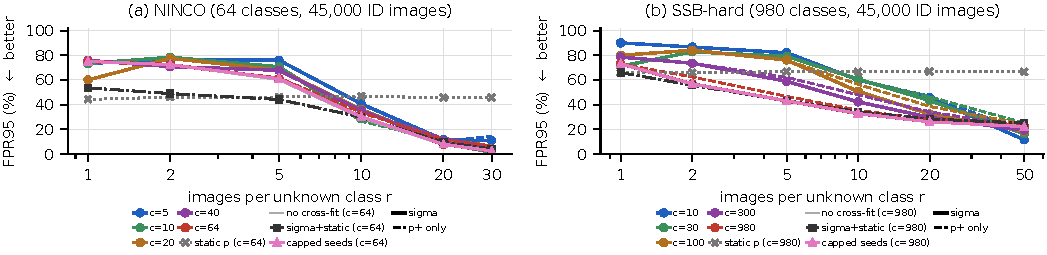
\includegraphics[width=\textwidth]{figs/fig18_rec.pdf}
\caption{再出現と混入率（\FPR{}，単体，DINOv2 L/14 + DINOv3 L/16）．IDの検証画像45,000枚に，NINCO（a）またはSSB-hard（b）から$c$個の未知クラス$\times$$r$枚を加えたテスト集合（クラスと画像の選び方を変えた3回の平均）．実線は$\sigma$，破線は$\pP$だけ，灰色の点線は静的$p$，灰色の細い実線は交差適合なしの$\pP\pN$，黒の一点鎖線は静的$p$を統計量に含めた$\sigma$，桃色は上限付きの種の$\sigma$（\secref{cap}；後四者は$c$が最大の条件）．}
\label{fig:rec}
\end{figure*}

同じクラスが何枚あり，どの混入率から効くのかを，OpenOODのIDの検証画像45,000枚に，NINCO（64クラス）またはSSB-hard（980クラス，各50枚）から$c$個の未知クラスを$r$枚ずつ加えたテスト集合で実測した（\figref{rec}，全条件は付録\ref{sec:app_rec}；未知が数枚の条件では\FPR{}の刻みが粗い）．

\textbf{再出現しない未知には静的な検出器より劣る．}$r\le5$では，$\sigma$は同じ特徴の静的$p$より\FPR{}が高い（\NRecNRLeFive{}条件中\NRecNRLeFiveMainWorseStatic{}条件，差は最大\NRecMaxMainMinusStaticLeFive{}ポイント）．NINCOの64クラス$\times$1枚では$\sigma$ \NRecNincoCSixFourROneMainFpr\%，$\pP$だけでも\NRecNincoCSixFourROneLpFpr\%に対し，静的$p$は\NRecNincoCSixFourROneStaticFpr\%である．1枚だけの未知は$k_g{=}10$本の辺をすべて外へ張るので，伝播はその画像を隣のIDに均す．$r\ge10$では逆転し（\NRecNRGeOneZero{}条件中\NRecNRGeOneZeroMainBetterStatic{}条件），NINCOの64クラス$\times$10枚で\NRecNincoCSixFourROneZeroMainFpr\%，30枚で\NRecNincoCSixFourRThreeZeroMainFpr\%（静的$p$は\NRecNincoCSixFourRThreeZeroStaticFpr\%）まで下がる．SSB-hard（兄弟クラス）は遅く，980クラス$\times$10枚で\NRecSsbCNineEightZeroROneZeroMainFpr\%，50枚で\NRecSsbCNineEightZeroRFiveZeroMainFpr\%である．

\textbf{交差適合と静的$p$．}交差適合なしの$\pP\pN$との\FPR{}の差は\NRecNAll{}条件中\NRecNMainWithinOneVOne{}条件で1ポイント以内である（灰色の細線）．$\sigma$に静的$p$を加えると，再出現しない未知での劣化は縮み（64クラス$\times$1枚で\NRecNincoCSixFourROnePpsFpr\%），$r\ge10$では\NRecNRGeOneZero{}条件中\NRecNRGeOneZeroPpsWorseMain{}条件で$\sigma$より悪い（付録\ref{sec:app_rec}）．命題4はどちらにも成り立つ．\textbf{近傍数$k_g$．}同じ格子で$k_g\in\{3,5,10,20,40\}$を変えると（付録\ref{sec:app_kg}の\figref{kg}），$k_g$が大きいほど再出現の少ない側で良く（NINCO 64クラス$\times$1枚：$k_g{=}40$で\NKgNincoKgFourZeroROneMainFpr\%，$k_g{=}10$で\NKgNincoKgOneZeroROneMainFpr\%），多い側で悪い（$\times$30枚：\NKgNincoKgFourZeroRThreeZeroMainFpr\%と\NKgNincoKgOneZeroRThreeZeroMainFpr\%）．登録時の仮説「小さい$k_g$ほど小さい$r$で静的$p$を下回る」は否定され（付録\ref{sec:app_hyp}），$k_g{=}10$は最大の$r$でNINCOの最良，SSB-hardで最良との差\NKgSsbHardKgOneZeroMinusBestRmaxFpr{}ポイントである．
\textbf{保証は条件に依らない．}$\pfin$のIDの誤警報率$\Pr(\pfin\le0.05)$は格子の全条件で\NRecFprZeroZeroFiveMin{}--\NRecFprZeroZeroFiveMax{}であり，未知の量や再出現の枚数に依らず一定である（学習画像の較正では\secref{fdp}のとおり0.05をやや超える）．


\subsection{種の数の上限：混入率が高いときの害を抑える}
\label{sec:cap}
混入率が高いと水準$q$の種はIDのほぼ全数に達し，$\pN$は情報を失う（\secref{in200}）．そこで，棄却の閾値に上限を付けた規則（\secref{seed}：$c_i=\min(q\,i/m',\,\tau)$，$\tau{=}0.05$，$q{=}0.2$）を実行前に登録し，上限なしの規則と同じ実行の中で評価した（付録\ref{sec:app_hyp}）．

\textbf{ImageNet-1Kでは変わらない．}上限が効くのはStorey型の閾値が$\tau$を超えるSSB-hardとOpenImage-O（iNaturalistではわずか）で，SSB-hardでは種が折の\NCapSeedSsbHardStoreyRatio\%から\NCapSeedSsbHardStoreycRatio\%に減り，種に混じるIDの割合は\NCapSeedSsbHardStoreyIdfrac{}から\NCapSeedSsbHardStoreycIdfrac{}に下がる．near-OODの\FPR{}は単体で\NCapStoreycAloneNearFpr\%（上限なし\NAloneNearFpr\%；対応のある差\NCapStoreycAloneNearDfprVsStorey{} [\NCapStoreycAloneNearDfprVsStoreyLo, +\NCapStoreycAloneNearDfprVsStoreyHi]），$\times$TINSで\NCapStoreycNearFpr\%（+\NCapStoreycNearDfprVsStorey{}），far-OODとFour-OODの単体は\NCapStoreycAloneFarFpr\%，\NCapStoreycAloneFourFpr\%で，いずれも上限なしと0.25ポイント以内である．

\textbf{混入率が高いベンチマークでは害がほぼ消える．}ImageNet-200のnear-OODでは\FPR{}が\NInTwoZeroZeroMainNearFpr\%から\NInTwoZeroZeroStoreycNearFpr\%へ下がり（差\NInTwoZeroZeroStoreycNearDfprVsStorey{} [\NInTwoZeroZeroStoreycNearDfprVsStoreyLo, \NInTwoZeroZeroStoreycNearDfprVsStoreyHi]），$\pP$だけ（\NInTwoZeroZeroLpNearFpr\%）より\NInTwoZeroZeroStoreycNearDfprVsLpAbs{}ポイント低い（[\NInTwoZeroZeroStoreycNearDfprVsLpLo, \NInTwoZeroZeroStoreycNearDfprVsLpHi]）．far-OODは\NInTwoZeroZeroStoreycFarFpr\%で$\pP$だけ（\NInTwoZeroZeroLpFarFpr\%）と並ぶ．CIFAR-100ではnear-OODが\NCifarMainNearFpr\%から\NCifarStoreycNearFpr\%（$\pP$だけ\NCifarLpNearFpr\%），far-OODが\NCifarMainFarFpr\%から\NCifarStoreycFarFpr\%になり，$\pP$だけ（\NCifarLpFarFpr\%）との差は+\NCifarMainFarDfprVsLp{}から+\NCifarStoreycFarDfprVsLp{} [\NCifarStoreycFarDfprVsLpLo, \NCifarStoreycFarDfprVsLpHi]ポイントに縮む．\secref{rec}の格子の\NCaprecNCells{}条件でも，上限付きの規則が$\pP$だけより1ポイント以上悪い条件は混入率30\%以上の\NCaprecNHi{}条件で\NCaprecStoreycHiNWorseLpOne{}，$r\ge10$・混入率30\%未満の\NCaprecLoROneZeroN{}条件では上限なしとの差が最大\NCaprecLoROneZeroMaxStoreycMinusStorey{}ポイントと利得を保つ（付録\ref{sec:app_cap}）．

\textbf{位置づけ．}本稿の主構成は登録どおり上限なしのStorey型であり（\tabref{main}），上限付きは登録済みの変種として報告する．上限付きの種はCIFAR-100 far-OODの+\NCifarStoreycFarDfprVsLp{}ポイントを除いて$\pP$だけと同等以上で，ImageNet-1Kでは上限なしと変わらないから，混入率が未知の運用には上限付きを推す．


\subsection{最終スコアの保証の実測}
\label{sec:fdp}
命題4は折の較正画像とIDのテスト画像の交換可能性を仮定するが，ベンチマークでは前者が学習画像，後者が検証画像である．較正画像をIDの検証画像から取った交換可能な設定（\NVcalNSplits{}通り，付録\ref{sec:app_fdp}）では，IDの誤警報率$\Pr(\pfin\le\alpha)$は$\alpha{=}0.05$で\NVcalFprZeroZeroFiveMin{}--\NVcalFprZeroZeroFiveMax{}，$0.2$で\NVcalFprZeroTwoMin{}--\NVcalFprZeroTwoMax{}，BH法（$q{=}0.2$）の偽発見割合は\NVcalBhFdpMin{}--\NVcalBhFdpMax{}と水準以下で，検知性能は変わらない（near-OODの\FPR{}は単体で\NVcalAloneNearFpr\%）．命題4の保証は実測でも成り立つ．学習画像の較正では$\Pr(\pfin\le0.05)$が\NVtrainFprZeroZeroFiveMin{}--\NVtrainFprZeroZeroFiveMax{}，偽発見割合が\NVtrainBhFdpMin{}--\NVtrainBhFdpMax{}と，ずれの分だけ水準を超える．

\subsection{ImageNet-200とCIFAR-100}
\label{sec:in200}
\textbf{ImageNet-200．}構成を固定したまま単体で評価した（\NInTwoZeroZeroNDraws{}通りの抽出の平均，較正画像$n{=}800$；付録\ref{sec:app_in200}の\tabref{in200}）．$\sigma$はnear-OODで\AUC{} \NInTwoZeroZeroMainNearAuroc\%，\FPR{} \NInTwoZeroZeroMainNearFpr\%，far-OODで\NInTwoZeroZeroMainFarAuroc\%，\NInTwoZeroZeroMainFarFpr\%であり，OpenOOD v1.5~\cite{zhang2023openood}の報告値の最良（near \NInTwoZeroZeroBestPubNearAuroc\%／\NInTwoZeroZeroBestPubNearFpr\%，far \NInTwoZeroZeroBestPubFarAuroc\%／\NInTwoZeroZeroBestPubFarFpr\%；ImageNet-200で学習したResNet-18）を大きく上回る．ラベルの数を揃えない基線として，同じ2つの特徴で全学習画像258,951枚を使うkNN（$k{=}50$）とクラス平均，CLIP ViT-B/16のゼロショットのMCMとNegLabelも実測した．kNNは\FPR{} \NInTwoZeroZeroKnnAllKFiveZeroNearFpr\%／\NInTwoZeroZeroKnnAllKFiveZeroFarFpr\%，クラス平均は\NInTwoZeroZeroNcmAllNearFpr\%／\NInTwoZeroZeroNcmAllFarFpr\%で16枚の静的$p$（\NInTwoZeroZeroStaticNearFpr\%／\NInTwoZeroZeroStaticFarFpr\%）と同程度にとどまり，MCMとNegLabelは\NInTwoZeroZeroMcmClipNearFpr\%／\NInTwoZeroZeroMcmClipFarFpr\%，\NInTwoZeroZeroNeglabelClipNearFpr\%／\NInTwoZeroZeroNeglabelClipFarFpr\%である．ラベル付き画像を約80倍使っても伝播の分（$\pP$だけで\NInTwoZeroZeroLpNearFpr\%／\NInTwoZeroZeroLpFarFpr\%）は得られない．一方，上限なしの種は効かない．LGC-maxは\NInTwoZeroZeroLgcNearFpr\%／\NInTwoZeroZeroLgcFarFpr\%で，$\pN$を加えた本稿の構成はこれらより悪い．IDが9,000枚しかなく，SSB-hardでは未知が全画像の\NInTwoZeroZeroMixSsbHard\%を占めて折の全画像が種になる（付録\ref{sec:app_in200}；単純BH法の種では\NInTwoZeroZeroBhNearFpr\%）．上限付きの種（\secref{cap}）では\NInTwoZeroZeroStoreycNearFpr\%／\NInTwoZeroZeroStoreycFarFpr\%と$\pP$だけと同等以上になる．

\textbf{CIFAR-100．}OpenOOD v1.5のCIFAR-100ベンチマーク（\secref{exp}）で，同じ凍結特徴と学習画像からの16枚（クラスあたり，重ならない6通りの抽出，較正画像$n{=}400$），同じ構成で単体の値を測った（\tabref{cifar}）．$\sigma$はnear-OODで\AUC{} \NCifarMainNearAuroc\%，\FPR{} \NCifarMainNearFpr\%，far-OODで\NCifarMainFarAuroc\%，\NCifarMainFarFpr\%で，報告値（CIFAR-100で学習したResNet-18）の最良であるOE（near \NCifarBestPubNearAuroc\%／\NCifarBestPubNearFpr\%，外れ値データで学習）とRotPred（far \NCifarBestPubFarAuroc\%／\NCifarBestPubFarFpr\%）を\AUC{}で10ポイント以上上回る．全学習画像50,000枚のkNN（$k{=}50$，\NCifarKnnAllKFiveZeroNearFpr\%／\NCifarKnnAllKFiveZeroFarFpr\%）とクラス平均（\NCifarNcmAllNearFpr\%／\NCifarNcmAllFarFpr\%）は16枚の静的$p$（\NCifarStaticNearFpr\%／\NCifarStaticFarFpr\%）から数ポイント以内にとどまり，$32\times32$の画像ではゼロショットのMCMとNegLabelは弱い（\NCifarMcmClipNearFpr\%／\NCifarMcmClipFarFpr\%，\NCifarNeglabelClipNearFpr\%／\NCifarNeglabelClipFarFpr\%）．ここでも利得は$\pP$の伝播にあり，種は効かない．$\pP$だけで\NCifarLpNearFpr\%／\NCifarLpFarFpr\%，$\sigma$との差はnear-OODで\NCifarMainNearDfprVsLp{} [\NCifarMainNearDfprVsLpLo, +\NCifarMainNearDfprVsLpHi]，far-OODで+\NCifarMainFarDfprVsLp{} [+\NCifarMainFarDfprVsLpLo, +\NCifarMainFarDfprVsLpHi]ポイントで，far-OODでは$\pN$が害になる．未知がMNIST・SVHN・Places365で全画像の\NCifarMixFarHiMin{}--\NCifarMixFarHiMax\%を占め，割合$q$の種がIDのほぼ全数になって$\pN$は情報を失う（付録\ref{sec:app_in200}）．上限付きの種では近\NCifarStoreycNearFpr\%，遠\NCifarStoreycFarFpr\%になる（\secref{cap}）．


\section{結論}
支持画像からの質量を1つのグラフで伝播させ較正画像の中での順位（共形$p$値）で読む共形ラベル伝播と，再出現する未知を自己ラベル付けした種から引き上げる魚道，交差適合で読み出し$\pfin$を共形$p$値にする枠組みSalmon Ladderを提案した．凍結した特徴抽出器とクラスあたり16枚のラベル付き画像だけで，OpenOOD v1.5 ImageNet-1Kのnear-OOD（単体で\AUC{} \NAloneNearAuroc\%，\FPR{} \NAloneNearFpr\%），far-OOD，Four-OOD，ImageNet-200，CIFAR-100のすべてで公開の最良値を更新し，near-OODの\FPR{}を\NAloneNearFprRatioVsBestOther{}分の1にした．利得の大半はグラフ上の伝播にあり，同じグラフ上のクラスラベル伝播，静的な検出器，全学習画像を使うkNNでは得られず，4つのベース検出器と6つの特徴抽出器で再現する．種はImageNet-1Kのnear-OODで\FPR{}をさらに\NAloneNearDfprVsLpAbs{}ポイント下げるが，効くのは再出現がクラスあたり10枚以上で混入率が中程度のときに限られ，種の閾値に上限$\tau{=}0.05$を付けた規則が混入率の高いときの害をほぼ消す（ImageNet-200 near-OODで\NInTwoZeroZeroStoreycNearFpr\%，$\pP$だけは\NInTwoZeroZeroLpNearFpr\%）．限界は，1枚しか現れない未知には静的な検出器より劣ること，ベース検出器との積には床のない$\sigma$が要ること（登録外の形），理論が扱うのは有効性であって検知力ではないことである．


\begin{thebibliography}{99}
\footnotesize\baselineskip12\h\setlength{\itemsep}{0pt}\setlength{\parskip}{0pt}\setlength{\parsep}{0pt}
\bibitem{radford2021clip} A. Radford et al.: Learning transferable visual models from natural language supervision. \textit{ICML}, 2021.
\bibitem{ming2022mcm} Y. Ming et al.: Delving into out-of-distribution detection with vision-language representations. \textit{NeurIPS}, 2022.
\bibitem{jiang2024neglabel} X. Jiang et al.: Negative label guided OOD detection with pretrained vision-language models. \textit{ICLR}, 2024.
\bibitem{zhang2024adaneg} Y. Zhang and L. Zhang: AdaNeg: Adaptive negative proxy guided OOD detection with vision-language models. \textit{NeurIPS}, 2024.
\bibitem{zhang2026tanl} Y. Zhang et al.: Activation matters: Test-time activated negative labels for OOD detection with vision-language models. \textit{CVPR}, 2026.
\bibitem{xu2026interneg} Z. Xu et al.: Mind the way you select negative texts: Pursuing the distance consistency in OOD detection with VLMs. \textit{CVPR}, 2026.
\bibitem{yang2026tins} Y. Yang et al.: TINS: Test-time ID-prototype-separated negative semantics learning for OOD detection. arXiv:2605.10756, 2026.
\bibitem{zhang2023openood} J. Zhang et al.: OpenOOD v1.5: Enhanced benchmark for out-of-distribution detection. \textit{DMLR}, 2024.
\bibitem{park2023nnguide} J. Park, Y. G. Jung, and A. B. J. Teoh: Nearest neighbor guidance for out-of-distribution detection. \textit{ICCV}, 2023.
\bibitem{li2024moodv2} J. Li et al.: MOODv2: Masked image modeling for out-of-distribution detection. \textit{IEEE TPAMI}, 2024.
\bibitem{caetano2025discopatch} F. Caetano et al.: DisCoPatch: Taming adversarially-driven batch statistics for improved out-of-distribution detection. \textit{ICCV}, 2025.
\bibitem{marandon2024adadetect} A. Marandon, L. Lei, D. Mary, and E. Roquain: Adaptive novelty detection with false discovery rate guarantee. \textit{Ann. Stat.}, 52(1), 2024.
\bibitem{huang2021mos} R. Huang and Y. Li: MOS: Towards scaling out-of-distribution detection for large semantic space. \textit{CVPR}, 2021.
\bibitem{bates2023conformal} S. Bates, E. Cand\`{e}s, L. Lei, Y. Romano, and M. Sesia: Testing for outliers with conformal p-values. \textit{Ann. Stat.}, 51(1):149--178, 2023.
\bibitem{zhou2004lgc} D. Zhou et al.: Learning with local and global consistency. \textit{NIPS}, 2004.
\bibitem{benjamini1995bh} Y. Benjamini and Y. Hochberg: Controlling the false discovery rate: A practical and powerful approach to multiple testing. \textit{J. R. Stat. Soc. B}, 1995.
\bibitem{storey2002} J. D. Storey: A direct approach to false discovery rates. \textit{J. R. Stat. Soc. B}, 2002.
\bibitem{blanchard2008two} G. Blanchard and E. Roquain: Two simple sufficient conditions for FDR control. \textit{Electron. J. Stat.}, 2:963--992, 2008.
\bibitem{chernozhukov2018dml} V. Chernozhukov et al.: Double/debiased machine learning for treatment and structural parameters. \textit{Econom. J.}, 21(1):C1--C68, 2018.
\bibitem{oquab2024dinov2} M. Oquab et al.: DINOv2: Learning robust visual features without supervision. \textit{TMLR}, 2024.
\bibitem{simeoni2025dinov3} O. Sim\'{e}oni et al.: DINOv3. arXiv:2508.10104, 2025.
\bibitem{scott2009novelty} C. Scott and G. Blanchard: Novelty detection: Unlabeled data definitely help. \textit{AISTATS}, pp.~464--471, 2009.
\bibitem{blanchard2010ssnd} G. Blanchard, G. Lee, and C. Scott: Semi-supervised novelty detection. \textit{J. Mach. Learn. Res.}, 11:2973--3009, 2010.
\bibitem{haroush2022statistical} M. Haroush, T. Frostig, R. Heller, and D. Soudry: A statistical framework for efficient out of distribution detection in deep neural networks. \textit{ICLR}, 2022.
\bibitem{liang2024integrative} Z. Liang, M. Sesia, and W. Sun: Integrative conformal p-values for out-of-distribution testing with labelled outliers. \textit{J. R. Stat. Soc. B}, 86(3):671--693, 2024.
\bibitem{liu2019tpn} Y. Liu et al.: Learning to propagate labels: Transductive propagation network for few-shot learning. \textit{ICLR}, 2019.
\bibitem{yang2025oodd} Y. Yang et al.: OODD: Test-time out-of-distribution detection with dynamic dictionary. \textit{CVPR}, 2025.
\bibitem{fan2024rtl} K. Fan et al.: Test-time linear out-of-distribution detection. \textit{CVPR}, pp.~23752--23761, 2024.
\bibitem{yang2023auto} P. Yang, J. Liang, J. Cao, and R. He: AUTO: Adaptive outlier optimization for test-time OOD detection. arXiv:2303.12267, 2023.
\bibitem{sun2022knn} Y. Sun, Y. Ming, X. Zhu, and Y. Li: Out-of-distribution detection with deep nearest neighbors. \textit{ICML}, 2022.
\bibitem{caron2021dino} M. Caron et al.: Emerging properties in self-supervised vision transformers. \textit{ICCV}, 2021.
\bibitem{xu2024scale} K. Xu et al.: Scaling for training time and post-hoc out-of-distribution detection enhancement. \textit{ICLR}, 2024.
\bibitem{song2022rankfeat} Y. Song, N. Sebe, and W. Wang: RankFeat: Rank-1 feature removal for out-of-distribution detection. \textit{NeurIPS}, 2022.
\bibitem{chen2024csp} M. Chen, J. Gao, and C. Xu: Conjugated semantic pool improves OOD detection with pre-trained vision-language models. \textit{NeurIPS}, 2024.
\end{thebibliography}


\clearpage
\appendix
\section{命題1と命題2の証明}
\label{sec:app_proofs}
\textbf{命題1．}$S\bom=D^{-1/2}WD^{-1/2}D^{1/2}\mathbf{1}=D^{-1/2}W\mathbf{1}=\bom$であり，$S$は対称なので$\bom^{\top}S=\bom^{\top}$．よって$\bom^{\top}\mathbf{u}^{(\ell+1)}=\lambda\bom^{\top}\mathbf{u}^{(\ell)}+(1-\lambda)\bom^{\top}\mathbf{y}^{+}$となり，$\mathbf{u}^{(0)}=\mathbf{0}$から解けば$\bom^{\top}\mathbf{u}^{(L)}=(1-\lambda^{L})\bom^{\top}\mathbf{y}^{+}=(1-\lambda^{L})\sum_{j\in\mathcal{S}}\sqrt{\delta_j}$を得る．$\square$

\textbf{命題4．}$\sigma$を折$b$の節点の上の関数とみる．それを定めるのは，支持画像，折$\bar b$の節点とその較正・テストの区別，および「$\mathcal{C}_b\cup\mathcal{T}_b$という節点の集合」だけである．グラフと$\mathbf{u}^{+}$は節点の名札に依らず（\secref{graph}），$\hat{Q}_{\bar b}$と$\mathbf{u}^{-}_{\bar b}$は折$\bar b$の画像と$\mathbf{u}^{+}$から決まり，参照する較正画像は$\mathcal{C}_{\bar b}$である．したがって$\sigma$は，$\mathcal{C}_b\cup\mathcal{T}_b$の中でどの節点を較正画像と呼ぶかを入れ替えても変わらない．これはAdaDetectの条件(8)（学習標本を支持画像と折$\bar b$の全節点，帰無の較正標本を$\mathcal{C}_b$，テスト標本を$\mathcal{T}_b$としたもの．同論文の証明は学習標本を所与とした置換の議論なので，その中身は問わない）であり，\eqnref{pfin}の$\pfin$は同論文の経験$p$値(10)である．よって定理3.3から(i)と(ii)のPRDS・超一様性が従い，系3.5と系3.7がFDRの上界を与える．$\square$

\textbf{系1．}\eqnref{walk}のランダムウォーク（各ステップで確率$1-\lambda$で止まる）で，$Q$から初めて外へ出る時刻を$\tau$とする．$Q\cap Y=\emptyset$なので$X_T\in Y$には$\tau\le T$が要り，止まる時刻$T$は幾何分布で無記憶だから，強マルコフ性より$u_i/\sqrt{\delta_i}=\mathbb{E}_i[\mathbf{1}[\tau\le T]\,u_{X_\tau}/\sqrt{\delta_{X_\tau}}]\le\Pr_i(\tau\le T)\max_{j\in\partial Q}u_j/\sqrt{\delta_j}$（$X_\tau\in\partial Q$）．$\pi_i=\Pr_i(\tau\le T)$は最初の1歩で分けると$\pi_i=\lambda(e_i+\sum_{j\in Q}P_{ij}\pi_j)$，すなわち$\boldsymbol{\pi}=\lambda(I-\lambda P_{QQ})^{-1}\mathbf{e}$を満たす（$\lambda P_{QQ}$のスペクトル半径は1未満）．$\pi^{*}=\max_{x\in Q}\pi_x$は$e_x\le\bar e_Q$から$\pi^{*}\le\lambda(\bar e_Q+(1-\bar e_Q)\pi^{*})$，すなわち$\pi^{*}\le\psi(\bar e_Q)$を満たす．$u^{+}_{x'}\le u^{+}_i$なら$u^{+}_{x'}\le b_i$なので，\eqnref{plp}の数え上げから第2式が従い，$\bar e_Q=0$なら$\boldsymbol{\pi}=\mathbf{0}$，$u^{+}_i=0$である．$\square$

\textbf{命題2．}$i\in Q$では$y_i=0$なので$u_i=\lambda\sum_jW_{ij}u_j/\sqrt{\delta_i\delta_j}$．両辺に$\sqrt{\delta_i}$を掛けて$Q$で足すと，$Q$の内側の辺からの寄与は$\sum_{j\in Q}(u_j/\sqrt{\delta_j})\sum_{i\in Q}W_{ij}\le\sum_{j\in Q}\sqrt{\delta_j}u_j$で抑えられ，外側の辺からの寄与は$w(Q,\bar{Q})\max_{j}u_j/\sqrt{\delta_j}$で抑えられる．\eqnref{walk}と同じランダムウォークの表現より$u_j/\sqrt{\delta_j}\le1/\min_{s\in Y}\sqrt{\delta_s}$なので，移項して\eqnref{cond}を得る．$\square$

\section{最終読み出しの保証の実測と種に混じるIDの割合}
\label{sec:app_fdp}
\secref{fdp}の2つの設定の詳細を示す．

\textbf{交換可能な較正（検証画像）．}較正画像をIDの検証画像からクラスあたり4枚取り（残りの検証画像がIDのテスト集合），支持画像は学習画像のままにすると，較正画像とIDのテスト画像は交換可能になる．\NVcalNSplits{}通りの抽出・9データセットで，IDの誤警報率$\Pr(\pfin\le\alpha)$は$\alpha{=}0.01$で\NVcalFprZeroZeroOneMin{}--\NVcalFprZeroZeroOneMax{}，$0.05$で\NVcalFprZeroZeroFiveMin{}--\NVcalFprZeroZeroFiveMax{}，$0.1$で\NVcalFprZeroOneMin{}--\NVcalFprZeroOneMax{}，$0.2$で\NVcalFprZeroTwoMin{}--\NVcalFprZeroTwoMax{}とどの水準でも$\alpha$のまわりに収まり，$\pfin$へのBH法（$q{=}0.2$）の偽発見割合は\NVcalBhFdpMin{}--\NVcalBhFdpMax{}で水準以下，その再現率（未知のうち棄却された割合）は\NVcalBhRecallMin{}--\NVcalBhRecallMax{}である．種に混じるIDの割合（折ごと，命題3の対象）も$q{=}0.2$で\NVcalIdfracStoreyMin{}--\NVcalIdfracStoreyMax{}（Storey型）である．検知性能は学習画像の較正と変わらない（near-OODの\FPR{}は$\times$TINSで\NVcalMainNearFpr\%，単体で\NVcalAloneNearFpr\%）．命題4の保証は実測でも成り立つ．

\textbf{ベンチマークの較正（学習画像）．}同じ量を\tabref{main}の設定（6通りの抽出）で測ると，$\Pr(\pfin\le0.05)$は\NVtrainFprZeroZeroFiveMin{}--\NVtrainFprZeroZeroFiveMax{}，BH法の偽発見割合は\NVtrainBhFdpMin{}--\NVtrainBhFdpMax{}，種のIDの割合は\NVtrainIdfracStoreyMin{}--\NVtrainIdfracStoreyMax{}（単純BH法では\NVtrainIdfracBhMin{}--\NVtrainIdfracBhMax{}）であり，学習画像と検証画像のずれの分だけ水準を超える（\tabref{fdp}）．ベンチマークの値（\tabref{main}）はその定めどおり学習画像の較正で報告する．


\tabref{val}に，交換可能な較正での$\pfin$の実測の誤警報率とBH法の偽発見割合をデータセット別に示す．\tabref{fdp}に，\tabref{main}の設定（学習画像の較正，$q{=}0.2$，6通りの抽出の平均）で折ごとに選ばれた種の数（2つの折の平均）と，種に混じっていたIDの割合（実測の偽発見割合）を，Storey型と単純BH法の両方について，データセット別・ビュー別に示す（\secref{fdp}）．交換可能な較正での同じ量は\secref{fdp}の本文に範囲で示した．

\begin{table}[t]
\centering
\caption{最終スコア$\pfin$の保証の実測（交換可能な較正：IDの検証画像からクラスあたり4枚を較正画像とし，\NVcalNSplits{}通りの抽出の平均，単体）．IDの誤警報率は$\pfin\le\alpha$と判定されたIDのテスト画像の割合（命題4(i)：$\le\alpha$），偽発見割合はBH法（$q{=}0.2$）で棄却された画像のうちIDの割合（命題4(ii)：期待値$\le0.2$），再現率は未知のうち棄却された割合．}
\label{tab:val}
\vspace{1.5mm}
{\fontsize{6.5pt}{7.6pt}\selectfont\renewcommand{\arraystretch}{1.0}%
\setlength{\tabcolsep}{1.7pt}\begin{tabular}{@{}lcccc|cc@{}}
\hline
\rule[-2.0pt]{0pt}{8.6pt} & \multicolumn{4}{c|}{IDの誤警報率 $\Pr(\pfin\le\alpha)$} & \multicolumn{2}{c}{BH法（$q{=}0.2$）} \\
\rule[-2.0pt]{0pt}{8.6pt}データセット & $\alpha{=}0.01$ & $0.05$ & $0.1$ & $0.2$ & 偽発見割合 & 再現率 \\
\hline
SSB-hard & 0.009 & 0.051 & 0.099 & 0.201 & 0.091 & 0.901 \\
NINCO & 0.011 & 0.052 & 0.100 & 0.197 & 0.183 & 0.983 \\
iNaturalist & 0.009 & 0.049 & 0.099 & 0.198 & 0.158 & 0.998 \\
Textures & 0.011 & 0.054 & 0.103 & 0.202 & 0.191 & 0.928 \\
OpenImage-O & 0.009 & 0.051 & 0.103 & 0.199 & 0.147 & 0.901 \\
iNat. (Four-OOD) & 0.009 & 0.050 & 0.101 & 0.203 & 0.165 & 0.998 \\
SUN & 0.010 & 0.051 & 0.097 & 0.200 & 0.168 & 0.981 \\
Places & 0.009 & 0.050 & 0.099 & 0.198 & 0.165 & 0.855 \\
Textures (Four-OOD) & 0.011 & 0.051 & 0.102 & 0.203 & 0.191 & 0.915 \\
\hline
\end{tabular}}%

\end{table}

\begin{table}[t]
\centering
\caption{学習画像の較正で選ばれた種（折あたり，6通りの抽出の平均）．種は種の数，ID率は種に混じっていたIDの割合（実測の偽発見割合，水準$q{=}0.2$）．}
\label{tab:fdp}
\vspace{1.5mm}
{\fontsize{6.0pt}{7.1pt}\selectfont\renewcommand{\arraystretch}{1.0}%
\setlength{\tabcolsep}{1.3pt}\begin{tabular}{@{}lcccc|cccc@{}}
\hline
\rule[-2.0pt]{0pt}{8.2pt} & \multicolumn{4}{c|}{DINOv2 L/14} & \multicolumn{4}{c}{DINOv3 L/16} \\
\rule[-2.0pt]{0pt}{8.2pt} & \multicolumn{2}{c}{Storey型} & \multicolumn{2}{c|}{単純BH} & \multicolumn{2}{c}{Storey型} & \multicolumn{2}{c}{単純BH} \\
\rule[-2.0pt]{0pt}{8.2pt}データセット & 種 & ID率 & 種 & ID率 & 種 & ID率 & 種 & ID率 \\
\hline
SSB-hard & 30,383 & 0.219 & 23,993 & 0.102 & 31,030 & 0.230 & 24,227 & 0.103 \\
NINCO & 3,784 & 0.254 & 3,597 & 0.219 & 3,993 & 0.281 & 3,685 & 0.226 \\
iNaturalist & 6,642 & 0.249 & 6,197 & 0.196 & 6,808 & 0.266 & 6,240 & 0.200 \\
Textures & 3,064 & 0.248 & 2,892 & 0.213 & 3,277 & 0.278 & 3,030 & 0.230 \\
OpenImage-O & 9,433 & 0.235 & 8,281 & 0.167 & 9,932 & 0.256 & 8,584 & 0.174 \\
iNat. (Four-OOD) & 6,653 & 0.250 & 6,235 & 0.201 & 6,895 & 0.276 & 6,326 & 0.211 \\
SUN & 6,414 & 0.249 & 5,911 & 0.192 & 6,668 & 0.266 & 6,075 & 0.199 \\
Places & 5,587 & 0.246 & 5,071 & 0.196 & 5,960 & 0.260 & 5,313 & 0.196 \\
Textures (Four-OOD) & 3,325 & 0.255 & 3,103 & 0.214 & 3,492 & 0.272 & 3,253 & 0.230 \\
\hline
\end{tabular}}%

\end{table}

\section{データセット別の値と散布図}
\label{sec:app_four}
\tabref{perds}と\tabref{four}に\tabref{main}のデータセット別の値を示す（\secref{main}）．\figref{scatter}は\tabref{main}の全手法の\AUC{}と\FPR{}の散布図である．

\begin{table*}[t]
\centering
\caption{OpenOOD v1.5 ImageNet-1Kのデータセット別の結果（[\%]，AUROC$\uparrow$／FPR95$\downarrow$）．記法は\tabref{main}と同じ．TINSの報告値は原論文の表8のとおりで，iNaturalistとTexturesは同論文のFour-OODの表1と同じ値が報告されている（\tabref{four}）．}
\label{tab:perds}
\vspace{1.5mm}
{\fontsize{7pt}{8.2pt}\selectfont\renewcommand{\arraystretch}{1.0}%
\setlength{\tabcolsep}{2.0pt}\begin{tabular}{@{}lcccccccccc@{}}
\hline
\rule[-2.0pt]{0pt}{8.6pt} & \multicolumn{4}{c}{near-OOD} & \multicolumn{6}{c}{far-OOD} \\
\rule[-2.0pt]{0pt}{8.6pt} & \multicolumn{2}{c}{SSB-hard} & \multicolumn{2}{c}{NINCO} & \multicolumn{2}{c}{iNaturalist} & \multicolumn{2}{c}{Textures} & \multicolumn{2}{c}{OpenImage-O} \\
\rule[-2.0pt]{0pt}{8.6pt}手法 & AUROC & FPR95 & AUROC & FPR95 & AUROC & FPR95 & AUROC & FPR95 & AUROC & FPR95 \\
\hline
MOODv2~\cite{li2024moodv2}$^{\dagger}$ & 85.00 & 58.10 & 92.70 & 38.20 & 99.60 & 1.80 & 94.30 & 24.70 & 97.40 & 13.60 \\
NNGuide~\cite{park2023nnguide}$^{\dagger}$ & 84.70 & 54.70 & 93.70 & 28.90 & 99.90 & 1.80 & 95.80 & 17.00 & 97.70 & 10.80 \\
RankFeat~\cite{song2022rankfeat}$^{\dagger}$ & 89.40 & 47.90 & 90.00 & 39.30 & 96.00 & 13.00 & 95.00 & 25.40 & 92.40 & 33.30 \\
SCALE~\cite{xu2024scale}$^{\dagger}$ & 77.40 & 67.70 & 85.40 & 51.80 & 98.00 & 9.50 & 97.60 & 11.90 & 94.00 & 28.20 \\
DisCoPatch~\cite{caetano2025discopatch}$^{\dagger}$ & 95.80 & 19.80\sota & 94.30 & 39.00 & 99.10 & 3.60 & 96.40 & 18.90 & 94.40 & 29.70 \\
TINS~\cite{yang2026tins}$^{\dagger}$ & 81.38 & 61.68 & 83.91 & 54.09 & 99.93 & 0.21 & 97.83 & 10.09 & 92.99 & 28.68 \\
TINS~\cite{yang2026tins}（実測） & 82.22 & 56.65 & 80.74 & 56.09 & 99.93 & 0.17 & 98.11 & 8.31 & 93.09 & 28.20 \\
Salmon Ladder，単体 & \cellcolor{upd}\textbf{96.24} & 21.72 & \cellcolor{upd}\textbf{99.65} & \cellcolor{upd}\textbf{1.28} & 99.93 & \cellcolor{upd}\textbf{0.16} & \cellcolor{upd}\textbf{98.91} & \cellcolor{upd}\textbf{4.37} & 97.55 & 10.98 \\
Salmon Ladder $\times$TINS & \cellcolor{upd}\textbf{96.51}\sota & 19.96 & \cellcolor{upd}\textbf{99.68}\sota & \cellcolor{upd}\textbf{1.03}\sota & \cellcolor{upd}\textbf{99.96}\sota & \cellcolor{upd}\textbf{0.11}\sota & \cellcolor{upd}\textbf{99.31}\sota & \cellcolor{upd}\textbf{2.56}\sota & \cellcolor{upd}\textbf{97.87}\sota & \cellcolor{upd}\textbf{9.81}\sota \\
{\scriptsize\textcolor{black!60}{\quad 最良の比較手法との差}} & \gap{+0.71} & \gap{-0.16} & \gap{+5.38} & \gap{+27.87} & \gap{+0.03} & \gap{+0.06} & \gap{+1.20} & \gap{+5.75} & \gap{+0.17} & \gap{+0.99} \\
\hline
\end{tabular}}%

\end{table*}

\begin{figure*}[t]
\centering
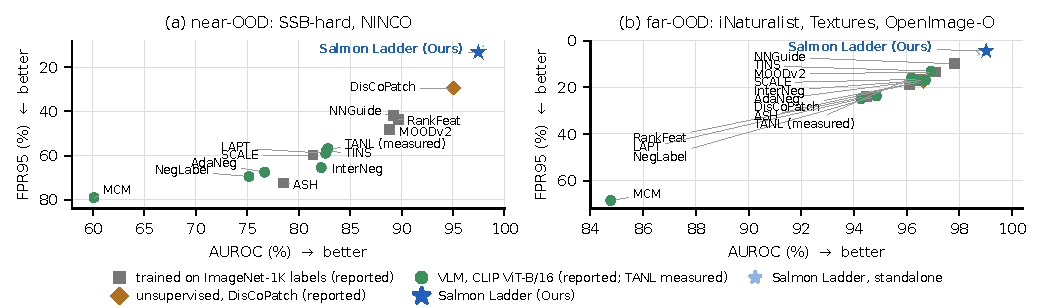
\includegraphics[width=\textwidth]{figs/fig18_scatter.pdf}
\caption{OpenOOD v1.5 ImageNet-1Kでの\AUC{}と\FPR{}（\tabref{main}の全手法，右上ほど良い）．大きな星が本稿の構成（$\times$TINS），小さな星は単体．比較手法は報告値（TANLのみ実測）．}
\label{fig:scatter}
\end{figure*}

\begin{table*}[t]
\centering
\caption{Four-OOD（ImageNet-1Kに対するiNaturalist，SUN，Places，Textures，[\%]）．比較手法はすべてCLIP ViT-B/16による報告値$\dagger$（TINSは実測も併記）．記法は\tabref{main}と同じ．}
\label{tab:four}
\vspace{1.5mm}
{\fontsize{7pt}{8.2pt}\selectfont\renewcommand{\arraystretch}{1.0}%
\setlength{\tabcolsep}{2.0pt}\begin{tabular}{@{}lcccccccccc@{}}
\hline
\rule[-2.0pt]{0pt}{8.6pt} & \multicolumn{2}{c}{iNaturalist} & \multicolumn{2}{c}{SUN} & \multicolumn{2}{c}{Places} & \multicolumn{2}{c}{Textures} & \multicolumn{2}{c}{平均} \\
\rule[-2.0pt]{0pt}{8.6pt}手法 & AUROC & FPR95 & AUROC & FPR95 & AUROC & FPR95 & AUROC & FPR95 & AUROC & FPR95 \\
\hline
MCM~\cite{ming2022mcm}$^{\dagger}$ & 94.59 & 32.20 & 92.25 & 38.80 & 90.31 & 46.20 & 86.12 & 58.50 & 90.82 & 43.93 \\
NegLabel~\cite{jiang2024neglabel}$^{\dagger}$ & 99.49 & 1.91 & 95.49 & 20.53 & 91.64 & 35.59 & 90.22 & 43.56 & 94.21 & 25.40 \\
CSP~\cite{chen2024csp}$^{\dagger}$ & 99.60 & 1.54 & 96.66 & 13.66 & 92.90 & 29.32 & 93.86 & 25.52 & 95.76 & 17.51 \\
OODD~\cite{yang2025oodd}$^{\dagger}$ & 99.79 & 0.85 & 97.17 & 12.94 & 92.51 & 30.68 & 94.51 & 30.67 & 96.00 & 18.79 \\
AdaNeg~\cite{zhang2024adaneg}$^{\dagger}$ & 99.71 & 0.59 & 97.44 & 9.50 & 94.55 & 34.34 & 94.93 & 31.27 & 96.66 & 18.92 \\
InterNeg~\cite{xu2026interneg}$^{\dagger}$ & 99.79 & 0.40 & 98.68 & 6.78 & 95.01 & 27.11 & 96.26 & 21.85 & 97.43 & 14.04 \\
TINS~\cite{yang2026tins}$^{\dagger}$ & 99.93 & 0.21 & 99.14 & 3.84 & 97.14 & 12.73 & 97.83 & 10.09 & 98.51 & 6.72 \\
TINS~\cite{yang2026tins}（実測） & 99.93 & 0.22 & 99.12 & 4.35 & 97.12 & 12.98 & 97.94 & 9.83 & 98.52 & 6.85 \\
Salmon Ladder，単体 & 99.92 & \cellcolor{upd}\textbf{0.16} & \cellcolor{upd}\textbf{99.49} & \cellcolor{upd}\textbf{1.63} & 97.05 & \cellcolor{upd}\textbf{11.35} & \cellcolor{upd}\textbf{98.72} & \cellcolor{upd}\textbf{5.12} & \cellcolor{upd}\textbf{98.80} & \cellcolor{upd}\textbf{4.56} \\
Salmon Ladder $\times$TINS & \cellcolor{upd}\textbf{99.96}\sota & \cellcolor{upd}\textbf{0.11}\sota & \cellcolor{upd}\textbf{99.66}\sota & \cellcolor{upd}\textbf{0.97}\sota & \cellcolor{upd}\textbf{97.55}\sota & \cellcolor{upd}\textbf{9.26}\sota & \cellcolor{upd}\textbf{99.18}\sota & \cellcolor{upd}\textbf{3.20}\sota & \cellcolor{upd}\textbf{99.09}\sota & \cellcolor{upd}\textbf{3.39}\sota \\
{\scriptsize\textcolor{black!60}{\quad 最良の比較手法との差}} & \gap{+0.03} & \gap{+0.10} & \gap{+0.52} & \gap{+2.87} & \gap{+0.41} & \gap{+3.47} & \gap{+1.24} & \gap{+6.63} & \gap{+0.57} & \gap{+3.33} \\
\hline
\end{tabular}}%

\end{table*}

\section{ImageNet-200とCIFAR-100}
\label{sec:app_in200}
\tabref{in200}と\tabref{cifar}に\secref{in200}のImageNet-200とCIFAR-100の値を示す．CIFAR-100のIDの誤警報率$\Pr(\pfin\le0.05)$は\NCifarValNearFprZeroZeroFive{}（near）／\NCifarValFarFprZeroZeroFive{}（far），BH法の偽発見割合は\NCifarValNearBhfdp{}／\NCifarValFarBhfdp{}である（学習画像の較正）．CIFAR-100の$32\times32$の画像は他と同じ前処理で拡大して入力し，TexturesはImageNet-1Kベンチマークと同じ画像ファイルなので特徴を共有する．CIFAR-100の種は，Storey型$q{=}0.2$でCIFAR-10・Tiny ImageNetでは折の\NCifarSeedNearStoreyRatioMin{}--\NCifarSeedNearStoreyRatioMax\%，MNIST・SVHN・Places365では\NCifarSeedFarHiStoreyRatioMin{}--\NCifarSeedFarHiStoreyRatioMax\%，Texturesでは\NCifarSeedTextureStoreyRatio\%を占め，種に混じるIDの割合は\NCifarSeedStoreyIdfracMin{}--\NCifarSeedStoreyIdfracMax{}である（DINOv3 L/16のビュー，2つの折・6通りの抽出の平均）．単純BH法の種は折の\NCifarSeedTextureBhRatio{}--\NCifarSeedMnistBhRatio\%，IDの割合\NCifarSeedMnistBhIdfrac{}--\NCifarSeedTinBhIdfrac{}である．種に混じるIDの割合は命題3どおり$q$以下でも，割合$q$の種がIDのほぼ全数になって$\pN$は情報を失う（Places365：$\sigma$ \NCifarMainPlacesThreeSixFiveFpr\%，$\pP$だけ\NCifarLpPlacesThreeSixFiveFpr\%，単純BH法の種で\NCifarBhPlacesThreeSixFiveFpr\%，上限付きの種で\NCifarStoreycPlacesThreeSixFiveFpr\%）．ImageNet-200のSSB-hardでは未知が全画像の\NInTwoZeroZeroMixSsbHard\%を占めてStorey型の$\hat{\pi}_0$が\NInTwoZeroZeroSeedSsbHardStoreyPiZero{}になり，水準$q/\hat{\pi}_0$が1を超えて折の全画像が種になる（単純BH法の種は折の\NInTwoZeroZeroSeedSsbHardBhRatioPct\%，上限付きの種は\NInTwoZeroZeroSeedSsbHardStoreycRatioPct\%，IDの割合\NInTwoZeroZeroSeedSsbHardStoreycIdfrac{}）．

\begin{table}[t]
\centering
\caption{OpenOOD v1.5 CIFAR-100（[\%]，単体，\NCifarNDraws{}通りの抽出の平均）．$\dagger$はOpenOOD v1.5~\cite{zhang2023openood}の報告値（\AUC{}は論文の表2，\FPR{}は同論文の脚注6が指す公開の表）．全学習画像のkNN・クラス平均は本稿と同じ2つの特徴（L2正規化して連結），ゼロショットはCLIP ViT-B/16（\secref{in200}）．上限付きの種は$\tau{=}0.05$（\secref{cap}）．\textcolor{sotacol}{$\bigstar$}は列の最良値，\colorbox{upd}{青}は本手法以外の全行（報告値，全学習画像・ゼロショットの基線，静的検出器，LGC-max）を上回る値．}
\label{tab:cifar}
\vspace{1.5mm}
{\fontsize{6.8pt}{8pt}\selectfont\renewcommand{\arraystretch}{1.0}%
\setlength{\tabcolsep}{2pt}\begin{tabular}{@{}lcccc@{}}
\hline
\rule[-2.0pt]{0pt}{8.6pt} & \multicolumn{2}{c}{near-OOD} & \multicolumn{2}{c}{far-OOD} \\
\rule[-2.0pt]{0pt}{8.6pt}手法 & AUROC$\uparrow$ & FPR95$\downarrow$ & AUROC$\uparrow$ & FPR95$\downarrow$ \\
\hline
\multicolumn{5}{@{}l}{\rule{0pt}{6.6pt}\textit{CIFAR-100で学習したResNet-18（報告値$^{\dagger}$）}} \\
MSP$^{\dagger}$ & 80.27 & 54.80 & 77.76 & 58.70 \\
MLS$^{\dagger}$ & 81.05 & 55.47 & 79.67 & 56.73 \\
RMDS$^{\dagger}$ & 80.15 & 55.46 & 82.92 & 52.81 \\
VOS$^{\dagger}$ & 80.93 & 55.56 & 81.32 & 53.70 \\
G-ODIN$^{\dagger}$ & 77.15 & 67.58 & 85.67 & 42.68 \\
RotPred$^{\dagger}$ & 76.43 & 62.58 & 88.40 & 34.50 \\
OE$^{\dagger}$（外れ値データで学習） & 88.30 & 30.73 & 81.41 & 54.82 \\
\multicolumn{5}{@{}l}{\rule{0pt}{6.6pt}\textit{全学習画像（50,000枚）またはゼロショット（本稿で実測）}} \\
kNN，全学習画像（$k{=}50$） & 97.09 & 16.35 & 94.94 & 32.15 \\
クラス平均，全学習画像 & 97.61 & 12.91 & 95.38 & 28.05 \\
MCM~\cite{ming2022mcm}，ゼロショット & 70.30 & 94.06 & 74.59 & 89.10 \\
NegLabel~\cite{jiang2024neglabel}，ゼロショット & 72.98 & 76.98 & 80.25 & 64.84 \\
\multicolumn{5}{@{}l}{\rule{0pt}{6.6pt}\textit{凍結特徴，クラスあたり16枚，学習なし，単体（6通りの抽出の平均）}} \\
静的$p$（グラフなし） & 96.94 & 16.49 & 94.88 & 29.19 \\
kNN（グラフなし） & 92.35 & 39.22 & 88.47 & 49.80 \\
LGC-max & 98.80 & 5.39 & 99.42 & 2.21 \\
$\pP$のみ & \cellcolor{upd}\textbf{99.11} & \cellcolor{upd}\textbf{2.88} & \cellcolor{upd}\textbf{99.57} & \cellcolor{upd}\textbf{1.22} \\
$\pP\pN$，交差適合なし & \cellcolor{upd}\textbf{99.25} & \cellcolor{upd}\textbf{2.83} & 99.35 & 2.58 \\
$\sigma$（本稿の構成） & \cellcolor{upd}\textbf{99.18} & \cellcolor{upd}\textbf{2.90} & 99.37 & 2.34 \\
$\sigma$に静的$p$を加える & \cellcolor{upd}\textbf{99.34}\sota & \cellcolor{upd}\textbf{2.60} & \cellcolor{upd}\textbf{99.64}\sota & \cellcolor{upd}\textbf{1.00}\sota \\
$\sigma$，DINOv3 L/16のみ & \cellcolor{upd}\textbf{98.95} & \cellcolor{upd}\textbf{3.77} & 99.15 & 3.48 \\
$\sigma$，上限付きの種（Storey型） & \cellcolor{upd}\textbf{99.26} & \cellcolor{upd}\textbf{2.55}\sota & \cellcolor{upd}\textbf{99.59} & \cellcolor{upd}\textbf{1.46} \\
$\sigma$，上限付きの種（単純BH法） & \cellcolor{upd}\textbf{99.26} & \cellcolor{upd}\textbf{2.55}\sota & \cellcolor{upd}\textbf{99.59} & \cellcolor{upd}\textbf{1.46} \\
\hline
\end{tabular}}%

\end{table}


\begin{table}[t]
\centering
\caption{OpenOOD v1.5 ImageNet-200（[\%]，単体，\NInTwoZeroZeroNDraws{}通りの抽出の平均）．$\dagger$はOpenOOD v1.5~\cite{zhang2023openood}の報告値（ImageNet-200で学習したResNet-18；リーダーボードと同論文の脚注6が指す公開の表）．全学習画像のkNN・クラス平均は本稿と同じ2つの特徴，ゼロショットはCLIP ViT-B/16（\secref{in200}）．上限付きの種は$\tau{=}0.05$（\secref{cap}）．\textcolor{sotacol}{$\bigstar$}は列の最良値，\colorbox{upd}{青}は本手法以外の全行（報告値，全学習画像・ゼロショットの基線，静的検出器，LGC-max）を上回る値．}
\label{tab:in200}
\vspace{1.5mm}
{\fontsize{6.8pt}{8pt}\selectfont\renewcommand{\arraystretch}{1.0}%
\setlength{\tabcolsep}{2pt}\begin{tabular}{@{}lcccc@{}}
\hline
\rule[-2.0pt]{0pt}{8.6pt} & \multicolumn{2}{c}{near-OOD} & \multicolumn{2}{c}{far-OOD} \\
\rule[-2.0pt]{0pt}{8.6pt}手法 & AUROC$\uparrow$ & FPR95$\downarrow$ & AUROC$\uparrow$ & FPR95$\downarrow$ \\
\hline
\multicolumn{5}{@{}l}{\rule{0pt}{6.6pt}\textit{ImageNet-200で学習したResNet-18（報告値$^{\dagger}$）}} \\
OE$^{\dagger}$（外れ値データで学習） & 84.84 & 52.30 & 89.02 & 34.17 \\
RegMixup + MSP$^{\dagger}$ & 84.13 & 53.78 & 90.81 & 33.88 \\
TempScale$^{\dagger}$（事後手法の最良） & 83.69 & 54.82 & 90.82 & 34.00 \\
PixMix + ASH$^{\dagger}$ & 81.36 & 63.51 & 95.01 & 21.22 \\
NPOS$^{\dagger}$ & 79.40 & 62.09 & 94.49 & 21.76 \\
\multicolumn{5}{@{}l}{\rule{0pt}{6.6pt}\textit{全学習画像（258,951枚）またはゼロショット（本稿で実測）}} \\
kNN，全学習画像（$k{=}50$） & 92.09 & 28.04 & 98.56 & 4.40 \\
クラス平均，全学習画像 & 92.88 & 24.69 & 98.96 & 3.20 \\
MCM~\cite{ming2022mcm}，ゼロショット & 84.53 & 57.89 & 96.85 & 14.92 \\
NegLabel~\cite{jiang2024neglabel}，ゼロショット & 86.82 & 56.16 & 97.90 & 10.21 \\
\multicolumn{5}{@{}l}{\rule{0pt}{6.6pt}\textit{凍結特徴，クラスあたり16枚，学習なし，単体（6通りの抽出の平均）}} \\
静的$p$（同じ特徴，グラフなし） & 92.25 & 26.72 & 98.71 & 3.71 \\
kNN（同じ特徴，グラフなし） & 89.20 & 38.95 & 97.84 & 7.62 \\
LGC-max（同じグラフ） & 98.31 & 7.99 & 99.41 & 1.65 \\
$\pP$のみ（種なし） & \cellcolor{upd}\textbf{98.43} & \cellcolor{upd}\textbf{7.45} & 99.39 & \cellcolor{upd}\textbf{1.25} \\
$\pP\pN$，交差適合なし & 98.11 & 9.26 & 99.37 & 2.45 \\
$\sigma$（本稿の構成） & 98.17 & 9.07 & 99.35 & 2.15 \\
$\sigma$，単純BH法の種 & \cellcolor{upd}\textbf{98.54}\sota & \cellcolor{upd}\textbf{7.24} & \cellcolor{upd}\textbf{99.45} & \cellcolor{upd}\textbf{1.51} \\
$\sigma$，上限付きの種（Storey型） & \cellcolor{upd}\textbf{98.43} & \cellcolor{upd}\textbf{6.91}\sota & \cellcolor{upd}\textbf{99.49}\sota & \cellcolor{upd}\textbf{1.23}\sota \\
$\sigma$，上限付きの種（単純BH法） & \cellcolor{upd}\textbf{98.43} & \cellcolor{upd}\textbf{6.91}\sota & \cellcolor{upd}\textbf{99.49}\sota & \cellcolor{upd}\textbf{1.23}\sota \\
\hline
\end{tabular}}%

\end{table}

\section{特徴抽出器の族}
\label{sec:app_views}
\tabref{views}に，ImageNet-1Kのベンチマークで6つの特徴抽出器をそれぞれ単一のビューとして使った値を示す（抽出1通り）．DINOv2 B/14・L/14，DINOv3 B/16・L/16，DINO (v1) ViT-B/16，CLIP ViT-B/16の\NViewsN{}ビューのすべてで，$\sigma$はnear-OODの\FPR{}が静的$p$（\NViewsNMainBelowStaticNear{}/\NViewsN{}），LGC-max（\NViewsNMainBelowLgcNear{}/\NViewsN{}），$\pP$だけ（\NViewsNMainBelowLpNear{}/\NViewsN{}）より低く，交差適合なしの$\pP\pN$との差は\NViewsMinMainMinusVOneNear{}--+\NViewsMaxMainMinusVOneNear{}ポイントである．たとえばCLIP ViT-B/16（ベース検出器と同じ重み）では静的$p$ \NViewClipStaticNearFpr\%から$\sigma$ \NViewClipMainNearFpr\%へ，DINO (v1)では\NViewDinoOneStaticNearFpr\%から\NViewDinoOneMainNearFpr\%へ下がる．利得は自己教師あり学習の世代やVLMかどうかに依らず，特徴空間でIDが支持画像のまわりに集まり未知が互いに近いという性質だけに依る．\textbf{CLIPの静的$p$について．}CLIP ViT-B/16の静的$p$とkNNはnear \NViewClipStaticNearFpr\%，far \NViewClipStaticFarFpr\%とほとんど分離しない．特徴はTINSが使うのと同じ画像埋め込み（投影後，単位ノルム）であり取り違えではなく，同じ特徴でゼロショットのMCMはImageNet-200で動く（\tabref{in200}）．CLIPの画像埋め込みは狭い錐に集まり（支持画像の平均のノルムは\NViewsSupportMeanNormClip{}，DINO系では\NViewsSupportMeanNormDinoMin{}--\NViewsSupportMeanNormDinoMax{}），最も近い原型への余弦はIDで\NViewClipMaxCosIdMean{}$\pm$\NViewClipMaxCosIdStd{}，Texturesで\NViewClipMaxCosOodMean{}$\pm$\NViewClipMaxCosOodStd{}と平均は分かれるが，IDの下側の裾がTexturesの全体を覆うので，IDの95\%を受け入れる閾値ではTexturesのほぼ全部が通る．登録時の仮説「支持画像の平均を引いてから余弦を取れば（中心化）DINO系の範囲に入る」は否定された（付録\ref{sec:app_hyp}）．中心化で静的$p$はnear \NViewClipStaticcNearFpr\%，far \NViewClipStaticcFarFpr\%，kNNはnear \NViewClipKnncNearFpr\%，far \NViewClipKnncFarFpr\%になり，farは\NViewClipCentredMinusRawFarFprAbs{}ポイント改善するがnearはほぼ変わらない（\tabref{views}の中心化の列；DINO系の静的$p$の変化は\NViewsDinoCentredMaxabsFpr{}ポイント以内）．中心化なしの同じ計算（交差適合なし）は表の静的$p$と\NViewsRawVsTableMaxabs{}ポイント以内で一致する．グラフは相対的な近傍だけを使うので，同じ特徴でも$\pP$と$\sigma$はこの影響を受けない．

CLIP ViT-B/16はベース検出器TINSが使う画像エンコーダと同じ重みで，DINO (v1)はImageNet-1Kの画像だけで自己教師あり学習したViT-B/16である．

\begin{table*}[t]
\centering
\caption{6つの特徴抽出器をそれぞれ単一のビューとした値（\FPR{}[\%]，OpenOOD v1.5 ImageNet-1K，近＝near-OOD，遠＝far-OOD，抽出1通り）．}
\label{tab:views}
\vspace{1.5mm}
{\fontsize{6.0pt}{7.1pt}\selectfont\renewcommand{\arraystretch}{1.0}%
\setlength{\tabcolsep}{1.3pt}\begin{tabular}{@{}lcc|cc|cc|cc|cc|cc|cc|cc|cc@{}}
\hline
\rule[-2.0pt]{0pt}{8.2pt} & \multicolumn{2}{c|}{静的$p$} & \multicolumn{2}{c|}{静的$p$，中心化} & \multicolumn{2}{c|}{kNN} & \multicolumn{2}{c|}{kNN，中心化} & \multicolumn{2}{c|}{LGC-max} & \multicolumn{2}{c|}{$\pP$のみ} & \multicolumn{2}{c|}{$\pP\pN$（交差なし）} & \multicolumn{2}{c|}{$\sigma$（本稿）} & \multicolumn{2}{c}{$\sigma\times$TINS} \\
\rule[-2.0pt]{0pt}{8.2pt}ビュー & 近 & 遠 & 近 & 遠 & 近 & 遠 & 近 & 遠 & 近 & 遠 & 近 & 遠 & 近 & 遠 & 近 & 遠 & 近 & 遠 \\
\hline
DINOv2 B/14（768次元） & 61.19 & 21.44 & 62.01 & 22.81 & 65.12 & 23.16 & 65.40 & 24.90 & 28.30 & 13.93 & 16.02 & 8.48 & 15.11 & 6.71 & 15.05 & 6.71 & 14.44 & 5.36 \\
DINOv2 L/14（1024次元） & 55.43 & 20.22 & 55.94 & 21.66 & 59.37 & 25.81 & 59.47 & 27.57 & 24.56 & 13.71 & 14.62 & 8.77 & 14.18 & 7.83 & 14.18 & 7.61 & 13.42 & 5.33 \\
DINOv3 B/16（768次元） & 76.08 & 25.38 & 76.78 & 28.34 & 82.67 & 34.96 & 83.12 & 38.70 & 29.17 & 13.72 & 17.65 & 7.63 & 14.48 & 5.67 & 14.44 & 5.60 & 13.88 & 4.97 \\
DINOv3 L/16（1024次元） & 62.77 & 19.42 & 62.80 & 20.61 & 69.97 & 25.69 & 70.65 & 28.63 & 20.46 & 11.79 & 13.63 & 7.22 & 12.09 & 6.12 & 12.28 & 5.86 & 11.62 & 4.36 \\
DINO (v1) ViT-B/16（768次元） & 80.38 & 40.72 & 83.33 & 49.60 & 86.11 & 52.80 & 88.76 & 63.71 & 46.45 & 19.86 & 30.08 & 10.20 & 27.14 & 8.56 & 26.22 & 8.26 & 24.42 & 7.01 \\
CLIP ViT-B/16（画像埋め込み）（512次元） & 93.64 & 95.38 & 91.41 & 78.46 & 95.91 & 97.41 & 94.65 & 88.81 & 41.12 & 21.53 & 16.67 & 10.38 & 14.20 & 7.14 & 13.43 & 6.60 & 13.79 & 6.07 \\
\hline
\end{tabular}}%

\end{table*}

\section{到着時採点モード}
\label{sec:app_online}
画像がバッチ（256枚）で順に届く設定では，届いた画像を節点に加えてグラフを厳密な$k_g$近傍グラフに保ち，画像の折は到着番号の偶奇で決める（較正画像の折は最初に1回決める）．各バッチで，$\mathbf{u}^{+}$と各折の$\mathbf{u}^{-}_b$をその時点のグラフ上で\eqnref{lp}の不動点まで反復し（前のバッチの値を初期値にして反復を減らすが，不動点は初期値に依らない．相対残差$10^{-8}$まで平均\NOnlItersMean{}回），種はその時点までに届いた各折の画像の$\pP$に\eqnref{bh}をかけて毎バッチ選び直す．届いたバッチの画像は\eqnref{pfin}のとおり採点し，$\pfin$はその時点の自分の折の較正画像の$\sigma$の中での順位で確定して後のバッチで見直さない．到着順がランダムなら，各時点で折$b$の較正画像とそれまでに届いた折$b$のID画像は交換可能なので，命題4は各時点の判定に当てはまる．事後採点との違いは，各画像が「それより後に届く画像」を使えないことだけである．

\tabref{online}に到着時採点モードのデータセット別の値を示す（本稿の2ビュー，Storey型$q{=}0.2$，折は到着番号の偶奇；OpenOODは5通り，Four-OODは3通りの到着順の平均，抽出は1通り）．交差適合なしの到着時採点（v16までの読み出し）も併記する．このモード（near-OODの\FPR{}は単体\NOnlOneFourNoneNearFpr\%，$\times$TINS \NOnlOneFourTinsNearFpr\%）は後に届く画像を使えない分だけ劣るが，報告値の最良は上回る．到着時の$\pfin$のIDの誤警報率$\Pr(\pfin\le0.05)$は近\NOnlOneFourValNearFprZeroZeroFive{}，遠\NOnlOneFourValFarFprZeroZeroFive{}，Four-OOD \NOnlOneFourValFourFprZeroZeroFive{}である（学習画像の較正）．

\begin{table*}[t]
\centering
\caption{到着時採点モードのデータセット別の値（[\%]，AUROC／FPR95）．}
\label{tab:online}
\vspace{1.5mm}
{\fontsize{5.8pt}{6.9pt}\selectfont\renewcommand{\arraystretch}{1.0}%
\setlength{\tabcolsep}{0.5pt}\begin{tabular}{@{}lcccccccccccccccccc@{}}
\hline
\rule[-2.0pt]{0pt}{8.6pt} & \multicolumn{2}{c}{SSB-hard} & \multicolumn{2}{c}{NINCO} & \multicolumn{2}{c}{iNat.} & \multicolumn{2}{c}{Textures} & \multicolumn{2}{c}{OImO} & \multicolumn{2}{c}{iNat.} & \multicolumn{2}{c}{SUN} & \multicolumn{2}{c}{Places} & \multicolumn{2}{c}{Textures} \\
\hline
$\sigma\times$TINS & 95.71 & 23.44 & 98.98 & 4.22 & 99.95\sota & 0.09\sota & 99.10\sota & 3.72\sota & 97.56 & 11.94 & 99.95 & 0.12\sota & 99.58\sota & 1.38\sota & 97.40\sota & 10.04\sota & 98.93\sota & 4.44\sota \\
$\sigma$，単体 & 95.48 & 25.44 & 99.05 & 4.15 & 99.91 & 0.18 & 98.64 & 5.59 & 97.24 & 13.12 & 99.91 & 0.21 & 99.42 & 1.92 & 96.88 & 11.76 & 98.41 & 6.63 \\
$\pP\pN\times$TINS，交差適合なし & 95.79\sota & 22.93\sota & 99.04 & 3.85\sota & 99.95 & 0.10 & 99.08 & 4.01 & 97.63\sota & 11.26\sota & 99.95\sota & 0.13 & 99.57 & 1.52 & 97.38 & 10.14 & 98.92 & 4.60 \\
$\pP\pN$，単体，交差適合なし & 95.49 & 25.32 & 99.08\sota & 3.87 & 99.92 & 0.20 & 98.61 & 6.13 & 97.30 & 12.61 & 99.91 & 0.22 & 99.41 & 2.27 & 96.85 & 12.27 & 98.39 & 7.07 \\
\hline
\end{tabular}}%

\end{table*}

\section{開発用分割での構成の選択}
\label{sec:app_sel}
\tabref{sel}に第1段（ビューと$q$，交差適合なしの$\pP\pN$），\tabref{selq}に第2段（交差適合の種の規則・$q$・統計量）の，開発用分割dev1（選択）とdev2（確認）での候補の値を示す（単体，5通りの抽出の平均；各分割はnearとfarの2つの未知の集合を持つ）．第2段では，静的$p$を統計量に含める候補はdev1のfar-OODでは最も良いがnear-OODで悪く（\NSelqDevOnePpsNearFpr\%／\NSelqDevOnePpsFarFpr\%），$q{=}0.05$はどの組でも悪い．選ばれたStorey型・$q{=}0.2$・$\pP\pN$はdev1 nearで\NSelqDevOneNearFpr\%（\NSelqNCandidates{}候補中\NSelqDevOneRankOfChosen{}位），dev2 nearで\NSelqDevTwoNearFpr\%であり，交差適合なしの参照（dev1 \NSelqRefDevOneNearFpr\%）より良い．LGC-maxはdev1 nearで\NSelqDevOneLgcNearFpr\%である．

\begin{table*}[t]
\centering
\caption{第1段の候補（ビューと$q$；[\%]，交差適合なしの$\pP\pN$，単体，5通りの抽出の平均）．\textcolor{sotacol}{$\bigstar$}は列の最良値．}
\label{tab:sel}
\vspace{1.5mm}
{\fontsize{6.6pt}{7.8pt}\selectfont\renewcommand{\arraystretch}{1.0}%
\setlength{\tabcolsep}{2.0pt}\begin{tabular}{@{}lcccccccc@{}}
\hline
\rule[-2.0pt]{0pt}{8.6pt} & \multicolumn{4}{c}{dev1（選択）} & \multicolumn{4}{c}{dev2（確認）} \\
\rule[-2.0pt]{0pt}{8.6pt} & \multicolumn{2}{c}{near} & \multicolumn{2}{c}{far} & \multicolumn{2}{c}{near} & \multicolumn{2}{c}{far} \\
\rule[-2.0pt]{0pt}{8.6pt}構成（$\pP\pN$，単体） & AUROC & FPR95 & AUROC & FPR95 & AUROC & FPR95 & AUROC & FPR95 \\
\hline
DINOv2 L/14，$q{=}0.05$ & 94.95 & 21.50 & 95.29 & 22.03 & 94.84 & 22.59 & 95.18 & 23.19 \\
DINOv2 L/14，$q{=}0.1$ & 95.69 & 18.43 & 95.36 & 22.19 & 95.66 & 18.40 & 95.35 & 22.34 \\
DINOv2 L/14，$q{=}0.2$ & 95.94 & 19.26 & 95.68 & 20.12 & 96.11 & 18.12 & 95.56 & 20.92 \\
DINOv3 L/16，$q{=}0.05$ & 95.69 & 20.80 & 95.59 & 20.54 & 95.86 & 18.71 & 95.55 & 20.00 \\
DINOv3 L/16，$q{=}0.1$ & 96.57 & 16.38 & 95.87 & 19.57 & 96.73 & 15.52 & 95.85 & 18.62 \\
DINOv3 L/16，$q{=}0.2$ & 96.81 & 16.86 & 96.28 & 17.19 & 96.94 & 15.65 & 96.12 & 17.40 \\
連結ビュー，$q{=}0.05$ & 96.03 & 17.23 & 95.96 & 19.49 & 95.95 & 17.82 & 95.92 & 19.75 \\
連結ビュー，$q{=}0.1$ & 96.66 & 15.34 & 96.09 & 18.94 & 96.57 & 14.62 & 96.11 & 18.87 \\
連結ビュー，$q{=}0.2$ & 96.79 & 15.86 & 96.45 & 16.91 & 96.86 & 14.48 & 96.37 & 17.47 \\
DINOv2 L/14 + DINOv3 L/16，$q{=}0.05$ & 96.34 & 17.15 & 96.36 & 17.84 & 96.25 & 17.27 & 96.32 & 17.73 \\
DINOv2 L/14 + DINOv3 L/16，$q{=}0.1$ & 96.89 & 14.59 & 96.40 & 18.05 & 96.91 & 14.35 & 96.39 & 17.60 \\
DINOv2 L/14 + DINOv3 L/16，$q{=}0.2$（選択） & 97.06 & 14.10\sota & 96.71 & 16.43 & 97.16 & 13.58 & 96.57 & 16.93 \\
連結ビュー + DINOv3 L/16，$q{=}0.05$ & 96.39 & 17.17 & 96.17 & 18.03 & 96.35 & 16.46 & 96.09 & 18.49 \\
連結ビュー + DINOv3 L/16，$q{=}0.1$ & 96.96 & 14.44 & 96.30 & 17.96 & 96.98 & 13.91 & 96.30 & 17.42 \\
連結ビュー + DINOv3 L/16，$q{=}0.2$ & 97.10\sota & 14.37 & 96.68 & 16.39\sota & 97.18\sota & 13.53\sota & 96.54 & 16.78 \\
DINOv3 B/16 + L/16，$q{=}0.05$ & 94.73 & 24.54 & 95.62 & 20.93 & 94.94 & 22.85 & 95.58 & 20.15 \\
DINOv3 B/16 + L/16，$q{=}0.1$ & 95.92 & 20.30 & 95.96 & 19.30 & 96.03 & 19.12 & 95.89 & 18.89 \\
DINOv3 B/16 + L/16，$q{=}0.2$ & 96.33 & 19.13 & 96.37 & 17.95 & 96.41 & 18.50 & 96.19 & 17.47 \\
DINOv2 B/14 + L/14，$q{=}0.05$ & 94.80 & 23.72 & 95.73 & 21.20 & 94.62 & 23.77 & 95.72 & 21.01 \\
DINOv2 B/14 + L/14，$q{=}0.1$ & 95.73 & 19.74 & 95.85 & 20.61 & 95.59 & 19.34 & 95.73 & 20.75 \\
DINOv2 B/14 + L/14，$q{=}0.2$ & 96.03 & 19.06 & 96.15 & 19.08 & 96.11 & 18.11 & 95.98 & 19.77 \\
DINOv2 L/14 + DINOv3 B/16 + L/16，$q{=}0.05$ & 95.95 & 19.30 & 96.30 & 18.30 & 95.72 & 19.52 & 96.27 & 18.01 \\
DINOv2 L/14 + DINOv3 B/16 + L/16，$q{=}0.1$ & 96.64 & 16.11 & 96.40 & 18.18 & 96.54 & 16.38 & 96.36 & 17.48 \\
DINOv2 L/14 + DINOv3 B/16 + L/16，$q{=}0.2$ & 96.87 & 15.52 & 96.74\sota & 16.51 & 96.89 & 15.50 & 96.59\sota & 16.46\sota \\
\hline
\end{tabular}}%

\end{table*}

\begin{table*}[t]
\centering
\caption{第2段の候補（交差適合の種の規則・$q$・統計量；[\%]，$\pfin$，単体，5通りの抽出の平均）と参照．\textcolor{sotacol}{$\bigstar$}は列の最良値．}
\label{tab:selq}
\vspace{1.5mm}
{\fontsize{6.6pt}{7.8pt}\selectfont\renewcommand{\arraystretch}{1.0}%
\setlength{\tabcolsep}{2.0pt}\begin{tabular}{@{}lcccccccc@{}}
\hline
\rule[-2.0pt]{0pt}{8.6pt} & \multicolumn{4}{c}{dev1（選択）} & \multicolumn{4}{c}{dev2（確認）} \\
\rule[-2.0pt]{0pt}{8.6pt} & \multicolumn{2}{c}{near} & \multicolumn{2}{c}{far} & \multicolumn{2}{c}{near} & \multicolumn{2}{c}{far} \\
\rule[-2.0pt]{0pt}{8.6pt}候補（$\pfin$，単体） & AUROC & FPR95 & AUROC & FPR95 & AUROC & FPR95 & AUROC & FPR95 \\
\hline
Storey型，$q{=}0.2$，$\pP\pN$（選択） & 97.08 & 13.55 & 96.66 & 16.53 & 97.15 & 13.01\sota & 96.54 & 16.97 \\
Storey型，$q{=}0.2$，$\pP\pN\times$静的$p$ & 96.68 & 16.29 & 97.67\sota & 11.33\sota & 96.73 & 15.28 & 97.60\sota & 11.50\sota \\
Storey型，$q{=}0.2$，$\min(\pP\pN,$静的$p)$ & 97.09 & 13.74 & 96.93 & 15.58 & 97.16 & 13.14 & 96.80 & 16.03 \\
Storey型，$q{=}0.1$，$\pP\pN$ & 96.84 & 14.59 & 96.48 & 17.39 & 96.84 & 14.39 & 96.36 & 17.69 \\
Storey型，$q{=}0.1$，$\pP\pN\times$静的$p$ & 96.41 & 17.48 & 97.59 & 11.56 & 96.39 & 16.48 & 97.52 & 11.72 \\
Storey型，$q{=}0.1$，$\min(\pP\pN,$静的$p)$ & 96.87 & 14.73 & 96.82 & 15.95 & 96.85 & 14.52 & 96.69 & 16.33 \\
Storey型，$q{=}0.05$，$\pP\pN$ & 96.23 & 17.74 & 96.40 & 17.47 & 96.08 & 18.16 & 96.38 & 17.36 \\
Storey型，$q{=}0.05$，$\pP\pN\times$静的$p$ & 95.71 & 20.92 & 97.52 & 11.92 & 95.62 & 19.67 & 97.50 & 11.81 \\
Storey型，$q{=}0.05$，$\min(\pP\pN,$静的$p)$ & 96.25 & 17.98 & 96.93 & 15.30 & 96.08 & 18.24 & 96.90 & 15.08 \\
単純BH，$q{=}0.2$，$\pP\pN$ & 97.03 & 13.77 & 96.64 & 16.65 & 97.07 & 13.37 & 96.52 & 16.99 \\
単純BH，$q{=}0.2$，$\pP\pN\times$静的$p$ & 96.62 & 16.55 & 97.66 & 11.36 & 96.63 & 15.62 & 97.59 & 11.53 \\
単純BH，$q{=}0.2$，$\min(\pP\pN,$静的$p)$ & 97.04 & 14.00 & 96.91 & 15.73 & 97.07 & 13.51 & 96.80 & 16.10 \\
単純BH，$q{=}0.1$，$\pP\pN$ & 96.72 & 15.19 & 96.45 & 17.52 & 96.65 & 15.30 & 96.35 & 17.72 \\
単純BH，$q{=}0.1$，$\pP\pN\times$静的$p$ & 96.27 & 18.01 & 97.57 & 11.72 & 96.19 & 17.19 & 97.52 & 11.74 \\
単純BH，$q{=}0.1$，$\min(\pP\pN,$静的$p)$ & 96.75 & 15.36 & 96.80 & 16.09 & 96.66 & 15.43 & 96.68 & 16.45 \\
単純BH，$q{=}0.05$，$\pP\pN$ & 95.89 & 19.70 & 96.43 & 17.13 & 95.72 & 19.95 & 96.40 & 17.28 \\
単純BH，$q{=}0.05$，$\pP\pN\times$静的$p$ & 95.32 & 22.93 & 97.53 & 11.88 & 95.28 & 21.25 & 97.50 & 11.84 \\
単純BH，$q{=}0.05$，$\min(\pP\pN,$静的$p)$ & 95.90 & 19.97 & 97.00 & 14.77 & 95.72 & 19.97 & 96.94 & 14.90 \\
参照：$\pP\pN$，交差適合なし（Storey型，$q{=}0.2$） & 97.06 & 14.10 & 96.71 & 16.43 & 97.16 & 13.58 & 96.57 & 16.93 \\
$\pP$のみ & 95.65 & 18.81 & 96.50 & 16.46 & 95.99 & 17.40 & 96.44 & 17.14 \\
静的$p$ & 84.84 & 58.45 & 97.12 & 13.30 & 85.36 & 57.77 & 97.19 & 13.16 \\
kNN & 80.13 & 68.20 & 96.00 & 19.05 & 79.42 & 66.82 & 95.95 & 19.08 \\
LGC-max & 91.80 & 38.05 & 94.04 & 29.53 & 93.24 & 32.97 & 94.32 & 28.38 \\
選択した構成の$\sigma$（順位付けの統計量） & 97.10\sota & 13.54\sota & 96.67 & 16.60 & 97.17\sota & 13.09 & 96.54 & 17.00 \\
選択した構成の$\sigma\times$TINS & 97.09 & 13.80 & 96.85 & 15.94 & 97.12 & 13.44 & 96.71 & 16.44 \\
選択した構成の$\pfin\times$TINS & 96.82 & 14.99 & 96.73 & 16.71 & 96.74 & 15.07 & 96.52 & 17.87 \\
\hline
\end{tabular}}%

\end{table*}

\section{テスト集合での感度と選択の履歴}
\label{sec:app_sens}
\tabref{ablx}に，\tabref{abl}の読み出しの単体での値と，第2段の候補（種の規則，$q$，統計量）の一部のテスト集合での値を示す．テスト集合では単純BH法の種がStorey型よりわずかに良く，$q{=}0.1$が$q{=}0.2$よりわずかに良いが，構成は開発用分割の規則で選んだものを変えない（\secref{exp}）．\tabref{sens}に，交差適合なしの$\pP\pN$について，ビューの組と$q$とベース検出器のすべての組合せのテスト集合での値（6通りの抽出の平均）を示す．v16までの版では，グラフの近傍数，相互近傍グラフ，$\lambda$，種の2巡目，種への最近傍項，重み，DINOv3の採用，静的$p$との積をテスト集合上で探索し，その上で第1段の候補の集合を決めた．本稿の構成はこの表からは選んでおらず（\secref{exp}），交差適合に関わる第2段の候補と規則はテスト集合の計算前に登録した．探索の記録は\url{https://github.com/omotes24/SalmonLadder}に残している．

\begin{table*}[t]
\centering
\caption{同じ特徴での読み出しの比較（単体）と第2段の他の候補の値（[\%]，6通りの抽出の平均）．記法は\tabref{abl}と同じ．}
\label{tab:ablx}
\vspace{1.5mm}
{\fontsize{6.8pt}{8.0pt}\selectfont\renewcommand{\arraystretch}{1.0}%
\setlength{\tabcolsep}{2.0pt}\begin{tabular}{@{}lcccccc@{}}
\hline
\rule[-2.0pt]{0pt}{8.6pt} & \multicolumn{2}{c}{OpenOOD near-OOD} & \multicolumn{2}{c}{OpenOOD far-OOD} & \multicolumn{2}{c}{Four-OOD} \\
\rule[-2.0pt]{0pt}{8.6pt}構成 & AUROC$\uparrow$ & FPR95$\downarrow$ & AUROC$\uparrow$ & FPR95$\downarrow$ & AUROC$\uparrow$ & FPR95$\downarrow$ \\
\hline
\multicolumn{7}{@{}l}{\rule{0pt}{6.6pt}\textit{同じ特徴での読み出し，単体}} \\
静的$p$ & 82.30 & 54.36 & 96.48 & 15.92 & 93.77 & 24.85 \\
kNN~\cite{sun2022knn} & 78.75 & 59.51 & 95.52 & 19.27 & 92.71 & 28.55 \\
LGC-max & 95.69 & 19.52 & 97.70 & 10.13 & 96.98 & 11.38 \\
$\pP$のみ & 97.53 & 12.36 & 98.45 & 6.04 & 98.26 & 5.75 \\
$\pP\pN$，交差適合なし & 97.96 & 11.39 & 98.80 & 5.21 & 98.79 & 4.69 \\
$\sigma$：交差適合した$\pP\pN$ & 97.94 & 11.50 & 98.79 & 5.17 & 98.80 & 4.56 \\
$\sigma$，上限付きの種（Storey型） & 97.78 & 11.32 & 98.83 & 5.00 & 98.80 & 4.54 \\
$\sigma$，上限付きの種（単純BH法） & 97.79 & 11.29 & 98.84 & 4.94 & 98.83 & 4.43 \\
$\pfin$：$\sigma$の較正順位をそのままスコアにしたもの & 97.93 & 11.52 & 98.77 & 5.15 & 98.78 & 4.55 \\
$\sigma$，種を単純BH法で選択 & 97.93 & 11.00 & 98.84 & 4.96 & 98.83 & 4.43 \\
$\sigma$に静的$p$を加える & 97.64 & 12.57 & 98.98 & 4.48 & 98.71 & 4.81 \\
$\min(\sigma,\,\log$静的$p)$ & 97.92 & 11.49 & 98.83 & 5.17 & 98.79 & 4.52 \\
単純BH法の種，静的$p$を加える & 97.56 & 12.31 & 99.01 & 4.39 & 98.73 & 4.75 \\
$\sigma$，$q{=}0.1$ & 97.95 & 11.01 & 98.88 & 4.78 & 98.88 & 4.19 \\
$\sigma$，$q{=}0.05$ & 97.78 & 11.32 & 98.89 & 4.74 & 98.89 & 3.94 \\
単純BH法の種，$q{=}0.1$ & 97.75 & 11.40 & 98.89 & 4.70 & 98.88 & 4.07 \\
$\pP\pN$，交差適合なし，$q{=}0.1$ & 97.97 & 10.87 & 98.88 & 4.84 & 98.88 & 4.23 \\
$\pP\pN$，交差適合なし，$q{=}0.05$ & 97.79 & 11.28 & 98.90 & 4.71 & 98.89 & 3.96 \\
$\pP\pN$，到着時採点，交差適合なし & 97.28 & 14.60 & 98.61 & 6.31 & 98.64 & 5.46 \\
$\sigma$，到着時採点 & 97.26 & 14.80 & 98.60 & 6.29 & 98.65 & 5.13 \\
\multicolumn{7}{@{}l}{\rule{0pt}{6.6pt}\textit{第2段の他の候補，$\times$TINS}} \\
$\sigma$（本稿：Storey型，$q{=}0.2$） & 98.09\sota & 10.50 & 99.05 & 4.16 & 99.09 & 3.39 \\
$\sigma$，上限付きの種（Storey型） & 97.88 & 10.69 & 99.07 & 4.05 & 99.09 & 3.38 \\
$\sigma$，上限付きの種（単純BH法） & 97.89 & 10.66 & 99.08 & 4.02 & 99.10 & 3.32 \\
$\sigma$，種を単純BH法で選択 & 98.03 & 10.29 & 99.07 & 4.03 & 99.10 & 3.32 \\
$\sigma$に静的$p$を加える（\secref{rec}） & 97.72 & 12.16 & 99.19 & 3.69 & 99.00 & 3.75 \\
$\min(\sigma,\,\log$静的$p)$ & 98.06 & 10.54 & 99.08 & 4.14 & 99.09 & 3.36 \\
単純BH法の種，静的$p$を加える & 97.63 & 11.94 & 99.20\sota & 3.64\sota & 99.01 & 3.72 \\
$\sigma$，$q{=}0.1$ & 98.06 & 10.26 & 99.09 & 3.96 & 99.12\sota & 3.20 \\
$\sigma$，$q{=}0.05$ & 97.87 & 10.74 & 99.08 & 4.03 & 99.11 & 3.07\sota \\
単純BH法の種，$q{=}0.1$ & 97.84 & 10.82 & 99.10 & 3.95 & 99.12 & 3.15 \\
$\pP\pN$，交差適合なし，$q{=}0.1$ & 98.08 & 10.08\sota & 99.09 & 4.00 & 99.11 & 3.25 \\
$\pP\pN$，交差適合なし，$q{=}0.05$ & 97.88 & 10.64 & 99.09 & 4.00 & 99.11 & 3.09 \\
\hline
\end{tabular}}%

\end{table*}

\begin{table*}[t]
\centering
\caption{テスト集合での感度（[\%]，交差適合なしの$\pP\pN$，6通りの抽出の平均）．\textcolor{sotacol}{$\bigstar$}は列の最良値．}
\label{tab:sens}
\vspace{1.5mm}
{\fontsize{7pt}{8.2pt}\selectfont\renewcommand{\arraystretch}{1.0}%
\setlength{\tabcolsep}{2.2pt}\begin{tabular}{@{}lcccccc@{}}
\hline
\rule[-2.0pt]{0pt}{8.6pt} & \multicolumn{2}{c}{OpenOOD near-OOD} & \multicolumn{2}{c}{OpenOOD far-OOD} & \multicolumn{2}{c}{Four-OOD} \\
\rule[-2.0pt]{0pt}{8.6pt}構成（交差適合なしの$\pP\pN$） & AUROC$\uparrow$ & FPR95$\downarrow$ & AUROC$\uparrow$ & FPR95$\downarrow$ & AUROC$\uparrow$ & FPR95$\downarrow$ \\
\hline
DINOv2 L/14，$q{=}0.05$，単体 & 97.36 & 13.01 & 98.54 & 6.04 & 98.53 & 5.28 \\
DINOv2 L/14，$q{=}0.05$，$\times$TINS & 97.43 & 12.40 & 98.93 & 4.80 & 99.04 & 3.43 \\
DINOv2 L/14，$q{=}0.1$，単体 & 97.54 & 12.81 & 98.50 & 6.43 & 98.50 & 5.74 \\
DINOv2 L/14，$q{=}0.1$，$\times$TINS & 97.64 & 11.98 & 98.94 & 4.78 & 99.04 & 3.64 \\
DINOv2 L/14，$q{=}0.2$，単体 & 97.47 & 13.69 & 98.38 & 7.02 & 98.37 & 6.52 \\
DINOv2 L/14，$q{=}0.2$，$\times$TINS & 97.64 & 12.55 & 98.89 & 4.98 & 99.00 & 3.94 \\
DINOv3 L/16，$q{=}0.05$，単体 & 97.72 & 11.69 & 98.79 & 4.91 & 98.83 & 4.04 \\
DINOv3 L/16，$q{=}0.05$，$\times$TINS & 97.72 & 11.31 & 99.05 & 4.11 & 99.15 & 2.90\sota \\
DINOv3 L/16，$q{=}0.1$，単体 & 97.91 & 11.06 & 98.79 & 5.17 & 98.83 & 4.33 \\
DINOv3 L/16，$q{=}0.1$，$\times$TINS & 97.93 & 10.56 & 99.07 & 4.02 & 99.17\sota & 3.00 \\
DINOv3 L/16，$q{=}0.2$，単体 & 97.91 & 11.62 & 98.71 & 5.55 & 98.75 & 4.88 \\
DINOv3 L/16，$q{=}0.2$，$\times$TINS & 97.97 & 10.81 & 99.04 & 4.18 & 99.14 & 3.19 \\
連結ビュー，$q{=}0.05$，単体 & 97.75 & 11.34 & 98.78 & 4.88 & 98.76 & 4.36 \\
連結ビュー，$q{=}0.05$，$\times$TINS & 97.76 & 11.06 & 99.05 & 4.10 & 99.12 & 3.07 \\
連結ビュー，$q{=}0.1$，単体 & 97.90 & 11.08 & 98.75 & 5.27 & 98.74 & 4.71 \\
連結ビュー，$q{=}0.1$，$\times$TINS & 97.93 & 10.59 & 99.06 & 4.08 & 99.12 & 3.21 \\
連結ビュー，$q{=}0.2$，単体 & 97.83 & 11.90 & 98.65 & 5.74 & 98.64 & 5.39 \\
連結ビュー，$q{=}0.2$，$\times$TINS & 97.93 & 11.10 & 99.02 & 4.29 & 99.09 & 3.46 \\
DINOv2 L/14 + DINOv3 L/16，$q{=}0.05$，単体 & 97.79 & 11.28 & 98.90 & 4.71 & 98.89 & 3.96 \\
DINOv2 L/14 + DINOv3 L/16，$q{=}0.05$，$\times$TINS & 97.88 & 10.64 & 99.09 & 4.00 & 99.11 & 3.09 \\
DINOv2 L/14 + DINOv3 L/16，$q{=}0.1$，単体 & 97.97 & 10.87 & 98.88 & 4.84 & 98.88 & 4.23 \\
DINOv2 L/14 + DINOv3 L/16，$q{=}0.1$，$\times$TINS & 98.08 & 10.08 & 99.09\sota & 4.00 & 99.11 & 3.25 \\
DINOv2 L/14 + DINOv3 L/16，$q{=}0.2$，単体 & 97.96 & 11.39 & 98.80 & 5.21 & 98.79 & 4.69 \\
DINOv2 L/14 + DINOv3 L/16，$q{=}0.2$，$\times$TINS & 98.12 & 10.26 & 99.05 & 4.21 & 99.07 & 3.50 \\
連結ビュー + DINOv3 L/16，$q{=}0.05$，単体 & 97.84 & 11.15 & 98.88 & 4.61 & 98.88 & 3.93 \\
連結ビュー + DINOv3 L/16，$q{=}0.05$，$\times$TINS & 97.93 & 10.45 & 99.08 & 3.91\sota & 99.10 & 3.06 \\
連結ビュー + DINOv3 L/16，$q{=}0.1$，単体 & 98.00 & 10.65 & 98.87 & 4.83 & 98.87 & 4.22 \\
連結ビュー + DINOv3 L/16，$q{=}0.1$，$\times$TINS & 98.12 & 9.87\sota & 99.08 & 4.02 & 99.11 & 3.23 \\
連結ビュー + DINOv3 L/16，$q{=}0.2$，単体 & 97.97 & 11.24 & 98.78 & 5.18 & 98.78 & 4.71 \\
連結ビュー + DINOv3 L/16，$q{=}0.2$，$\times$TINS & 98.14\sota & 10.10 & 99.03 & 4.23 & 99.07 & 3.57 \\
\hline
\end{tabular}}%

\end{table*}

\section{再出現と混入率の格子}
\label{sec:app_rec}
\secref{rec}の格子の全条件を\tabref{recninco}（NINCO）と\tabref{recssb}（SSB-hard）に示す．交差適合なしの$\pP\pN$との\FPR{}の差は\NRecNAll{}条件で\NRecMinMainMinusVOne{}--+\NRecMaxMainMinusVOne{}ポイントの範囲にある．種は各折のテスト画像から選ばれるので1つの折に入る未知は半分になるが，他方の折の種が同じクラスの残りを引き上げる．$\sigma$に静的$p$を加えると，$r\le5$で静的$p$に劣る条件は\NRecNRLeFivePpsWorseStatic{}に減り差も最大\NRecMaxPpsMinusStaticLeFive{}ポイントになるが，64クラス$\times$30枚では\NRecNincoCSixFourRThreeZeroMainFpr\%から\NRecNincoCSixFourRThreeZeroPpsFpr\%へ悪化する．$c$は未知クラスの数，$r$は各クラスの枚数，混入率は未知の枚数をテスト集合の枚数で割った値．検出器の列は\AUC{}／\FPR{}（DINOv2 L/14 + DINOv3 L/16，ラベル付き画像は本稿の抽出1通り，クラスと画像の選び方を変えた3回の平均；学習画像の較正）．$\Pr(\pfin\le0.05)$は本稿の構成の$\pfin$のIDの誤警報率．種はDINOv3 L/16のビューでStorey型$q{=}0.2$のときに選ばれた枚数（2つの折の合計），IDはそのうちIDだった割合（\%），再現は未知のうち種に選ばれた割合（\%）．

\begin{table*}[t]
\centering
\caption{再出現と混入率の格子：NINCO（[\%]）．}
\label{tab:recninco}
\vspace{1.5mm}
{\fontsize{6.0pt}{7.1pt}\selectfont\renewcommand{\arraystretch}{1.0}%
\setlength{\tabcolsep}{1.4pt}\begin{tabular}{@{}rrrr|cccccc|c|rrr@{}}
\hline
\rule[-2.0pt]{0pt}{8.2pt}$c$ & $r$ & 未知 & 混入率 & 静的$p$ & $\pP$ & $\pP\pN$（交差なし） & $\sigma$（本稿） & $\sigma$+静的$p$ & $\sigma\times$TINS & $\Pr(\pfin{\le}0.05)$ & 種 & ID & 再現 \\
\hline
5 & 1 & 5 & 0.01 & 94.2／33.3 & 76.6／73.3 & 76.7／73.3 & 76.6／73.3 & 90.0／40.0 & 83.7／46.7 & 0.065 & 0 & -- & 0 \\
5 & 2 & 10 & 0.02 & 83.8／63.3 & 78.4／76.7 & 78.4／76.7 & 78.4／76.7 & 83.2／63.3 & 81.6／53.3 & 0.066 & 0 & -- & 0 \\
5 & 5 & 25 & 0.06 & 85.9／46.7 & 83.7／76.0 & 83.7／74.7 & 83.7／76.0 & 87.5／53.3 & 86.5／62.7 & 0.066 & 0 & -- & 0 \\
5 & 10 & 50 & 0.11 & 81.4／69.3 & 89.6／40.7 & 89.4／41.3 & 89.5／40.7 & 89.2／44.7 & 91.4／40.0 & 0.066 & 35 & 82 & 13 \\
5 & 20 & 100 & 0.22 & 89.3／43.3 & 97.8／10.7 & 98.1／11.0 & 97.8／11.7 & 96.7／20.3 & 97.7／12.0 & 0.067 & 91 & 71 & 26 \\
5 & 30 & 150 & 0.33 & 94.8／34.2 & 96.7／14.4 & 98.0／10.4 & 97.7／10.9 & 99.0／5.6 & 98.9／6.7 & 0.065 & 189 & 59 & 52 \\
10 & 1 & 10 & 0.02 & 90.5／33.3 & 83.4／73.3 & 83.4／73.3 & 83.4／73.3 & 89.8／43.3 & 84.9／60.0 & 0.066 & 0 & -- & 0 \\
10 & 2 & 20 & 0.04 & 84.4／55.0 & 80.4／78.3 & 80.5／78.3 & 80.4／78.3 & 86.1／58.3 & 84.4／51.7 & 0.066 & 0 & -- & 0 \\
10 & 5 & 50 & 0.11 & 83.7／52.7 & 81.3／70.7 & 81.2／70.7 & 81.3／70.7 & 87.1／58.0 & 85.7／54.7 & 0.066 & 0 & -- & 0 \\
10 & 10 & 100 & 0.22 & 89.4／45.7 & 94.4／26.7 & 94.2／27.0 & 93.8／28.7 & 95.0／25.3 & 94.5／29.3 & 0.066 & 70 & 79 & 15 \\
10 & 20 & 200 & 0.44 & 92.6／39.2 & 97.1／10.7 & 98.4／7.7 & 98.2／8.8 & 98.1／10.7 & 98.5／8.0 & 0.066 & 232 & 54 & 54 \\
10 & 30 & 300 & 0.66 & 91.4／35.1 & 98.9／4.9 & 99.6／1.0 & 99.5／1.4 & 99.2／4.0 & 99.5／1.8 & 0.064 & 436 & 50 & 72 \\
20 & 1 & 20 & 0.04 & 91.4／35.0 & 86.5／60.0 & 86.5／60.0 & 86.5／60.0 & 92.6／41.7 & 92.1／43.3 & 0.067 & 0 & -- & 0 \\
20 & 2 & 40 & 0.09 & 90.9／40.0 & 81.3／77.5 & 81.3／78.3 & 81.3／77.5 & 90.3／54.2 & 86.4／56.7 & 0.066 & 0 & -- & 0 \\
20 & 5 & 100 & 0.22 & 89.5／45.7 & 86.4／68.0 & 86.4／67.3 & 86.4／68.0 & 90.8／46.0 & 89.0／50.0 & 0.066 & 0 & -- & 0 \\
20 & 10 & 200 & 0.44 & 89.0／44.5 & 91.8／34.7 & 91.5／35.7 & 91.6／36.2 & 92.4／34.5 & 92.7／31.2 & 0.067 & 35 & 72 & 5 \\
20 & 20 & 400 & 0.88 & 87.6／52.5 & 97.4／11.8 & 98.2／8.2 & 98.1／9.0 & 97.7／13.1 & 98.4／8.6 & 0.067 & 415 & 46 & 56 \\
20 & 30 & 600 & 1.32 & 88.3／45.6 & 98.5／6.9 & 99.3／3.4 & 99.2／3.9 & 99.1／5.1 & 99.4／2.3 & 0.065 & 955 & 49 & 82 \\
40 & 1 & 40 & 0.09 & 86.8／47.5 & 79.6／75.8 & 79.6／75.8 & 79.6／75.8 & 87.0／53.3 & 84.4／55.8 & 0.067 & 0 & -- & 0 \\
40 & 2 & 80 & 0.18 & 88.8／46.2 & 84.0／70.8 & 84.0／70.4 & 84.0／70.8 & 89.3／49.6 & 86.7／53.3 & 0.067 & 0 & -- & 0 \\
40 & 5 & 200 & 0.44 & 87.9／46.5 & 84.7／67.8 & 84.7／68.0 & 84.7／67.8 & 89.4／47.2 & 88.0／49.0 & 0.067 & 0 & -- & 0 \\
40 & 10 & 400 & 0.88 & 86.9／48.9 & 92.9／34.5 & 93.6／34.4 & 92.9／35.2 & 92.9／32.1 & 93.4／32.5 & 0.066 & 175 & 58 & 18 \\
40 & 20 & 800 & 1.75 & 87.6／49.8 & 96.9／12.9 & 98.4／7.8 & 98.1／9.8 & 97.8／12.3 & 98.2／9.4 & 0.064 & 1,081 & 48 & 71 \\
40 & 30 & 1,200 & 2.60 & 88.6／45.1 & 98.6／5.9 & 99.3／2.7 & 99.3／2.7 & 99.3／3.4 & 99.5／1.7 & 0.069 & 1,766 & 42 & 86 \\
64 & 1 & 64 & 0.14 & 88.0／44.3 & 81.6／75.0 & 81.6／75.0 & 81.6／75.0 & 88.2／53.6 & 85.4／57.8 & 0.067 & 0 & -- & 0 \\
64 & 2 & 128 & 0.28 & 87.8／46.1 & 82.1／72.4 & 82.1／72.4 & 82.1／72.4 & 88.4／49.0 & 85.8／54.4 & 0.067 & 0 & -- & 0 \\
64 & 5 & 320 & 0.71 & 88.3／46.2 & 85.7／61.6 & 87.0／60.2 & 85.4／60.9 & 90.0／44.2 & 88.2／47.4 & 0.068 & 33 & 74 & 3 \\
64 & 10 & 640 & 1.40 & 88.1／46.9 & 93.2／33.7 & 94.5／29.5 & 94.5／30.2 & 94.2／29.9 & 94.8／27.3 & 0.064 & 296 & 46 & 25 \\
64 & 20 & 1,280 & 2.77 & 88.1／45.5 & 97.3／11.7 & 98.5／7.7 & 98.5／7.9 & 98.3／9.6 & 98.6／6.5 & 0.067 & 1,689 & 41 & 77 \\
64 & 30 & 1,920 & 4.09 & 88.2／46.0 & 98.4／6.7 & 99.2／3.1 & 99.3／2.5 & 99.2／4.1 & 99.3／2.2 & 0.070 & 2,664 & 37 & 88 \\
\hline
\end{tabular}}%

\end{table*}

\begin{table*}[t]
\centering
\caption{再出現と混入率の格子：SSB-hard（[\%]）．}
\label{tab:recssb}
\vspace{1.5mm}
{\fontsize{6.0pt}{7.1pt}\selectfont\renewcommand{\arraystretch}{1.0}%
\setlength{\tabcolsep}{1.4pt}\begin{tabular}{@{}rrrr|cccccc|c|rrr@{}}
\hline
\rule[-2.0pt]{0pt}{8.2pt}$c$ & $r$ & 未知 & 混入率 & 静的$p$ & $\pP$ & $\pP\pN$（交差なし） & $\sigma$（本稿） & $\sigma$+静的$p$ & $\sigma\times$TINS & $\Pr(\pfin{\le}0.05)$ & 種 & ID & 再現 \\
\hline
10 & 1 & 10 & 0.02 & 76.4／66.7 & 60.9／90.0 & 61.0／90.0 & 60.9／90.0 & 71.3／70.0 & 78.8／60.0 & 0.066 & 0 & -- & 0 \\
10 & 2 & 20 & 0.04 & 76.9／73.3 & 66.1／86.7 & 66.1／86.7 & 66.1／86.7 & 73.6／80.0 & 78.0／66.7 & 0.065 & 0 & -- & 0 \\
10 & 5 & 50 & 0.11 & 83.3／53.3 & 73.9／82.0 & 73.8／82.0 & 73.9／82.0 & 81.8／56.0 & 86.2／53.3 & 0.066 & 0 & -- & 0 \\
10 & 10 & 100 & 0.22 & 75.6／63.3 & 76.6／60.0 & 78.9／64.0 & 76.6／60.0 & 78.8／58.3 & 85.2／46.7 & 0.066 & 0 & -- & 0 \\
10 & 20 & 200 & 0.44 & 74.5／69.8 & 83.0／46.8 & 85.3／44.7 & 84.9／45.8 & 83.1／50.8 & 87.6／39.3 & 0.065 & 122 & 65 & 22 \\
10 & 50 & 500 & 1.10 & 73.9／65.7 & 94.4／18.1 & 98.2／9.3 & 97.7／11.5 & 96.0／17.9 & 98.2／9.7 & 0.064 & 535 & 49 & 55 \\
30 & 1 & 30 & 0.07 & 80.6／55.6 & 73.6／71.1 & 73.6／71.1 & 73.6／71.1 & 79.4／53.3 & 82.0／50.0 & 0.066 & 0 & -- & 0 \\
30 & 2 & 60 & 0.13 & 79.3／65.0 & 70.1／82.8 & 70.1／82.8 & 70.1／82.8 & 77.1／65.6 & 79.8／63.3 & 0.066 & 0 & -- & 0 \\
30 & 5 & 150 & 0.33 & 75.8／65.1 & 68.5／79.1 & 68.5／79.1 & 68.5／79.1 & 74.2／68.9 & 77.6／67.3 & 0.066 & 0 & -- & 0 \\
30 & 10 & 300 & 0.66 & 79.8／58.9 & 80.3／60.3 & 81.1／59.9 & 80.1／60.7 & 82.4／54.1 & 85.2／48.6 & 0.067 & 72 & 77 & 6 \\
30 & 20 & 600 & 1.32 & 74.9／71.0 & 83.8／46.4 & 87.9／42.1 & 86.0／43.3 & 85.1／48.2 & 88.4／38.0 & 0.065 & 344 & 51 & 28 \\
30 & 50 & 1,500 & 3.23 & 71.3／67.3 & 92.3／25.1 & 96.1／15.6 & 96.0／16.5 & 95.3／21.6 & 96.7／13.8 & 0.068 & 1,507 & 42 & 58 \\
100 & 1 & 100 & 0.22 & 75.2／65.0 & 68.9／80.0 & 68.9／79.7 & 68.9／80.0 & 74.2／68.0 & 80.5／62.3 & 0.066 & 0 & -- & 0 \\
100 & 2 & 200 & 0.44 & 72.5／71.0 & 66.7／84.0 & 66.6／83.8 & 66.7／84.0 & 71.6／74.2 & 77.2／66.7 & 0.066 & 0 & -- & 0 \\
100 & 5 & 500 & 1.10 & 74.8／70.3 & 72.9／75.8 & 72.9／76.3 & 72.6／76.1 & 75.8／69.9 & 80.3／60.1 & 0.066 & 33 & 88 & 1 \\
100 & 10 & 1,000 & 2.17 & 75.4／68.1 & 80.2／56.5 & 84.7／51.3 & 84.3／50.7 & 84.7／54.1 & 88.0／42.9 & 0.066 & 404 & 55 & 18 \\
100 & 20 & 2,000 & 4.26 & 74.5／66.9 & 87.8／38.5 & 91.5／32.4 & 91.3／32.4 & 90.2／35.8 & 92.5／28.7 & 0.065 & 1,597 & 44 & 45 \\
100 & 50 & 5,000 & 10.00 & 75.9／67.2 & 93.6／24.2 & 96.2／19.6 & 96.2／18.5 & 95.3／22.9 & 96.6／17.2 & 0.063 & 5,132 & 32 & 70 \\
300 & 1 & 300 & 0.66 & 74.9／67.1 & 68.9／78.6 & 68.8／78.4 & 68.9／78.6 & 73.8／68.9 & 78.0／62.1 & 0.066 & 0 & -- & 0 \\
300 & 2 & 600 & 1.32 & 75.4／64.7 & 71.7／73.6 & 71.7／73.7 & 71.7／73.6 & 75.8／66.2 & 80.6／58.0 & 0.067 & 0 & -- & 0 \\
300 & 5 & 1,500 & 3.23 & 77.1／64.6 & 78.2／62.2 & 81.7／57.9 & 80.9／58.9 & 82.3／56.5 & 85.4／48.3 & 0.067 & 402 & 50 & 13 \\
300 & 10 & 3,000 & 6.25 & 76.0／66.8 & 84.5／47.9 & 88.2／42.3 & 88.0／42.3 & 87.6／44.4 & 89.7／37.1 & 0.065 & 1,751 & 38 & 36 \\
300 & 20 & 6,000 & 11.76 & 76.3／65.7 & 90.4／34.2 & 93.4／30.3 & 93.4／29.7 & 92.2／32.0 & 94.0／27.3 & 0.065 & 5,348 & 32 & 60 \\
300 & 50 & 15,000 & 25.00 & 75.4／66.9 & 94.9／22.1 & 96.4／19.4 & 96.5／19.3 & 95.7／23.2 & 96.7／18.2 & 0.061 & 18,001 & 28 & 86 \\
980 & 1 & 980 & 2.13 & 75.7／65.9 & 73.4／72.9 & 73.4／73.0 & 73.3／73.1 & 76.7／66.0 & 81.0／58.2 & 0.065 & 33 & 85 & 1 \\
980 & 2 & 1,960 & 4.17 & 75.4／66.1 & 78.2／62.4 & 81.6／57.0 & 81.5／56.8 & 82.3／55.7 & 85.3／47.6 & 0.064 & 522 & 47 & 14 \\
980 & 5 & 4,900 & 9.82 & 75.6／66.6 & 85.3／46.7 & 89.0／43.2 & 89.0／43.1 & 88.3／43.2 & 90.2／38.0 & 0.067 & 3,381 & 36 & 44 \\
980 & 10 & 9,800 & 17.88 & 75.5／66.7 & 90.0／35.5 & 92.5／33.1 & 92.5／32.8 & 91.5／34.2 & 93.1／29.7 & 0.065 & 9,400 & 31 & 66 \\
980 & 20 & 19,600 & 30.34 & 75.4／66.8 & 93.4／27.8 & 94.8／26.1 & 94.8／26.2 & 93.9／28.4 & 95.1／24.3 & 0.064 & 22,780 & 27 & 85 \\
980 & 50 & 49,000 & 52.13 & 75.4／66.6 & 95.6／23.4 & 96.1／22.5 & 96.1／22.6 & 95.5／25.1 & 96.4／20.8 & 0.056 & 64,430 & 25 & 98 \\
\hline
\end{tabular}}%

\end{table*}

\section{近傍数$k_g$を変えた格子}
\label{sec:app_kg}
\figref{kg}に，同じ格子のNINCO（$c{=}64$）とSSB-hard（$c{=}980$）で，グラフの近傍数を$k_g\in\{3,5,10,20,40\}$と変えた値を示す（単体，本稿の抽出1通り，3回の平均；1つのテスト集合につき上位40個の近傍リストを1回作り，全$k_g$を同じリストで評価）．$k_g$を変えても較正順位の仕組みは同じで，変わるのはグラフの密さだけである．NINCO（a）では，$k_g{=}40$の$\sigma$は$r{=}1$から静的$p$を下回る（\NKgNincoKgFourZeroROneMainFpr\%対\NKgNincoKgOneZeroROneStaticFpr\%）が$r{=}30$でも\NKgNincoKgFourZeroRThreeZeroMainFpr\%にとどまり，$k_g{=}3$は$r{=}1$で\NKgNincoKgThreeROneMainFpr\%と最も悪いが$r{=}30$で\NKgNincoKgThreeRThreeZeroMainFpr\%まで下がる．$\sigma$が静的$p$を初めて下回る$r$は$k_g\in\{3,5,10,20\}$で\NKgNincoKgOneZeroCrossR{}，$k_g{=}40$で\NKgNincoKgFourZeroCrossR{}である．SSB-hard（b）では$k_g\ge20$は$r{=}1$から，$k_g\le10$は$r{=}2$から静的$p$を下回り，$r{=}50$では$k_g{=}5$（\NKgSsbHardKgFiveRmaxMainFpr\%）と$10$（\NKgSsbHardKgOneZeroRmaxMainFpr\%）が最も良く，$k_g{=}40$は\NKgSsbHardKgFourZeroRmaxMainFpr\%である．$\pP$だけ（破線）も同じ順に並び，種の利得（実線と破線の差）は$r\ge10$で現れ，$k_g{=}40$では小さい．密なグラフでは再出現する未知の塊の内側の辺の割合が下がり，塊が孤立しにくい（命題2のカット条件）と解釈できる．登録時の仮説H5（付録\ref{sec:app_hyp}）の前半（小さい$k_g$ほど小さい$r$で静的$p$を下回る）は否定され，後半（大きい$r$での最良は$k_g\in\{10,20\}$）は$\{5,10\}$として部分的に成り立つ．本稿の$k_g{=}10$は登録どおり変えない．


\textbf{系1の実測．}同じ格子（1回目の反復，較正画像は4,000枚全部，交差適合なし，DINOv3 L/16のビュー）の各未知クラス$Q$について，$\pi_i$，\eqnref{esc}の$b_i$，実際の$\pP$を計算した（\tabref{cor}；登録外の記述的な計算で，何も選ばない）．$u_i\le b_i$はクラス$\times$ビュー$\times$条件の全\NCorNRows{}組で成り立つ（$u_i/b_i$の最大は\NCorMaxRatioPi{}で，$|\partial Q|=1$のときの等号が数値誤差の範囲で表れたもの）．NINCO 64クラス$\times$30枚では，逃げる確率$\pi$の中央値は$k_g{=}3$の\NCorNincoRThreeZeroKgThreePiMed{}から$k_g{=}40$の\NCorNincoRThreeZeroKgFourZeroPiMed{}へ増え，系1だけから$\pP\le0.05$が言える未知の割合は\NCorNincoRThreeZeroKgThreeFracBoundPiLeZeroZeroFivePct\%から\NCorNincoRThreeZeroKgFourZeroFracBoundPiLeZeroZeroFivePct\%に下がる（実際に$\pP\le0.05$の割合は\NCorNincoRThreeZeroKgThreeFracActLeZeroZeroFivePct{}--\NCorNincoRThreeZeroKgOneZeroFracActLeZeroZeroFivePct\%）．SSB-hardでは$\pi$の中央値が\NCorSsbHardRFiveZeroKgThreePiMed{}以上で（兄弟クラスの未知はID側へ辺を多く張る），系1は多くを言わない．系1が効くのは疎なグラフで未知が多数回再出現する条件であり，$r\le2$（$\bar e_Q=1$）では何も言わない．$k_g$とともに$\pi$が増える向きは，密なグラフが再出現の多い側で不利になる実測と一致する．緩さの源は，出口の節点の質量を最大で押さえることと，閉じた形$\psi(\bar e_Q)$がクラスで最も漏れる節点で決まることである（$\psi$で$\pP\le0.05$が言える割合は$k_g{=}3$，$r{=}30$で\NCorNincoRThreeZeroKgThreeFracBoundPsiLeZeroZeroFivePct\%）．

\begin{table*}[t]
\centering
\caption{系1の実測（1回目の反復，DINOv3 L/16，較正画像4,000枚）．$\pi$は逃げる確率の中央値（クラスの中央値のさらに中央値），「実」は実際に$\pP\le0.05$となった未知の割合（\%），「系」は系1の上界だけから$\pP\le0.05$が言える割合（\%）．}
\label{tab:cor}
\vspace{1.5mm}
{\fontsize{6.3pt}{7.4pt}\selectfont\renewcommand{\arraystretch}{1.0}%
\setlength{\tabcolsep}{1.6pt}\begin{tabular}{@{}lr|rrr|rrr|rrr|rrr|rrr@{}}
\hline
\rule[-2.0pt]{0pt}{8.2pt} & & \multicolumn{3}{c|}{$k_g{=}3$} & \multicolumn{3}{c|}{$k_g{=}5$} & \multicolumn{3}{c|}{$k_g{=}10$} & \multicolumn{3}{c|}{$k_g{=}20$} & \multicolumn{3}{c}{$k_g{=}40$} \\
\rule[-2.0pt]{0pt}{8.2pt} & $r$ & $\pi$ & 実 & 系 & $\pi$ & 実 & 系 & $\pi$ & 実 & 系 & $\pi$ & 実 & 系 & $\pi$ & 実 & 系 \\
\hline
NINCO & 10 & 0.50 & 69 & 35 & 0.61 & 75 & 32 & 0.74 & 69 & 7 & 0.83 & 57 & 0 & 0.87 & 54 & 0 \\
NINCO & 20 & 0.35 & 83 & 45 & 0.43 & 86 & 42 & 0.53 & 86 & 25 & 0.69 & 83 & 7 & 0.82 & 61 & 0 \\
NINCO & 30 & 0.27 & 88 & 50 & 0.33 & 92 & 45 & 0.42 & 93 & 30 & 0.53 & 93 & 18 & 0.75 & 80 & 0 \\
SSB-hard & 10 & 0.86 & 60 & 17 & 0.87 & 63 & 12 & 0.87 & 67 & 7 & 0.88 & 66 & 3 & 0.89 & 63 & 1 \\
SSB-hard & 20 & 0.85 & 69 & 13 & 0.85 & 73 & 11 & 0.86 & 74 & 7 & 0.87 & 73 & 3 & 0.88 & 68 & 0 \\
SSB-hard & 50 & 0.81 & 74 & 10 & 0.82 & 78 & 8 & 0.84 & 79 & 6 & 0.85 & 76 & 2 & 0.86 & 72 & 0 \\
\hline
\end{tabular}}%

\end{table*}

\begin{figure*}[t]
\centering
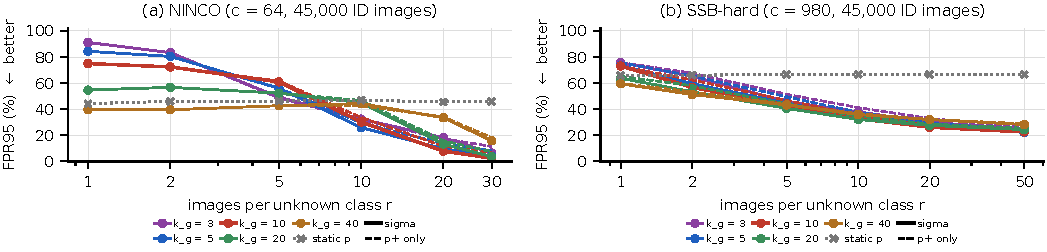
\includegraphics[width=\textwidth]{figs/fig18_kg.pdf}
\caption{近傍数$k_g$を変えた再出現の格子（\FPR{}，単体，DINOv2 L/14 + DINOv3 L/16）．実線は$\sigma$，破線は$\pP$だけ，灰色の点線は静的$p$（$k_g$に依らない）．}
\label{fig:kg}
\end{figure*}

\section{種の上限$\tau$の格子}
\label{sec:app_cap}
\tabref{caprec}に，\secref{cap}の上限付きの規則を\secref{rec}の格子の全条件で評価した\FPR{}を示す（単体，3回の平均）．混入率が低い条件ではStorey型の閾値が$\tau$に達せず，上限付きと上限なしの値は一致する．混入率30\%以上の\NCaprecNHi{}条件（SSB-hard 980クラス$\times$20，50枚）では上限付きのStorey型は$\pP$だけより\NCaprecStoreycHiMaxMinusLpAbs{}--\NCaprecStoreycHiMinMinusLpAbs{}ポイント良く，980クラス$\times$50枚では種に混じるIDの割合が\NCaprecSsbHardCNineEightZeroRFiveZeroStoreyIdfrac{}から\NCaprecSsbHardCNineEightZeroRFiveZeroStoreycIdfrac{}に下がる．全\NCaprecNCells{}条件で上限付きのStorey型が$\pP$だけより1ポイント以上悪いのは\NCaprecStoreycAllNWorseLpOne{}条件（NINCO $c{=}10,20$の$r{=}10$；上限なしも同じ値）で，そこでは種が数十枚しか選ばれず，その\NCaprecNincoCOneZeroROneZeroStoreycIdfracPct\%がIDである（未知がごく少なく$\hat\pi_0$が小さく出る条件；単純BH法は種を選ばない）．単純BH法は上限の有無に依らず全条件で$\pP$だけより最大\NCaprecBhcAllMaxMinusLp{}ポイントしか悪くならない．登録時の仮説H3（付録\ref{sec:app_hyp}：混入率30\%以上で$\pP$だけより1ポイント以上悪くならず，$r\ge10$・混入率30\%未満で上限なしの利得を1ポイント以内に保つ）は，後者の\NCaprecLoROneZeroN{}条件での差が最大\NCaprecLoROneZeroMaxStoreycMinusStorey{}ポイントであり，成り立つ．


\begin{table*}[t]
\centering
\caption{種の上限$\tau{=}0.05$の規則の格子（\FPR{}[\%]，単体，3回の平均）．Storey型・単純BH法はそれぞれ上限なし／あり．種はDINOv3 L/16のビューで上限付きStorey型に選ばれた枚数（2つの折の合計）とそのうちIDの割合（\%）．}
\label{tab:caprec}
\vspace{1.5mm}
{\fontsize{6.3pt}{7.4pt}\selectfont\renewcommand{\arraystretch}{1.0}%
\setlength{\tabcolsep}{2.2pt}\begin{tabular}{@{}rrr|cc|cc|c|c|cc@{}}
\hline
\rule[-2.0pt]{0pt}{8.2pt} & & & \multicolumn{2}{c|}{Storey型} & \multicolumn{2}{c|}{単純BH法} & & & \multicolumn{2}{c}{種（上限付きStorey型）} \\
\rule[-2.0pt]{0pt}{8.2pt}$c$ & $r$ & 混入率 & 上限なし & $\tau{=}0.05$ & 上限なし & $\tau{=}0.05$ & $\pP$のみ & 静的$p$ & 枚数 & ID \\
\hline
\multicolumn{10}{@{}l}{\rule{0pt}{6.6pt}\textit{NINCO}} \\
5 & 1 & 0.0 & 73.3 & 73.3 & 73.3 & 73.3 & 73.3 & 33.3 & 0 & -- \\
5 & 2 & 0.0 & 76.7 & 76.7 & 76.7 & 76.7 & 76.7 & 63.3 & 0 & -- \\
5 & 5 & 0.1 & 76.0 & 76.0 & 76.0 & 76.0 & 76.0 & 46.7 & 0 & -- \\
5 & 10 & 0.1 & 40.7 & 40.7 & 40.7 & 40.7 & 40.7 & 69.3 & 35 & 81.9 \\
5 & 20 & 0.2 & 11.7 & 11.7 & 9.7 & 9.7 & 10.7 & 43.3 & 91 & 71.2 \\
5 & 30 & 0.3 & 10.9 & 10.9 & 12.0 & 12.0 & 14.4 & 34.2 & 189 & 58.8 \\
10 & 1 & 0.0 & 73.3 & 73.3 & 73.3 & 73.3 & 73.3 & 33.3 & 0 & -- \\
10 & 2 & 0.0 & 78.3 & 78.3 & 78.3 & 78.3 & 78.3 & 55.0 & 0 & -- \\
10 & 5 & 0.1 & 70.7 & 70.7 & 70.7 & 70.7 & 70.7 & 52.7 & 0 & -- \\
10 & 10 & 0.2 & 28.7 & 28.7 & 26.7 & 26.7 & 26.7 & 45.7 & 70 & 79.1 \\
10 & 20 & 0.4 & 8.8 & 8.8 & 10.0 & 10.0 & 10.7 & 39.2 & 232 & 53.8 \\
10 & 30 & 0.7 & 1.4 & 1.4 & 2.0 & 2.0 & 4.9 & 35.1 & 436 & 50.3 \\
20 & 1 & 0.0 & 60.0 & 60.0 & 60.0 & 60.0 & 60.0 & 35.0 & 0 & -- \\
20 & 2 & 0.1 & 77.5 & 77.5 & 77.5 & 77.5 & 77.5 & 40.0 & 0 & -- \\
20 & 5 & 0.2 & 68.0 & 68.0 & 68.0 & 68.0 & 68.0 & 45.7 & 0 & -- \\
20 & 10 & 0.4 & 36.2 & 36.2 & 34.7 & 34.7 & 34.7 & 44.5 & 35 & 71.7 \\
20 & 20 & 0.9 & 9.0 & 9.0 & 8.5 & 8.5 & 11.8 & 52.5 & 415 & 46.1 \\
20 & 30 & 1.3 & 3.9 & 3.9 & 4.3 & 4.3 & 6.9 & 45.6 & 955 & 48.8 \\
40 & 1 & 0.1 & 75.8 & 75.8 & 75.8 & 75.8 & 75.8 & 47.5 & 0 & -- \\
40 & 2 & 0.2 & 70.8 & 70.8 & 70.8 & 70.8 & 70.8 & 46.2 & 0 & -- \\
40 & 5 & 0.4 & 67.8 & 67.8 & 67.8 & 67.8 & 67.8 & 46.5 & 0 & -- \\
40 & 10 & 0.9 & 35.2 & 35.2 & 34.5 & 34.5 & 34.5 & 48.9 & 175 & 58.5 \\
40 & 20 & 1.7 & 9.8 & 9.8 & 10.2 & 10.2 & 12.9 & 49.8 & 1081 & 47.5 \\
40 & 30 & 2.6 & 2.7 & 2.7 & 3.2 & 3.2 & 5.9 & 45.1 & 1766 & 41.5 \\
64 & 1 & 0.1 & 75.0 & 75.0 & 75.0 & 75.0 & 75.0 & 44.3 & 0 & -- \\
64 & 2 & 0.3 & 72.4 & 72.4 & 72.4 & 72.4 & 72.4 & 46.1 & 0 & -- \\
64 & 5 & 0.7 & 60.9 & 60.9 & 61.6 & 61.6 & 61.6 & 46.2 & 33 & 74.5 \\
64 & 10 & 1.4 & 30.2 & 30.2 & 30.5 & 30.5 & 33.7 & 46.9 & 296 & 46.2 \\
64 & 20 & 2.8 & 7.9 & 7.9 & 7.7 & 7.7 & 11.7 & 45.5 & 1689 & 41.5 \\
64 & 30 & 4.1 & 2.5 & 2.5 & 2.9 & 2.9 & 6.7 & 46.0 & 2664 & 36.6 \\
\multicolumn{10}{@{}l}{\rule{0pt}{6.6pt}\textit{SSB-hard}} \\
10 & 1 & 0.0 & 90.0 & 90.0 & 90.0 & 90.0 & 90.0 & 66.7 & 0 & -- \\
10 & 2 & 0.0 & 86.7 & 86.7 & 86.7 & 86.7 & 86.7 & 73.3 & 0 & -- \\
10 & 5 & 0.1 & 82.0 & 82.0 & 82.0 & 82.0 & 82.0 & 53.3 & 0 & -- \\
10 & 10 & 0.2 & 60.0 & 60.0 & 60.0 & 60.0 & 60.0 & 63.3 & 0 & -- \\
10 & 20 & 0.4 & 45.8 & 45.8 & 47.0 & 47.0 & 46.8 & 69.8 & 122 & 64.8 \\
10 & 50 & 1.1 & 11.5 & 11.5 & 11.1 & 11.1 & 18.1 & 65.7 & 535 & 48.5 \\
30 & 1 & 0.1 & 71.1 & 71.1 & 71.1 & 71.1 & 71.1 & 55.6 & 0 & -- \\
30 & 2 & 0.1 & 82.8 & 82.8 & 82.8 & 82.8 & 82.8 & 65.0 & 0 & -- \\
30 & 5 & 0.3 & 79.1 & 79.1 & 79.1 & 79.1 & 79.1 & 65.1 & 0 & -- \\
30 & 10 & 0.7 & 60.7 & 60.7 & 60.3 & 60.3 & 60.3 & 58.9 & 72 & 77.0 \\
30 & 20 & 1.3 & 43.3 & 43.3 & 43.5 & 43.5 & 46.4 & 71.0 & 344 & 51.4 \\
30 & 50 & 3.2 & 16.5 & 16.5 & 16.3 & 16.3 & 25.1 & 67.3 & 1507 & 41.9 \\
100 & 1 & 0.2 & 80.0 & 80.0 & 80.0 & 80.0 & 80.0 & 65.0 & 0 & -- \\
100 & 2 & 0.4 & 84.0 & 84.0 & 84.0 & 84.0 & 84.0 & 71.0 & 0 & -- \\
100 & 5 & 1.1 & 76.1 & 76.1 & 75.8 & 75.8 & 75.8 & 70.3 & 33 & 87.9 \\
100 & 10 & 2.2 & 50.7 & 50.7 & 51.5 & 51.5 & 56.5 & 68.1 & 404 & 55.2 \\
100 & 20 & 4.3 & 32.4 & 32.4 & 33.3 & 33.3 & 38.5 & 66.9 & 1597 & 44.2 \\
100 & 50 & 10 & 18.5 & 18.5 & 18.7 & 18.7 & 24.2 & 67.2 & 5132 & 31.6 \\
300 & 1 & 0.7 & 78.6 & 78.6 & 78.6 & 78.6 & 78.6 & 67.1 & 0 & -- \\
300 & 2 & 1.3 & 73.6 & 73.6 & 73.6 & 73.6 & 73.6 & 64.7 & 0 & -- \\
300 & 5 & 3.2 & 58.9 & 58.9 & 58.7 & 58.7 & 62.2 & 64.6 & 402 & 49.7 \\
300 & 10 & 6.2 & 42.3 & 42.3 & 42.8 & 42.8 & 47.9 & 66.8 & 1751 & 38.0 \\
300 & 20 & 12 & 29.7 & 29.7 & 29.9 & 29.9 & 34.2 & 65.7 & 5348 & 32.2 \\
300 & 50 & 25 & 19.3 & 19.6 & 19.6 & 19.6 & 22.1 & 66.9 & 14736 & 19.1 \\
980 & 1 & 2.1 & 73.1 & 73.1 & 72.9 & 72.9 & 72.9 & 65.9 & 33 & 84.7 \\
980 & 2 & 4.2 & 56.8 & 56.8 & 56.5 & 56.5 & 62.4 & 66.1 & 522 & 47.5 \\
980 & 5 & 9.8 & 43.1 & 43.1 & 42.7 & 42.7 & 46.7 & 66.6 & 3381 & 36.1 \\
980 & 10 & 18 & 32.8 & 32.8 & 32.6 & 32.6 & 35.5 & 66.7 & 9372 & 31.0 \\
980 & 20 & 30 & 26.2 & 26.1 & 26.1 & 26.1 & 27.8 & 66.8 & 17485 & 16.7 \\
980 & 50 & 52 & 22.6 & 22.2 & 21.5 & 22.2 & 23.4 & 66.6 & 40958 & 6.6 \\
\hline
\end{tabular}}%

\end{table*}

\section{追加実験の事前登録と仮説の判定}
\label{sec:app_hyp}
\secref{cap}の上限付きの種，\secref{in200}の全学習画像・ゼロショットの基線，付録\ref{sec:app_kg}の$k_g$の格子，付録\ref{sec:app_views}の中心化は，1つの登録文書（公開リポジトリの\texttt{experiments/phase15/prereg\_p15.json}，SHA-256 \texttt{83ea4061}$\cdots$）に計算の内容・報告の形・6つの仮説を記してから実行した．登録文書は評価の実行前に公開リポジトリのブランチ\texttt{phase12-15-registrations}（コミット\texttt{8ef9c8d}）にコミットし，その時刻が第三者の確認できる時刻である（学習画像の特徴抽出だけはコミット前に始めた）．構成の選択は行わず（$\tau$と$q$は固定，本稿の主構成は変えない），登録からの逸脱はない．系1の実測（付録\ref{sec:app_kg}）は査読後に加えた登録外の記述的な計算で，選択を含まない．判定は次のとおりである．
\textbf{H1}（上限は害を消す：CIFAR-100 far-OODとImageNet-200 near-OODで上限付きの規則は$\pP$だけの+0.5ポイント以内）：成立（+\NCifarStoreycFarDfprVsLp{}，\NInTwoZeroZeroStoreycNearDfprVsLp{}ポイント）．
\textbf{H2}（上限はImageNet-1K near-OODで上限なしの0.5ポイント以内）：成立（単体\NCapStoreycAloneNearDfprVsStorey{}，$\times$TINS +\NCapStoreycNearDfprVsStorey{}ポイント）．
\textbf{H3}（格子：混入率30\%以上で$\pP$だけより1ポイント以上悪くならず，$r\ge10$・混入率30\%未満で上限なしの利得を1ポイント以内に保つ）：成立（付録\ref{sec:app_cap}）．
\textbf{H4}（全学習画像のkNN（$k{=}50$）は両ベンチマークで16枚の静的$p$より良く，ImageNet-200のnear-OODでは$\sigma$がkNNより低い\FPR{}を保つ）：前半は否定（ImageNet-200でkNN \NInTwoZeroZeroKnnAllKFiveZeroNearFpr\%／\NInTwoZeroZeroKnnAllKFiveZeroFarFpr\%対静的$p$ \NInTwoZeroZeroStaticNearFpr\%／\NInTwoZeroZeroStaticFarFpr\%，CIFAR-100のfar-OODで\NCifarKnnAllKFiveZeroFarFpr\%対\NCifarStaticFarFpr\%；CIFAR-100のnear-OODだけ\NCifarKnnAllKFiveZeroNearFpr\%対\NCifarStaticNearFpr\%），後半は成立（\NInTwoZeroZeroMainNearFpr\%対\NInTwoZeroZeroKnnAllKFiveZeroNearFpr\%）．
\textbf{H5}（$\sigma$が静的$p$を下回る$r$は$k_g$が小さいほど小さく，大きい$r$での利得は$k_g\in\{10,20\}$で最大）：前半は否定，後半は$\{5,10\}$として部分的に成立（付録\ref{sec:app_kg}）．
\textbf{H6}（中心化でCLIPの静的$p$はDINO系の範囲（near 70\%未満，far 40\%未満）に入り，DINO系の変化は10ポイント以内）：前半は否定（near \NViewClipStaticcNearFpr\%，far \NViewClipStaticcFarFpr\%），後半は静的$p$で成立（最大\NViewsDinoCentredMaxabsFpr{}ポイント），kNNではDINO (v1)のfar-OODで\NViewsDinoKnncentredMaxabsFpr{}ポイント動く．

\end{document}
